\documentclass[10pt,twoside,openright]{report}

\usepackage{amsmath}
\usepackage[utf8]{inputenc}
\usepackage{graphicx}
\usepackage{tikz} 
\usepackage{bbold}
\usetikzlibrary{shapes,arrows,positioning,automata,backgrounds,calc,er,patterns}
\usepackage{breqn}
\usepackage{enumitem}
\usepackage{dsfont}
\usepackage{subfig}
\usepackage{lscape}
\usepackage{multirow}
\usepackage{color, colortbl}
\usepackage[a4paper,width=130mm,top=50mm,bottom=40mm]{geometry}
\usepackage{setspace}
\usepackage{epigraph}
\renewcommand{\textflush}{flushright}
\usepackage[super]{nth}
\onehalfspacing
\usepackage{fancyhdr}
\pagestyle{fancy}
\fancyhead[lo]{\nouppercase{\rightmark}}
\fancyhead[re]{\nouppercase{\leftmark}}
\fancyhead[ro,le]{\thepage}
\cfoot{}
\renewcommand{\headrulewidth}{1pt}
\usepackage{url}
\usepackage[backend=biber,style=numeric-comp,sorting=none]{biblatex}
\usepackage[hidelinks]{hyperref}
\usepackage{xspace}

%Figure and table caption style
\usepackage[font=small, labelfont=bf, justification=raggedright, format=hang]{caption}

%colours for yields table
\definecolor{Gray}{gray}{0.90}

\definecolor{VBF0}{rgb}{1,0.7,0.7}
\definecolor{VBF1}{rgb}{1,0.8,0.8}
\definecolor{VBF2}{rgb}{1,0.9,0.9}

\definecolor{GGH0}{rgb}{0.6,0.6,1.0}
\definecolor{GGH1}{rgb}{0.7,0.7,1.0}
\definecolor{GGH2}{rgb}{0.8,0.8,1.0}
\definecolor{GGH3}{rgb}{0.9,0.9,1.0}

\definecolor{VHH}{rgb}{0.8,1.0,0.8}
\definecolor{VHM}{rgb}{0.9,1.0,0.9}

%bibliography
\addbibresource{bibliography}

%useful commands
\newcommand{\pt}{\ensuremath{p_T}\xspace}
\newcommand{\SUN}{\ensuremath{\mathrm{SU}(N)}\xspace}
\newcommand{\MET}{\ensuremath{E_{T}^{\mathrm{miss}}}\xspace}
\newcommand{\Hgg}{\ensuremath{\mathrm{H}\,\rightarrow\,\gamma\gamma}\xspace}
\newcommand{\Zee}{\ensuremath{\mathrm{Z}\rightarrow{\mathrm{e}^{+}\mathrm{e}^{-}}}\xspace}
\newcommand{\Zmumu}{\ensuremath{\mathrm{Z}\rightarrow{\mu^{+}\mu^{-}}}\xspace}
\newcommand{\ttH}{\ensuremath{\mathrm{t}\bar{\mathrm{t}}\mathrm{H}}\xspace}
\newcommand{\mgg}{\ensuremath{m_{\gamma\gamma}}\xspace}
\newcommand{\mH}{\ensuremath{m_{H}}\xspace}
\newcommand{\Etrue}{\ensuremath{E_{\mathrm{true}}}\xspace}
\newcommand{\Eraw}{\ensuremath{E_{SC}}\xspace}
\newcommand{\fb}{\ensuremath{\textrm{fb}^{-1}}\xspace}
\newcommand{\pbw}{\ensuremath{\textrm{PbWO}_4}\xspace}
\newcommand{\met}{\ensuremath{E^\textrm{miss}_{T}}\xspace}

%thicker hline in tables
\makeatletter
\def\thickhline{%
  \noalign{\ifnum0=`}\fi\hrule \@height \thickarrayrulewidth \futurelet
   \reserved@a\@xthickhline}
\def\@xthickhline{\ifx\reserved@a\thickhline
               \vskip\doublerulesep
               \vskip-\thickarrayrulewidth
             \fi
      \ifnum0=`{\fi}}
\makeatother

%I've forgotten what this does
%possibly removes headers on blank pages
\makeatletter
\renewcommand*{\cleardoublepage}{\clearpage\if@twoside \ifodd\c@page\else
\hbox{}%
\thispagestyle{plain}%
\newpage%
\if@twocolumn\hbox{}\newpage\fi\fi\fi}
\makeatother

%Bold maths in subsection titles
\makeatletter
\g@addto@macro\bfseries{\boldmath}
\makeatother

\newlength{\thickarrayrulewidth}
\setlength{\thickarrayrulewidth}{2\arrayrulewidth}


\begin{document}

\begin{titlepage}
    \begin{center}
        \vspace*{2cm}
        
        \huge{\textbf{Precision measurements of Higgs boson properties with beyond the standard model interpretations at the CMS experiment}}

        \vspace{1.5cm}
        \normalsize
        Jonathon Mark Langford
        
        \vspace{0.5cm}
        Imperial College London\\
        Department of Physics\\

        \vspace{5cm}
        A thesis submitted to Imperial College London\\
        for the degree of Doctor of Philosophy\\
        
    \end{center}
\end{titlepage}

The copyright of this thesis rests with the author and is made available under a Creative Commons Attribution Non-Commercial No Derivatives licence. Researchers are free to copy, distribute or transmit the thesis on the condition that they attribute it, that they do not use it for commercial purposes and that they do not alter, transform or build upon it. For any reuse or redistribution, researchers must make clear to others the licence terms of this work.


\pagenumbering{roman}
\chapter*{\centering Abstract}
Measurements of Higgs boson production cross sections 
with the Higgs boson decaying into a pair of photons are reported.
Events with two photons are selected from a sample of proton-proton collisions 
at a centre-of-mass energy of \SI{13}{TeV} 
collected by the Compact Muon Solenoid detector at the Large Hadron Collider in 2016 and 2017,
corresponding to a total integrated luminosity of $77.4~\mathrm{fb}^{-1}$.
Cross sections for gluon fusion and vector boson fusion production, 
normalised to the corresponding standard model predictions,
are measured to be $1.15 \pm 0.15$ and $0.83_{-0.31}^{+0.37}$ respectively.
These two production modes are further measured in kinematic regions 
within the simplified template cross section framework.
All results are found to be in agreement with the standard model expectations~\cite{HIG-18-029}.


\chapter*{\centering }% Dedication}
\begin{center}
    \thispagestyle{empty}
    To Mum and Dad
\end{center}


\chapter*{\centering Declaration}
The work contained within this thesis is my own. 
It was produced using existing work from, and in collaboration with, 
several individuals and the Compact Muon Solenoid (CMS) Collaboration. 
The details of the contributions relevant to each chapter are set out below;
in all cases, the work of others has been referenced appropriately.

Chapter~\ref{chap:intro} introduces our current understanding of particle physics 
and the Higgs boson in my own words.

Chapter~\ref{chap:theory} explains the theory of the Standard Model and the Higgs mechanism, 
which is the work of others, in my own words. 
The status of the latest Higgs boson measurements is summarised, 
which includes my own work on the CMS \Hgg analysis based on the 2016 dataset~\cite{HIG-16-040}.

Chapter~\ref{chap:detector} describes the CMS detector, 
which was designed, built, and operated by others, in my own words.

Chapter~\ref{chap:hgcal} describes the High Granularity Calorimeter (HGCAL), 
the design and testing of which is the work of others within the CMS collaboration. 
The section on reconstruction is based on my own work, 
which was performed together with Lindsey Gray, Clemens Lange and Emilio Meschi~\cite{ClusteringConf}.
The demonstration of the HGCAL's potential for a vector boson fusion analysis 
in the \Hgg decay channel is my own work~\cite{HGCAL}.

Chapters~\ref{chap:objects}-\ref{chap:results} describe the methodology and results of the CMS \Hgg analysis
which constitute the main part of this thesis and consist primarily of my own work.
This analysis has also been documented in Ref.~\cite{HIG-18-029}.
The detailed breakdown of each chapter is given below.

Chapter~\ref{chap:objects} describes how events are reconstructed at CMS.
These techniques were developed and optimised by others within the \Hgg analysis group 
and the CMS collaboration, but are summarised in my own words.

Chapter~\ref{chap:categorisation} describes the categorisation of events 
to maximise the sensitivity of the analysis.
This is my own work, and is based on the strategies adopted in previous CMS \Hgg analyses.
The data-driven method for the training of the dijet boosted decision tree 
was initially developed by Yacine Haddad, and was implemented in this analysis by Shameena Bonomally.

Chapter~\ref{chap:sigbkg} describes the construction of the signal and background models, 
and the various uncertainties included in the analysis.
This is my own work, although the techniques utilised were first developed by others.

Chapter~\ref{chap:results} reports the final observed results and their uncertainties.
This is also my own work, but the methods and tools used are originally the work of others.

Chapter~\ref{chap:conclusions} summarises the work done in this thesis 
and the implications of the results.
This is done in my own words and with my own considerations for the future development of this work.

\begin{flushright}
    Edward John Titman Scott
\end{flushright}


\chapter*{\centering Acknowledgements}
Acknowledgements go here.
%STFC & CERN
%CMS Hgg group, especially the conveners?
%IC Hgg group; names?
%Seth
%Gavin
%Chris
%Nick
%Friends at IC and at CERN: keeping sanity, getting a beer, and decent magret de canard
%Friends at home: loyalty, support, laughter, etc
%M and D; thank you for everything. 
%This was more often in the form of driving to Croydon for basketball practices
%than encouraging me to wonder about physics, but it had the same effect.
%You always encouraged me to pursue anything that I wanted to pursue, 
%and made me believe it was worth doing so.
%Ari


\tableofcontents
\listoffigures
\listoftables


%\chapter*{}
%\epigraph{
%  \textit{``And once you have tasted flight, \\ \\
%            you will walk the Earth \\ \\
%            with your eyes turned skyward; \\ \\
%            for there you have been, \\ \\
%            and there you long to return''}}
%         {Leonardo da Vinci}


\cleardoublepage


\pagenumbering{arabic}
\chapter{Introduction}
\label{chap:intro}

The Standard Model (SM) of particle physics is a theory which describes
the fundamental structure of matter and its interactions.
Guided by the results of experiments studying the behaviour of high-energy particles, 
the SM places unifies the electromagnetic and weak forces and places them in a coherent framework
together with the strong force.
The SM has been extraordinarily successful, 
with many of its predictions verified to unprecedented precision.
A key aspect of the SM is the Higgs mechanism, 
which breaks the symmetry of the electroweak interaction, explains how particles obtain mass, 
and predicts the existence of a fundamental particle known as the Higgs boson.
The Higgs boson was observed experimentally by the ATLAS and CMS collaborations in 2012
with data collected during Run 1 of the Large Hadron Collider (LHC)~\cite{ATLASdiscovery,CMSdiscovery}.
This discovery completed the particle content and modern understanding of the SM, 
and represents another great success of the theory.

The SM is however known to be incomplete as a theory of nature.
Firstly, it does not include a description of the force of gravity.
The SM also does not provide a suitable candidate for dark matter, 
which is required to explain certain astrophysical phenomena~\cite{BulletCluster},
and forms a key part of the modern understanding 
of the large scale structure of the universe~\cite{Planck}.
Furthermore, in the SM neutrinos are treated as massless, 
whereas experimental measurements of neutrino oscillations confirm that they are not~\cite{NeutrinoOscillation}.
A wide range of extensions to the SM have been proposed 
which provide explanations for some or all of these phenomena~\cite{SUSY}.
These beyond standard model (BSM) theories can predict the existence of entirely new particles, 
and thereby modify the predictions made by the SM.

The results presented in this thesis test the SM predictions of Higgs boson production
in the diphoton decay channel with the CMS experiment.
Data collected as part of Run~2 of the LHC during 2016 and 2017 is analysed, 
yielding a dataset of \SI{77.4}{\fbinv}.
The CMS detector is a multi-purpose apparatus able to reconstruct several types of high-energy particles.
Its design is motivated in part by the objective of precisely measuring properties of the Higgs boson.
In particular, the performance of its electromagnetic calorimeter is excellent, 
which enables effective reconstruction of the photons arising from the decay of the Higgs 
and is vital for the success of the \Hgg analysis.
The final results of the analysis are measurements of Higgs boson production cross sections
within the simplified template cross section (STXS) framework.
The STXS framework provides a coherent approach to performing measurements of Higgs boson properties, 
minimising the effect of theoretical uncertainties 
whilst simultaneously permitting the use of advanced experimental techniques.
Results within the STXS framework are presented
which aim to test the SM prediction as stringently as possible.
Deviations from the SM predictions may indicate the presence of BSM physics 
and guide the way to an improved understanding of nature, 
or otherwise tightly constrain the possible forms BSM theories can take.

This thesis presents results of the CMS \Hgg analysis using 2016 and 2017 data, 
which is documented in Ref.~\cite{HIG-18-029}.
The structure of the thesis is as follows.

Chapter~\ref{chap:theory} describes the structure of the SM as a gauge field theory, 
before introducing the Higgs mechanism and its implications.
The phenomenology of the Higgs boson and its decay into two photons is discussed, 
and the latest measurements of Higgs boson properties, including those within the STXS framework, 
are summarised.

Chapter~\ref{chap:detector} describes the structure of the LHC and of the CMS detector itself.
The role of each subdetector and how they capture the various products 
of high energy proton-proton collisions is explained.

Chapter~\ref{chap:hgcal} describes the planned upgrade program for the LHC to become the High-Luminosity LHC (HL-LHC) 
and the required changes to the CMS detector, focusing on the High Granularity Calorimeter (HGCAL).
The motivation for and design of the HGCAL is presented, 
together with studies illustrating its performance in object reconstruction and physics analysis.

Chapter~\ref{chap:objects} describes how events recorded by the CMS detector are reconstructed.
Emphasis is placed on the procedures used to form photon objects, 
and how they are subsequently combined with a vertex hypothesis to form diphoton candidates 
for \Hgg analysis.

Chapter~\ref{chap:categorisation} describes the procedure for categorising events in the \Hgg analysis.
Analysis categories targeting different production processes are defined, 
and the sensitivity of the analysis improved 
using machine learning techniques to discriminate between signal and background processes.

Chapter~\ref{chap:sigbkg} describes the construction of models for the signal and background 
contributions to the diphoton invariant mass distributions of the final analysis categories.
The treatment of systematic uncertainties in the analysis is also detailed.

Chapter~\ref{chap:results} describes the statistical fitting procedure used 
to extract the final results of the analysis and their associated uncertainties.
Results of cross sections at different levels of granularity within the STXS framework 
are presented, and comparisons made to the corresponding SM predictions.

Finally, Chapter~\ref{chap:conclusions} discusses the conclusions drawn from the results of the analysis, 
and provides a perspective on future work to build on those results.

\chapter{Theory}
\label{chap:theory}

\section{The standard model of particle physics}
\begin{itemize}
    \item Lagrangian formalism. Smooth transition to EFT.
\end{itemize}

\section{Higgs boson phenomenology}
Different production mechanisms. ttH, tH as means for measuring the top yukawa directly, ggH is indirect. Higgs self coupling. Throughout, no distinction between quark and antiquark.

\section{Simplified template cross sections}\label{sec:theory_stxs}
qqH definition. ggZH had grouping with ggH. Define: Truth-level (consider changing to particle level) vs Reco-level. Jet definition. Drop GeV in definitions throughout. Cite STXS.

\begin{landscape}
\begin{figure}[htbp]
  \centering
  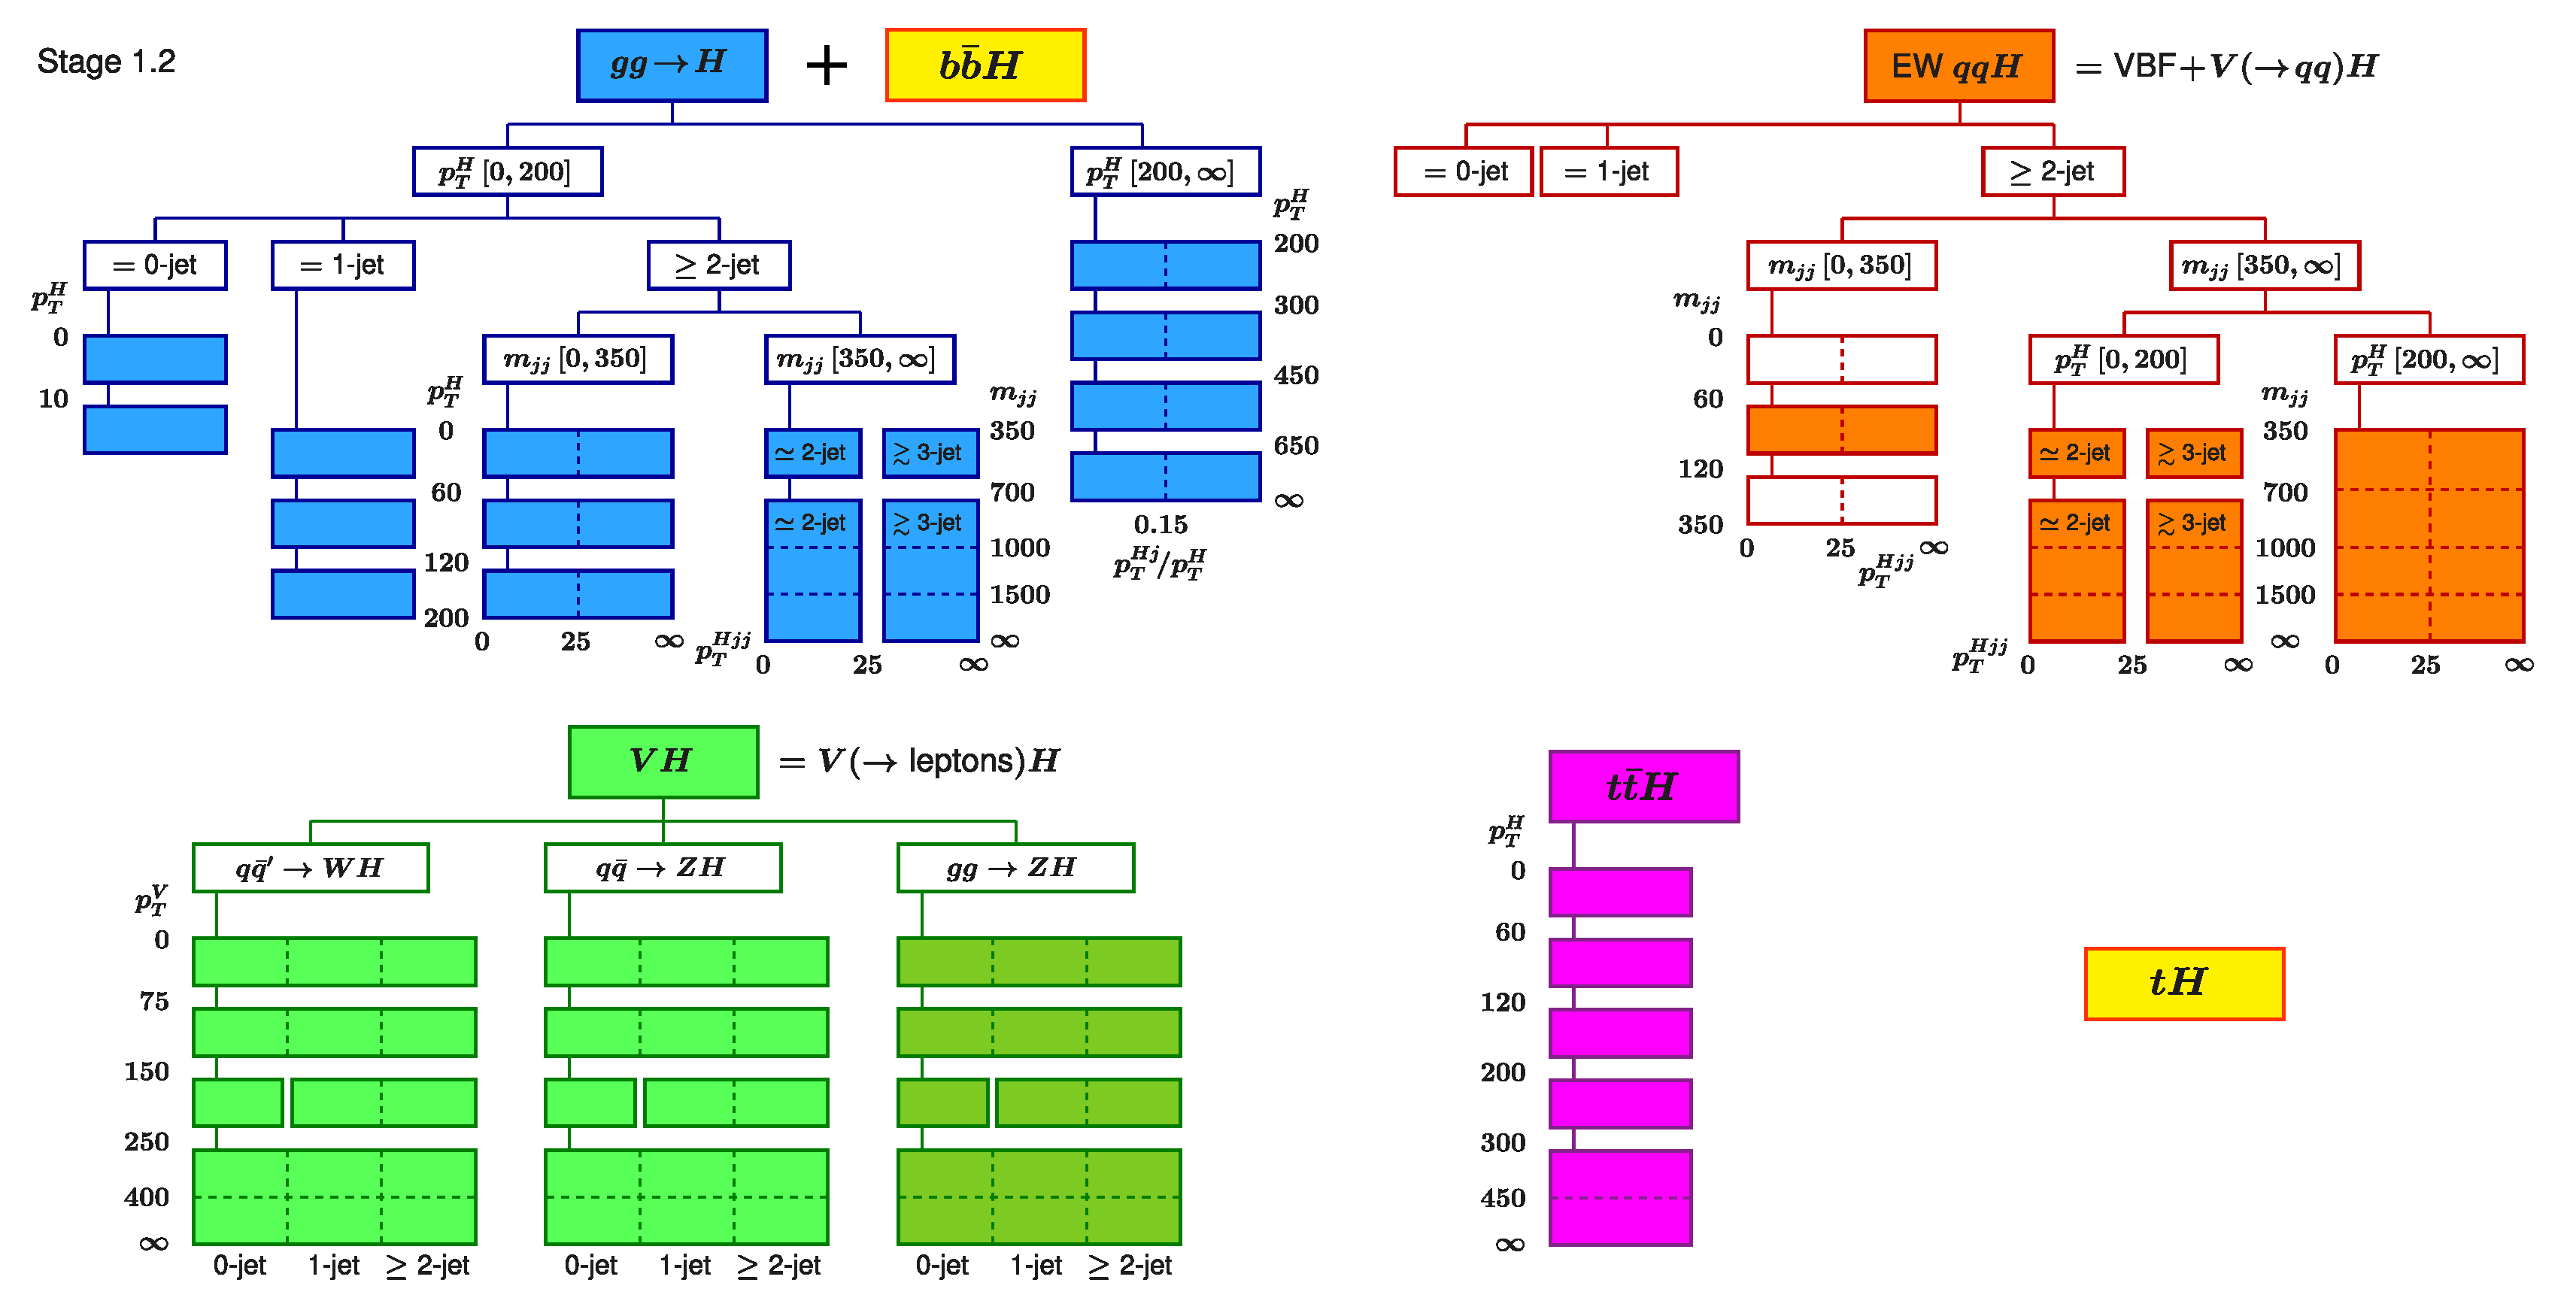
\includegraphics[width=1\linewidth]{Figures/theory/stxs_schematic.pdf}
  \caption[STXS stage 1.2 binning scheme]
  {
    A schematic showing the complete STXS stage 1.2 binning scheme. The solid lines define each stage 1.2 bin. The ggH region (blue) is split into bins using the Higgs boson transverse momentum, \ptH, the number of jets, and an additional VBF-like region with high dijet invariant mass, \mjj. The VBF and VH hadronic production modes are considered together as EW qqH production (orange). The bins here are deined using \ptH, the number of jets, \mjj, and the transverse momentum of the Higgs boson plus dijet system, \ptHjj, in the VBF-like region. The VH leptonic bins (green) are defined by the number of jets and the transverse momentum of the vector boson, \ptV. The ttH production mode (magenta) is split only by \ptH. Finally, the tH and bbH processes (yellow) are not further divided at STXS stage 1.2. In this analysis, bbH is grouped with the definition of ggH.
  }
  \label{fig:stxs_schematic}
\end{figure}
\end{landscape}


\begin{table}[htb!]
    \caption[ggH STXS stage 1.2 definitions and fractions]{Make clear definitions of jets etc  distance param}
    \label{tab:ggH_definitions}
    % \vspace{.5cm}
    \centering
    \scriptsize
    \renewcommand{\arraystretch}{1.2}
    \setlength{\tabcolsep}{5pt}
    \hspace*{-5cm}
    \begin{tabular}{l|cccc}
   \multirow{2}{*}{STXS bin} & \multirow{2}{*}{\begin{tabular}[c]{@{}c@{}}Definition\\ units of $\ptH$, $\mjj$ and $\ptHjj$ in GeV\end{tabular}} & \multicolumn{2}{c}{Fraction of cross section} & \multirow{2}{*}{$\sigma_{\text{SM}}\mathcal{B}$~(fb)} \\
    &  & ggH & gg $\rightarrow$ Z(q$\bar{\rm{q}}$)H &  \\ [\cmsTabSkip] \hline
   ggH forward & $|Y_H| > 2.5$ & 8.09\% & 2.73\% & 8.93 \\ [\cmsTabSkip]
   ggH 0J low $\ptH$ & Exactly 0 jets, $\ptH$~$<$~10 & 13.87\% & 0.01\% & 15.30 \\
   ggH 0J high $\ptH$ & Exactly 0 jets, 10~$<$~$\ptH$~$<$~200 & 39.40\% & 0.29\% & 43.45 \\ [\cmsTabSkip]
   ggH 1J low $\ptH$ & Exactly 1 jet, $\ptH$~$<$~60 & 14.77\% & 2.00\% & 16.29 \\
   ggH 1J med $\ptH$ & Exactly 1 jet, 60~$<$~$\ptH$~$<$~120 & 10.23\% & 5.34\% & 11.29 \\
   ggH 1J high $\ptH$ & Exactly 1 jet, 120~$<$~$\ptH$~$<$~200 & 1.82\% & 3.53\% & 2.01 \\  [\cmsTabSkip]
   ggH $\geq$2J low $\ptH$ & At least 2 jets, $\ptH$~$<$~60, $\mjj$~$<$~350 & 2.56\% & 5.74\% & 2.83 \\
   ggH $\geq$2J med $\ptH$ & At least 2 jets, 60~$<$~$\ptH$~$<$~120, $\mjj$~$<$~350 & 4.10\% & 19.63\% & 4.56 \\
   ggH $\geq$2J high $\ptH$ & At least 2 jets, 120~$<$~$\ptH$~$<$~200, $\mjj$~$<$~350 & 1.88\% & 29.55\% & 2.13 \\  [\cmsTabSkip]
   ggH BSM 200~$<$~$\ptH$~$<$~300 & No jet requirements, 200~$<$~$\ptH$~$<$~300 & 0.98\% & 13.93\% & 1.11 \\
   ggH BSM 300~$<$~$\ptH$~$<$~450 & No jet requirements, 300~$<$~$\ptH$~$<$~450 & 0.25\% & 3.86\% & 0.28 \\
   ggH BSM 450~$<$~$\ptH$~$<$~650 & No jet requirements, 450~$<$~$\ptH$~$<$~650 & 0.03\% & 0.77\% & 0.03 \\
   ggH BSM $\ptH$~$>$~650 & No jet requirements, $\ptH$~$>$~650 & 0.01\% & 0.20\% & 0.01 \\ [\cmsTabSkip]
   ggH VBF-like low $\mjj$ low $\ptHjj$ & \begin{tabular}[c]{@{}c@{}}At least 2 jets, $\ptH$~$<$~200,\\ 350~$<$~$\mjj$~$<$~700, $\ptHjj$~$<$~25\end{tabular} & 0.63\% & 1.14\% & 0.70 \\
   ggH VBF-like low $\mjj$ high $\ptHjj$ & \begin{tabular}[c]{@{}c@{}}At least 2 jets, $\ptH$~$<$~200,\\ 350~$<$~$\mjj$~$<$~700, $\ptHjj$~$>$~25\end{tabular} & 0.77\% & 8.06\% & 0.86 \\
   ggH VBF-like high $\mjj$ low $\ptHjj$ & \begin{tabular}[c]{@{}c@{}}At least 2 jets, $\ptH$~$<$~200,\\ $\mjj$~$>$~700, $\ptHjj$~$<$~25\end{tabular} & 0.28\% & 0.36\% & 0.31 \\
   ggH VBF-like high $\mjj$ high $\ptHjj$ & \begin{tabular}[c]{@{}c@{}}At least 2 jets, $\ptH$~$<$~200,\\ $\mjj$~$>$~700, $\ptHjj$~$>$~25\end{tabular} & 0.32\% & 2.85\% & 0.36 \\
\end{tabular}
    \hspace*{-5cm}
\end{table}

\begin{table}[htb!]
    \caption[qqH STXS stage 1.2 definitions and fractions]{Make clear definitions of jets etc distance param}
    \label{tab:qqH_definitions}
    % \vspace{.5cm}
    \centering
    \scriptsize
    \renewcommand{\arraystretch}{1.2}
    \setlength{\tabcolsep}{5pt}
    \hspace*{-5cm}
    \begin{tabular}{l|c|ccc|c}
   \multirow{2}{*}{STXS bin} & \multirow{2}{*}{\begin{tabular}[c]{@{}c@{}}Definition\\ units of $p_T^H$, $\mjj$ and $\ptHjj$ in GeV\end{tabular}} & \multicolumn{3}{c|}{Fraction of total} & \multirow{2}{*}{$\sigma_{\text{SM}}\mathcal{B}$~[fb]} \\ 
    &  & VBF & qq$\rightarrow$W(qq)H & qq$\rightarrow$Z(qq)H &  \\ [\cmsTabSkip] \hline
   qqH forward & $|Y_H| > 2.5$ & 6.69\% & 12.57\% & 9.84\% & 0.98 \\ [\cmsTabSkip]
   %\multicolumn{6}{c}{$|Y_H| < 2.5$} \\ \hline
   qqH 0J & Exactly 0 jets & 6.95\% & 5.70\% & 3.73\% & 0.77 \\ 
   qqH 1J & Exactly 1 jet & 32.83\% & 31.13\% & 25.03\% & 3.82 \\ 
   qqH $\mjj$~$<$~60 & At least 2 jets, $\mjj$~$<$~60 & 1.36\% & 3.58\% & 2.72\% & 0.23 \\ 
   qqH VH-like & At least 2 jets, 60~$<$~$\mjj$~$<$~120 & 2.40\% & 29.43\% & 28.94\% & 1.23 \\ 
   qqH 120~$<$~$\mjj$~$<$~350 & At least 2 jets, 120~$<$~$\mjj$~$<$~350 & 12.34\% & 13.92\% & 12.59\% & 1.53 \\ [\cmsTabSkip]
   qqH VBF-like low $\mjj$ low $\ptHjj$ & \begin{tabular}[c]{@{}c@{}}At least 2 jets, $\ptH$~$<$~200,\\ 350~$<$~$\mjj$~$<$~700, $\ptHjj$~$<$~25\end{tabular} & 10.26\% & 0.44\% & 0.35\% & 0.90 \\ 
   qqH VBF-like low $\mjj$ high $\ptHjj$ & \begin{tabular}[c]{@{}c@{}}At least 2 jets, $\ptH$~$<$~200,\\ 350~$<$~$\mjj$~$<$~700, $\ptHjj$~$>$~25\end{tabular} & 3.85\% & 1.86\% & 1.74\% & 0.39 \\ 
   qqH VBF-like high $\mjj$ low $\ptHjj$ & \begin{tabular}[c]{@{}c@{}}At least 2 jets, $\ptH$~$<$~200,\\ $\mjj$~$>$~700, $\ptHjj$~$<$~25\end{tabular} & 15.09\% & 0.09\% & 0.08\% & 1.30 \\ 
   qqH VBF-like high $\mjj$ high $\ptHjj$ & \begin{tabular}[c]{@{}c@{}}At least 2 jets, $\ptH$~$<$~200,\\ $\mjj$~$>$~700, $\ptHjj$~$>$~25\end{tabular} & 4.25\% & 0.40\% & 0.39\% & 0.38 \\ 
   qqH BSM & At least 2 jets, $\mjj$~$>$~350, $p_T^H$~$>$~200 & 3.98\% & 0.88\% & 0.71\% & 0.37 \\ 
\end{tabular}

    \hspace*{-5cm}
\end{table}

\begin{table}[htb!]
    \caption[VH leptonic STXS stage 1.2 definitions and fractions]{Make clear definitions of jets etc}
    \label{tab:vh_definitions}
    % \vspace{.5cm}
    \centering
    \scriptsize
    \renewcommand{\arraystretch}{1.2}
    \setlength{\tabcolsep}{5pt}
    \hspace*{-5cm}
    \begin{tabular}{l|ccccc}
    \hline
   \multirow{2}{*}{STXS bin} & \multirow{2}{*}{\begin{tabular}[c]{@{}c@{}}Definition\\ units of $\ptV$ in GeV\end{tabular}} & \multicolumn{3}{c}{Fraction of cross section} & \multirow{2}{*}{$\sigma_{\text{SM}}\mathcal{B}$~(fb)} \\
    &  & q$\bar{\rm{q}}'\rightarrow$WH & q$\bar{\rm{q}}'\rightarrow$ZH & gg$\rightarrow$ZH &  \\ [\cmsTabSkip] \hline
   WH lep forward& \multirow{3}{*}{$|Y_H| > 2.5$}& 12.13\%& -& -& 0.123 \\
   ZH lep forward& & -& 11.21\%& -& 0.058 \\
   ggZH lep forward& & -& -& 2.71\%& 0.002 \\ [\cmsTabSkip]
   %\multicolumn{6}{c}{$|Y_H| < 2.5$} \\ \hline
   WH lep $\ptV$~$<$~75 & No jet requirements, $\ptV$~$<$~75 & 46.55\% & - & - & 0.473 \\
   WH lep 75~$<$~$\ptV$~$<$~150 & No jet requirements, 75~$<$~$\ptV$~$<$~150 & 29.30\% & - & - & 0.298 \\
   WH lep 0J 150~$<$~$\ptV$~$<$~250 & Exactly 0 jets, 150~$<$~$\ptV$~$<$~250 & 5.10\% & - & - & 0.052 \\
   WH lep $\geq$1J 150~$<$~$\ptV$~$<$~250 & At least 1 jet, 150~$<$~$\ptV$~$<$~250 & 3.97\% & - & - & 0.040 \\
   WH lep $\ptV$~$>$~250 & No jet requirements, $\ptV$~$>$~250 & 2.95\% & - & - & 0.030 \\ [\cmsTabSkip]
   ZH lep $\ptV$~$<$~75 & No jet requirements, $\ptV$~$<$~75 & - & 45.65\% & - & 0.237 \\
   ZH lep 75~$<$~$\ptV$~$<$~150 & No jet requirements, 75~$<$~$\ptV$~$<$~150 & - & 30.70\% & - & 0.160 \\
   ZH lep 0J 150~$<$~$\ptV$~$<$~250 & Exactly 0 jets, 150~$<$~$\ptV$~$<$~250 & - & 5.16\% & - & 0.027 \\
   ZH lep $\geq$1J 150~$<$~$\ptV$~$<$~250 & At least 1 jet, 150~$<$~$\ptV$~$<$~250 & - & 4.27\% & - & 0.022 \\
   ZH lep $\ptV$~$>$~250 & No jet requirements, $\ptV$~$>$~250 & - & 3.01\% & - & 0.016 \\ [\cmsTabSkip]
   ggZH lep $\ptV$~$<$~75 & No jet requirements, $\ptV$~$<$~75 & - & - & 15.96\% & 0.013 \\
   ggZH lep 75~$<$~$\ptV$~$<$~150 & No jet requirements, 75~$<$~$\ptV$~$<$~150 & - & - & 43.32\% & 0.036 \\
   ggZH lep 0J 150~$<$~$\ptV$~$<$~250 & Exactly 0 jets, 150~$<$~$\ptV$~$<$~250 & - & - & 9.08\% & 0.008 \\
   ggZH lep $\geq$1J 150~$<$~$\ptV$~$<$~250 & At least 1 jet, 150~$<$~$\ptV$~$<$~250 & - & - & 20.49\% & 0.017 \\
   ggZH lep $\ptV$~$>$~250 & No jet requirements, $\ptV$~$>$~250 & - & - & 8.45\% & 0.007 \\
   \hline
\end{tabular}

    \hspace*{-5cm}
\end{table}

\begin{table}[htb!]
    \caption[Top-associated and bbH STXS stage 1.2 definitions and fractions]{Make clear definitions of jets etc}
    \label{tab:top_definitions}
    % \vspace{.5cm}
    \centering
    \scriptsize
    \renewcommand{\arraystretch}{1.5}
    \setlength{\tabcolsep}{5pt}
    \hspace*{-5cm}
    \begin{tabular}{l|c|cccc|c}
   \multirow{2}{*}{STXS region} & \multirow{2}{*}{\begin{tabular}[c]{@{}c@{}}Definition\\ units of $\ptH$ in GeV\end{tabular}} & \multicolumn{4}{c|}{Fraction of total} & \multirow{2}{*}{$\sigma_{\text{SM}}\mathcal{B}$~[fb]} \\ 
    &  & ttH & tHq & tHW & bbH &  \\ [\cmsTabSkip] \hline
   ttH forward& \multirow{3}{*}{$|Y_H| > 2.5$}& 1.35\%& -& -& -& 0.016 \\  
   tH forward& & -& 2.79\%& 1.06\%& -& 0.005 \\  
   bbH forward& & -& -& -& 4.87\%& 0.054 \\ [\cmsTabSkip] 
   %\multicolumn{7}{c}{$|Y_H| < 2.5$} \\ \hline
   ttH $\ptH$~$<$~60 & No jet requirements, $\ptH$~$<$~60 & 22.42\% & - & - & - & 0.259 \\ 
   ttH 60~$<$~$\ptH$~$<$~120 & No jet requirements, 60~$<$~$\ptH$~$<$~120 & 34.61\% & - & - & - & 0.400 \\ 
   ttH 120~$<$~$\ptH$~$<$~200 & No jet requirements, 120~$<$~$\ptH$~$<$~200 & 25.60\% & - & - & - & 0.296 \\ 
   ttH 200~$<$~$\ptH$~$<$~300 & No jet requirements, 200~$<$~$\ptH$~$<$~300 & 10.72\% & - & - & - & 0.124 \\ 
   ttH $\ptH$~$>$~300 & No jet requirements, $\ptH$~$>$~300 & 5.31\% & - & - & - & 0.061 \\ [\cmsTabSkip] 
   tH & No additional requirements & - & 97.21\% & 98.94\% & - & 0.204 \\ 
   bbH & No additional requirements & - & - & - & 95.13\% & 1.054 \\ 
\end{tabular}

    \hspace*{-5cm}
\end{table}

\section{Recent Higgs boson results}

\section{Effective field theory}\label{sec:theory_eft}

UV & IR. Replace non-local interactions via exchange of new particles by contact interactions, expressed using higher dimensional operators. This restricts validity of EFT to be below a certain energy scale. Replace below with expansion for all orders.

\begin{equation}\label{eq:eft_expansion}
    \mathcal{L}_{\rm{EFT}} = \mathcal{L}_{\rm{SM}} + \sum^{N_{\rm{dim6}}}_p \frac{c_p}{\Lambda^2}\mathcal{O}^{(6)}_p + \sum^{N_{\rm{dim8}}}_p \frac{b_p}{\Lambda^4}\mathcal{O}^{(8)}_p + ... ,
\end{equation}

\subsection{EFT basis}
\begin{itemize}
    \item Full EFT extension, only consider dim-6 in this thesis (motivations)
    \item Definition of a basis: complete and non-redundant set of operators.
    \item Lagrangian and then effect on matrix element: SM + interference + BSM. A comment on dim-8.
    \item Match EFT constraints to constrain masses and couplings in UV complete BSM theories
    \item Briefly discuss HEL and SMEFTsim: save intricate details for Chapter 7
\end{itemize}
\chapter{The Compact Muon Solenoid}
\label{chap:detector}

\section{Introduction}

The Large Hadron Collider (LHC) at CERN is a 27\,km hadron accelerator and collider with a design centre-of-mass energy of 14\,TeV~\cite{LHC}.
Its purpose is to provide collisions sufficient in energy and number to precisely probe physics at the electroweak scale.
Four detectors, one of which is the Compact Muon Solenoid (CMS), are situated around the LHC ring.
CMS is a general-purpose detector designed to precisely measure a wide range of physics objects.
Together, the LHC and CMS facilitate a wide-ranging program of physics studies, from SM precision measurements to dark matter searches, 
and including exploration of electroweak symmetry breaking via production of the Higgs boson.
This chapter will describe the design and operation of both the LHC and the CMS detector.

\section{The Large Hadron Collider}

The LHC is situated in the tunnel that previously housed the Large Electron Positron collider (LEP), 
around 100\,m below ground across the French-Swiss border near CERN.
It is the final machine in a series of accelerators which form the CERN accelerator complex; 
these  act as the injection system for the LHC.
The two counter-circulating beams cross at four interaction points, at each of which a detector is situated.
Directly opposite CMS is a second general purpose detector, ATLAS~\cite{ATLAS}, 
whose physics objectives are identical to those of CMS but with different design decisions.
The other two detectors, LHCb~\cite{LHCb} and ALICE~\cite{ALICE}, focus on flavour and heavy-ion physics respectively.
Whilst the LHC is capable of producing heavy ion collisions in addition to proton-proton collisions, 
the remainder of this section will be dedicated to its proton-proton operations.
A schematic of the full CERN accelerator complex and the LHC experiments is shown in Figure~\ref{fig:detector_CERNschematic}.
The operation of the LHC and the data it has accumulated so far is described in detail below.

\begin{figure}[h!]
  \centering
  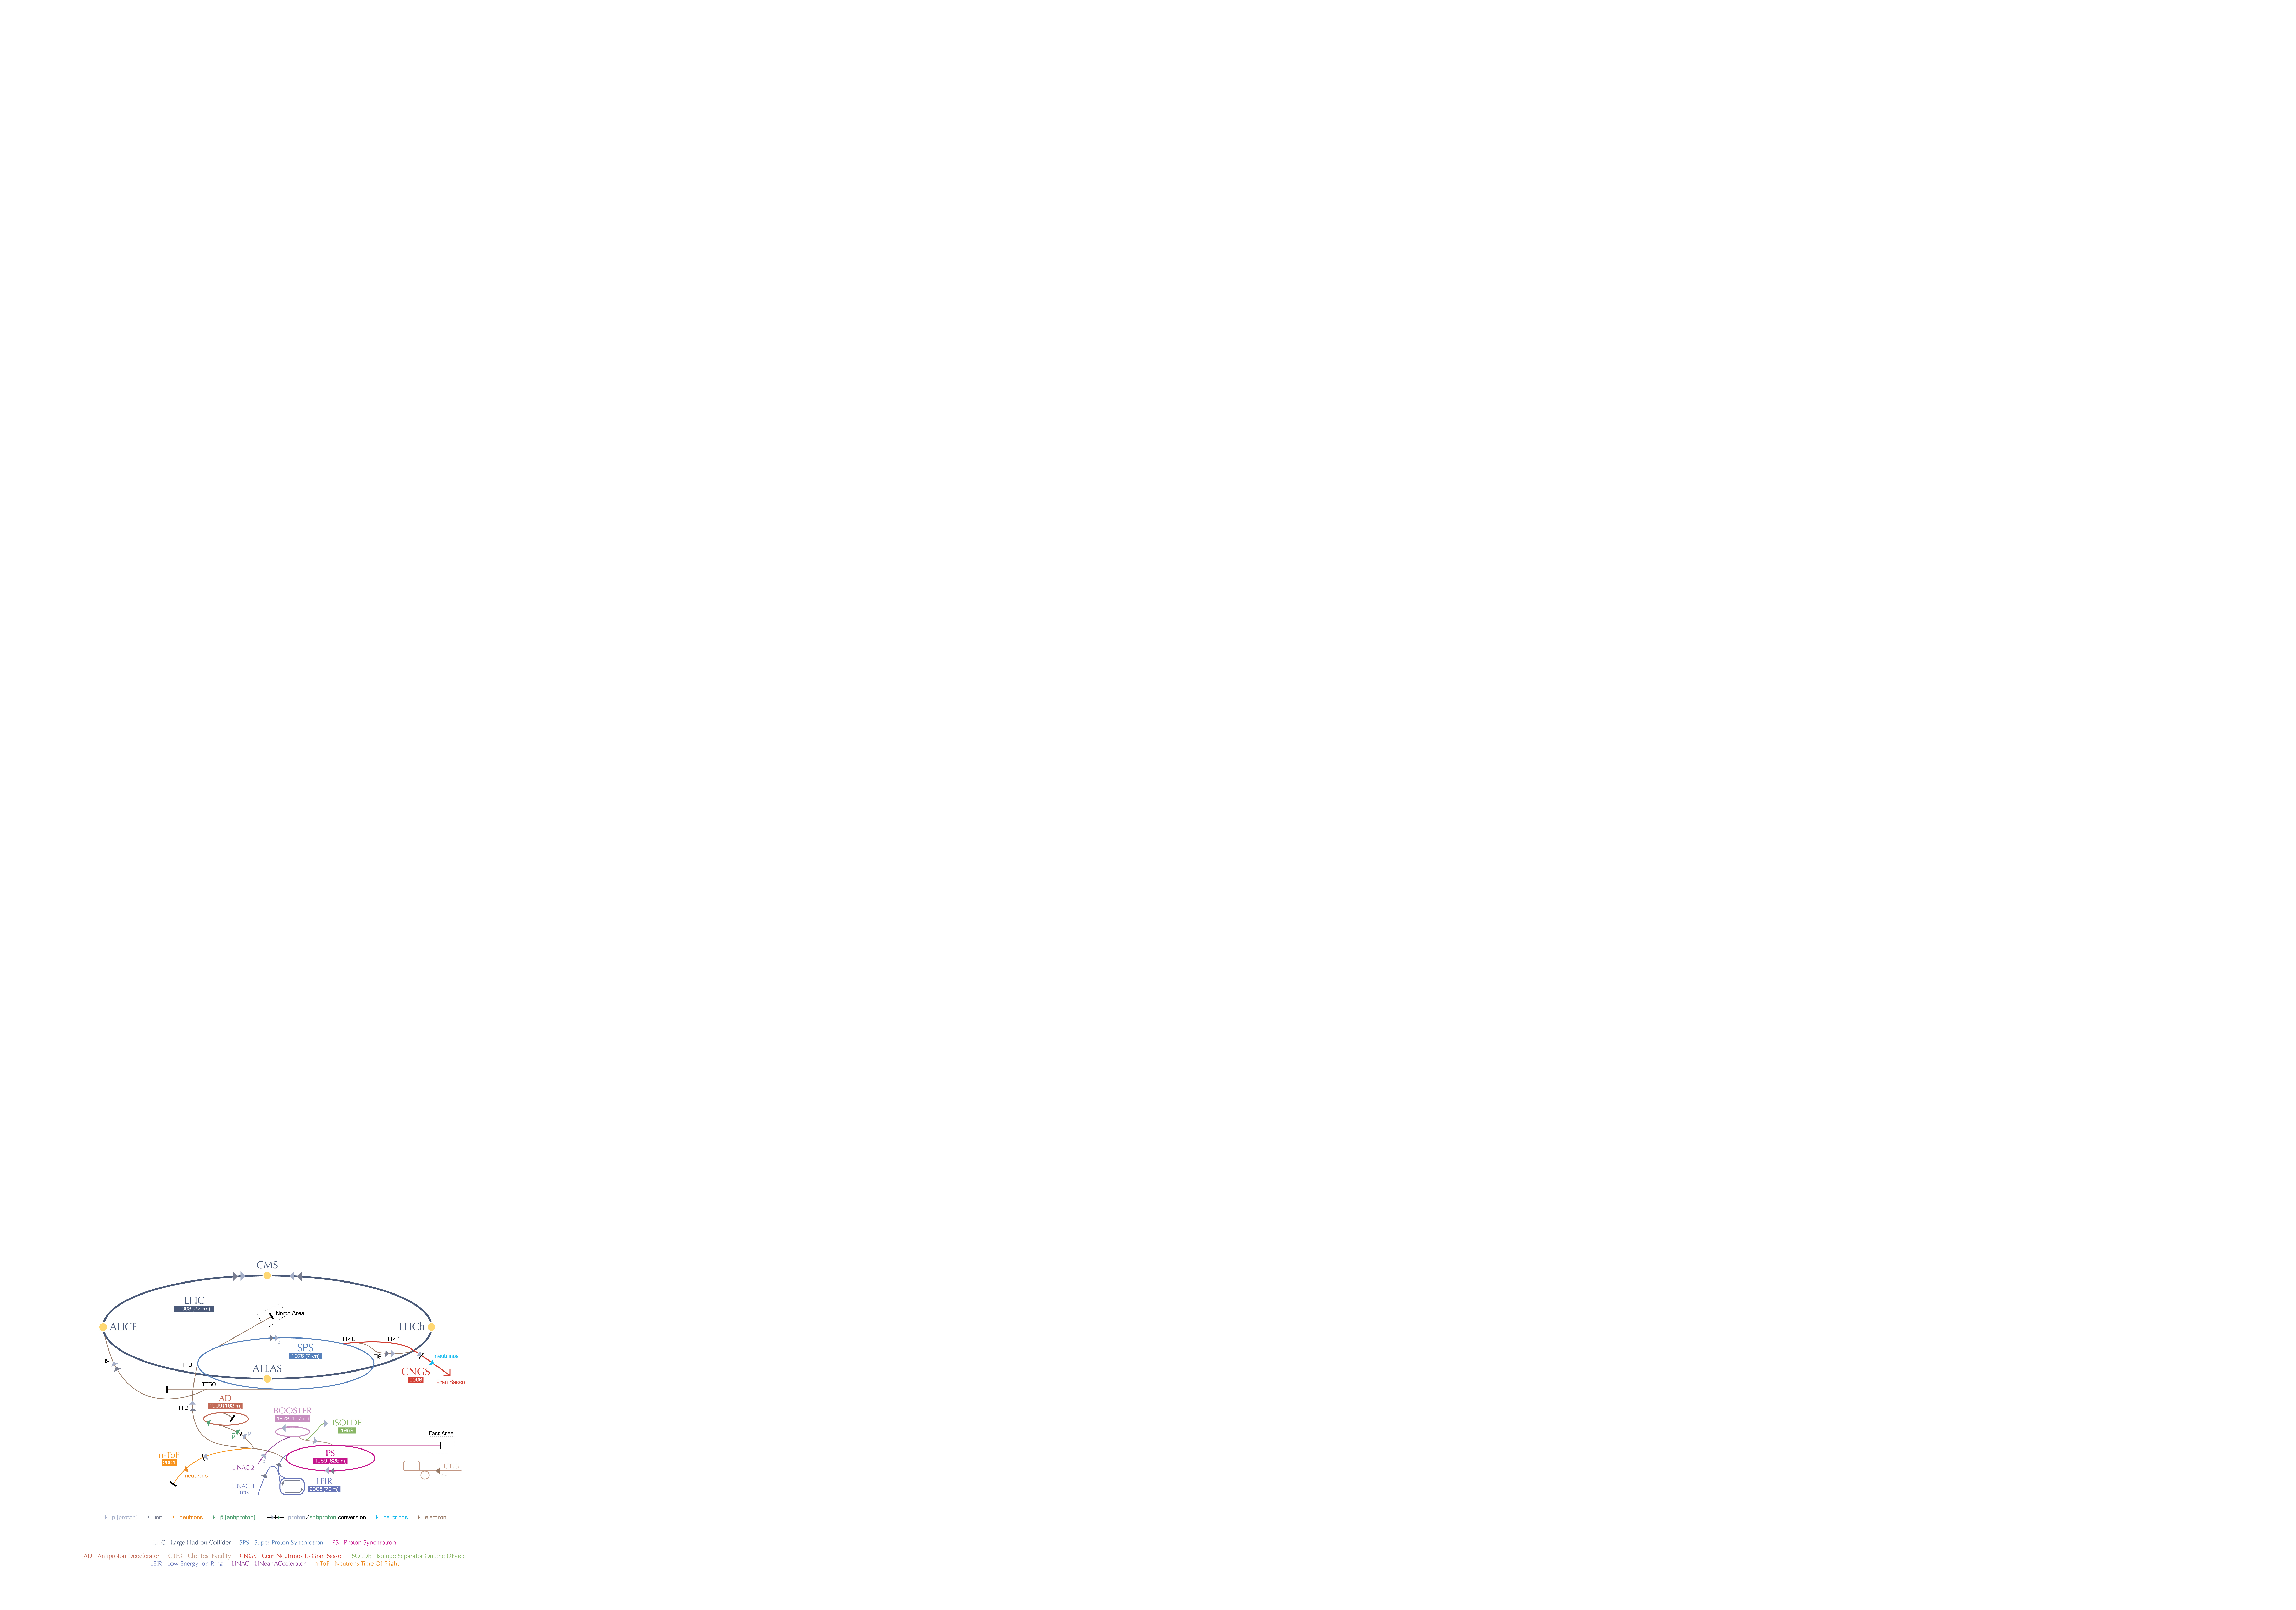
\includegraphics[width=\textwidth]{Figures/Detector/CERNschematic.pdf}
  \caption[The CERN accelerator complex.]
  {The LHC and its experiments within the CERN accelerator complex.
  Figure taken from Ref.~\cite{CERNcomplex}.}
  \label{fig:detector_CERNschematic}
\end{figure}

The LHC design parameters allow for proton-proton collisions to occur at a maximum centre-of-mass energy of 14\,TeV with an instantaneous luminosity of up to $10^{34}\,\textrm{cm}^{-2}\,\textrm{s}^{-1}$.
Prior to being injected into the LHC beam pipes, bunches of protons pass are accelerated in several stages. 
First, protons are obtained by stripping the electrons from hydrogen atoms using a strong electric field.
The protons produced are then accelerated up to an energy of 50 MeV by Linear Accelerator 2 (LINAC 2).
LINAC 2 leads into the Proton Synchrotron Booster (PSB), where they reach an energy of 1.4 GeV before passing into the Proton Synchrotron (PS).
Here the beam is accelerated up to 25 GeV before being transferred to the Super Proton Synchtroron (SPS).
The SPS is the last step before the protons enter the LHC itself at an energy of 540 GeV.
Therefore the LHC is responsible for the final acceleration from 540 GeV to the full energy.
Thus far, the energy reached for stable operation is 6.5\,TeV per beam; the full design energy is expected to be achieved in future.

The key components of the LHC are its 1232 main dipole magnets, 392 main quadrupole magnets and 16 radiofrequency (RF) cavities.
Superfluid helium cools the dipole magnets to 1.9K, at which temperature they produce the 8.3T magnetic field required to keep the beams in circular orbit.
Quadropole magnets are used principally to focus the beams near the interaction points, which increases the probability of a high-energy proton-proton collision.
The RF cavities deliver an accelerating field of 5MV/m at a frequency of 400MHz, and furthermore maintain the shape of the 2808 proton bunches per beam.
Collisions occur at the four interaction points, where bunches are induced to collide at a frequency of 25ns. 

The operation of the LHC to date has comprised two separate runs.
Run 1 commenced in 2010 with $\sqrt{s}$ = 7\,TeV, continuing into 2011 at the same centre-of-mass energy to give a total of 6.1\,\fb of data.
In 2012 this was increased to 8\,TeV, and a total of 23.3\,\fb of data were collected.
Analyses based upon this Run 1 dataset were able to discover the Higgs boson.
After a shutdown for upgrades to the machine, Run 2 ran from 2015 to 2018 at a constant 13\,TeV centre-of-mass energy.
The LHC was able to exceed its design luminosity in each of the years, eventually levelling the luminosity at $2\times10^{34}\,\textrm{cm}^{-2}\,\textrm{s}^{-1}$ for the majority of 2018 operations.
A number of additional inleastic proton-proton collisions in addition to a collision of interest, known as pileup, occur at a rate proportional to the instantaneous luminosity.
The mean number of pileup events was 27 per bunch crossing in 2016, and 37 in both 2017 and 2018 data-taking.
Figure \ref{fig:detector_Run1andRun2lumi} summarises the data collected in each year.
The latest \Hgg results on which this thesis is based have utilised the 2016 and 2017 datasets; 
plans for the final Run 2 result combining the 2016-2018 datasets are described in Chapter ~\ref{chap:conclusion}.
Furthermore, future upgrades to both the LHC and the CMS detector are discussed in Chapter~\ref{chap:hgcal}.

\begin{figure}[h!]
  \centering
  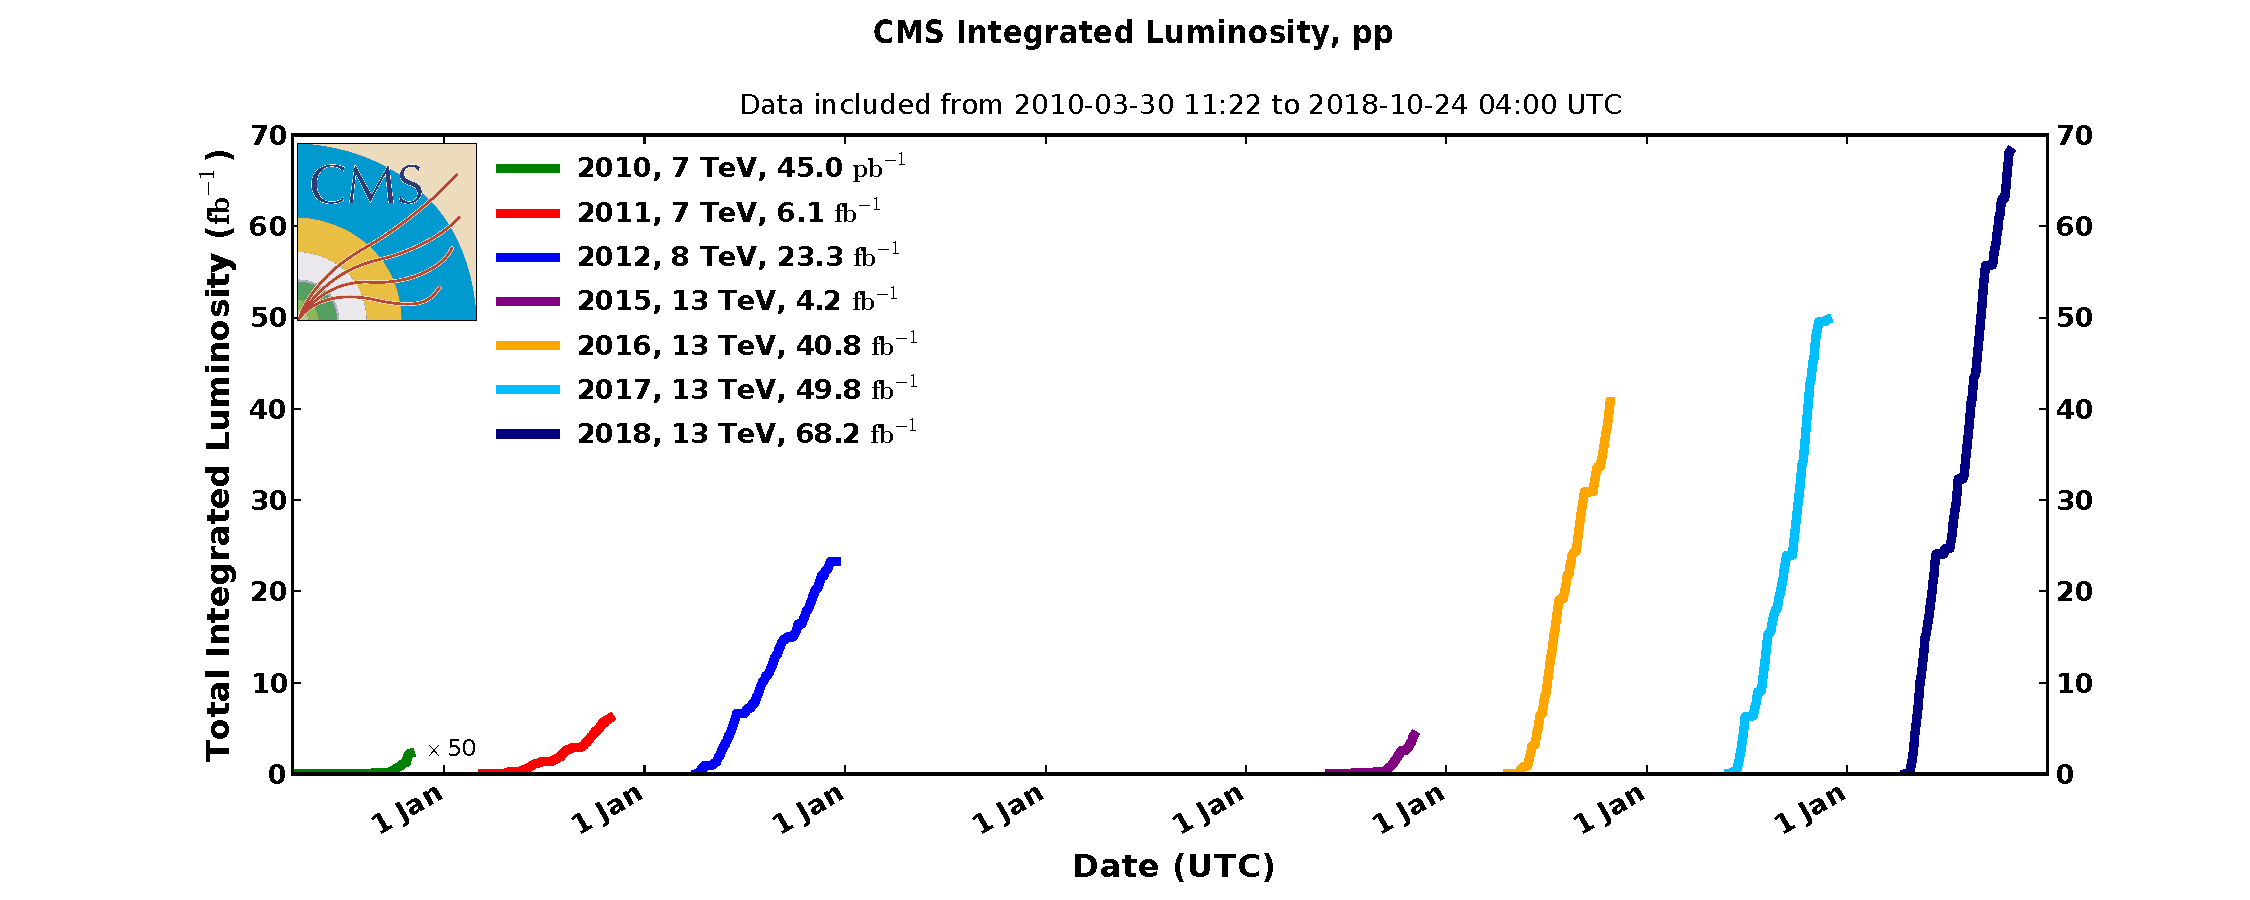
\includegraphics[width=\textwidth]{Figures/Detector/Run1andRun2lumi.pdf}
  \caption[LHC integrated luminosity and centre-of-mass energy per year.]
  {The integrated luminosity and centre-of-mass energy for each year of LHC operation.
  Figure taken from Ref.~\cite{CMSLumiPublic}.}
  \label{fig:detector_Run1andRun2lumi}
\end{figure}

\section{The CMS detector}

CMS is a general purpose detector~\cite{CMSdetector} designed to capture the full range of objects required to achieve the goals of the LHC physics programme.
The apparatus must be able to cope with very high pileup events at a very high rate; around 1000 charged particles are produced every 25\,ns.
Fine spatial and temporal granularity is required to obtain the sufficiently low occupancy necessary to perform well in these conditions.
The resulting quantity of detector channels presents challenges for the detector electronics.
Furthermore, the detector and its electronics must withstand high doses of radiation and fluence.

In addition to these technical constraints, CMS has four key physics requirements.
These are summarised as:
\begin{itemize}
  \item{\textbf{Muon identification and resolution} 
  muons must be identified and well-measured over wide range in energy and angle, 
  with good dimuon mass resolution and the capability to accurately determine their charge.}
  \item{\textbf{Charged particle measurement}
  good momentum resolution along with efficient reconstruction and triggering on $\tau$ particles and $b$-jets.}
  \item{\textbf{Electromagnetic energy resolution}
  good energy resolution and isolation for electrons and photons, whilst maintaining high acceptance.}
  \item{\textbf{Missing energy resolution}
  accurate missing energy calculation and mass resolution of dijet objects.}
\end{itemize}

The design of CMS fulfils each of these requirements.
The hermetic detector is cyclindrical in shape, housing the eponymous 4T solenoidal magnet in the central section.
Its other key components include the silicon tracker, homogeneous crystal electromagnetic calorimeter and a sampling hadronic calorimeter.
The tracker and calorimeters lie inside the bore of the magnet coil; the muon detection system is instead interleaved with the return yoke.
Each of these subsystems is displayed in Figure~\ref{fig:detector_CMSschematic}, and described in detail in the remainder of this chapter.

\begin{figure}[h!]
  \centering
  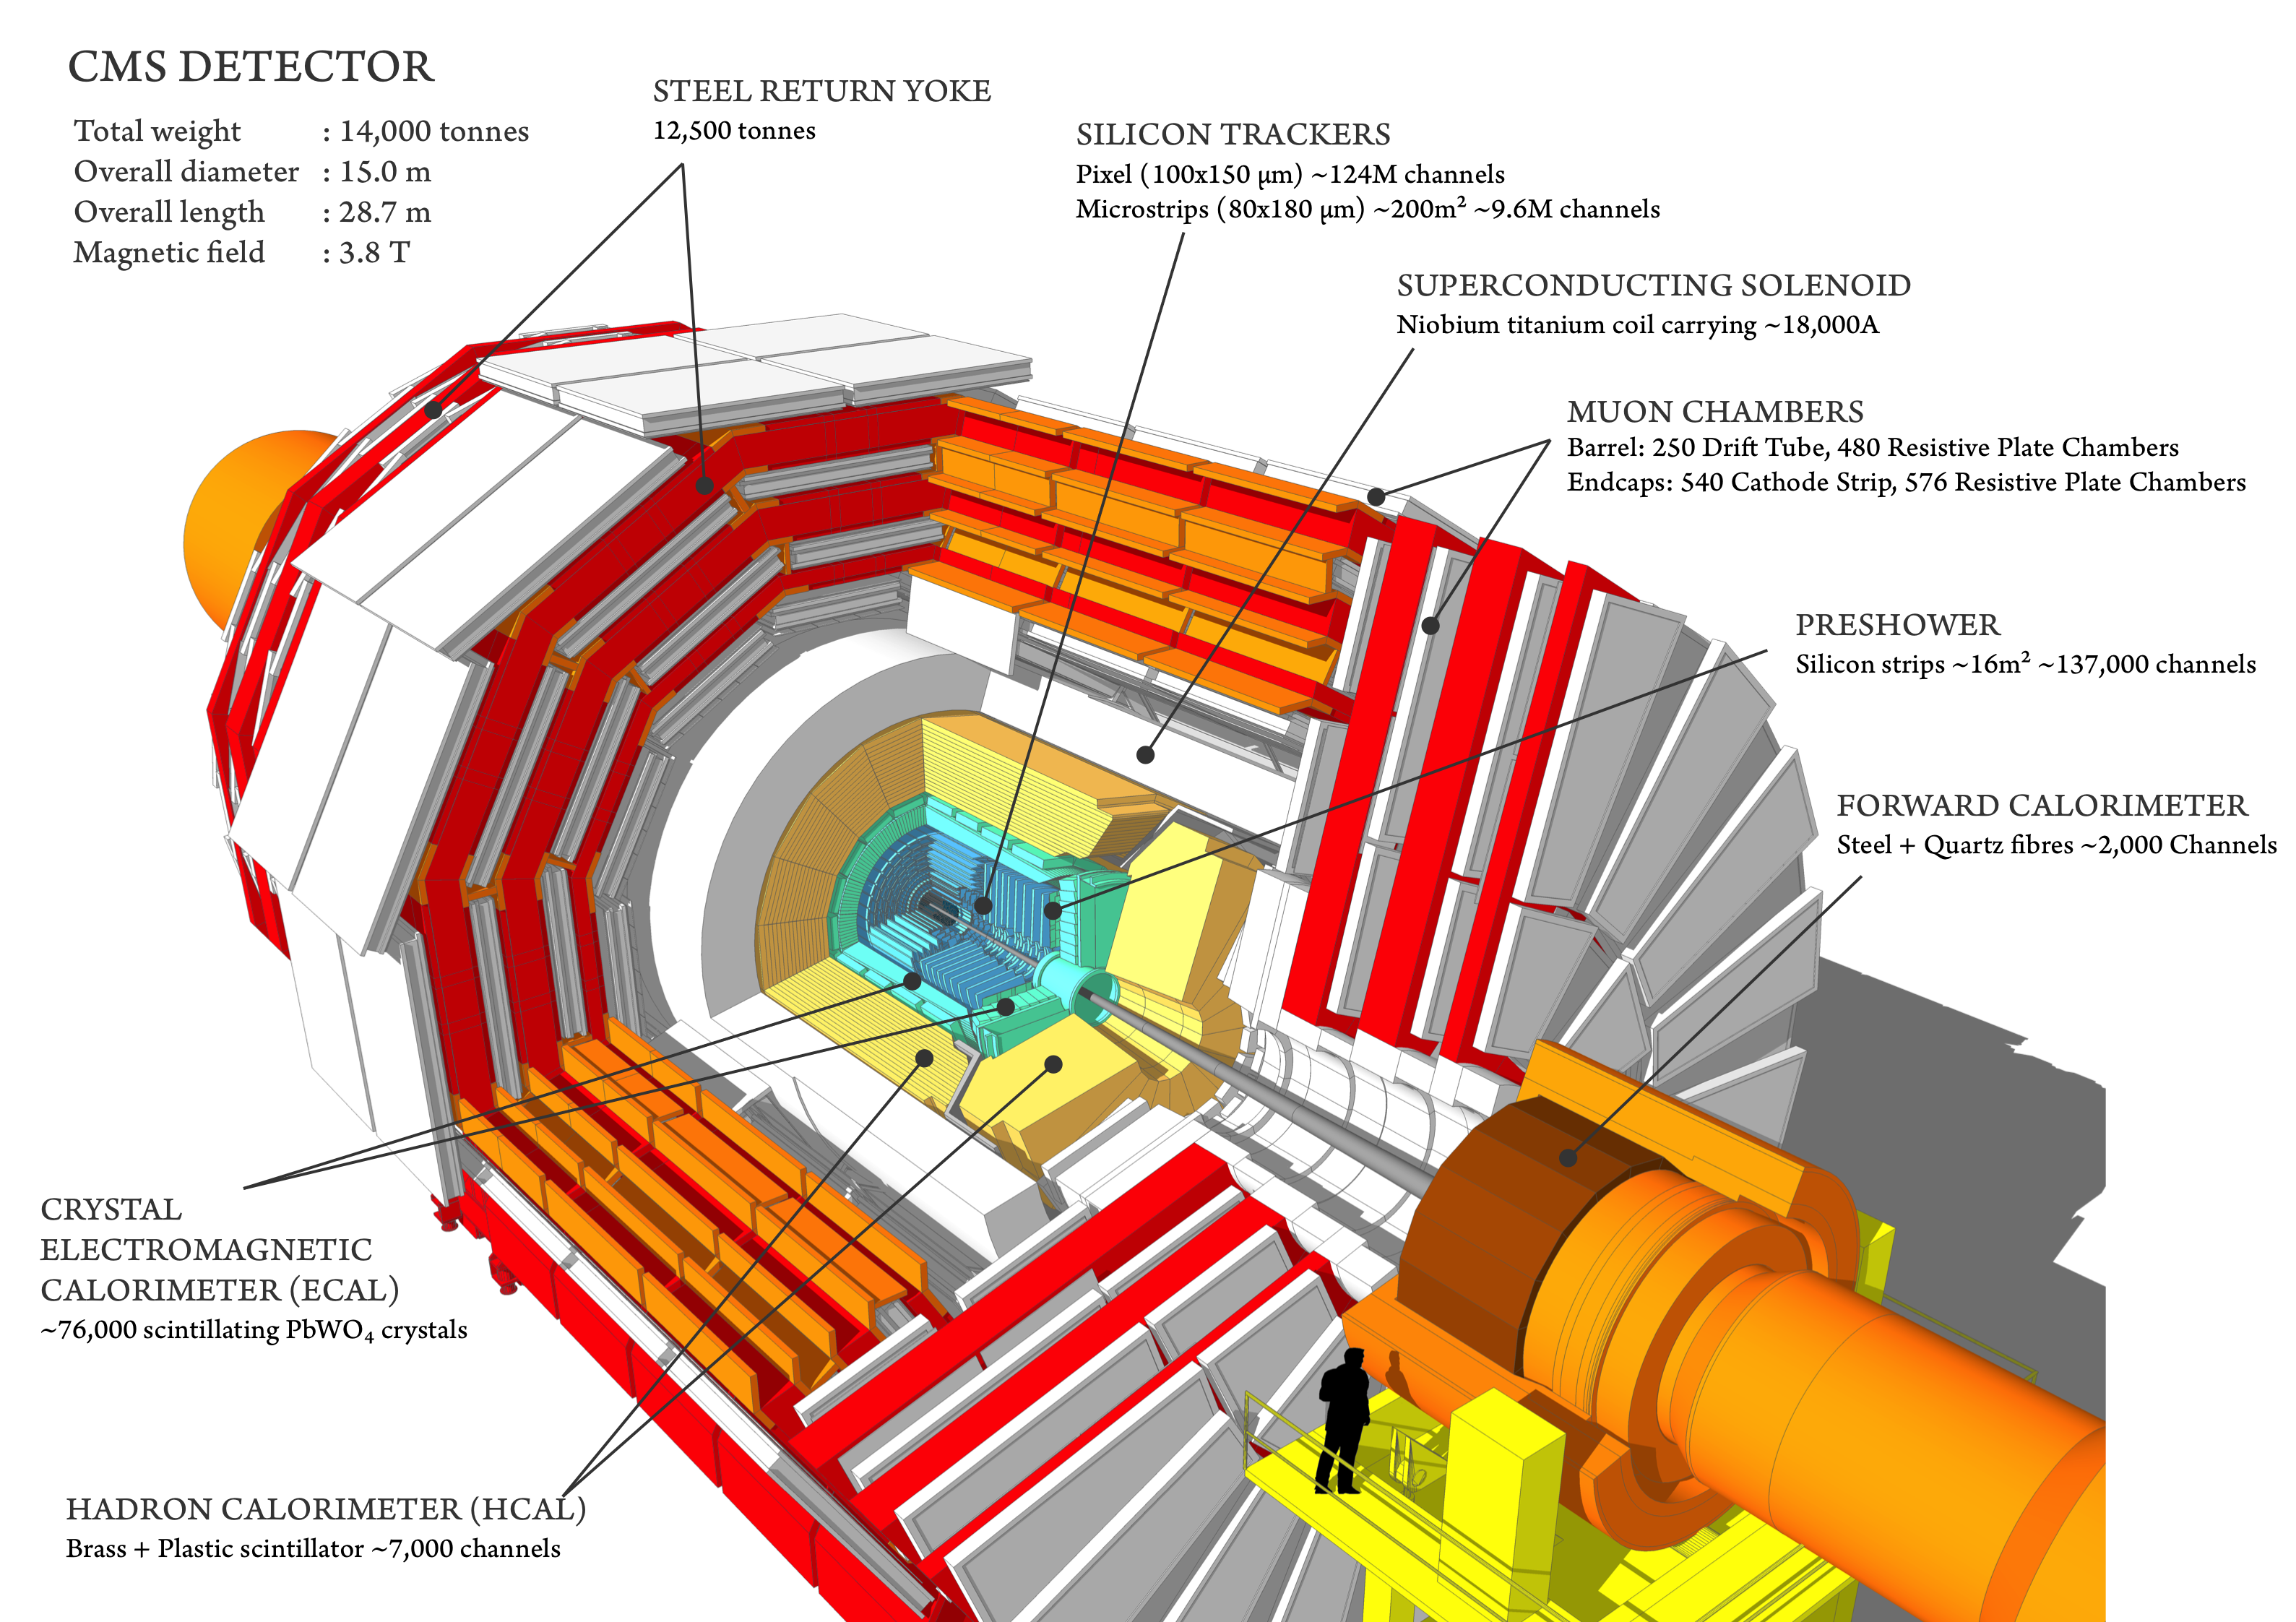
\includegraphics[width=\textwidth]{Figures/Detector/CMSschematic.png}
  \caption[A schematic view of CMS.]
  {A schematic view of the CMS detector.
  Part of the detector is cut away in order to display each subsystem.
  Figure taken from Ref.~\cite{SketchUp}.}
  \label{fig:detector_CMSschematic}
\end{figure}

A cylindrical cooordinate system is frequently used by CMS, with its centre at the nominal proton-proton interaction point.
The positive $z$-axis is defined to be parallel to the beampipe in the direction of the Jura mountains, anti-clockwise when viewed from above.
The azimuthal angle $\phi$ is measured from the $z$-axis, and polar angle $\theta$ from the plane perpendicular to the $z$-axis.
Other common quantities are: pseudorapidity, defined as $\eta = -\ln{\tan{\theta/2}}$; 
momentum in the direction transverse to the plane of the LHC, \pt; 
and the negative vector sum of particle energies, $E^{\textrm{miss}}_{T}$.

\subsection{Solenoid}
\subsection{Tracking}
\subsection{Electromagnetic calorimeter}
\subsection{Hadronic calorimeter}
\subsection{Muon system}
\subsection{Trigger system}

\chapter{The High Granularity Calorimeter}
\label{chap:hgcal}

\section{Introduction}
In order to fully exploit the physics potential of the LHC, 
the accelerator will be operated until around 2040 
in order to collect as much data as possible.
During this period, various upgrades are planned 
which are designed to maximise the instantaneous delivered to the experiments, including CMS.
As a result of this increase, and due to accumulated radiation damage, 
parts of the CMS detector will need to be upgraded.
A key part of this upgrade program is the replacement of the electromagnetic 
and hadronic calorimeter endcaps with the high granularity calorimeter (HGCAL).
In this chapter, the motivation for and design of the HGCAL is described.
The development of reconstruction software is detailed, 
and the detector's physics potential is demonstrated using the example of the VBF \Hgg analysis.

\section{The High Luminosity LHC}

Run~2 of the LHC is now complete, with over \SI{190}{\fbinv} of data delivered at $\sqrt{s}\,=\,\SI{13}{TeV}$. %original target was 150 Run 1 plus Run 2
This exceeds the original target of \SI{150}{\fbinv}, and was achieved partly because the machine was eventually operated at twice its nominal instantaneous luminosity.
The instantaneous luminosity reached values as high as \SI{2e34}{\lumi} during 2018.
The second long shutdown (LS2) commenced following the completion of Run~2 and will last until 2021.
During this time various improvements to the LHC will be made, including a substantial upgrade to the injection system.
The machine will also be readied for operation at the increased energy of \SI{7}{TeV} per beam.
However these upgrades will not substantially affect the conditions experienced by the LHC experiments; 
the peak instantaneous luminosity is not envisaged to increase beyond \SI{2e34}{\lumi}.
As such no major changes are required to the CMS detector during LS2, although various improvements are planned: 
these include upgrades to the muon system and HCAL barrel.
Therefore the expectation for Run~3, which commences in 2021 with two years of high-availability data-taking in 2022 and 2023, 
is that a further $\SI{150}{\fbinv}$ of data will be accumulated. 
%See here for details of LS2 and Run 3: https://indico.cern.ch/event/773482/contributions/3213751/attachments/1763994/2863045/LHC-Run2.CMS.Dec18.JW.pdf

Beyond Run~3, the usefulness of running the LHC with its current parameters decreases.
In order to reduce the statistical error on physics measurements by a factor of two, high-availability operation for more than ten years would be required.
Therefore a major upgrade to the LHC is planned, referred to as the Phase~2 upgrade, to maximise its physics reach. 
%insert info about what is actually being upgraded here? %TODO learn a bit about the things below 
%The technological innovations facilitating the upgrade include $\SI{12}{T}$ superconducting magnets, compact and precise superconducting cavities, and new beam collimation technology.
The resulting High~Luminosity~LHC (HL-LHC) \cite{HLLHC} will have a nominal levelled instantaneous luminosity of \SI{5e34}{\lumi}, 
permitting a total of \SI{3000}{\fbinv} of data to be collected by the mid-2030s.
The current planned schedule of the future running of the LHC and HL-LHC is summarised in Figure~\ref{fig:hgcal_LHCschedule}.

\begin{figure}[h!]
  \centering
  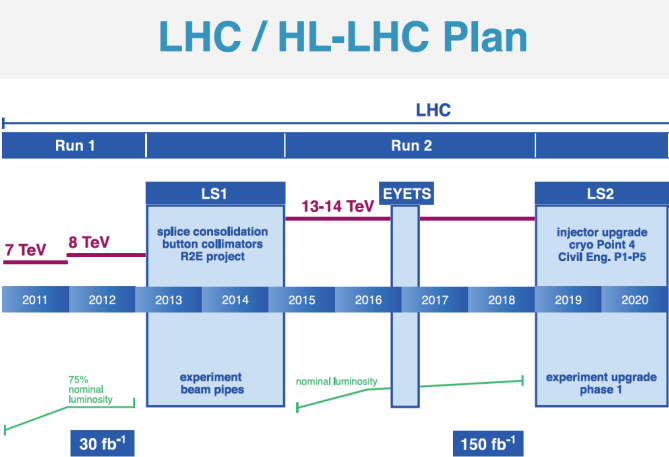
\includegraphics[width=0.8\textwidth]{Figures/HGCAL/LHCschedule1.png}
  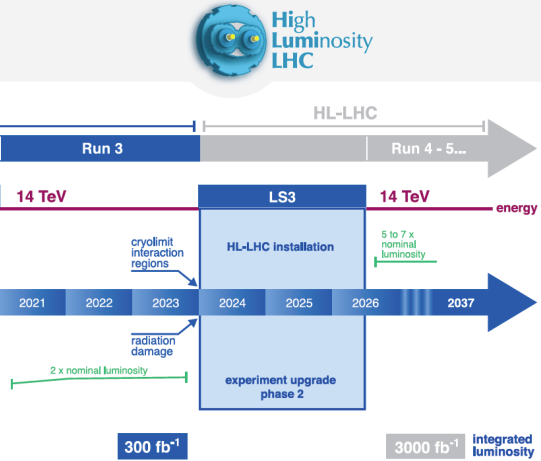
\includegraphics[width=0.8\textwidth]{Figures/HGCAL/LHCschedule2.png}
  \caption[Planned LHC and HL-LHC schedule.]
  {
    The planned schedule for the operation of the LHC and its high-luminosity upgrade.
    Figure taken from Ref.~\cite{FutureYR}.
  }
  \label{fig:hgcal_LHCschedule}
\end{figure}

\section{The CMS upgrade}

At the HL-LHC, the mean pileup per bunch crossing is expected to be 140; 
however an additional 50\% beyond the nominal value is allowed for in the HL-LHC design, 
which would result in mean pileup values of up to 200.
This constitutes a major change, and the environment will be significantly harsher than with the current LHC conditions.
These conditions pose serious challenges to the detectors in terms of radiation tolerance and reconstruction in high pileup.
In order to maintain or improve upon the excellent performance exhibited in Run~2, a suite of upgrades to the CMS detector are planned.
The key aspects of the CMS Phase~2 upgrade can be summarised as \cite{UpgradeTP,MTD}:
\begin{itemize}
  \item{\textbf{Tracker:}
  the tracker will suffer significant radiation damage and must be entirely replaced for Phase~2.
  The upgraded tracker will have finer granularity, %factor of 4
  increased coverage in the forward region, %up to eta=4
  and be much lighter, resulting in a reduced material budget.
  Furthermore, the design will allow track information to be included in the L1 trigger decision.}
  %enabling powerful background rejection at the earliest event selection step
  \item{\textbf{Endcap calorimeters:}
  the calorimeter endcaps (both ECAL and HCAL) will also be radiation-damaged by the end of Run~3, and will therefore be replaced.
  The replacement design, known as the high granularity calorimeter (HGCAL), will have both electromagnetic and hadronic sections.
  Fine segmentation in each of the longitudinal and transverse directions will facilitate precise measurements of showers in three dimensions.}
  \item{\textbf{ECAL barrel:}
  the current ECAL detector electronics are not capable of meeting the stringent HL-LHC trigger requirements.
  The level of noise in the silicon avalanch photodiodes which detect the scintillation light will also increase due to radiation damage.
  Therefore the electronics will be optimised and the operatimg temperature of the system reduced.} % from 18 to 8 degrees
  \item{\textbf{Timing:}
  precision timing measurements of objects will be made with the HGCAL and the upgraded ECAL.
  In addition, a dedicated timing layer providing precise timing information for minimum ionising particles will be added to the barrel and each of the endcaps.
  By enabling the reconstruction of vertex times, this will greatly improve the capability for pileup rejection.}
  \item{\textbf{Muon endcaps:}
  the CSC muon system will be enhanced with additional stations.
  This will increase the forward coverage and maintain muon acceptance at the L1 trigger.}
  %because new bits provide redundancy (only 1.5 to 2.4 doesn't have redundancy in muon system atm) and timing resolution.
  \item{\textbf{Trigger and data acquisition:}
  due to the tracker upgrade, the latency of the L1 trigger at Phase~2 is increased to \SI{12.5}{\micro\second}.
  Combined with upgrades to the front-end electronics of various subdetectors, %barrel calorimeter; the CSCs of the inner rings, and the DT readout.
  this enables an increase of the L1 trigger acceptance rate to \SI{500}{\kilo\hertz}.
  Consequently the data acquisition system must also be upgraded to handle the increase in event rate, event size, and the complexity of high PU reconstruction.}
\end{itemize}
Full details of the CMS upgrade scheme can be found in Refs~\cite{Tracker_Phase2TDR,Barrel_Phase2TDR,Muon_Phase2TDR,Trigger_Phase2TDR,DAQ_Phase2TDR,MTD,HGCAL}.
The remainder of this chapter is dedicated to describing the HGCAL in further detail, based upon Ref.~\cite{HGCAL}.

\section{Requirements for the HGCAL}

The primary challenge which drives the design of the HGCAL is the need to 
sustain physics performance in the extremely high pileup conditions foreseen at the HL-LHC.
Simulations indicate that the HGCAL will be required to withstand up to 2MGy of total radiation dose, 
together with a maximum fluence of around $\SI{10e16}{\textrm{n}_{\textrm{eq}}/\textrm{cm}^2}.$
The inhomogeneous distribution of this dose is shown in Figure~\ref{fig:hgcal_Dose}, 
which illustrates how the radiation dose is greatest near the beampipe.
Studies performed in recent years have shown that silicon sensors and the associated electronics 
retain acceptable performance after exposure to this level of radiation, 
and have hence been chosen as the most reliable active material for the majority of the calorimeter.
The remaining parts of the detector in lower-radiation regions will instead use 
cheaper plastic scintillator tiles with silicon photomultiplier (SiPMs) readout.
These layers of active material are interleaved with the copper-tungsten alloy absorber 
in the front section of the calorimeter, and stainless steel absorber further back.

\begin{figure}[h!]
  \centering
  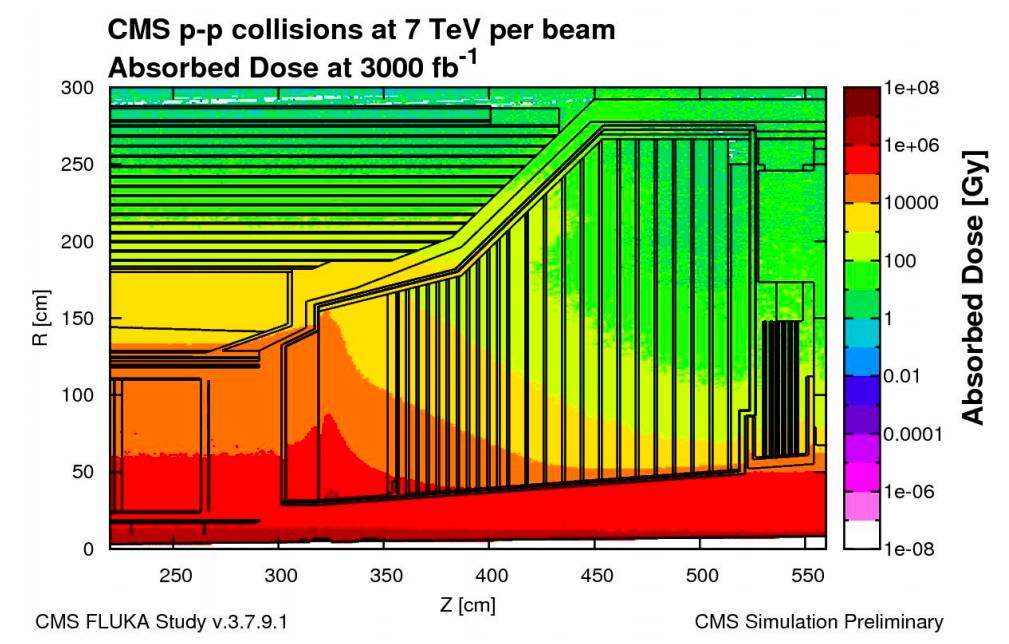
\includegraphics[width=0.9\textwidth]{Figures/HGCAL/Dose.png}
  \caption[Expected radiation dose for the HGCAL.]
  {
    The dosage of ionising radiation the HGCAL is expected to absorb 
    after a total integrated luminosity of \SI{3000}{\fbinv}, 
    as a function of detector radius and depth.
    The colour scale indicates the magnitude of the absorbed dose.
    Figure taken from \cite{HGCAL}.
  }
  \label{fig:hgcal_Dose}
\end{figure}

To maintain performance throughout the operation of the HL-LHC it is necessary 
to inter-calibrate cells to the level of a few percent.
This is possible provided the signal-to-noise ratio (S/N) 
for minimum-ionising particles (MIPs) is sufficiently high.
For this to be achieved after \SI{3000}{\fbinv} of data has been collected, 
small silicon cells with low capacitance are required, which results in high lateral granularity.
Fine lateral granularity also has many benefits for physics performance, 
including the ability to separate nearby showers, identify narrow jets 
such as those originating from the quarks produced in vector boson fusion (VBF) events, 
and minimise the amount of pileup entering energy measurements.
To take advantage of this fine segmentation the calorimeter is required to be dense, 
thereby preserving the compactness of showers in the transverse direction.
Similarly, fine longitudinal granularity facilitates precise energy measurements, 
as well as enabling discrimination between different types of shower using the depth profile.
These features are particularly important 
within the CMS particle flow reconstruction paradigm \cite{ParticleFlow}.
A detector producing three-dimensional images of showers would provide 
powerful separation of electromagnetic, charged hadronic and neutral hadronic components,
facilitating more precise energy measurements, particularly of jets.

In addition, the HGCAL should be able to perform precise timing measurements 
enabling excellent pileup rejection, and provide an input to the L1T decision.
The proposed design specification that captures all of these desired features 
is described in the following section.

\section{Design}

An overview of the HGCAL design is presented in Figure \ref{fig:hgcal_TheHGCAL}.
The HGCAL is composed of an electromagnetic and a hadronic section, called the CE-E and CE-H respectively, covering the pseudorapidity range $1.5\,<\,|\eta|\,<\,3.0$.
The CE-E comprises 28 layers with hexagonal silicon sensors as the active element.
The total depth, including the neutron moderator layer at the front, is \SI{34}{cm}, 
which corresponds to approximately 26 radiation lengths ($X_0$) 
and 1.7 interaction lengths ($\lambda$)
\footnote{A radiation length is defined as the mean distance over which 
a high energy electron will have its energy reduced to a fraction $e^{-1}$ of the initial value.}.
Three different thicknesses of silicon sensors are used, with thickness decreasing as a function of fluence.
Absorbers are made of copper-tungsten alloy and copper plates are used for cooling.
All layers of the CE-E are used for energy measurements, but alternate layers give inputs to the L1 trigger primitive formation. %TODO check why this is

The CE-H is formed of 12 layers with \SI{35}{mm} thick stainless steel absorber and another 12 where the absorber thickness is \SI{68}{mm}, contributing an additional \SI{9}{$\lambda$} in depth.
The active medium in the CE-H varies as a function of depth and radius, and is determined by the radiation level.
In regions of sufficiently low fluence (those which are nearest the back of the detector and furthest from the beam-pipe), plastic scintillator tiles are used with SiPM readout.
The exact threshold between the scintillator and silicon is determined by the S/N required to measure the MIP response, which is decreased by exposure to radiation.
Further detail on the design specifications of the HGCAL can be found in Ref.~\cite{HGCAL}.

\begin{figure}[h!]
  \centering
  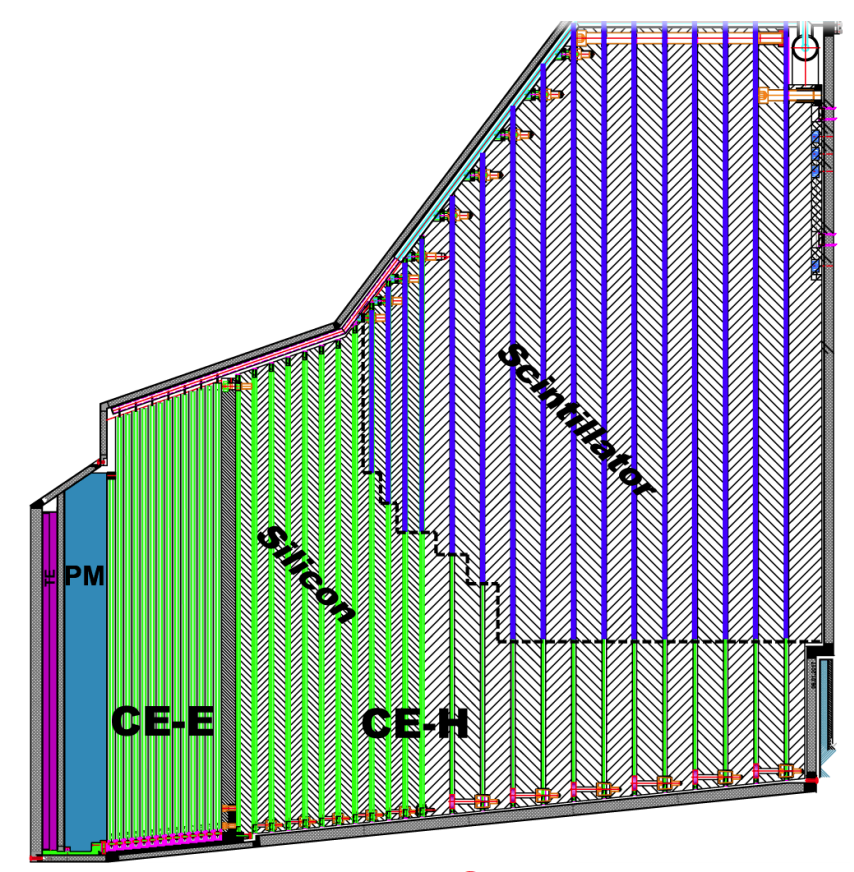
\includegraphics[width=0.8\textwidth]{Figures/HGCAL/TheHGCAL.png}
  \caption[Schematic of the HGCAL.]
  {
    A schematic of the HGCAL's longitudinal structure. 
    The endcap timing layer (TE, purple) is in the front of the HGCAL, 
    nearest to the nominal interaction point.
    A layer of polythene that moderates the flux of neutrons (PM, light blue) 
    also sits in front of the HGCAL.
    The actimve material of the electromagnetic part of the calorimeter (CE-E) 
    is entirely composed of silicon (green),
    whilst the hadronic part (CE-H) uses a mixture of silicon and plastic scintillator (dark blue)
    as active material.
    Adapted from \cite{HGCAL}.
  }
  \label{fig:hgcal_TheHGCAL}
\end{figure}

\section{Reconstruction}

\subsection{Electromagnetic objects} %TODO add more here, e.g. Artur's plots?

The HGCAL's intrinsic performance measuring the energy of electromagnetic showers 
is modelled using a dedicated simulation 
with pileup corresponding to an average of 200 interactions per bunch crossing. %TODO intrinsic performance means...
Energy deposits in a radius of \SI{26}{mm} around a single unconverted photon 
are summed to estimate the energy resolution, 
which is shown in Figure \ref{fig:hgcal_PhotonReso}. %TODO justify 26mm value
The left plot shows that the resolution is approximately constant as a function of $\eta$, 
and robust against pileup, with only a very small degradation in resolution between PU 0 and PU 200. %this is achieved due to the fine granularity
This intrinsic performance is further demonstrated 
by using this method to reconstruct unconverted photon pairs from simulated \Hgg decays, 
where both photons are contained within the fiducial region of the HGCAL 
and the vertex location is assumed to be known exactly. 
The resulting diphoton mass distribution is shown in Figure \ref{fig:hgcal_DiphotonReso}, 
with resolution of around \SI{1.8}{GeV}.
This value is comparable to the expected resolution of the upgraded CMS barrel calorimeter, 
representing a substantial improvement relative to Run 2, 
where the endcap resolution is significantly worse than the barrel. %TODO quantify this

\begin{figure}[h!]
  \centering
  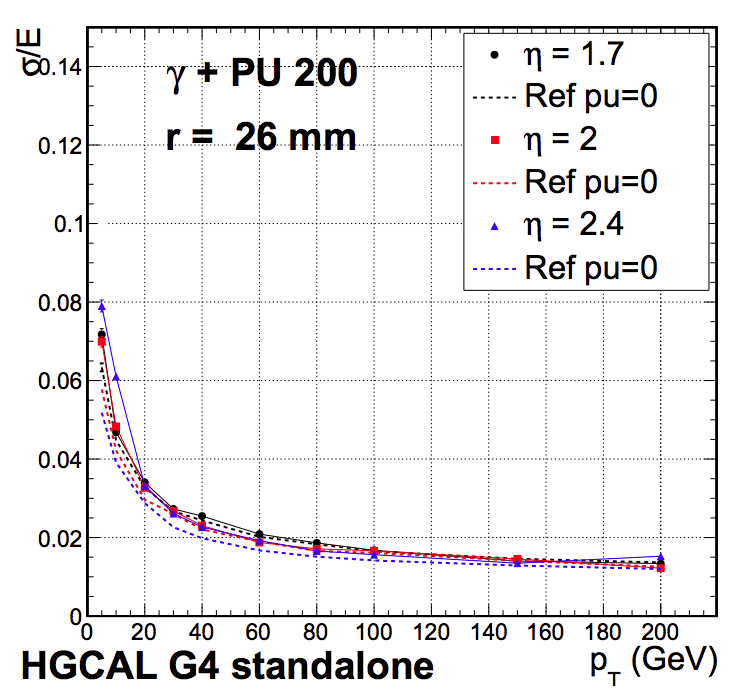
\includegraphics[width=0.6\textwidth]{Figures/HGCAL/SinglePhotonReso.png}
  \caption[HGCAL photon energy resolution.]
  {
    The intrinsic energy resolution for single photons in PU 200. 
    The energy is estimated by summing all deposits within a \SI{26}{mm} radius 
    of the generated particle axis. 
    Figure first shown in from Ref.~\cite{HGCAL}.
  }
  \label{fig:hgcal_PhotonReso}
\end{figure}

\begin{figure}[h!]
  \centering
  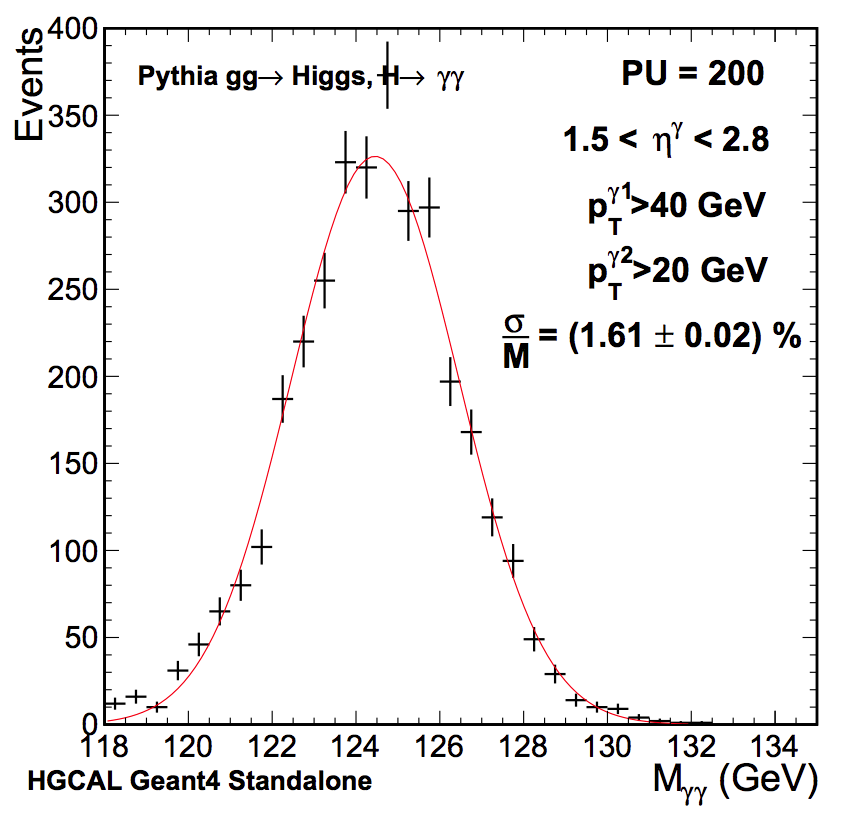
\includegraphics[width=0.6\textwidth]{Figures/HGCAL/HggReso.png}
  \caption[HGCAL diphoton mass resolution.]
  {
    The intrinsic diphoton mass resolution of the HGCAL in simulated \Hgg events 
    where both photons are within the fiducial region of the HGCAL. 
    Figure taken from Ref.~\cite{HGCAL}.
  }
  \label{fig:hgcal_DiphotonReso}
\end{figure}

The HGCAL provides more detailed shower information than existing CMS detectors, 
and it is envisaged that eventually a sophisticated four-dimensional particle flow approach will be used to incorporate as much of this information as possible. 
In the meantime, more straightforward approaches to reconstruction have been developed, 
in order to understand which approaches are feasible and to produce object and physics-level results that demonstrate the potential of the detector. 

%Furthermore, no use is yet made of the intrinsic timing capabilities of the silicon sensors, which will be invaluable in reducing the amount of out-of-time pileup at the HL-LHC. 
The current method begins by clustering hits in each two-dimensional (2D) layer independently, using an imaging algorithm \cite{ClusteringAlgo}.
The algorithm proceeds as follows, and is illustrated in Figure~\ref{fig:hgcal_clustering}:
\begin{enumerate}
  \item Construct an energy density map of all hits above a threshold $E_c$. 
  The threshold value is defined as a function of the noise resolution ($\sigma_{\textrm{noise}}$), which depends on the cell type.
  The density is defined simply as the energy sum of all hits within a critical distance $\delta_c$, 
  whose value is chosen to be similar to the Moli\`ere radius 
  \footnote{}. 
  \item For each hit, calculate the distance to the nearest hit with higher density.
  \item Assign hits with both both density and distance parameters greater than threshold values as cluster centres.
  The density threshold ($\rho_c$) can be defined relative to the maximum density in the event,
  or as a function of the noise resolution.
  The distance threshold is equal to $\delta_c$.
  \item Form clusters by assigning each hit to the same cluster as the nearest hit with higher density.
\end{enumerate}

\begin{figure}[h!]
  \centering
  \begin{subfigure}{0.292\textwidth}
    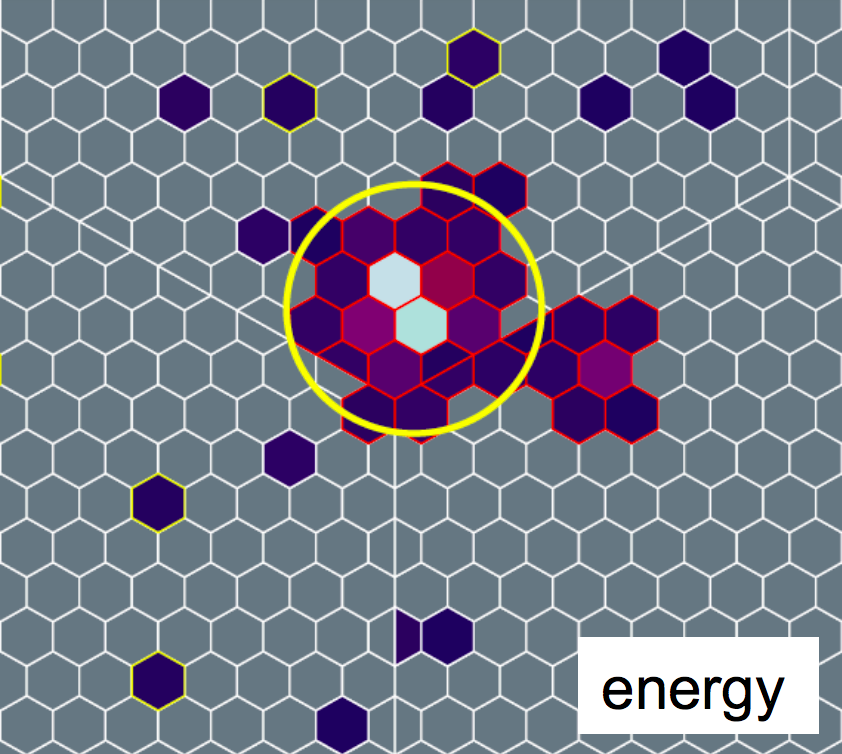
\includegraphics[width=\textwidth]{Figures/HGCAL/ClusteringAlgo_Energy.png}
    \caption{Energy}
  \end{subfigure}
  \begin{subfigure}{0.292\textwidth}
    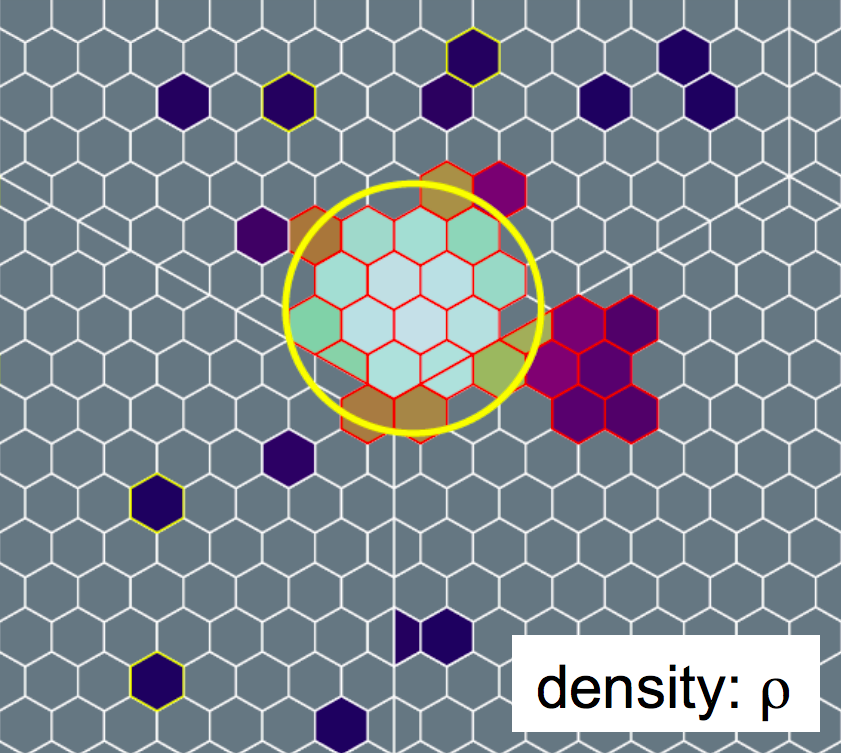
\includegraphics[width=\textwidth]{Figures/HGCAL/ClusteringAlgo_Density.png}
    \caption{Density, $\rho$.}
  \end{subfigure}
  \begin{subfigure}{0.3\textwidth}
    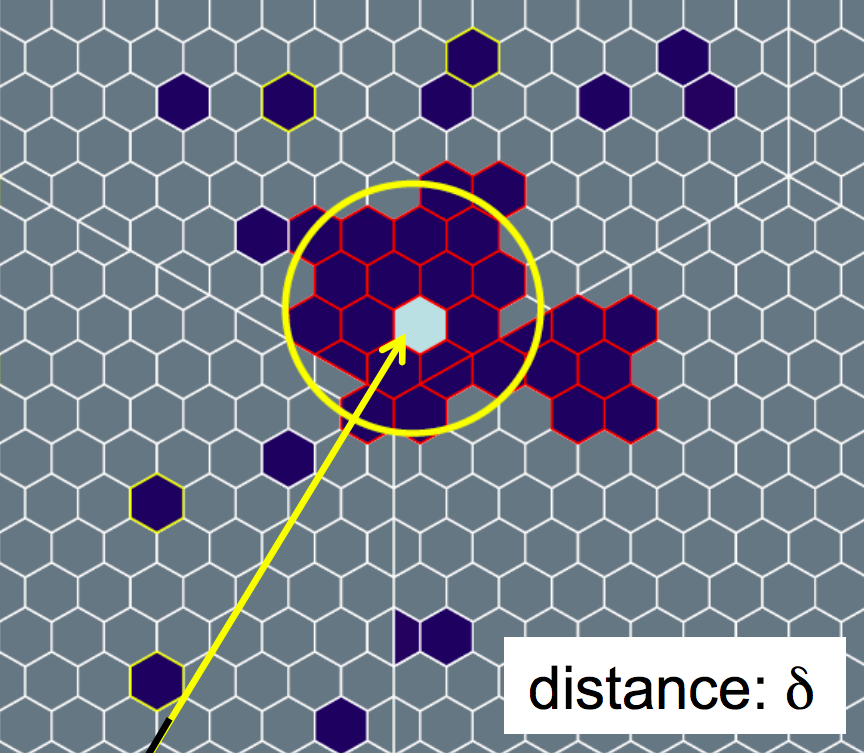
\includegraphics[width=\textwidth]{Figures/HGCAL/ClusteringAlgo_Distance.png}
    \caption{Distance, $\delta$.}
  \end{subfigure}
  \caption[Illustration of the imagine algorithm used for HGCAL layer clustering.]
  {
    Illustration of the procedure used to form layer clusters for electromagnetic objects in the HGCAL.
    The event considered is a single photon with $\pt\,=\,\SI{35}{GeV}$.
    The colour scale represents only the difference between hits, and is in arbitrary units.
    The yellow circle indicates the size of the Moli\`ere radius
    and the yellow arrow points to the hit chosen as a cluster centre.
    It can be seen that many hits in a genuine cluster have a high density, 
    whereas all but one will have a low distance to the nearest higher energy hit;
    requiring high values of both these parameters is therefore an appropriate way to define a cluster.
  }
  \label{fig:hgcal_clustering}
\end{figure}

There are therefore several parameters in the process which can be optimised: $E_c$, $\delta_c$, and $\rho_c$.
To form a suitable object on which to optimise, a more realistic object must be formed.
Therefore the 2D clusters, or layer clusters, produced are associated together in depth to form so-called multiclusters. 
An axis is defined by the highest energy 2D cluster, then any layer clusters within a certain distance of this axis are added to the multicluster.
Using this procedure with sensible parameters, an unconverted photon will have almost all of its energy contained within a single multicluster.
Optimisation can then be performed by minimising the energy resolution of unconverted photons simulated at a range of \pt values.
%It is anticipated that this two-step process could be improved by performing 3D clustering directly, but this remains to be studied in detail. 

Finally, electromagnetic objects are formed using a superclustering procedure very similar to the one utilised in Run 2, 
where showers which have been spread out in the $\phi$ direction by the magnetic field are collected together.
To perform this step, multiclusters are used as inputs to the existing Run~2 algorithm~\cite{PhotonReco}; no re-optimisation is performed.
Despite this, high \pt photons reconstructed in this way in have a resolution of below 2\%, 
not far from the intrinsic resolution values shown in Figure~\ref{fig:hgcal_PhotonReso}.
This method of electromagnetic object reconstruction was used for all the physics results in Ref~\cite{HGCAL}, 
including the study described in Section\ref{sec:hgcal_physics}.

Electrons defined in this way are used to test the ability of the HGCAL 
to discriminate between signal (\Zee) and background (QCD multijet) processes. 
Lateral and longitudinal shower shape variables, 
along with tracking information, are used as inputs to a BDT classifier. 
Two examples are shown in Figure~\ref{fig:hgcal_electronID}: 
the longitudinal development of the shower is indicated by the layer 
at which 10\% of the total energy in the CE-E has been deposited, 
and the lateral spread of the shower evaluated using the pseudorapidity difference 
between the electron multicluster and the extrapolated track.
For both variables, the distributions are robust to the increase in pileup 
and show good discrimination between the signal and background processes.
For a 95\% signal efficiency, the background efficiency is 1\% 
for electrons with $\pt\,>\,\SI{20}{GeV}$, comparable to the Run 2 value. %TODO check Run 2 value
An improvement in performance is seen when the lateral and longitudinal shape variables 
are added to a classifier using solely track information, 
demonstrating the value of the HGCAL granularity to the object identification.

\begin{figure}[h!]
  \centering
  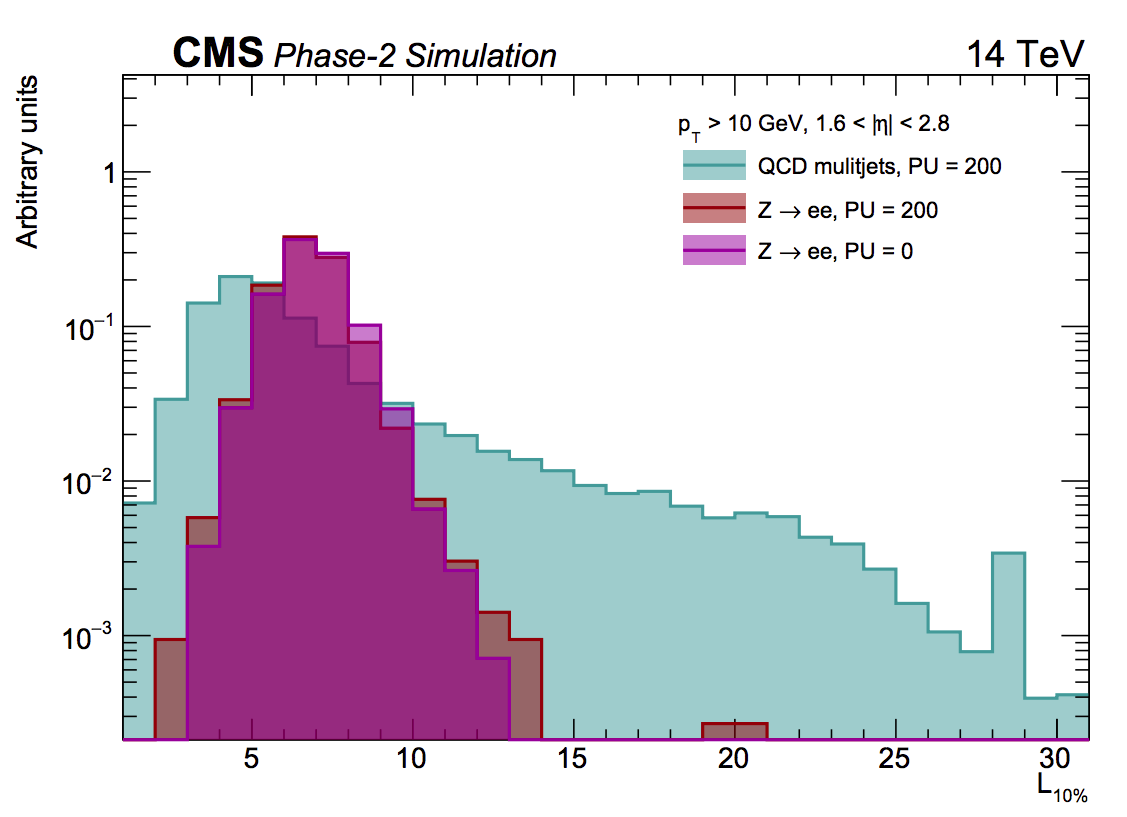
\includegraphics[width=0.7\textwidth]{Figures/HGCAL/electronIDlon.png}
  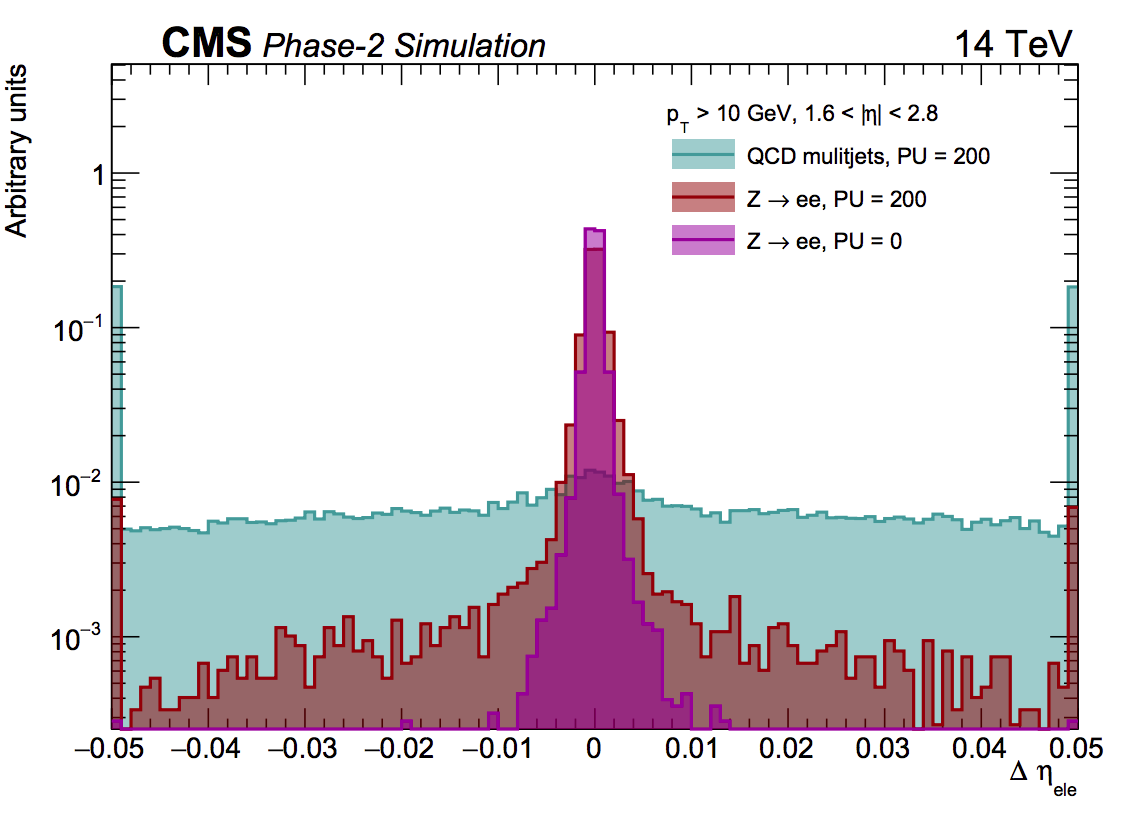
\includegraphics[width=0.7\textwidth]{Figures/HGCAL/electronIDlat.png}
  \caption[Distributions of electron shower shape variables.]
  {
    Shower shape variables used for electron identification.
    The longitudinal development of the shower is indicated by the upper plot, 
    which shows the layer at which 10\% of the total energy in the CE-E is deposited.
    The lower plot shows the pseudorapidity difference between the electron multicluster
    and the extrapolated electron track, which is a measure of the lateral spread of the shower.
    Figures taken from Ref.~\cite{HGCAL}.
  }
  \label{fig:hgcal_electronID}
\end{figure}

\subsection{Hadronic objects}

The multiclustering procedure is not found to work sufficiently well for hadronic showers.
This is due to the fact that hadronic showers are less well-contained, and also have more variation in transverse and longitudinal structure than electromagnetic showers.
Instead, single hadrons were reconstructed using a so-called megaclustering procedure, where layer clusters within a truncated cone are combined to form the object. 
For these more dispersed hadronic showers, the resolution substantially improves once the contribution of pileup is subtracted.
The pileup subtraction was implemented by removing the total energy of a similar cone randomly rotated in $\phi$. 
The energy resolution for a single pion with $\pt\,=\,\SI{25}{GeV}$ before and after the subtraction is shown in Figure \ref{fig:hgcal_SingleMegacluster}. 
The megaclustering algorithm is shown to yield adequate energy resolution of around 20\%. 
It is also robust against pileup; Figure~\ref{fig:hgcal_MegaclusterVsPt} shows the modest worsening between PU 0 and PU 200 that decreases quickly as a function of \pt.
This method of reconstruction is not yet incorporated in the central CMS reconstruction software.
For the physics results in Ref~\cite{HGCAL}, a realistic truth-information-driven approach was instead used for hadronic objects.

\begin{figure}[h!]
  \centering
  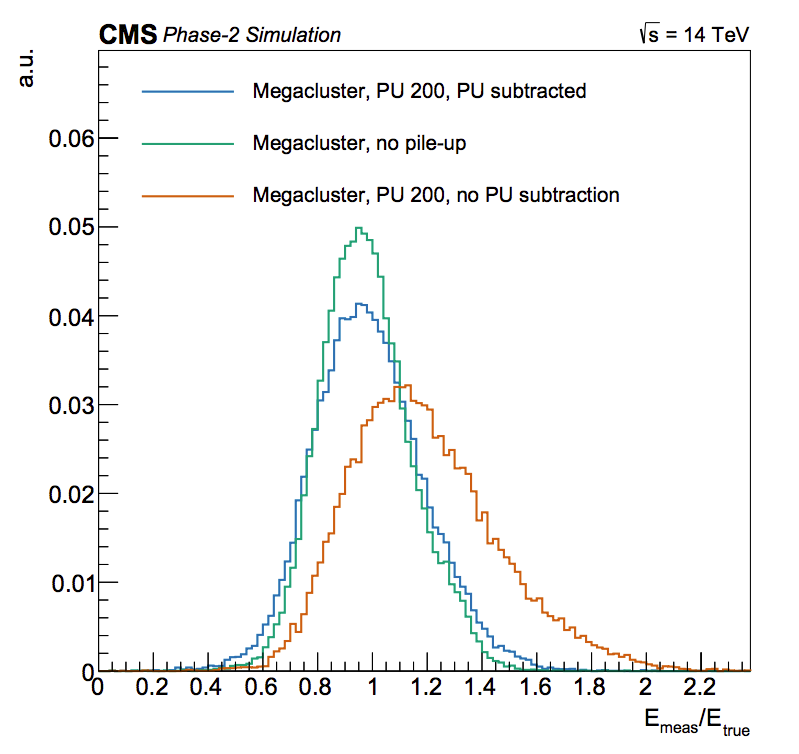
\includegraphics[width=0.65\textwidth]{Figures/HGCAL/SingleMegacluster.png}
  \caption[HGCAL pion energy response.]
  {
    The distribution of the energy resolution for single $\pt\,=\,\SI{25}{GeV}$ pions 
    reconstructed using the megaclustering algorithm, 
    before and after pileup subtraction. 
    Figure taken from Ref.~\cite{HGCAL}.
  }
  \label{fig:hgcal_SingleMegacluster}
\end{figure}

\begin{figure}[h!]
  \centering
  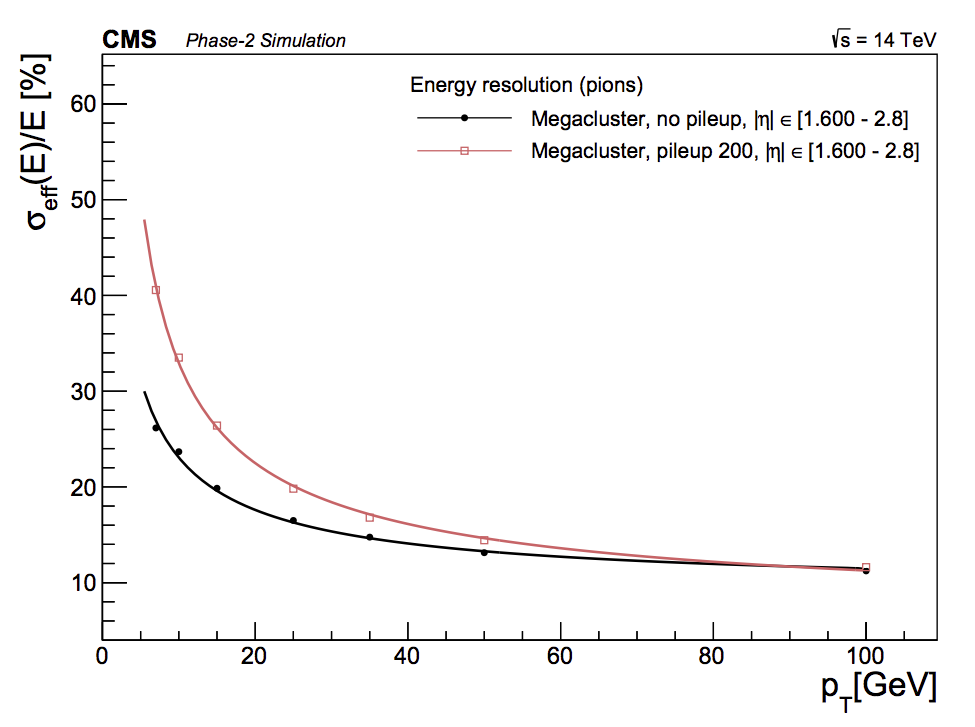
\includegraphics[width=0.7\textwidth]{Figures/HGCAL/MegaclusterVsPt.png}
  \caption[HGCAL pion energy resolution as a function of \pt.]
  {
    The mean energy resolution for single $\pt\,=\,\SI{25}{GeV}$ pions 
    reconstructed using the megaclustering algorithm, after pileup subtraction, 
    as a function of \pt. 
    Figure taken from Ref.~\cite{HGCAL}.
  }
  \label{fig:hgcal_MegaclusterVsPt}
\end{figure}

\subsection{Future development}
The reconstruction methods described above are preliminary and designed only to show the potential performance of the HGCAL subdetector.
There are a wide range of possibilities that will be explored before the eventual installation of the HGCAL.
Firstly, it is possible to extend the 2D clustering algorithm to three dimensions, enabling the construction of multicluster-like objects in one step.
This could potentially improve performance by including correlations between layers and including the longitudinal shower shape, 
rather than treating each layer as independent.
Furthermore, the image-like data produced by the HGCAL is well-suited to the use of machine learning algorithms, particularly those based on neural networks (NNs).
It is likely that eventually the initial pattern recognition step identifying showers will use NNs, and this is already under study.

Secondly, as mentioned above, the CMS particle flow algorithm has not yet been optimised to include all of the new information provided by the upgraded detector.
So far all studies have focussed on the calorimeter system alone; dedicated integration of tracking information, 
probably with an iterative approach, will bring substantial improvements.
This has already been demonstrated by the effectiveness of the particle flow approach in Runs~1 and 2~\cite{ParticleFlow}.

Finally, there is the exciting possibility of performing event reconstruction in four dimensions using timing information.
Both the upgraded ECAL and the HGCAL will provide precise timing information for showers, 
which will be used both for rejecting out-of-time pileup and for the separation of overlapping and adjacent showers.
In addition, the timing information from the MIP timing detector brings many new possibilities. 
It enables the four-dimensional reconstruction of vertices and tracks, 
which has already been shown to improve the vertex identification in \Hgg events at PU 200 from 40\% to 80\% \cite{MTD}.
The added benefit of fully integrating the timing information into the particle flow algorithm in a coherent way remains to be seen.

\section{Physics performance in the \Hgg decay channel}
\label{sec:hgcal_physics}
The performance of the HGCAL and the reconstruction techniques developed for its use 
are tested by evaluating their impact on CMS physics analyses.
In this section, a study of the impact on the CMS \Hgg analysis is described;
the diphoton channel will continue to be very important for characterising the Higgs boson's 
properties at the HL-LHC.
Rather than repeating the analysis in full, 
specific aspects of the analysis which will be affected by the HGCAL upgrade are investigated.

In Run 2, the sensitivity of the \Hgg analysis is driven by barrel-barrel diphoton pairs.
The effect of the HGCAL greater acceptance (to $|\eta|=3$) relative to the current ECAL endcaps
(to $|\eta|=2.5$) is to increase the number of available diphotons by approximately 12\%.
Furthermore, the diphoton mass resolution in the endcap is found to be very similar 
to that in the barrel.
This is an improvement upon the Run~2 endcap, 
which has significantly worse resolution than the barrel, 
and also increases the usefulness of the increased forward acceptance.

A more substantial benefit of the HGCAL upgrade 
will be the ability to separate quark-initiated jets from jets which originate from gluon emission.
This is illustrated in a study of the ggH and VBF production modes in the \Hgg decay channel, 
using events simulated under HL-LHC conditions with the upgraded CMS detector.
In the Run~2 analysis, the so-called dijet BDT is used to discriminate between ggH and VBF
using photon and jet kinematic variables.
Here, the possibility of exploiting the granularity of the HGCAL 
by using jet shape variables as BDT inputs in addition to the kinematic variables is explored.

Jets initiated by gluons tend to have lower \pt values and be more dispersed than quark-initiated jets, 
which are relatively highly collimated and contain fewer particles. 
Therefore variables relating to the jet shapes can be used to discriminate between the two.
Since jets in ggH events tend to be gluon-initiated, 
and the VBF jets quark-initiatied, 
this can in turn provide discrimination between the two production processes.

The impact of the HGCAL is evaluated by comparing the performance of two different BDTs.
Three jet shape variables are used to construct a BDT referred to as the jet shape BDT.
A second BDT, known as the dijet BDT, uses additional kinematic variables including those of the photons; 
its inputs are identical to the dijet BDT used in the Run~2 analysis 
(see Chapter~\ref{chap:categorisation} for details), but with the three jet shape variables added.
The same training procedure as that used in the Run~2 analysis was followed, 
where the VBF events are treated as signal, with the ggH as background.
The performance of the two classifiers is illustrated below in Figure \ref{fig:hgcal_VBFvsGGH}.
In each case, a receiver operating characteristic (ROC) curve is constructed.
The ROC curve shows the selection efficiency for signal VBF and background ggH events 
for all values of the BDT output score.
The area under the ROC curve is used a measure of the BDT performance; 
the area is unity for perfect discrimination between signal and background, 
and equals one half if the BDT has no discriminating power.
The area under the ROC curve is 0.71 for the jet shape BDT, and 0.79 for the dijet BDT.
For comparison, the value for the Run 2 dijet BDT was 0.75.
This demonstrates that the additional information provided by the HGCAL translates directly
into an improvement at the analysis level.

\begin{figure}[h!]
  \centering
  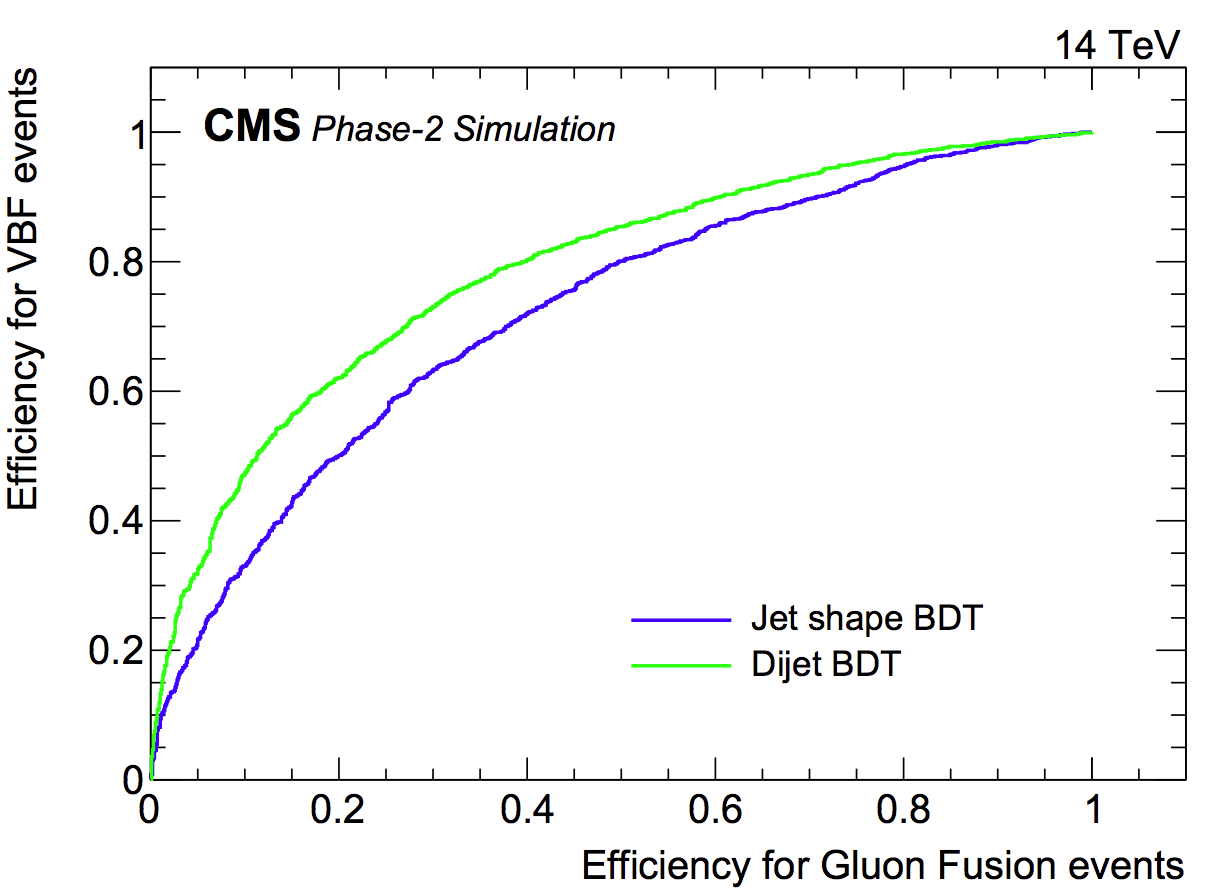
\includegraphics[width=0.8\textwidth]{Figures/HGCAL/VBFvsGGH.png}
  \caption[VBF and ggH selection efficiencies for two BDTs.]
  {
    The selection efficiency for VBF and ggH events for two different BDTs. 
    Figure taken from Ref.~\cite{HGCAL}.
  }
  \label{fig:hgcal_VBFvsGGH}
\end{figure}

Separately, another BDT is trained to reduce the amount of background entering analysis categories.
The VBF events are treated as signal, trained against prompt-prompt, 
prompt-fake and fake-fake \Hgg backgrounds.
This classifier uses only the kinematics of the the two photons as inputs. 
It is less powerful than the Run~2 equivalent 
because not all of the inputs used in the Run~2 version are available.
These include the photon identification score, 
the mass resolution estimates, and the vertex probability estimate.

A 2D scan was used to choose cut values on both the dijet and background BDTs, 
and generate the working points in Table \ref{tab:hgcal_yields}.
The working points were chosen to maximise the total expected significance, 
using the simple metric of the sum in quadrature of the 
the ratio of signal events to the square root of signal plus background events
for each working point~\cite{Asymptotic}.
The number of signal events selected, the fraction of ggH and VBF events, 
and the background per GeV are shown.
Also included is a Run~2 working point, 
consisting of all the events entering the analysis' three VBF tags, for comparison.

%TODO check these numbers
\begin{table}
  \centering
  \begin{tabular}{ r | c |  c |  c |  c }
  \multirow{2}{*}{Event Categories} &\multicolumn{3}{c|}{SM 125 GeV Higgs boson expected signal} & Bkg \\
    &  Total & ggH & VBF & per GeV \\
  \hline
  WP 0 &            750   &  25.4 \%  &  74.6 \%  &  678  \\
  WP 1 &            1275  &  35.9 \%  &  64.1 \%  &  876  \\
  WP 2 &            1926  &  45.8 \%  &  53.2 \%  &  1353 \\
  Summed WP &       3951  &  38.7 \%  &  61.3 \%  &  2907 \\
  Run 2 summed WP & 3878  &  42.0 \%  &  58.0 \%  &  1984 \\
  \end{tabular}
  \caption{The signal and background yields for three working points, and the sum thereof.
  The dijet BDT cut is varied, with a fixed cut on the background BDT.
  Number of events given is for \SI{3000}{\fbinv} of collected data. 
  The Run~2 WP contains the sum of selected events in all three VBF categories, extrapolated to \SI{3000}{\fbinv}.
  Table taken from Ref.~\cite{HGCAL}.}
  \label{tab:hgcal_yields}
\end{table}

These results show that performance comparable to that in Run~2 
is achieved despite the increase in pileup.
The background numbers are slightly higher than in Run~2, 
but it is expected that this could be reduced by a classifier using further photon quality variables.

\section{Beam tests}

To validate the design of the HGCAL and ensure its behaviour is well-modelled by simulation, 
beam tests have been conducted at both CERN and Fermilab in 2016 and 2017. 
Prototype silicon modules representative of those in both the CE-E and CE-H were built, 
with plastic scintillator tiles modified from an existing detector 
developed by the CALICE collaboration~\cite{CALICE}.
At Fermilab, the available electron beams were of relatively low energy (up to \SI{32}{GeV}), 
and so a test configuration with thickness of around $\SI{15}{X_0}$ was used.
A set of sixteen silicon modules, arranged in sixteen layers, were used.
At CERN, energies of up to \SI{250}{GeV} were available but with only eight modules.
The chosen setup therefore comprised eight layers placed between 5 and $\SI{27}{X_0}$.

Comparisons to simulation of the measured electron energy resolution 
and shower shape are shown in Figure~\ref{fig:hgcal_BeamTest}.
The variable E1/E7 is defined as the ratio of the energy in the most energetic cell (E1) 
to the sum of the energies of the most energetic cell and its six surrounding cells (E7);
this indicates the lateral extent of the shower.
Also shown is the relative energy resolution for a range of energy values, 
using both the CERN and Fermilab setups.
In both cases, excellent agreement is observed between data and simulation;
observed distributions match those predicted by simulation to within 5\%. 
These beam test results are particularly important because 
they constitute the first demonstration that the HGCAL behaves as predicted by simulation.

Furthermore, additional tests confirm the expected intrinsic timing capabilities of the silicon sensors, 
with the timing resolution measured to be less than \SI{30}{\pico\second}.
The timing performance of the silicon was also measured to be a function of S/N only, 
meaning it does not degrade with increasing radiation exposure. 

\begin{figure}[h!]
  \centering
  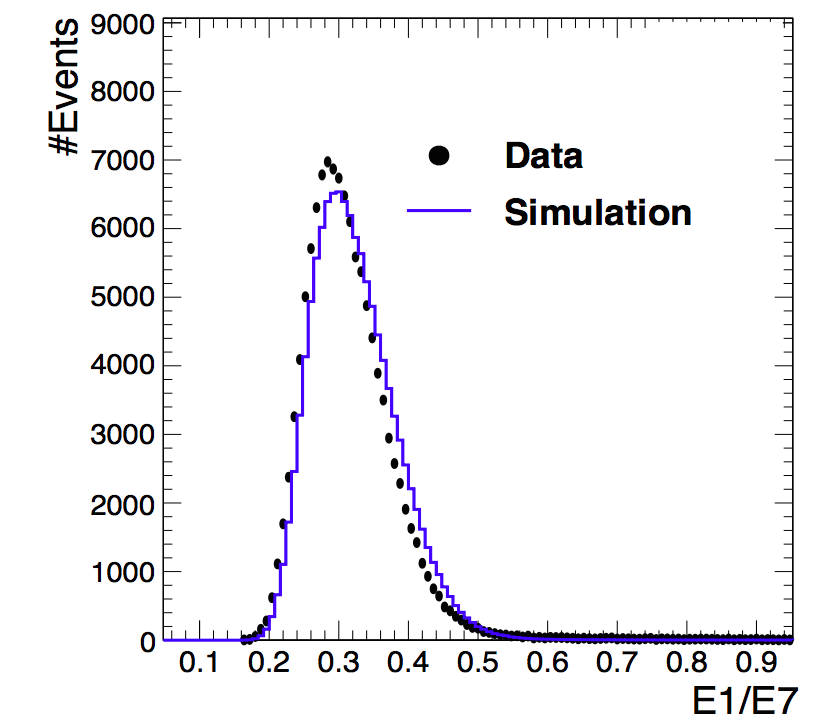
\includegraphics[width=0.49\textwidth]{Figures/HGCAL/BeamTestShape.png}
  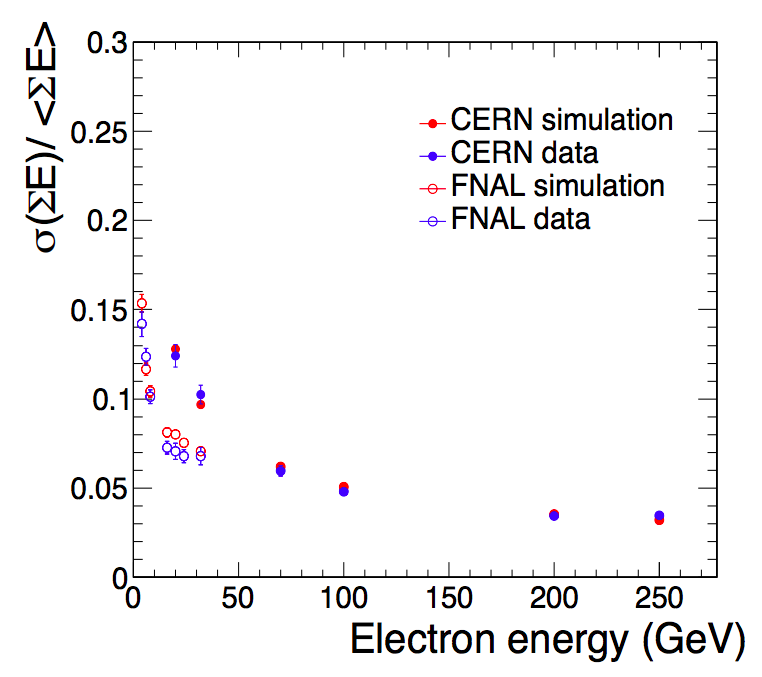
\includegraphics[width=0.49\textwidth]{Figures/HGCAL/BeamTestEnergy.png}
  \caption[Comparison of data and simulation in HGCAL beam tests.]
  {
    Left: the distribution of the energy ratio E1/E7 (defined in the text) for \SI{100}{GeV} electrons
    using the CERN beam test setup.
    Data points are shown in black and the blue histogram represents the simulation.
    Right: the relative electron energy resolution as a function of energy, 
    for both the CERN (solid circles) and Fermilab (hollow cirlces) setups.
    Simulated points are shown in red, with data points in blue.
    Figures taken from Ref.~\cite{HGCAL}.
  }
  \label{fig:hgcal_BeamTest}
\end{figure}

\chapter{Event Reconstruction and Selection}
\label{chap:objects}

\section{Introduction}

Measurements of Higgs boson properties can be made 
by directly using the diphoton invariant mass distribution.
Photon pairs resulting from Higgs boson decays produce a narrow signal peak, 
centred at the value of the Higgs boson mass, 
on top of the smoothly falling background distribution produced by other SM processes.
The Higgs boson mass is inferred from the two photons by constructing the diphoton invariant mass, 
which is given by the following expression
\begin{equation}
\label{eq:obj_mgg}
\mgg = \sqrt{ 2 E_{\gamma_1} E_{\gamma_2} (1 - \cos{\theta}) } ,
\end{equation}
where $E_{\gamma_1}$ and $E_{\gamma_2}$ is the energy of each photon, 
and $\theta$ is the opening angle between them.
The sensitivity of the analysis is maximised 
when the reconstucted diphoton mass peak is as narrow as possible, 
thereby minimising the diphoton mass resolution.
This requires the two photons to be correctly identified 
and their positions and energies accurately measured.
Furthermore, the location of the interaction vertex from which the photons originated 
must be established in order to calculate the opening angle.
Additional objects in the event, including jets and leptons, 
are further used to improve the sensitivity of the analysis 
and measure different Higgs boson production processes.

This section describes the official CMS procedure for reconstructing physics objects using the particle flow algorithm \cite{ParticleFlow}.
In addition, the photon and vertex identification techniques specific to the \Hgg analysis are detailed.
The approach used is almost identical between the 2016 and 2017 datasets; 
any differences are highlighted in the text.

\section{Particle flow}
The global event description at CMS is formed using the particle flow (PF) algorithm~\cite{ParticleFlow}.
The goal of PF is to optimally combine the information of all the CMS subdetectors, 
enabling the best possible identification and energy measurements for all types of objects.
Inputs to the PF algorithm are tracks originating from the tracker and muon system, 
and calorimeter clusters from the ECAL and HCAL.
CMS is able to benefit from the PF approach due to its strong magnetic field, 
alongside the fine segmentation and hermeticity of the tracker, calorimeters, and muon system.
Together these allow different types of objects to be separately identified, 
and the energy measurement to be driven by the subdetector with the best resolution.

Tracks are reconstructed from hits in the tracker using multiple iterations of a combinatorial track-finding procedure \cite{TrackReco}.
Each iteration proceeds in the following way.
First, track seeds comprising two or three hits are chosen, defining the initial track parameters.
Then an extrapolation is performed along the expected track paths, adding any additional hits consistent with the path hypothesis.
Next the track parameters are re-estimated, and the track candidate collection is pruned based on quality criteria.
All the selected hits are then removed from consideration in the following iterations.
In this way, the first iteration identifies the most obvious tracks, normally those with high \pt and near to the interaction point.
The complexity of the subsequent iteration is reduced since many hits have been removed.
This therefore permits lower thresholds to be used and tracks with lower \pt or highly displaced tracks to be found.
In addition, an independent procedure is used to construct muon tracks from hits in the muon system.

In the calorimeters, a clustering algorithm is used to collect together energy deposits belonging to each shower. %no clustering in HF
The procedure in the ECAL is described here, since it is an important input to the \Hgg analysis; the HCAL procedure is similar.
The clustering algorithm begins by selecting cluster seeds, which have an energy above a threshold and higher than any neighbouring crystal \cite{PhotonReco}.
So-called topological clusters are then constructed iteratively by adding deposits which share a side or corner with one already in the cluster, 
provided their energy exceeds a threshold dependent on the noise level. %extra E_T requirement in the endcaps. 
%Threshold is 2sigma noisce, ~80 MeV in barrel and up to 300 MeV in endcaps
If a crystal could be included in more than one topological cluster, its energy is shared between them assuming a Gaussian shower shape.
Finally, topological clusters are grouped into so-called superclusters (SCs).
This step is designed to recover energy lost via bremsstrahlung; 
radiated showers typically have very similar $\eta$ values 
but are spread out in the $\phi$ direction by the magnetic field.

Given these tracks and calorimeter clusters as inputs, the particle flow algorithm forms collections of candidates for five types of particle:
\begin{itemize}
  \item{\textbf{Muons:} a path extrapolated from the tracker is consistent with a muon track. 
                        The energy is inferred from the curvature of the track.}  %actually uses muon info too when pT > 200 GeV - check details
  \item{\textbf{Electrons:} an ECAL SC is present and associated with a track from the inner tracker. 
                            The energy is measured using a combination of the track \pt and the SC energy.}
  \item{\textbf{Photons:} an ECAL SC is present and no track is associated with it.
                          The energy is measured using the ECAL SC only.}
  \item{\textbf{Neutral hadrons:} matched ECAL and HCAL clusters with no associated track.
                                 Energy measurement is the sum of the cluster energies.}
  \item{\textbf{Charged hadrons:} a track is matched to ECAL and HCAL clusters.
                                 The track curvature is used together with the calorimeter deposits to calculate the energy.}
\end{itemize}
In this way, the central CMS software provides analyses with physics objects 
ready for use in measurements.
The remainder of this chapter describes how these objects are used in the \Hgg analysis.

\section{Samples}
\subsection{Data}

This analysis is based on a total of \SI{77.4}{\fbinv} of p-p collision data collected by CMS at $\sqrt{s}\,=\,\SI{13}{TeV}$.
Of this, \SI{35.9}{\fbinv} was collected during 2016 and \SI{41.5}{\fbinv} in 2017.

Data selected for use in the analysis must first be selected by the CMS trigger system, 
which reduces the total event rate to an acceptable level.
This two-step system requires each high-level trigger (HLT) path to be seeded by at least one electromagnetic candidate at the level one trigger (L1T).
A higher efficiency is obtained if only one of the two photons is required to be present at level one; 
however since this results in a high event rate, a stringent \pt selection is required.
The threshold is dependent on instantaneous luminosity and the photon isolation, 
but is typically set at \SI{40}{GeV}.
This results in loss of efficiency in \Hgg events, so asymmetric HLT paths seeded by two electromagnetic candidates are also used.
During 2016 data-taking, the \pt thresholds at L1 were 22 and \SI{15}{GeV} for the leading and subleading candidates.
In 2017, this was increased to 25 and \SI{14}{GeV} respectively. %TODO check this is bc of PU/int lumi only

At the HLT, a clustering procedure similar to that used offline is performed. 
This allows shower shape and photon isolation variables to be included in the selection criteria.
These include the ratio of energy in a $3\times3$ grid of crystals to that of the SC (\RNINE), 
and the ratio of energy in the HCAL behind the SC to the SC energy.
Together with asymmetric requirements on the photon \pt and a cut on the diphoton mass, 
these form the HLT selection.
In 2016, the HLT \pt thresholds were 30 and \SI{18}{GeV} respectively;
this increased to 30 and \SI{22}{GeV} in 2017.

The efficiency of the trigger selection is measured using the tag and probe technique in \Zee events where the electrons are reconstructed as photons.
In this method, dielectrons consistent with decays from the $Z$ boson are selected, 
and a tight identification requirement is placed on one electron (known as the tag).
The second electron (the probe) must then pass a very loose requirement, 
and the efficiency of the additional HLT selection criteria can be measured.
The trigger efficiency is over 97\% in the barrel and above 95\% in the endcaps.
In simulation, its effect is accounted for by applying weights binned in \pt, $\eta$ and \RNINE.

\subsection{Simulation}

Various types of events are simulated with Monte Carlo (MC) techniques for use in training event classifiers, 
producing the signal model, and for performing validation of the analysis.

The signal simulation used to produce the final signal model is generated using \textsc{MadGraph5_{}aMC@NLO} \cite{Madgraph}, 
which is next-to-leading order in perturbative QCD.
This is interfaced to \textsc{PYTHIA}~\cite{pythia} to perform the parton showering and hadronisation, 
using the tune \textsc{CUETP8M1}.
Events from ggH production are then reweighted to agree with the next-to-next-to-leading order program \textsc{NNLOPS}~\cite{NNLOPS}.
Additional independent signal samples are produced using \textsc{POWHEG}~\cite{powheg}. %these are used to optimise the analysis category definitions without bias.

Simulated background events are not used to produce the final results of the analysis, 
but are used to train several of the classifiers used in the analysis.
The predominant source of back is the irreducible SM production of two prompt (real) photons, 
which is simulated using the \textsc{SHERPA}~\cite{sherpa} program. %Born processes up to three jets and boxes at LO
There are two types of reducible background: $\gamma$ + jet events where the jet is misidentified as a photon (``prompt-fake" events), 
and events where two jets are misidentified as photons (``fake-fake" events).
These are both modelled using \textsc{PYTHIA}, 
with filters applied to increase the number of events containing jets with high electromagnetic energy fractions.
The Drell-Yan events used extensively in the analysis validation are simulated using \textsc{MadGraph5_{}aMC@NLO} \cite{Madgraph}. 

The CMS detector itself is modelled using \textsc{GEANT4} \cite{Geant4}.
This simulation includes additional pileup interactions.
The number of pileup events is corrected to agree with data, 
where an average of 23 and 32 pileup interactions were observed in 2016 and 2017 data-taking respectively.

\section{Photon reconstruction}
\subsection{Overview}

Photons to be used in the \Hgg analysis are selected from the PF set of photon candidates.
The energy of each photon candidate is estimated from the SC, 
which includes deposits from the many particles comprising the electromagnetic shower.
In some cases, photons will interact with detector material upstream of the ECAL 
and produce an electron-positron pair; these are known as ``converted" photons.
Converted photons will also deposit energy in the ECAL preshower detector, 
which is included in the SC energy estimate.
A correction is then made to this SC energy using a multivariate regression technique.
After that, data and MC are brought into agreement by applying additional scale and smearing corrections to the photon energies.
The details of the energy estimation procedure are described in Section~\ref{sec:objects_PhotonEnergy}.
Once the photon energy has been established, 
a set of preselection criteria is applied to obtain the final set of photons considered in the analysis.
One of these criteria is a requirement placed on the output score of the photon identification BDT, 
which is trained to reduce the contamination from other objects which mimic real photons.
The full set of preselection requirements, including the photon identifiaction BDT, 
are described in Sections~\ref{sec:objects_PhotonPresel} and \ref{sec:objects_PhotonIDBDT}.

\subsection{Variable definitions}

Different types of variables are used in the photon reconstruction.
They can be divided into shower shape and isolation variables.
The ECAL shower shape information is used both to correct the energy and discriminate between real and fake photons.
Isolation variables can be used to reduce the mis-identification of jets and other objects imitating a real photon signal.
The full set of variables used in this section and their definitions are given below.
\\ \\
\textbf{Shower shape variables:}
\begin{itemize}[noitemsep]
  \item \emph{$E_{2\times2}/E_{5\times5}$}: the ratio of the energy in the $2\times2$ grid
    containing the most energetic cells in the SC to the energy in
    the 5x5 grid centred on the SC seed.
  \item \emph{$\textrm{cov}_{i\eta i\phi}$}: the covariance of the single crystal $\eta$
    and $\phi$ values in within the 5x5 grid centred on the
    SC seed.
  \item \emph{$\sigma_{i\eta i\eta}$}: the standard deviation of the 
    shower in terms of number of crystal cells. 
  \item \emph{$\RNINE$}: $E_{3\times3}/\Eraw$ where $E_{3\times3}$ is the energy sum of the
    $3\times3$ grid surrounding the SC seed and $\Eraw$ is the energy sum of the SC before corrections. 
  \item \emph{$\sigma_{\eta}$}: the standard deviation
    of single crystal $\eta$ values within the SC, weighted by the logarithm of the crystal energy.
  \item \emph{$\sigma_{\phi}$}: the standard deviation
    of single crystal $\phi$ values within the SC, weighted by the logarithm of the crystal energy.
  \item \emph{$\sigma_{RR}$}: the standard deviation of the shower
    spread in the x-y plane of the preshower detector (endcap only).
\end{itemize}

\textbf{Isolation variables:}
\begin{itemize}[noitemsep]
  \item $H/\Eraw$: the ratio of the energy in the HCAL cells behind the SC 
    and the SC energy.
  \item \emph{$\mathcal{I}_{\text{ph}}$}: 
    photon isolation,
    defined as the sum of the transverse energy of the particles
    identified as photons falling inside a cone of radius
    $R=0.3$
    around the photon candidate.
  \item \emph{$\mathcal{I}_{\text{tk}}$}: 
    track isolation, which is 
    the sum of the transverse momenta
    of all tracks in a cone of radius $R=0.3$
    around the photon candidate (with tracks in an
    inner cone of size $R=0.04$ not included in the sum).
    %the cone is hollow because the isolation definition is 
    %also used for electrons, and the track from the electron
    %itself is excluded;
  \item \emph{$\mathcal{I}_{\text{ch}}$}: 
    charged hadron isolation,
    the sum of the transverse momenta of
    charged particles inside a cone of radius $R<0.3$ around the
    photon candidate.
\end{itemize}

\textbf{Miscellaneous:}
\begin{itemize}[noitemsep]
  \item \emph{Electron veto}: rejects the photon candidate if its 
    supercluster is matched to an electron track.
  \item \emph{$\rho$}: the median energy  density per unit area in the event.
  \item \emph{\Eraw}: the energy of the supercluster before corrections.
  \item \emph{\Etrue}: the true photon energy.
\end{itemize}

\subsection{Photon energy}
\label{sec:objects_PhotonEnergy}

The photon supercluster energy is computed from the calibrated ECAL SC, as described in Section~\ref{sec:detector_ECAL}.
However, this energy estimate is imperfect for several reasons.
Firstly, the SC may not capture all the energy of an electromagnetic shower and therefore underestimate the photon energy.
This can occur when the photon interacts with material before the ECAL and therefore begins to shower before reaching the ECAL, 
resulting in both energy lost in the material and a dispersed shower which is not contained by the SC.
In addition, leakage can occur into the gaps between crystals and modules in the ECAL, 
as well as through the back of the ECAL if the showering begins near the end of a crystal.

The energy estimate provided by the uncorrected SC (\Eraw) can therefore be significantly improved by the use of a multivariate regression.
This provides an additional energy correction to each reconstructed photon, so that the photon energy in simulation agrees with the true photon energy.
The training objective for the regressor is to learn the parameters of the $\Etrue/\Eraw$ probability distribution function, 
which is parameterised as a Gaussian core with power law tails on each side. %i.e. DCB + 1G
There are a large number of inputs to the regressor which account for different effects.
These include information relating to the shower shape, the position of the SC, the seed crystal, and the energy density in the event.

The shower shape and position variables enable the difference in shower containment due to variations in the ECAL geometry, 
and the showering induced by upstream material, to be corrected.
Variables relating to the seed crystal position within the SC and energy ratios formed using the seed account for the local shower containment.
The energy density and number of vertices accounts for any additional energy included due to pileup.

The most probable value of the pdf returned by the regression is used to correct the supercluster energy for each photon.
The distribution is also used to infer the per-photon uncertainty on the energy.
This resolution estimate is then used in the classification of events, as described in Chapter~\ref{chap:categorisation}.

After the regression, additional corrections are applied to account for differences between data and simulation.
The first of these is to correct the energy scale in data;
the detector response changes to damage from radiation during LHC operation and subsequent recovery during LHC down time.
This can cause the measured energy to both drift slowly and change discontinuously over time.
Corrections are derived using \Zee events where the electrons are reconstructed as photons, using the known $Z$ boson mass.
These corrections are extracted differentially in time, and binned in the photon $\eta$ (two bins in each of barrel and endcap) and \RNINE (two bins).
Their magnitude varies from 0.1-0.3\% in the barrel and from 0.2 to 2\% in the endcaps.

Finally, the energy resolution in simulation is corrected to match that in data.
This is implemented as a Gaussian smearing using the same bins as the energy corrections.
The size of the corrections range from approximately 0.1 to 2.7\%.
Once all the corrections have been applied, the photon energy resolution ranges from around 1 to 2.5\% in the barrel
and from 2.5\% to 3.5\% in the endcaps.
Validation of the energy after corrections is shown in Figure~\ref{fig:obj_mee}, 
where data is compared to simulation in \Zee events with electrons reconstructed as photons.
Full details of the entire energy correction procedure can be found in Ref.\cite{PhotonReco}.

\begin{figure}[h!]
  \centering
  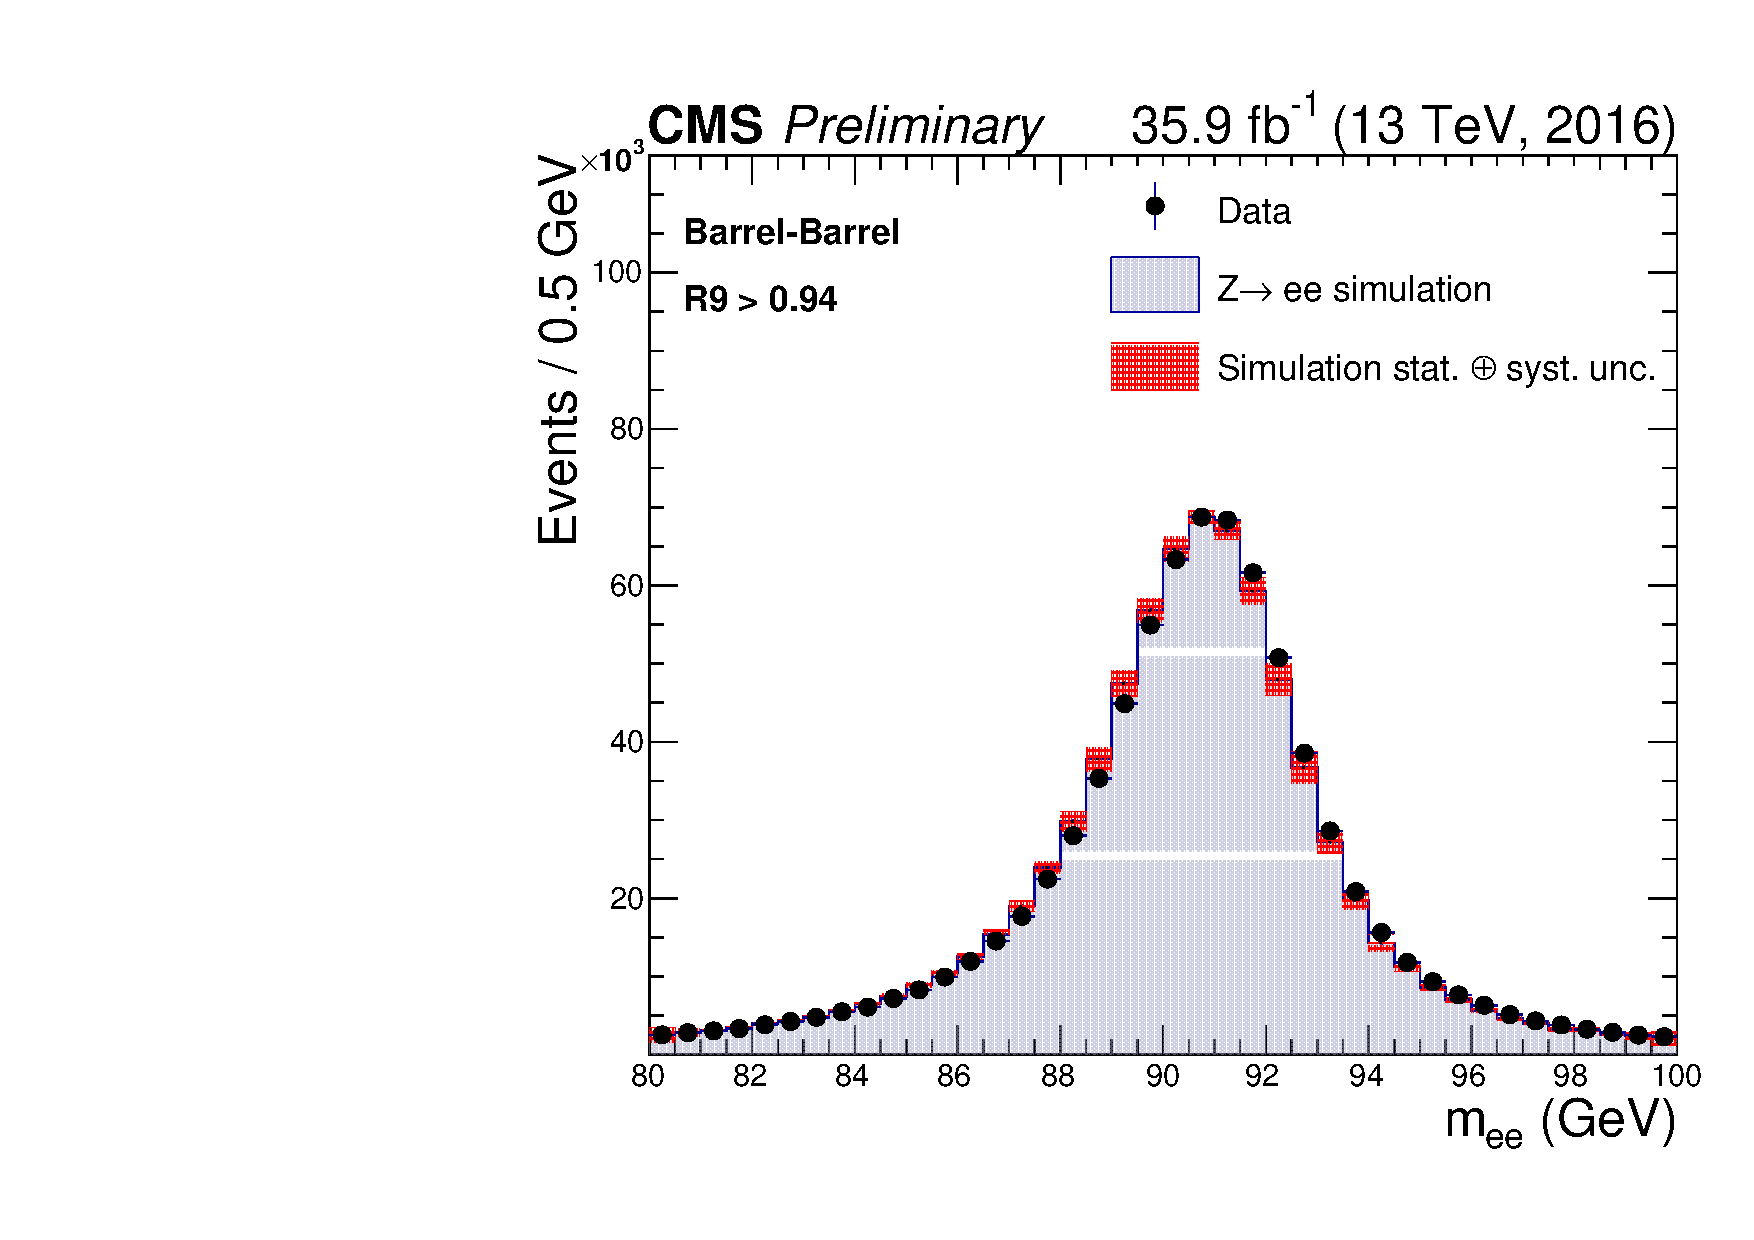
\includegraphics[width=0.49\textwidth]{Figures/Objects/meeBarrel2016}
  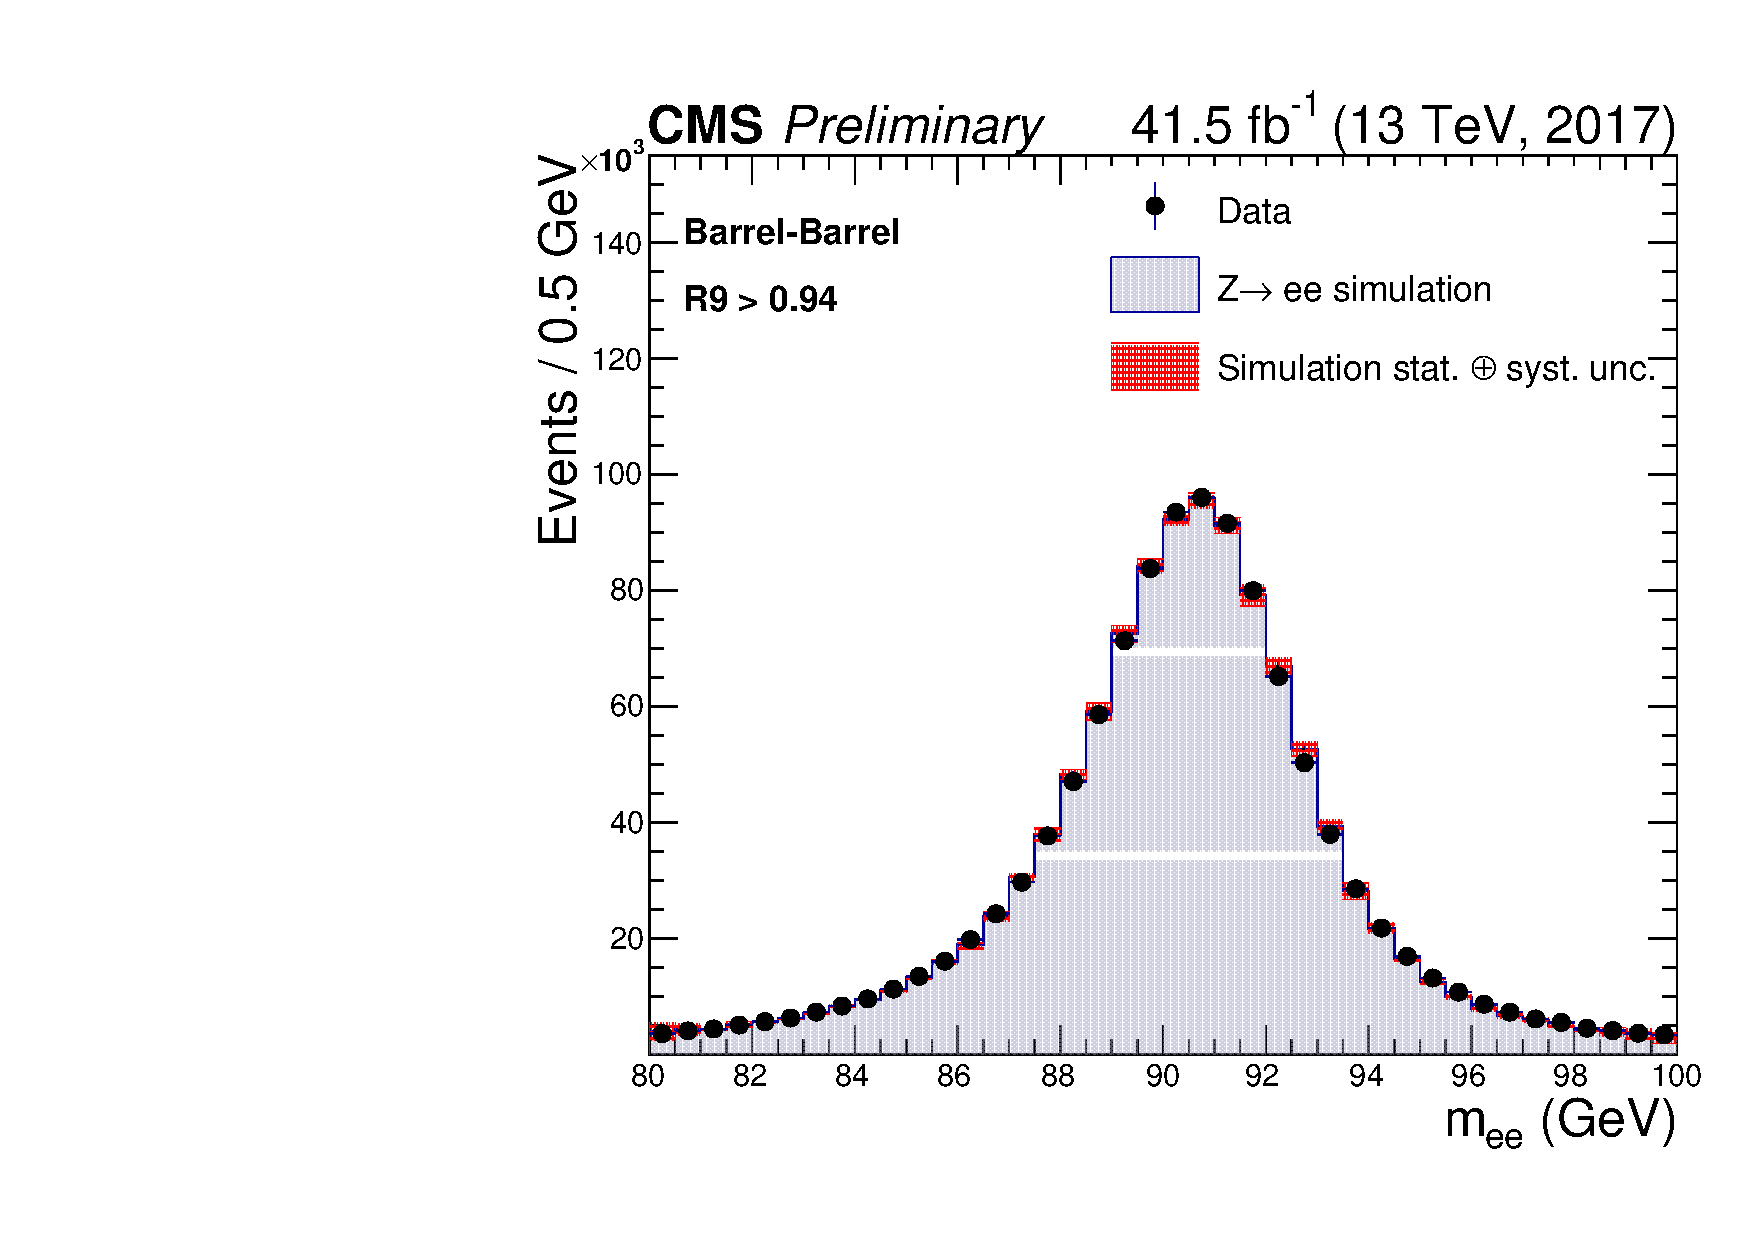
\includegraphics[width=0.49\textwidth]{Figures/Objects/meeBarrel2017} \\
  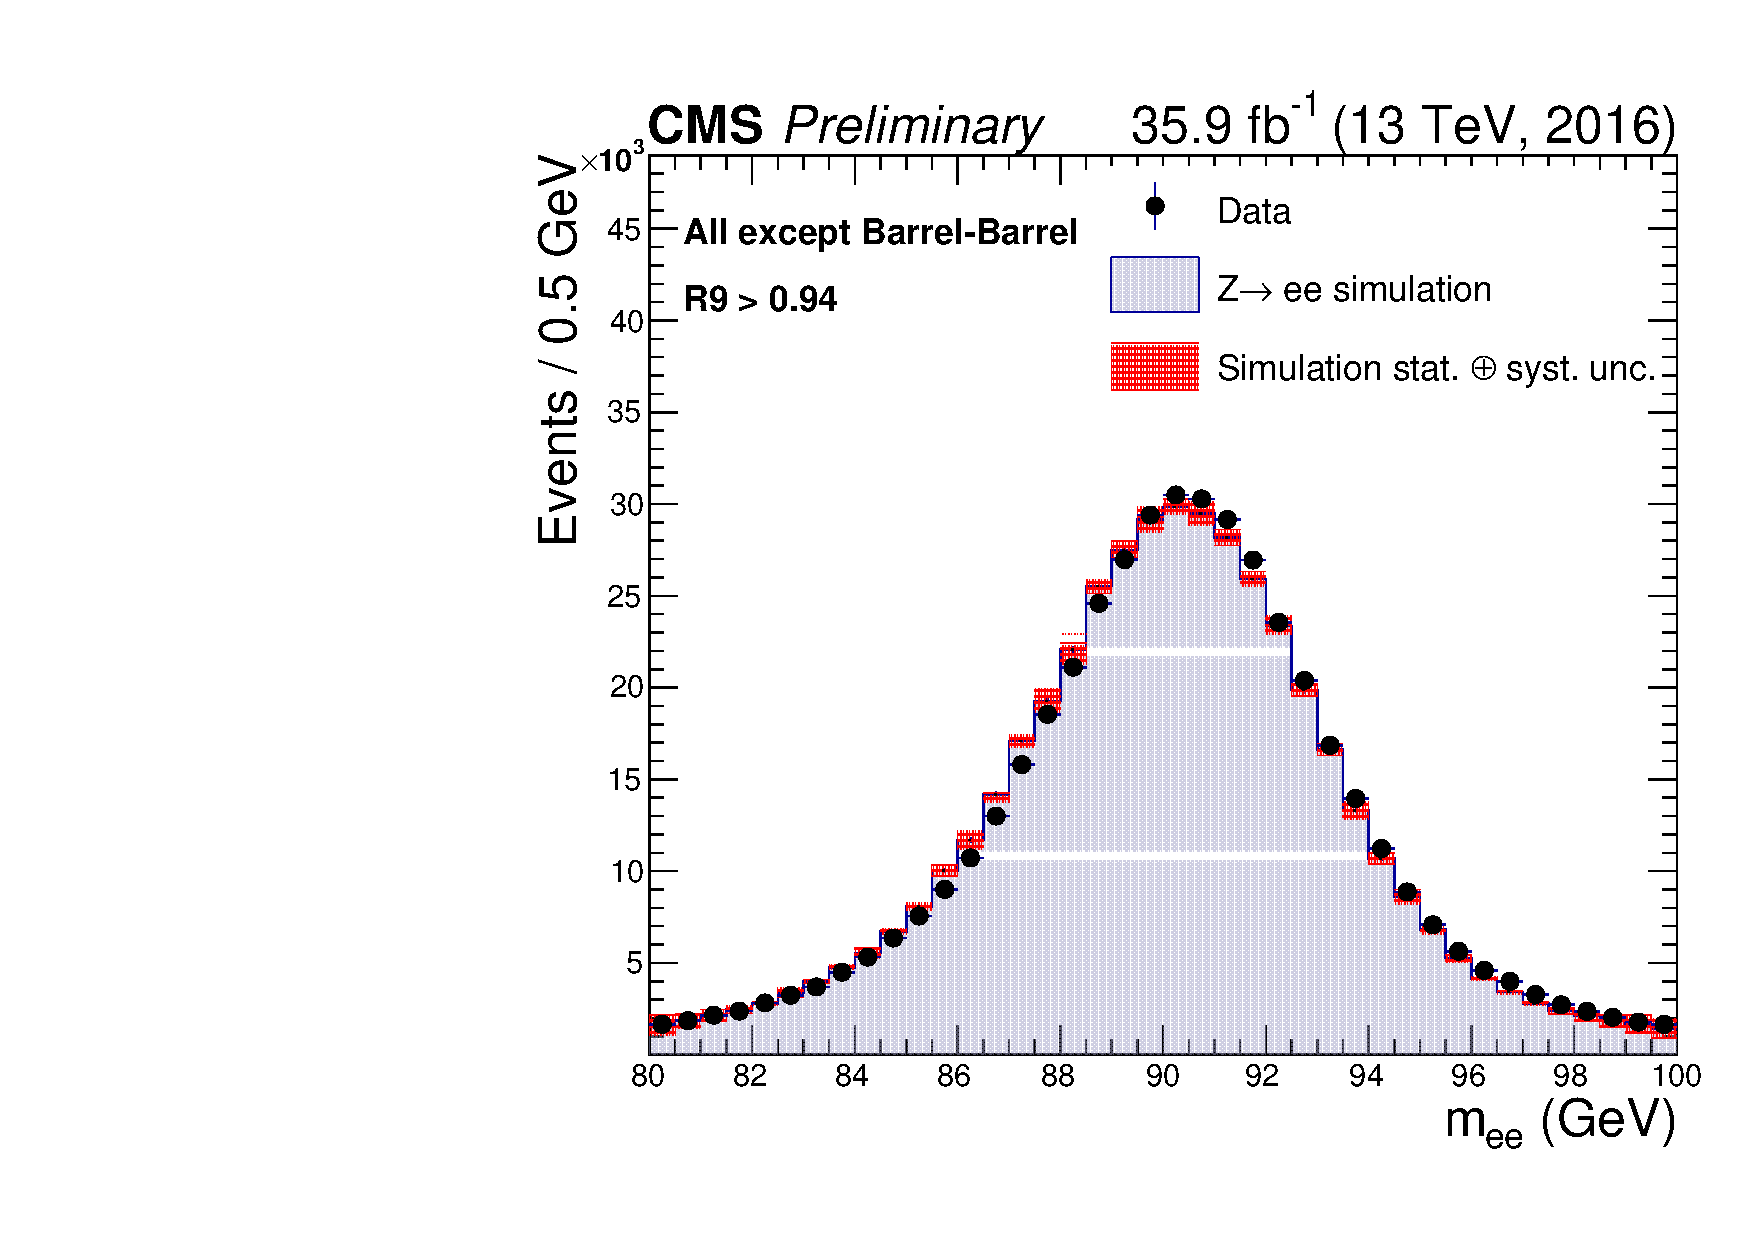
\includegraphics[width=0.49\textwidth]{Figures/Objects/meeEndcap2016}
  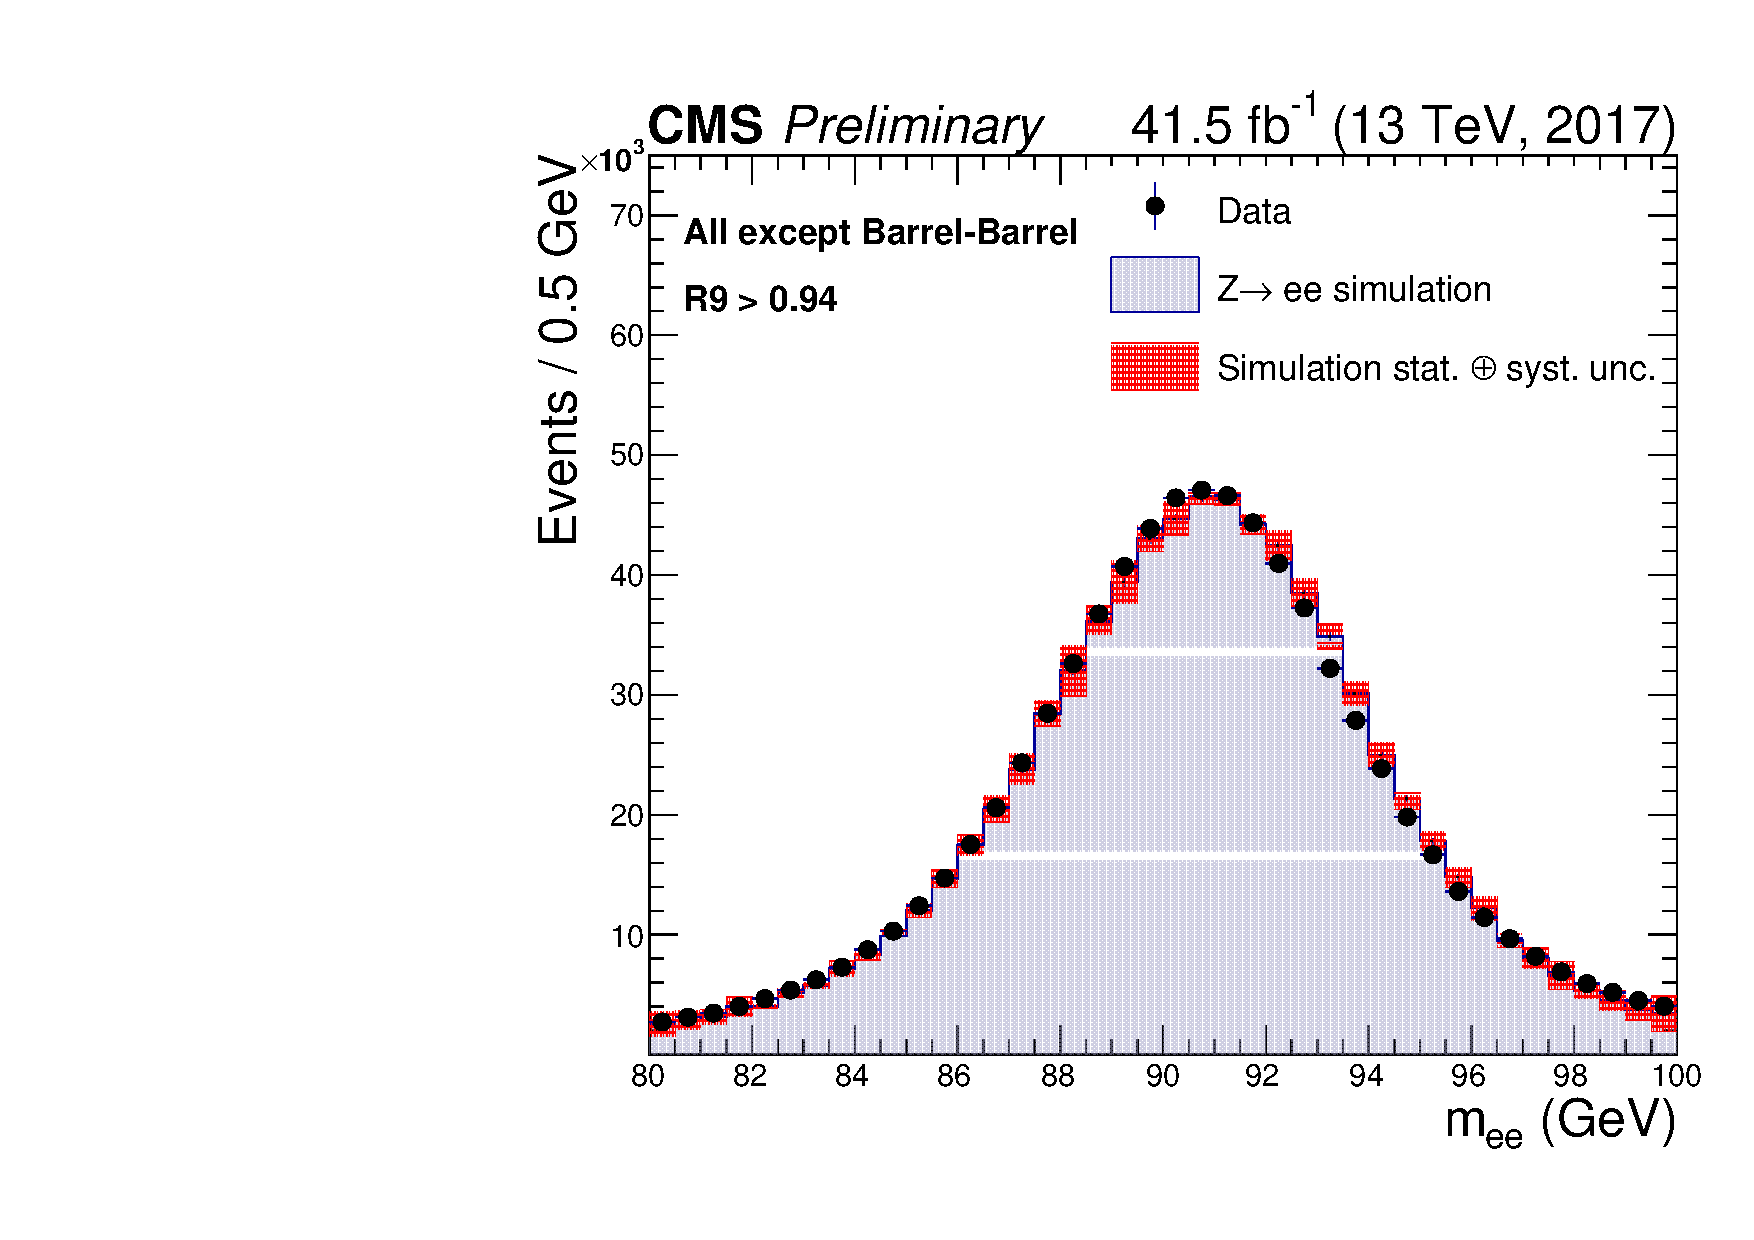
\includegraphics[width=0.49\textwidth]{Figures/Objects/meeEndcap2017}
  \caption[Dielectron invariant mass distributions.]
  {
    Comparison of the dielectron invariant mass distributions in data and simulation
    (after energy smearing) for \Zee
    events where electrons are reconstructed as photons.
    The \RNINE variable is required to be greater than 0.94.
    The simulated distributions are
    normalised to the integral of the data distribution 
    in the range $87 < m_{ee} < 93$ GeV to highlight
    the agreement in the bulk of the distributions.
    The comparison is shown for events where at both electrons are in the ECAL barrel (top), 
    and least one electron is not in the ECAL barrel (bottom).
    The plots on the left show data and simulation from 2016, 
    with 2017 data and simulation shown in the plots on the right.
  }
  \label{fig:obj_mee}
\end{figure}

\subsection{Photon preselection}
\label{sec:objects_PhotonPresel}

To be further considered in the \Hgg analysis, 
photons must pass a set of criteria designed to reduce the contamination from objects faking photons.
This preselection is similar to, but more stringent than, that required at trigger level.
The full set of requirements is:
\begin{itemize}[noitemsep]
  \item to be within the ECAL acceptance; this means $|\eta|\,<\,2.5$ and excluding the endcap transition region $1.44\,<\,|\eta|\,<\,1.57$.
  \item passing the electron veto
  \item $\pt > 30 (20)$ GeV for the leading (subleading) photon in 2016. 
  The thresholds are 35 and 25 GeV respectively in 2017, due to the tighter trigger requirements.
  \item either $\mathcal{I}_{\text{ch}} < 20$ GeV, 
  or $\mathcal{I}_{\text{ch}} / \pt < 0.3$ for photons with $\RNINE < 0.8$.
  \item an additional set of \RNINE and $\eta$-dependant shower shape and isolation requirements, 
  summarised in Table~\ref{tab:obj_preselection}.
\end{itemize}

\begin{table}[htbp]
  \begin{center}
    \begin{tabular}{l|c|c|c|c|c}
      \hline
      \multicolumn{1}{c|}{} & \RNINE & H/E     & $\sigma_{\eta \eta}$ & $\mathcal{I}_{\text{ph}}$ & $\mathcal{I}_{\text{tk}}$ \\
      \hline
      \multirow{2}{*}{Barrel}
      & $[0.5, 0.85]$  & $<0.08$ & $<0.015$ & $<4.0$ & $<6.0$
      \\
      & $> 0.85$   & $<0.08$ & --       & -- & --
      \\ \hline
      \multirow{2}{*}{Endcaps}
      & $[0.8, 0.90]$  & $<0.08$ & $<0.035$ & $<4.0$ & $<6.0$
      \\
      & $> 0.90$     & $<0.08$ & --       & -- & --
      \\ \hline
    \end{tabular}
  \end{center}
  \caption{Summary of photon preselection requirements.}
  \label{tab:obj_preselection}
\end{table}

The efficiency of these preselection criteria, aside from the electron veto, is measured using \Zee events.
To measure the electron veto efficiency, \Zmumug events are used.
Efficiencies range from over 94\% for high \RNINE photons in the barrel, 
to around 50\% for low \RNINE photons in the endcaps.
Very good agreement is observed between data and simulation. %0.1-0.3\% in barrel, 0.5-1\% in endcap

\subsection{Photon identification}
\label{sec:objects_PhotonIDBDT}

An additional part of the photon preselection is the photon identification BDT.
Its purpose is to discriminate between real photons and photon candidates passing the preselection which originate from other objects, 
such as jet fragments.
The BDT is trained using $\gamma$ + jet events passing the preselection described above, with real photons treated as signal and fake photons as background.
The inputs are similar to the those used in the energy regression, 
including shower shape and isolation variables.
In addition, pileup-sensitive variables $\rho$ and the number of interaction vertices, 
together with photon kinematic varialbes, are used as inputs.

A loose selection on the photon identification BDT at -0.9 completes the analysis preselection.
The output score on preselected diphoton events is shown in Figure~\ref{fig:obj_IDMVA}.
Additional validation using \Zee events is demonstrated in Figures~\ref{fig:obj_ZeeIDMVA}.

\begin{figure}[h!]
  \centering
  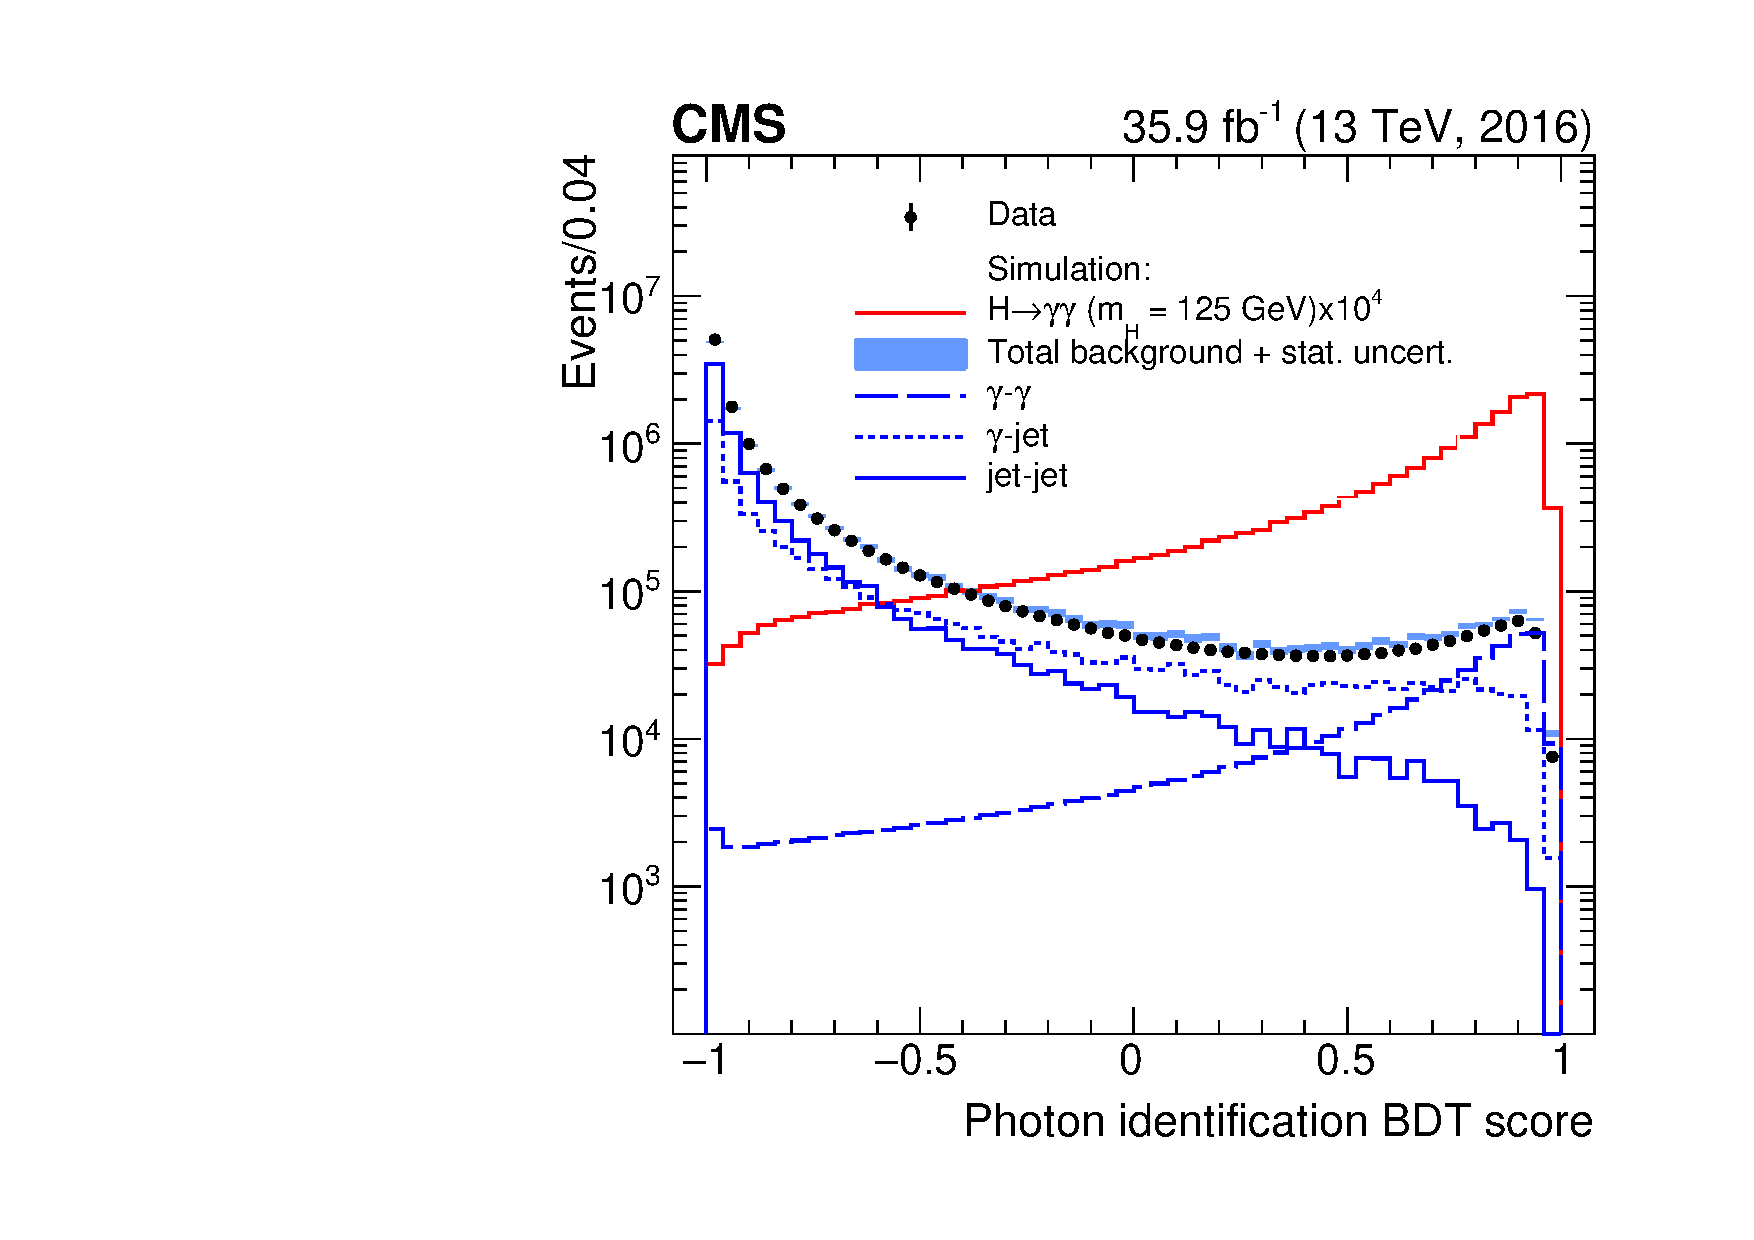
\includegraphics[width=0.49\textwidth]{Figures/Objects/IDMVA2016}
  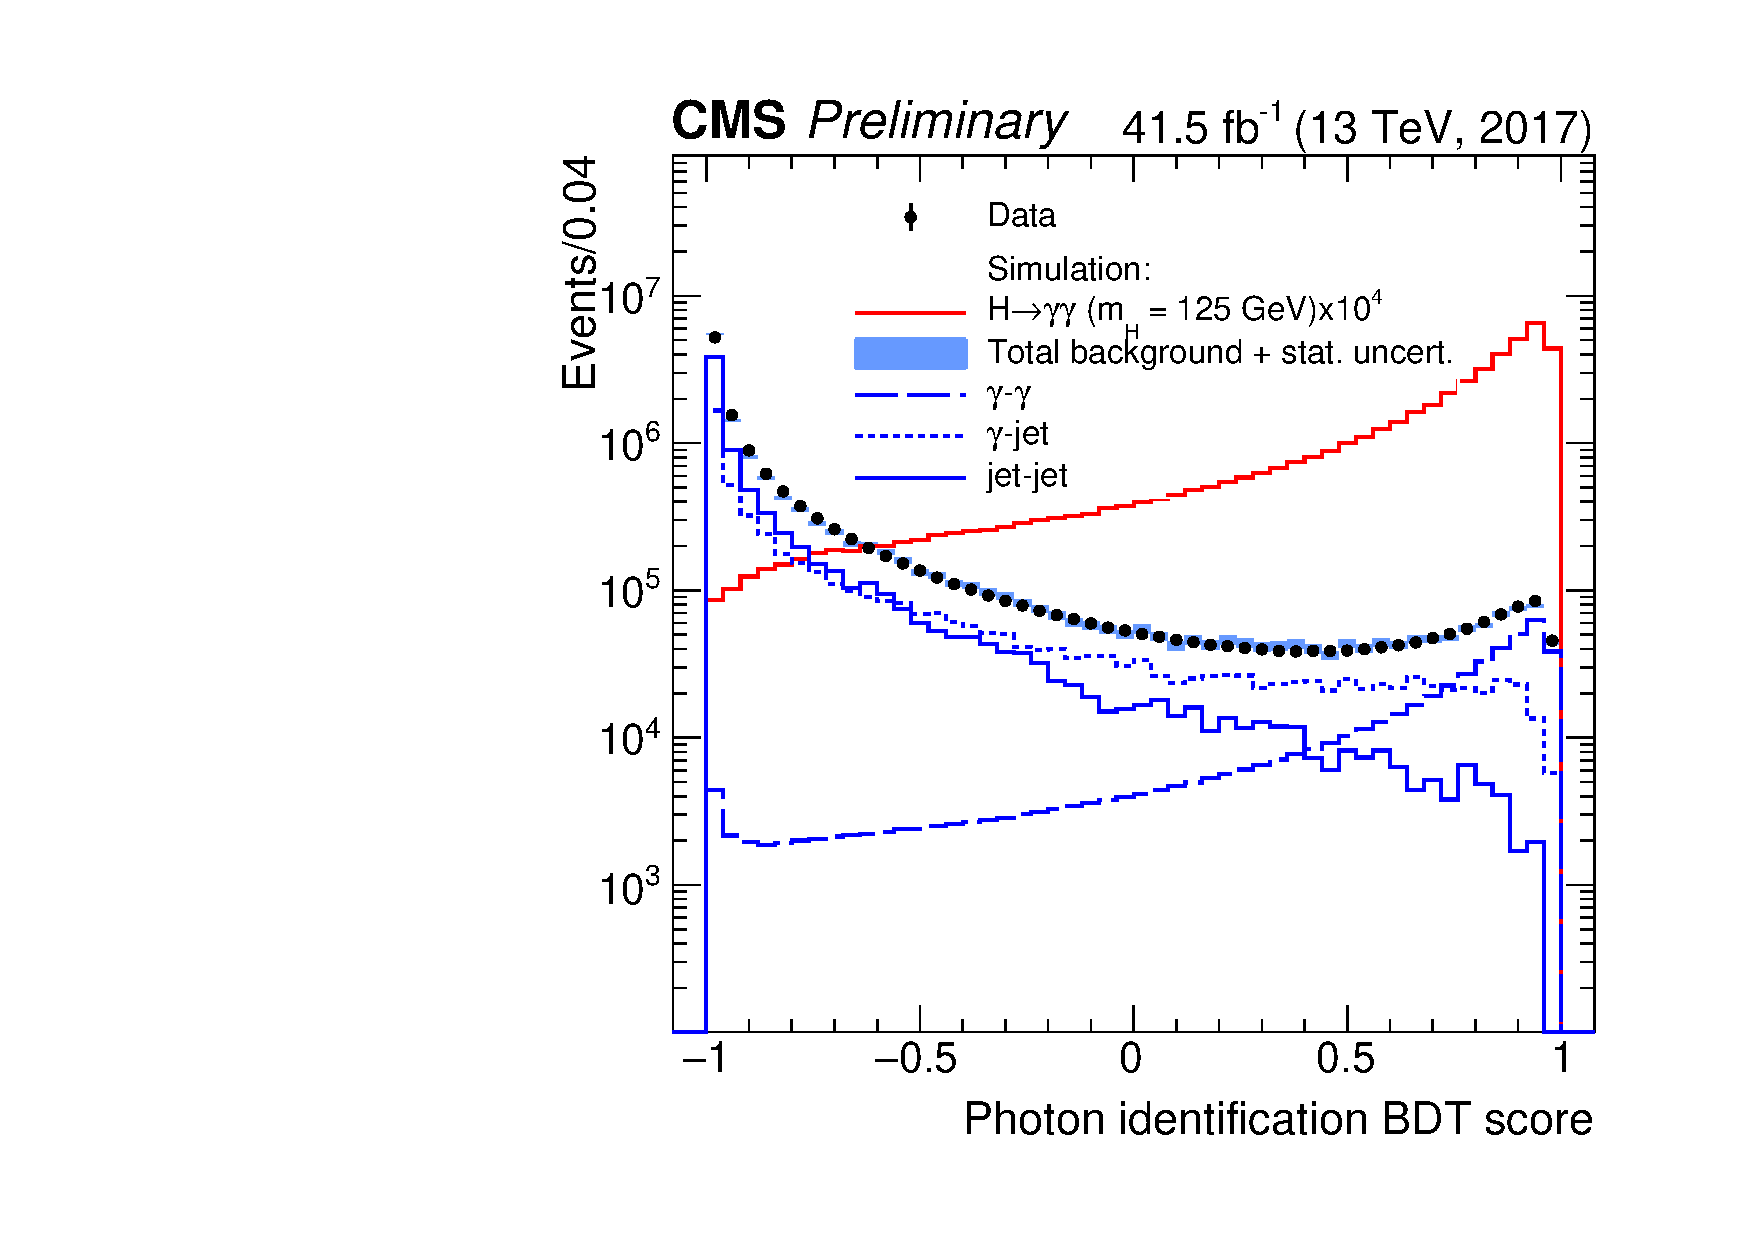
\includegraphics[width=0.49\textwidth]{Figures/Objects/IDMVA2017}
  \caption[Photon identification BDT score distributions.]
  {
    Distribution of the photon identification BDT score of the lowest scoring photon
    of diphoton pairs with an invariant mass in the range $100 < \mgg < \SI{180}{GeV}$, 
    for events passing the preselection in data (black points), 
    and for simulated background events (blue histogram). 
    Histograms are also shown for different components of the simulated background.
    The sum of all background distributions is scaled up to data. 
    The red histogram corresponds to simulated Higgs boson signal events. 
    The left figure shows 2016 data and simulation, with 2017 data and simulation shown on the right.
  }
  \label{fig:obj_IDMVA}
\end{figure}

\begin{figure}[h!]
  \centering
  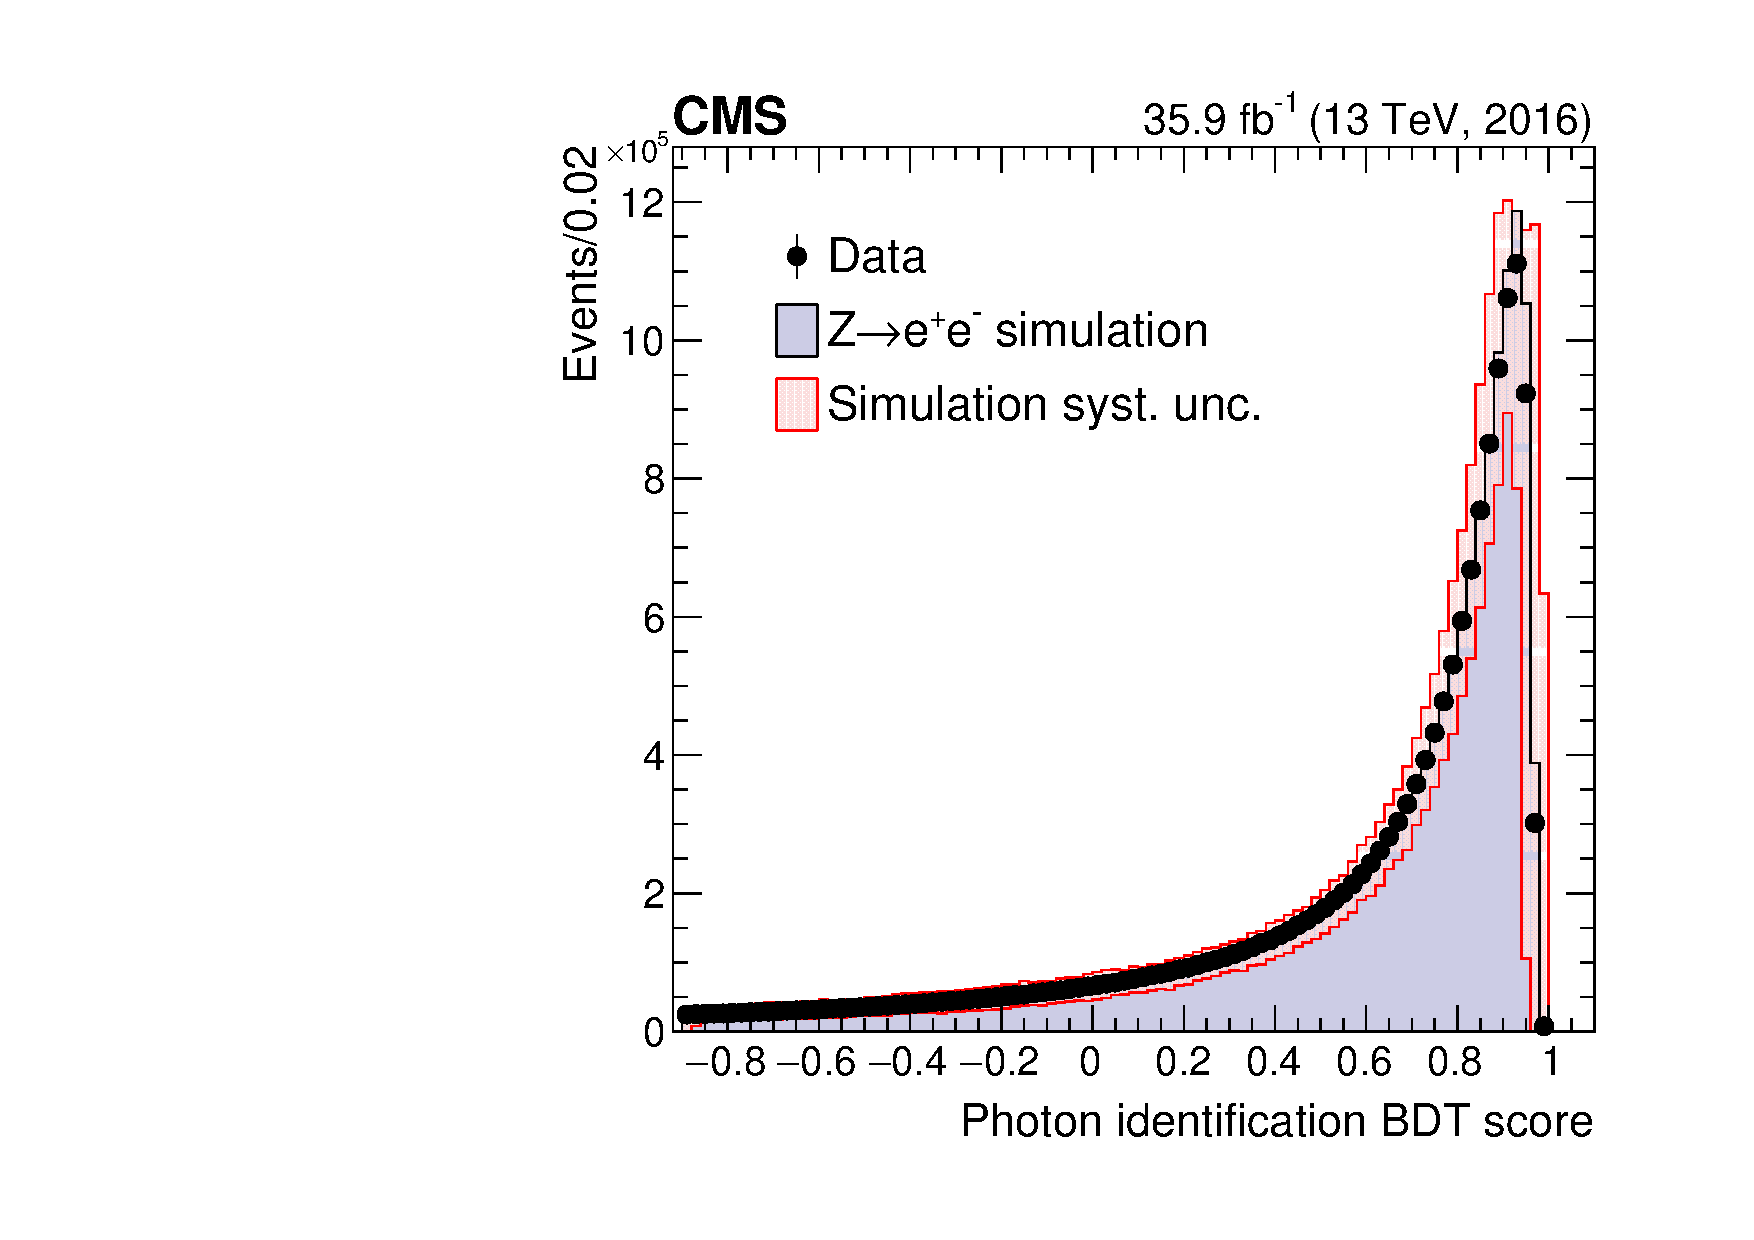
\includegraphics[width=0.49\textwidth]{Figures/Objects/ZeeIDMVA2016}
  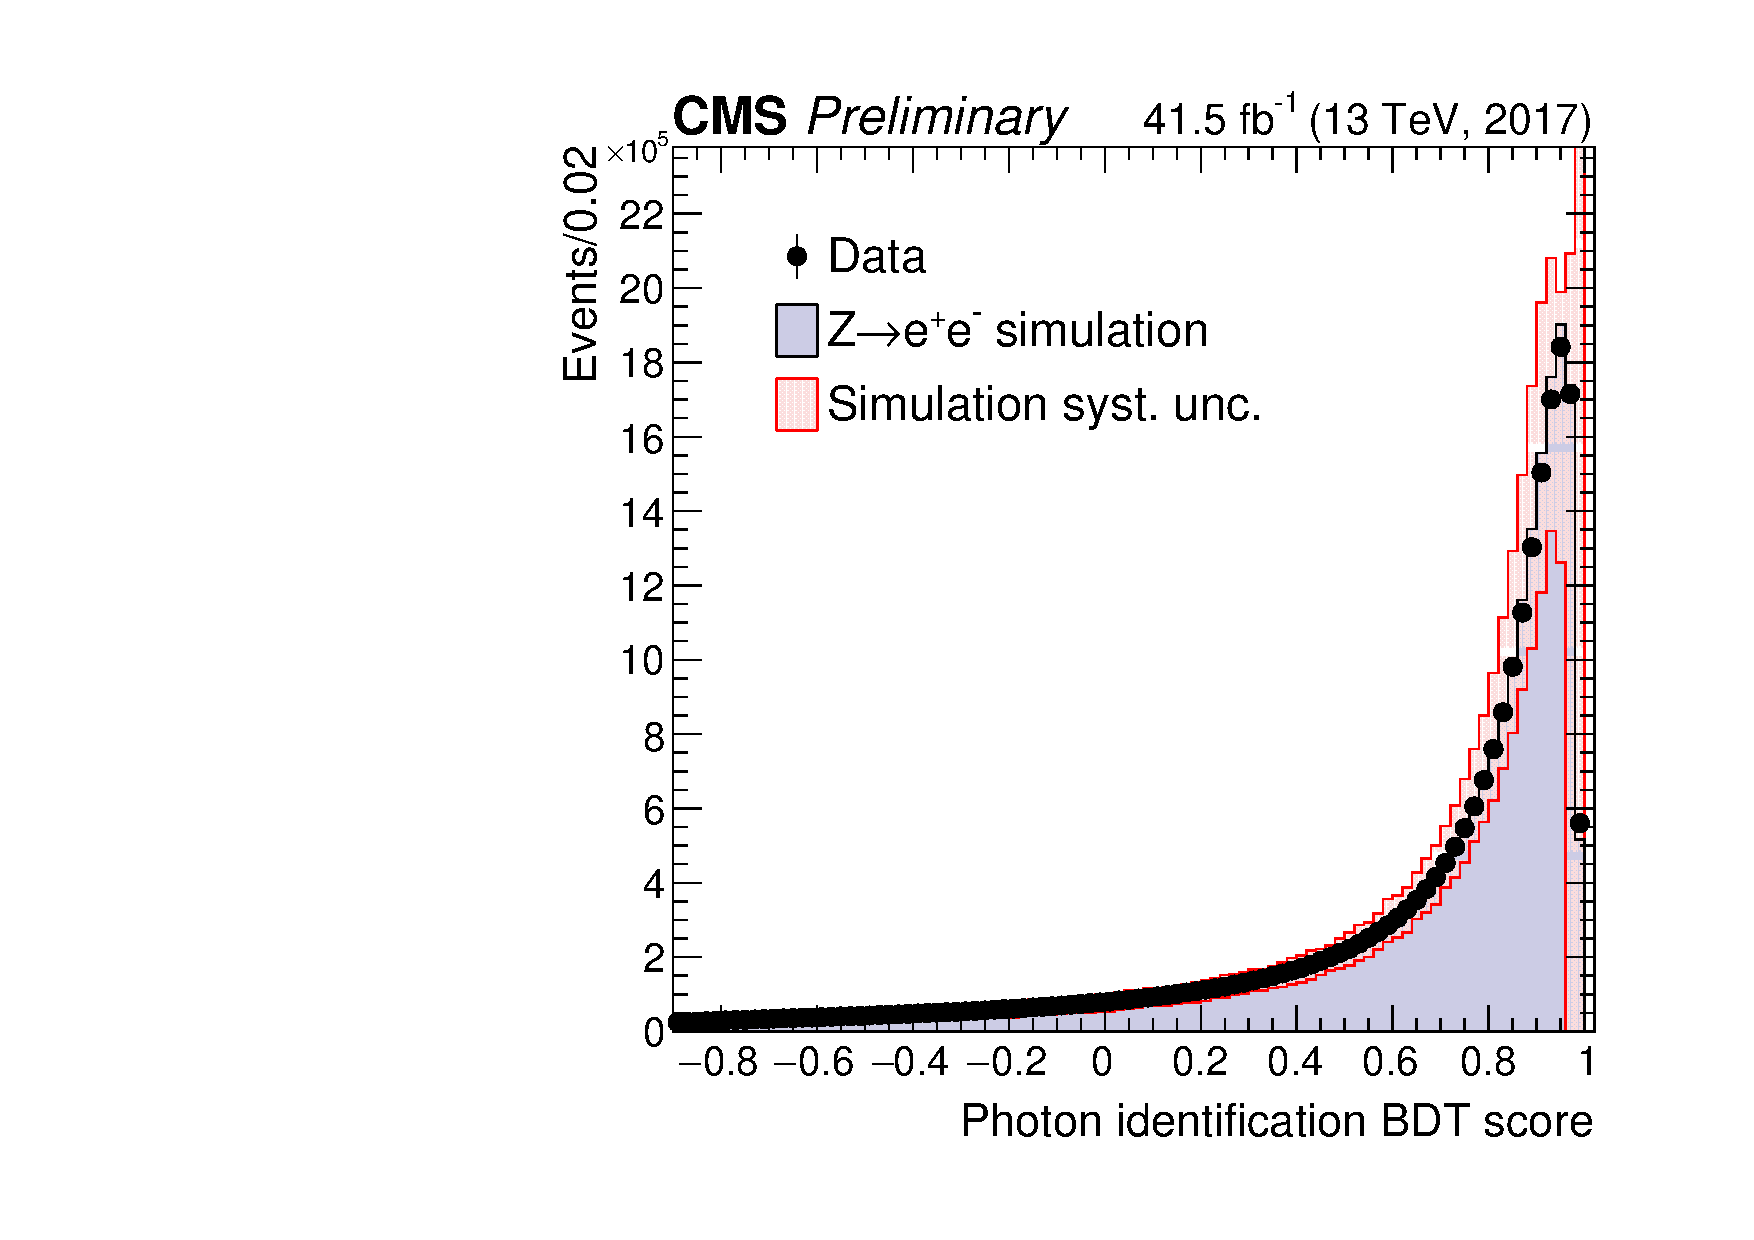
\includegraphics[width=0.49\textwidth]{Figures/Objects/ZeeIDMVA2017}
  \caption[Photon identification BDT score validation in \Zee events.]
  {
    Distribution of the photon identification BDT
    for \Zee events in data and simulation, where the electrons are reconstructed as photons. 
    The systematic uncertainty applied to the shape from simulation (hashed region) is also shown.
    The left figure shows 2016 data and simulation, with 2017 data and simulation shown on the right.
  }
  \label{fig:obj_ZeeIDMVA}
\end{figure}

\section{Vertex reconstruction}

As can be seen in Equation~\ref{eq:obj_mgg}, 
the only parameters affecting the diphoton mass are the photon energies and the opening angle between them.
Since there are multiple p-p interactions at each bunch crossing, multiple vertices are present in each event, spread along the $z$-axis.
The choice of the vertex from which the diphoton originated has a direct impact on the angle $\theta$, 
and therefore the diphoton mass resolution.
Provided the chosen vertex is within ~\SI{1}{cm} of the true interaction vertex,
the mass resolution is dominated by the photon energy resolution and the contribution from the angle is negligible.
A BDT is therefore trained to identify the most likely diphoton interaction vertex.

\subsection{Vertex selection}

The vertex identification BDT is trained with simulated \Hgg signal events, 
with the objective of selecting the true interaction vertex.
Since photons do not produce tracks, its inputs are variables related to tracks
recoiling against the diphoton system.
The variables are calculated for each candidate vertex, and are defined as follows:
\begin{itemize}
        \item $\sum_{i}|\vec{p}_T^{i}|^{2}$,
        \item $\displaystyle -\sum_{i}(\vec{p}_T^{i}\cdot \frac{\vec{p}_T^{\gamma\gamma}}{|\vec{p}_T^{\gamma\gamma}|})$,
        \item $(|\sum_{i}\vec{p}_T^{i}| - \pt^{\gamma\gamma})/(|\sum_{i}\vec{p}_T^{i}| + \pt^{\gamma\gamma})$,
\end{itemize}
where $\vec{p}_T^{i}$ is the \pt of the $i$-th track
associated with a given vertex 
and $\vec{p}_T^{\gamma\gamma}$ is the vector representing the diphoton transverse momentum.

If one or more of the photons have converted into electrons in the tracker, 
two more variables are used in addition to those above:
\begin{itemize}
        \item the number of conversions,
        \item the pull $|z_{\text{vtx}} - z_e| /\sigma_{z}$ between the
                longitudinal position of the reconstructed vertex,
                $z_{\text{vtx}}$, and the longitudinal position of the
                vertex estimated using conversion track(s), $z_e$,
                where the variable $\sigma_{z}$ denotes the uncertainty 
                on $z_e$.
\end{itemize}

The vertex with the highest vertex identification BDT output score is then chosen 
as the \Hgg interaction point.
This choice is considered to be the ``correct" vertex if the distance from the true interaction vertex
is less than \SI{1}{cm}, and is used to define the vertex choice efficiency.
The inclusive efficiency is approximately 82\% in 2016 conditions, %TODO define inclusive?
decreasing only slightly to 81\% in 2017 conditions.
This shows that the vertex identification procedure is robust to increases in pileup.
It also represents a substantial improvement compared to the default CMS vertex, %chosen using largest sum of squared track pT
which is correct in around 74\% of events.
%WV worsens resolution by about 1 GeV

The performance of the vertex identification BDT is
validated using $\Zmumu$ events.
The tracks from the muons are ignored in order to mimic the diphoton system.
Comparison between data and simulation in these events is shown in Figure~\ref{fig:obj_VtxId}.

\begin{figure}[h!]
  \centering
  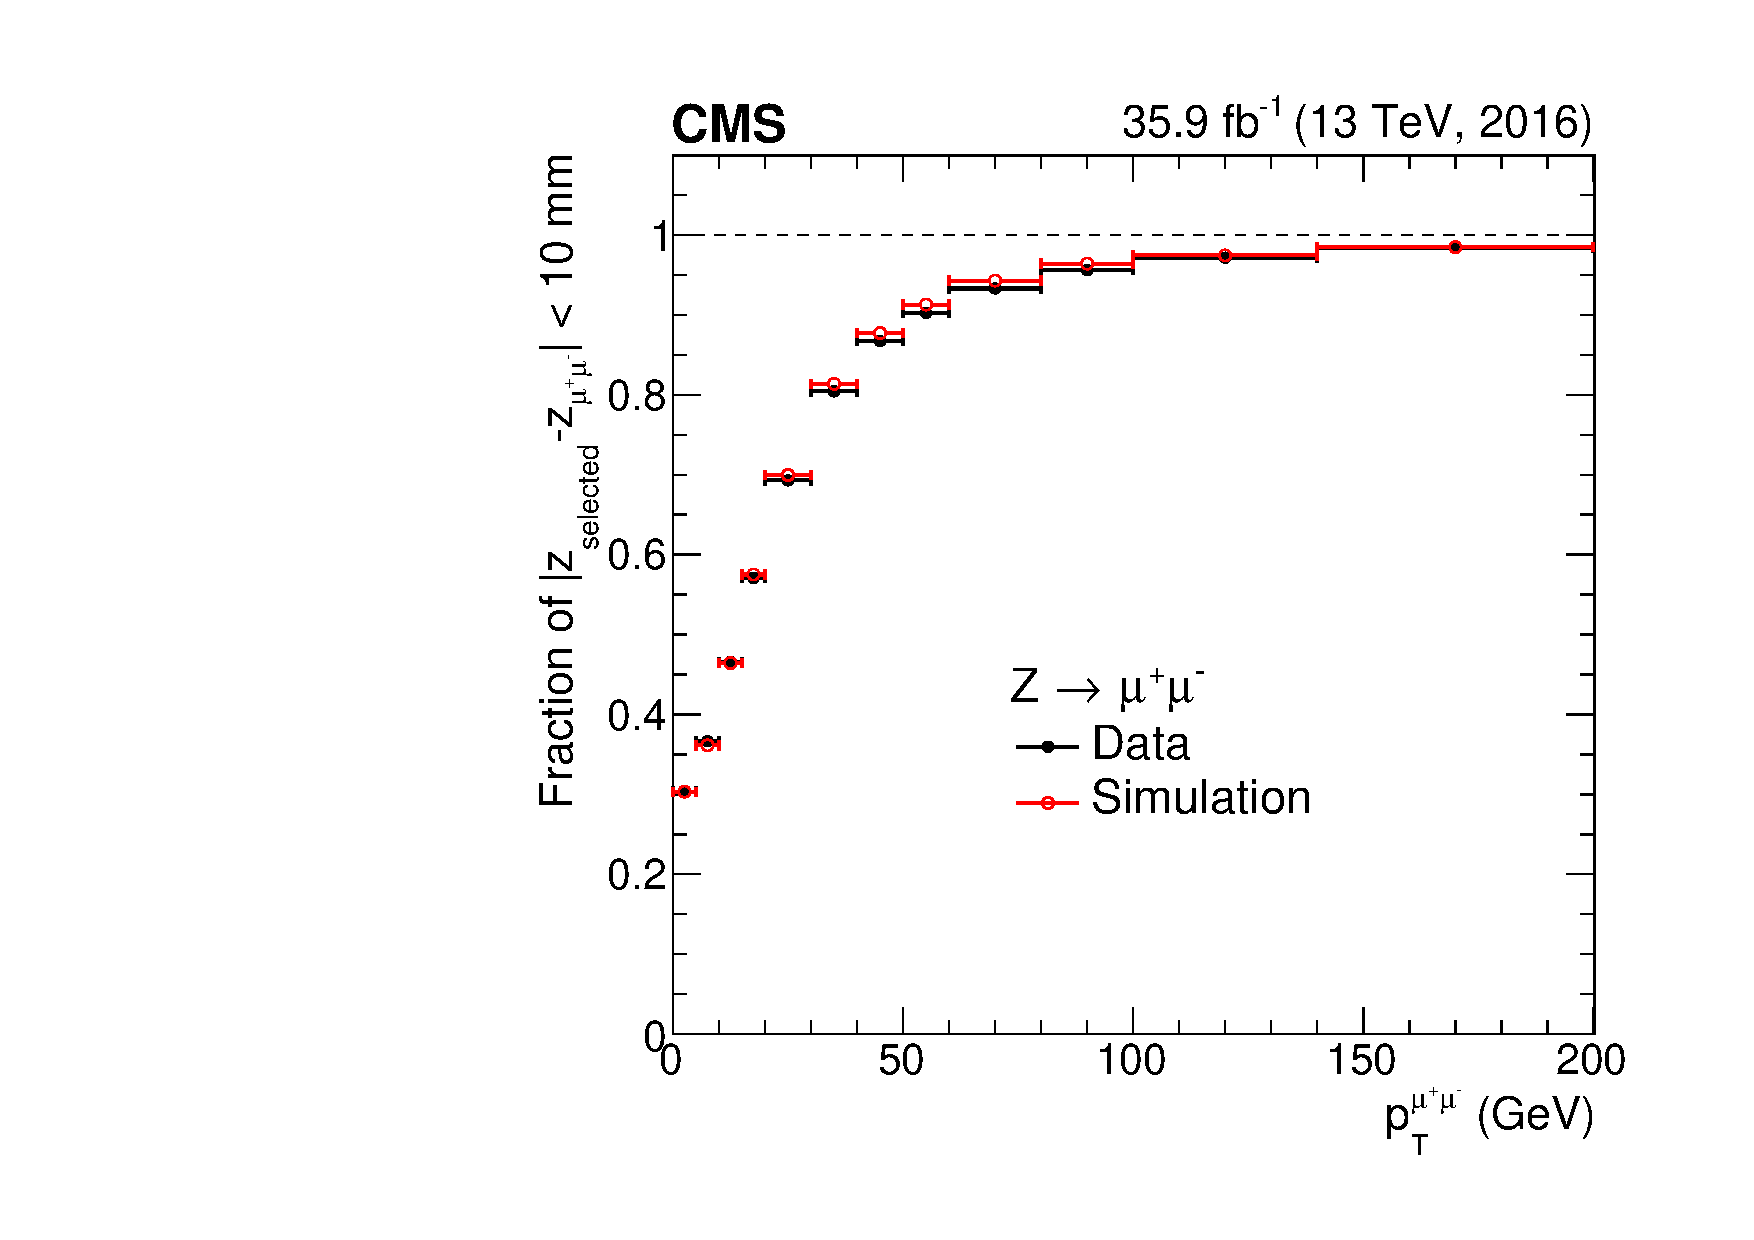
\includegraphics[width=0.49\textwidth]{Figures/Objects/VtxId2016}
  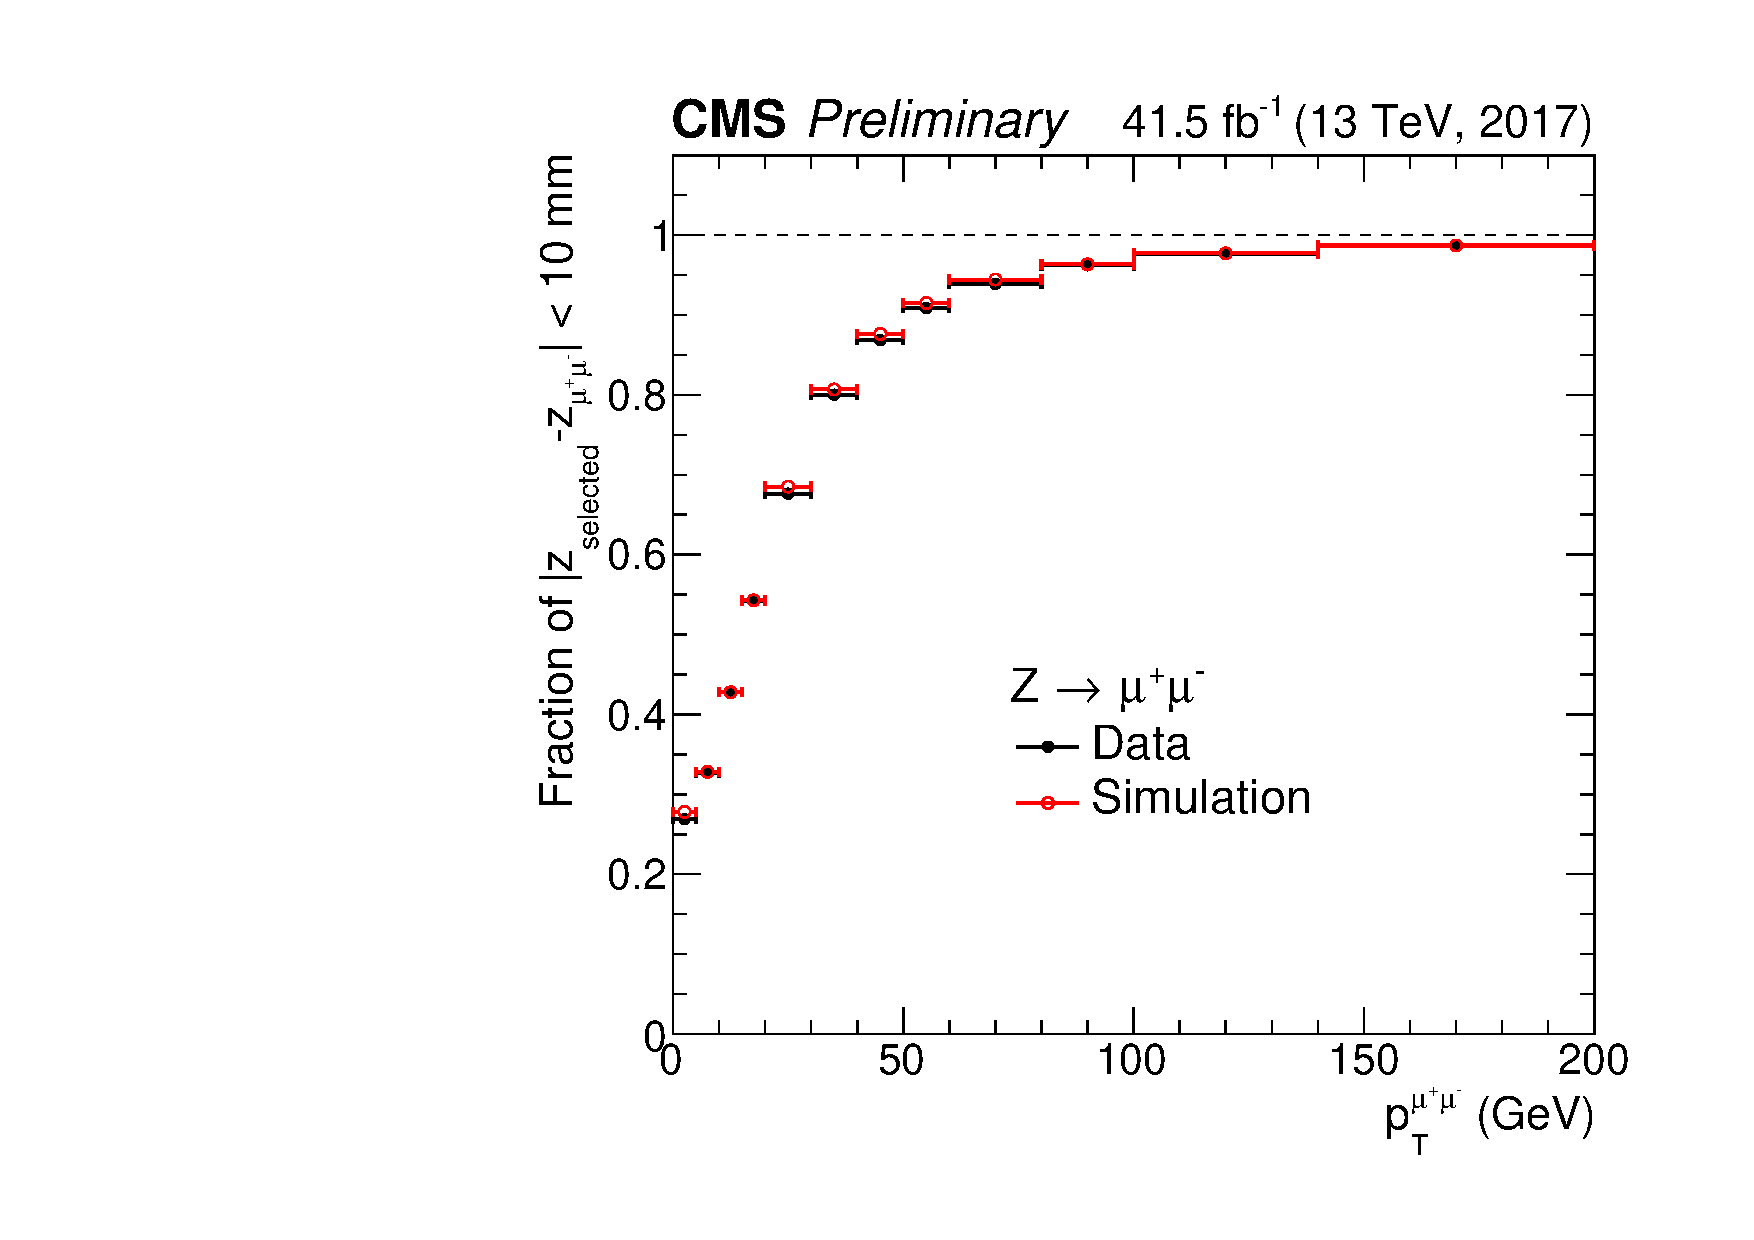
\includegraphics[width=0.49\textwidth]{Figures/Objects/VtxId2017}
  \caption[Vertex identification validation in \Zmumu events.]
  {
    Validation of the \Hgg vertex identification algorithm on \Zmumu events
    omitting the muon tracks. 
    Simulated events are weighted to match the distributions of pileup
    and location of primary vertices in data.
    The left figure shows 2016 data and simulation, with 2017 data and simulation shown on the right.
  }
  \label{fig:obj_VtxId}
\end{figure}

\subsection{Vertex probability}

A second vertex-related multivariate discriminant (vertex probability BDT),
is designed to estimate, event-by-event, the probability for the vertex
assignment to be within \SI{1}{cm} of the diphoton interaction point
and thus considered ``correct".
The vertex probability BDT is trained on simulated $\Hgg$ events using
the following input variables:
\begin{itemize}
        \item the number of vertices in each event,
        \item the values of the vertex identification BDT score for
                the three most probable vertices in each event,
        \item the distances between the chosen vertex and the second and
                third choices,
        \item the transverse momentum of the diphoton system, $\pt^{\gamma\gamma}$,
        \item the number of photons with an associated conversion track.
\end{itemize}

\begin{figure}[h!]
  \centering
  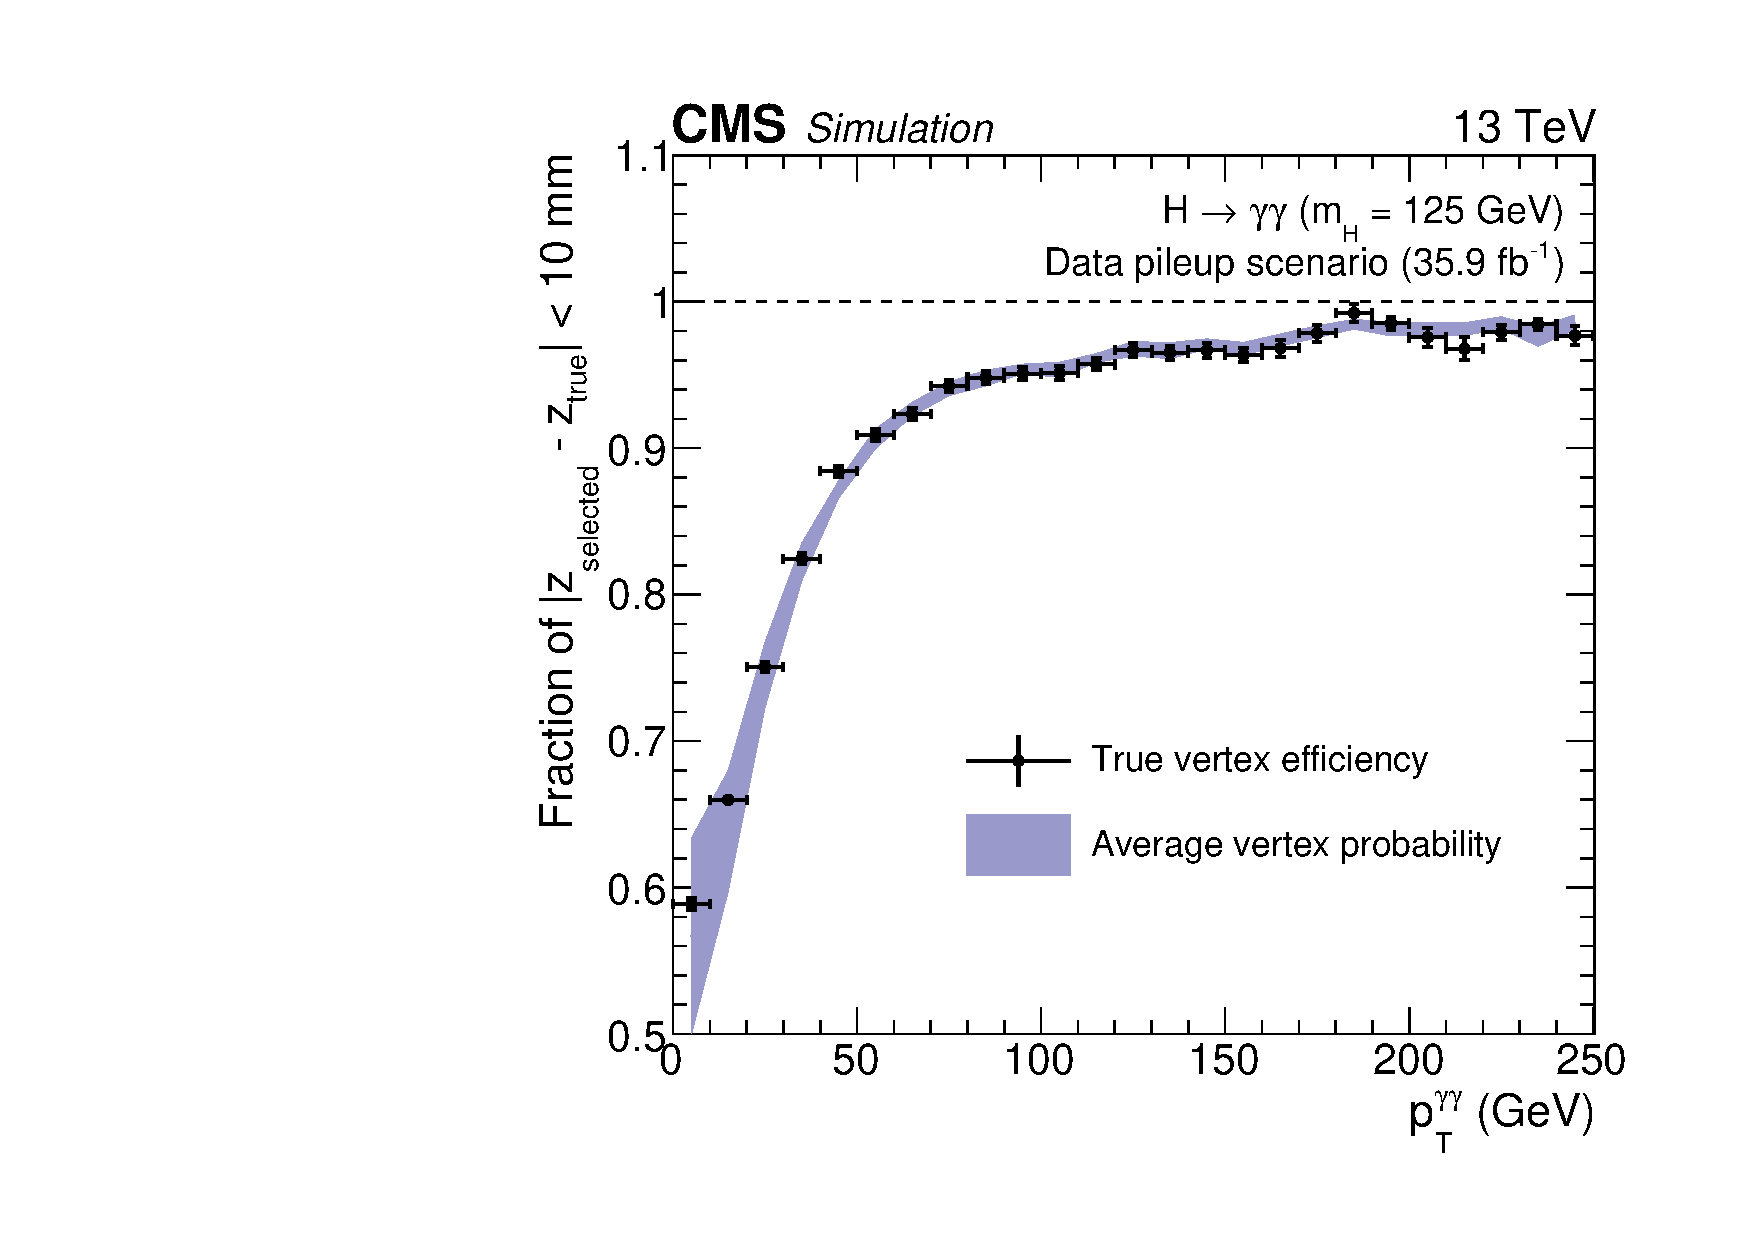
\includegraphics[width=0.49\textwidth]{Figures/Objects/VtxProbPt2016}
  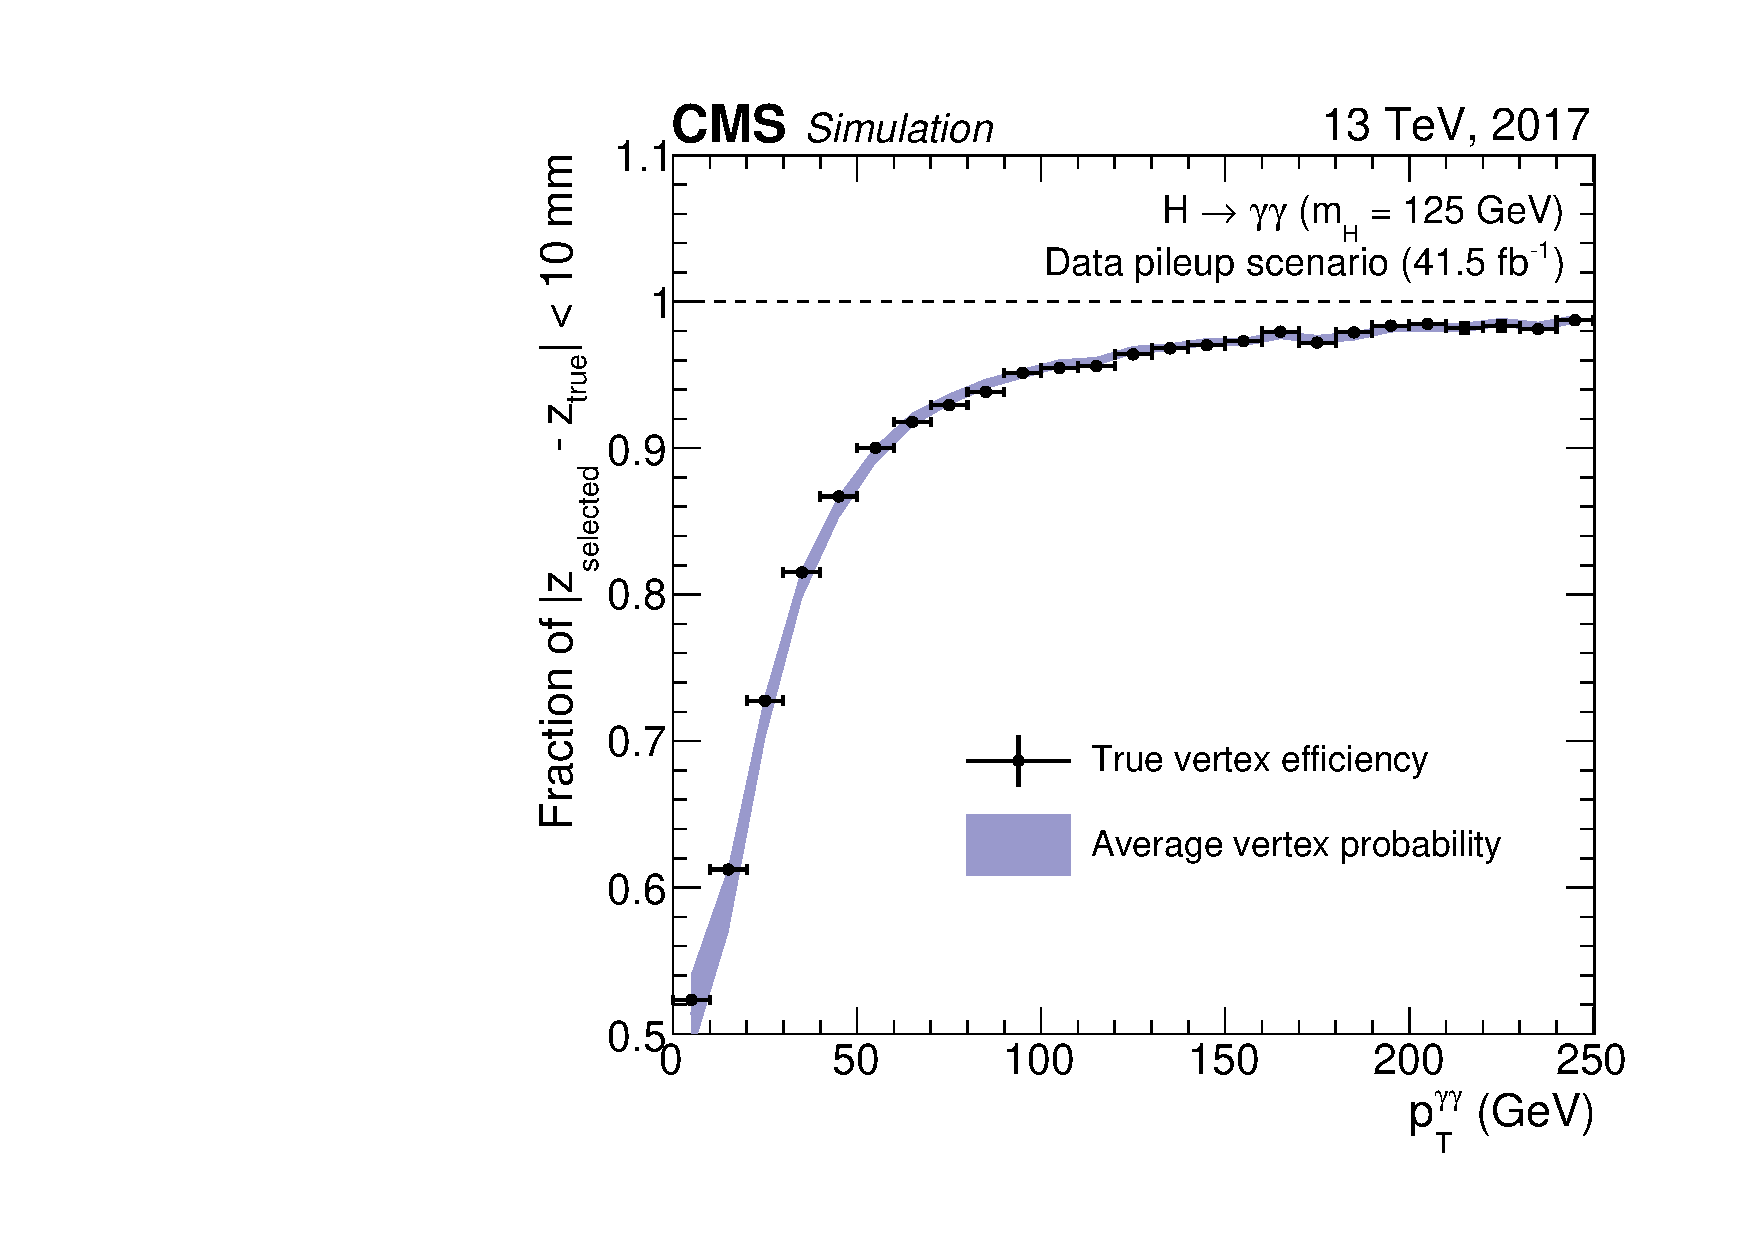
\includegraphics[width=0.49\textwidth]{Figures/Objects/VtxProbPt2017} \\
  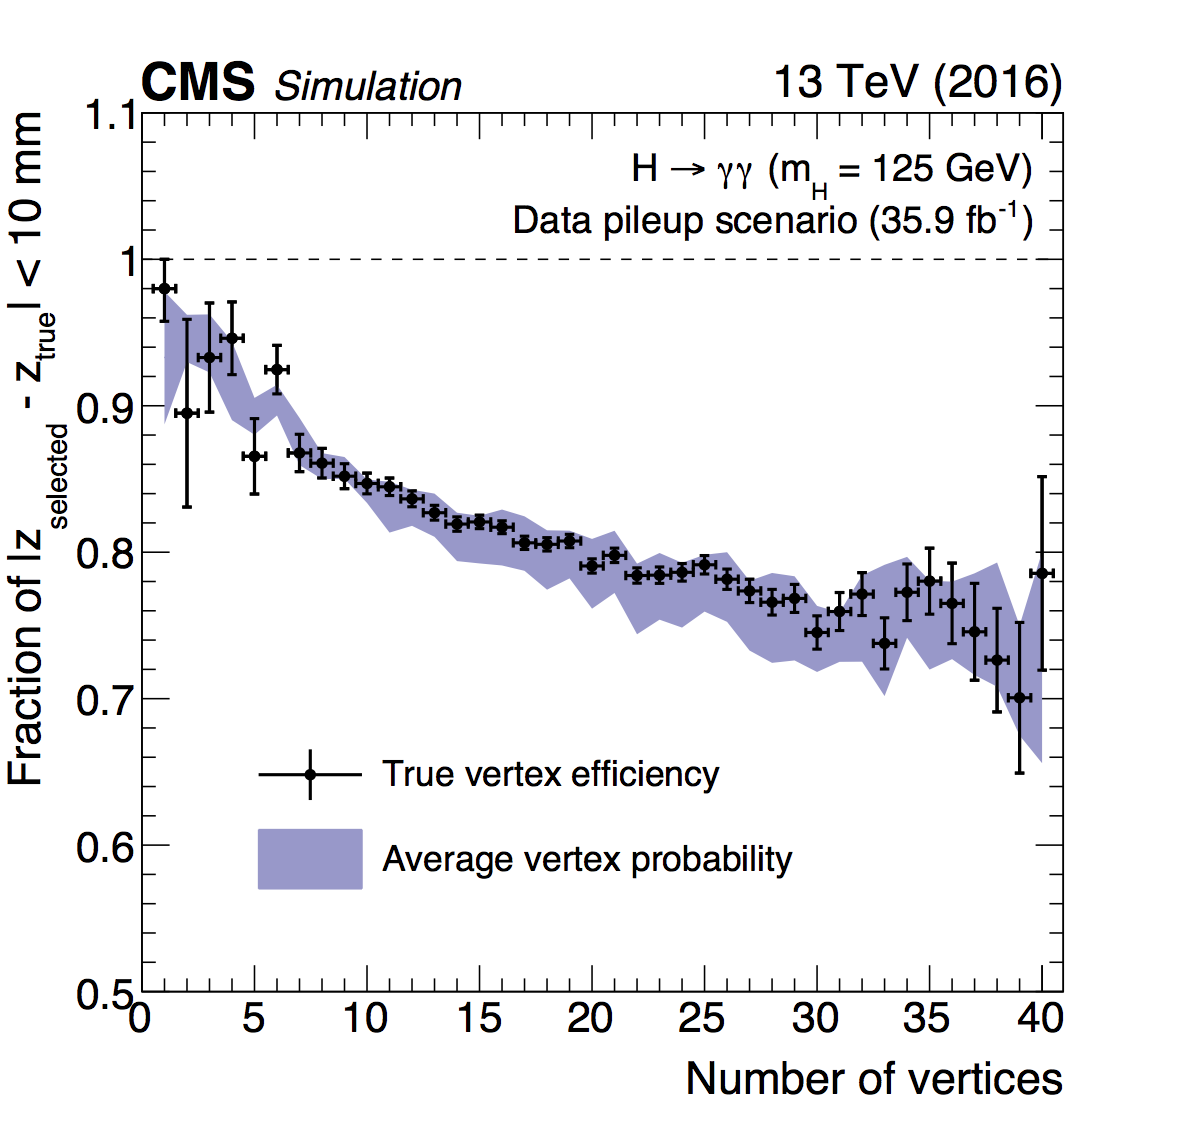
\includegraphics[width=0.49\textwidth]{Figures/Objects/VtxProbNvtx2016}
  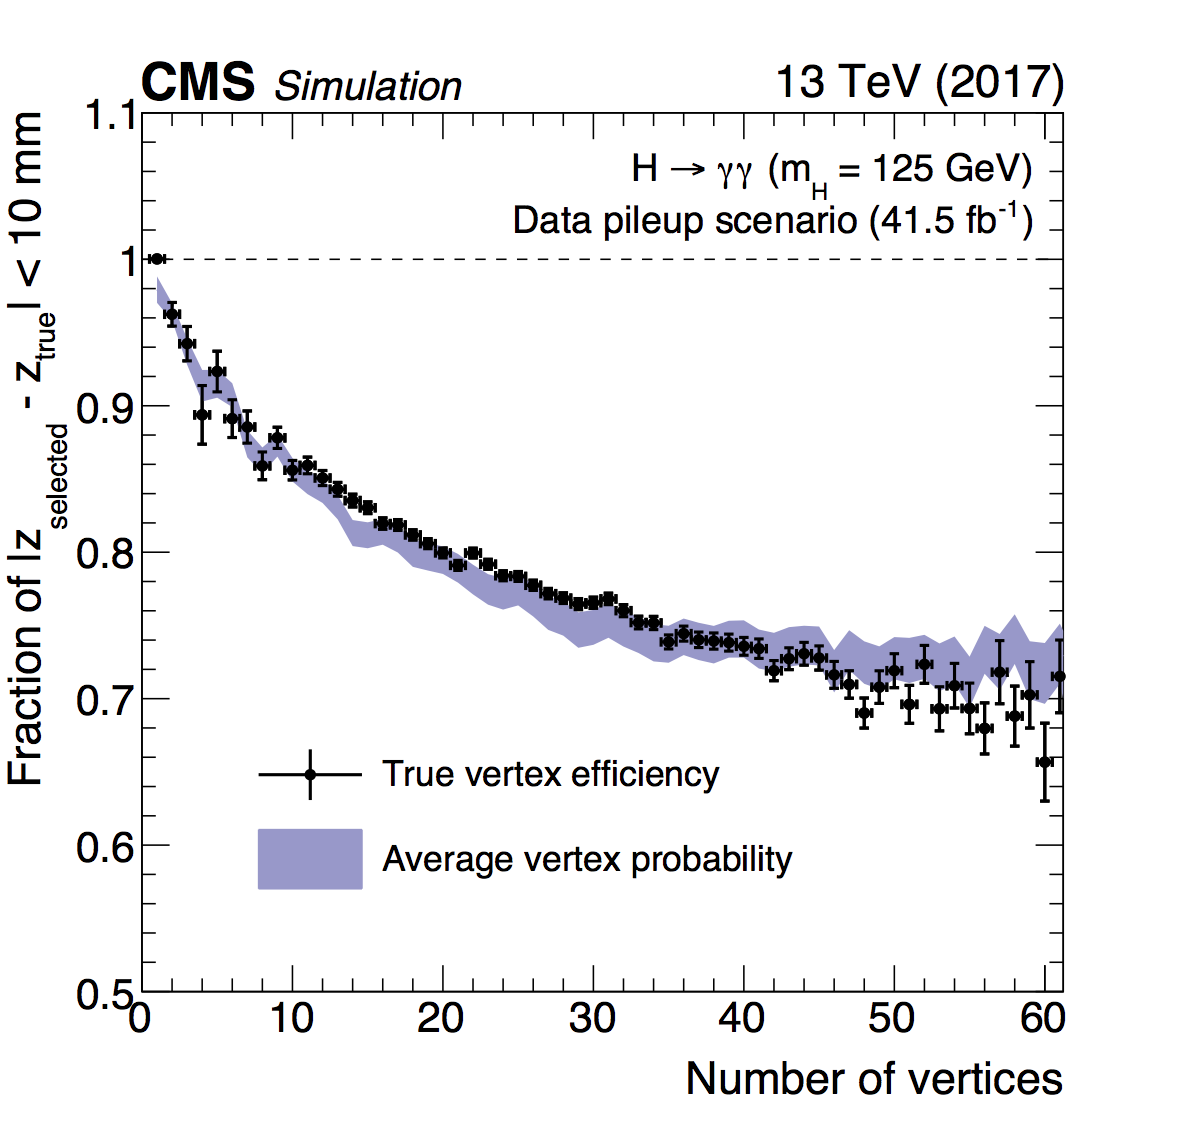
\includegraphics[width=0.49\textwidth]{Figures/Objects/VtxProbNvtx2017}
  \caption[Vertex probability validation in simulated \Hgg events.]
  {
    Comparison of the true vertex identification efficiency and the average estimated
    vertex probability as a function of the reconstructed diphoton \pt (top) and of the number of
    primary vertices (bottom) in simulated \Hgg events with $\mH = \SI{125}{GeV}$. Events are weighted
    according to the cross sections of the different production modes and to match the distributions
    of pileup and location of primary vertices in data.
    The plots on the left show simulation under 2016 conditions, 
    with simulation under 2017 conditions shown in the plots on the right.
  }
  \label{fig:obj_VtxProb}
\end{figure}

The vertex choice efficiency, together with the estimated vertex probability,
in simulated \Hgg signal events is shown in Figure~\ref{fig:obj_VtxProb}.
The simulated performance is shown as a function of both the \pt of the diphoton
system and of the number of vertices in the event.

\section{Jet reconstruction}

The collimated collection of particles produced by the hadronisation of quarks or gluons are referred to as jets.
Around 60\% of the average jet energy comes from charged hadrons, whose energy is well-measured by the tracker,
and another 30\% from photons, whose energy is measured precisely by the ECAL.
The remaining 10\% of energy from neutral hadrons is measured with worse resolution by the HCAL.
Jets are important in the \Hgg analysis because they enter the definition of the STXS signal bin definitions, 
are used to categorise the events targeting those bins, 
and are used to differentiate between production modes.

At CMS jets are formed using the \akt clustering algorithm~\cite{AntiKt} with distance parameter $R=0.4$. % check definitions of infrared and collinear safe etc
It is an iterative algorithm that defines a distance metric dependent on the \pt and angular parameters of candidate clusters of energy deposits, 
and groups together these clusters starting with the nearest two objects.
Once the shortest distance is between an object and the beampipe, the process stops and the clustered objects defined as a jet.
This is then repeated until all clusters have been collected into jets.

The inputs to the \akt algorithm are PF candidates with charged hadron subtraction (CHS)~\cite{JEC}. 
CHS reduces the contribution from pileup by identifying any charged hadrons associated with vertices other than the primary vertex.
Since the tracker coverage extends only to $|\eta|=2.5$, 
jets further forward than this do not have pileup removed via CHS.
Once the jets have been constructed, a set of corrections are applied to correct the jet energy scale and resolution in both data and simulation.
The correction procedure can be summarised as~\cite{JEC}:
\begin{itemize}
  \item corrections are made for the pileup contribution to jets, as a function of the event energy density, 
        and the jet \pt, $\eta$ and area.
        Any remaining differences between data and MC are derived after these corrections using pileup-only events.
  \item the reconstructed jet energy is corrected to agree with the true jet energy in both data and MC.
        This is performed as a function of \pt and $\eta$ to account for variation in response across the detector.
  \item residual differences between data and MC are corrected in two steps.
        First $\eta$-dependent corrections are applied using dijet events, 
        where the scale of a jet is corrected using a jet of similar \pt in the reference, well-measured $\eta < 1.3$ region.
        The \pt-dependent corrections are derived using events with a jet recoiling against a photon or $Z$ boson.
        This corrects the absolute scale of the jet.
  %\item finally, corrections dependent on the jet flavour are applied.%state optional? if not look up
\end{itemize}
%The final uncertainties on the jet energy scale are below 3% across the phase space considered
%by most analyses (pT > 30 GeV and |η| < 5.0). In the barrel region we reach an uncertainty
%below 1% for pT > 30 GeV, when excluding the jet-flavor uncertainties, provided separately
%for different jet-flavor mixtures. At its lowest, the core uncertainty 
%(excluding optional timedependent and flavor systematics) is 0.32% for jets with pT between 165 and 330 GeV, and |η| < 0.8. 

Additional selection can be applied to these calibrated jets to further reject jets originating from pileup.
Pileup jets are typically more dispersed than real jets, since they do not have an energetic core generated by a parton.
A pileup jet identification BDT is therefore trained using jet shape variables, 
and additional track variables related to the interaction vertex of the jet.
The output score of this BDT is used to reject pileup, with thresholds dependent on the \pt and $\eta$ of jets.
For a jet to be considered in the analysis, it must pass the pileup jet identification and have $\pt > \SI{30}{GeV}$ and $|\eta| < 4.7$.

\section{Reconstruction of other objects}

Additional objects can be used to specifically target rarer Higgs boson production modes, such as $VH$ and $ttH$.
Whilst not used directly in this analysis, they are important in both Refs~\cite{HIG-16-040} and \cite{HIG-18-018}.

\subsection{Muons}

Muons can be produced in the decays of $W$ or $Z$ bosons arising in $VH$ events.
The reconstruction of muons can be seeded either by tracks found in the muon system, 
or by tracks from the inner tracker that are extrapolated to the muon system, or both.
Identification criteria ensuring the muon is isolated, 
applied by checking that the \pt and tracks and calorimeter deposits are consistent with the \pt of the muon track, 
reduces the mis-identification of other charged hadrons.
The energy is inferred from the curvature of the inner track for $\pt < \SI{200}{GeV}$.
Above this value, additional information from the muon tracks is used to accurately fit the track
and improve the precision of the \pt measurement.
A full description of the muon reconstruction is givn in Ref.~\cite{MuonReco}.


\subsection{Electrons}

Similarly to muons, electrons can be present in leptonic $VH$ decays.
Electrons are reconstructed in a very similar way to photons, 
but requiring, instead of vetoing, a matching track.
They can be seeded either by calorimeter deposits or tracks.
The energy measurement is performed using a BDT similar to that photons, 
but which also incorporates track information and further accounts for energy lost by bremsstrahlung.
Further detail on the electron reconstruction is available in Ref.~\cite{ElectronReco}.

\subsection{Missing transverse momentum}

The presence of neutrinos in an event can be inferred by a global imbalance in the vector sum of the \pt of all objects, 
resulting in so-called ``missing" transverse momentum (\met).
The \met computation uses the corrected \pt values for objects, and with all jet energy corrections applied.
It can be used to identify the neutrinos resulting from $W$ boson decay in $VH$ events.

\chapter{Event Categorisation}
\label{chap:categorisation}

\section{Introduction}

The analysis event selection consists of the preselection described in Chapter~\ref{chap:objects}, 
and in addition requires the two leading preselected photon candidates to have 
$\pt^{\gamma 1} > \mgg/3$ and $\pt^{\gamma 2} > \mgg /4$ respectively, 
with an invariant mass in the range $100\,<\,\mgg\,<\,\SI{180}{GeV}$.
The requirements on the scaled photon transverse momenta prevent distortions 
at the lower end of the mass spectrum.
Both photons must also satisfy the
pseudo-rapidity requirement $|\eta|\,<\,2.5$ and must not be in the barrel-endcap
transition region $1.44\,<\,|\eta|\,<\,1.57$;
the reduced containment in this transition region worsens the photon energy resolution.
The above $\eta$ requirement is applied to the photon supercluster
position, and the requirement on the photon $\pt$ is applied 
after the vertex assignment.

The \Hgg analysis depends on the ability to distinguish the narrow signal peak 
from the smoothly falling background in the diphoton mass distribution. 
Selected events are therefore subject to further categorisation, in order to 
increase the ratio of the number of signal events to the number of background events (S/B).
This enhances the sensitivity of the analysis, 
reducing the expected uncertainties on the measured quantities.

Analysis categories are also constructed to target events in which the Higgs boson was 
produced by a specific production mechanism. 
This is achieved using the information provided by additional objects in the event, 
alongside the two photons arising from the Higgs boson decay.
As well as facilitating measurements of cross sections corresponding 
to individual production mechanisms, these dedicated categories also enable the S/B to be improved.

In the previous \Hgg analysis using the 2016 dataset \cite{HIG-16-040}, 
dedicated categories targeting the VBF, ttH, and VH modes were constructed, 
with the remaining so-called ``Untagged" categories composed mostly of ggH events.
Here a similar approach is employed, 
but with additional divisions targeting individual stage 1 bins for the ggH and VBF processes.

The dataset collected by CMS in 2017 has already been used in an analysis targeting ttH production,
which is described in Ref.~\cite{HIG-18-018}.
In order to ensure that the set of data events included in this analysis is orthogonal 
from those included in Ref.~\cite{HIG-18-018}, 
a veto is applied to events selected for categories targeting ttH production.
The criteria used to select ttH include two dedicated BDTs, 
one targeting events where at least one W boson decays leptonically
and the other preferentially selecting fully hadronic W boson decays.
Input variables to the two BDTs include photon, lepton, and jet kinematics, 
information relating to $b$-tagging, and missing transverse momentum.
The veto is implemented by applying these criteria used to construct the ttH categories, 
and then removing them from further consideration. 
Around fifteen events are expected to be removed as a result, 
most of which would otherwise have populated the ggH 2J categories with higher \ptH values.
Furthermore, there are no dedicated analysis categories for VH production; 
there are insufficient statistics in the diphoton decay channel with this dataset 
to measure any of the individual stage 1 bins~\cite{YR4}.

The categorisation targeting ggH is based on the reconstructed diphoton transverse momentum (\ptgg) 
and the number of jets in the event. 
A BDT referred to as the diphoton BDT is then used to reduce the amount of background. 
The VBF analysis categories make use of the same diphoton BDT 
to reduce the number of background events. 
Additionally, a BDT targeting the kinematics of the characteristic VBF dijet system, 
known as the dijet BDT, is utilised to reduce the contamination from ggH events.

Due to conditions differing between the two years, 
the analysis is optimised separately for the 2016 and 2017 datasets. 
A simultaneous fit to the categories from both years is then performed to estimate the 
values of the parameters of interest and their uncertainties (described in Chapter ~\ref{chap:results}).
The following section provides an introduction to BDTs and how they are used in physics analyses.
The remainder of the chapter then describes in detail the training of the diphoton and dijet BDTs, 
and their use in the category optimisation process for both ggH and VBF events.

\section{Boosted decision trees}
\label{sec:BDTs}
In the CMS \Hgg analysis, BDTs are used for several purposes.
Generally, the purpose of the BDT is to discriminate between 
one signal-like and one background-like process.
The BDT provides a per-event output score which indicates how signal-like the event is, 
and a criterion can be applied on this output score when selecting or categorising events.
This section gives a brief explanation of what BDTs are and how they are trained.

A BDT is an example of a machine learning algorithm which takes as input a set of features, 
a set of training parameters, and a loss function, 
and from those inputs returns an output score~\cite{ElementsLearning}.
The so-called feature vector $\vec{x}$ is a set of real values for each event
which can be used to discriminate between signal and background processes. 
Examples of features used in the analysis include kinematic variables such as \pt or $\eta$.
In addition, when training the BDT, the target outcome $y$ must be provided.
The events used for training typically come from simulation, where the truth process is known.
For all the cases considered in this analysis, $y$ simply takes the value 1 for signal events
and 0 for background events.
The training parameters $\vec{w}$, also referred to as hyper-parameters, 
are parameters which control the behaviour of the learning procedure.
The loss function $L$ defines the metric on which the learning procedure is optimising.
The output score for events being evaluated is denoted $Y$.

A BDT is an ensemble of decision trees (DTs), 
which are so-called base learners that recursively split the input feature space into distinct regions
by applying binary partitions at each node.
Once a given branch reaches its final node where no further splitting is performed, 
an output value is assigned to that region.
The training procedure for an individual DT involves considering many possible configurations
for the tree and computing the loss function for each one.
The point at which the training process terminates depends upon the hyperparameter values.
For example, there may be a restriction on the tree depth, 
meaning the number of binary partitions permitted for each branch.
In this way an optimal configuration is chosen, 
and any given input for evaluation (without the target label $y$) 
will be placed in a single region and assigned the corresponding score.

The boosting procedure combines individual DTs into a more powerful learner.
An iterative training process enables the existing models to be improved upon, 
by each new learner corrects the previous one.
The final BDT output function then consists of a weighted sum of individual DTs.
A type of boosting method known as gradient boosting trains each successive tree 
on the residuals, or errors, of the existing function, 
thereby attempting to correct the mistakes made by existing trees.
This is equivalent to subtracting the derivative of a squared error loss function;
this is the reason the method is given the name gradient boosting.
This gradient boosting procedure can be generalised to use pseudo-residuals, 
which are given by the derivative of an arbitrary differentiable loss function.
The loss function chosen here is distinct from that used to train the individual DTs.
Once a new tree is trained on these pseudo-residuals, it is then added to the existing function, 
itself a weighted sum of trees.
The weight of the new tree is assigned by minimising the loss of the new summed function.
This procedure is repeated until a given performance threshold or other stopping criterion is met.

The performance of a given BDT training is evaluated on a sample independent 
of that used to train it, in order to ensure that 
the features learned by the BDT generalise beyond the specific training dataset used.
If the BDT's performance is greater on the training dataset than the so-called test dataset, 
it is said to have overfitted, or been overtrained.
This means it has placed too much importance on statistical fluctuations on the training dataset
which will not be present in other samples.
The hyperparameters chosen for a given training will affect whether or not the BDT is overtrained.
For example, the learning rate reduces the weight assigned to each tree in the iterative learning
process, which is analogous to the step size in gradient descent methods.
A smaller learning rate will reduce the chance of overfitting 
but also increase the time taken for the training to converge.
For this reason, an optimisation procedure is normally used to choose the hyperparameters
in such a way that maximises performance without overtraining the BDT.

\section{Gluon fusion categorisation}
\subsection{Signal bin definitions}

At stage 1 of the STXS framework, 
the gluon fusion process (ggH) is divided into a total of eleven particle level bins.
The events are split first by the number of jets, 
defined at particle level using the anti-$k_T$ algorithm with radius parameter 0.4 
and jet $\pt > \SI{30}{GeV}$~\cite{AntiKt}.
All stable particles except for the decay products of the Higgs boson 
are included in the anti-$k_T$ clustering.
There are zero (0J), one (1J), and greater than or equal to two (2J) jets bins.
In events with at least one jet, a further splitting 
by the value of the transverse momentum of the Higgs boson (\ptH) is performed. 
Four bins are defined by boundaries placed at 60, 120, and \SI{200}{GeV}.
These bins are denoted as low, medium (med), high, and BSM, respectively.
Finally, a separate ggH region is dedicated to the vector boson fusion-like phase space, 
for which a pair of jets (a dijet) with invariant mass $m_{jj} > \SI{400}{GeV}$ 
and difference in pseudorapidity $\Delta\eta > 2.8$ is required.
The dijet is formed from the two leading jets in the event.
This region is split into two-jet-like ($\ptHjj < \SI{25}{GeV}$) 
and three-jet-like ($\ptHjj > \SI{25}{GeV}$) bins, 
where \ptHjj is defined as the transverse momentum of the Higgs boson plus dijet system.
Each bin is exclusive; events included in the VBF-like region are not included in the other ggH 2J bins.
A table summarising the definition of each bin, its cross section, and the fraction of the 
total ggH cross section is shown in Table \ref{tab:cat_ggHfractions}.
The inclusive ggH cross section is $48.52~\textrm{pb}$ at $\mH = \SI{125.09}{GeV}$, 
computed to an accuracy of three loops in perturbative QCD 
and next-to-leading order (NLO) in EW perturbations~\cite{YR4,Anastasiou2015,Anastasiou2016}.
Approximately $44.2~\textrm{pb}$ of this is within $|y_H| < 2.5$.

\begin{table}
  \begin{centering}
    \begin{tabular}{ r | c | c | c } 
\hline
\multirow{2}{*}{Region}      & \multirow{2}{*}{Definition}                             & \multirow{2}{*}{Fraction} & Cross \\ 
                             &                                                         &                           & section (pb) \\ 
\hline
0J                           & Exactly zero jets, any $\ptH$                           & 60.0\%                    & 26.49 \\ 
\hline
1J low                       & Exactly one jet, $\ptH <$ 60 GeV                        & 15.4\%                    & 6.79  \\
\hline
1J med                       & Exactly one jet, 60 $< \ptH <$ 120 GeV                  & 10.4\%                    & 4.61  \\ 
\hline
1J high                      & Exactly one jet, 120 $< \ptH <$ 200 GeV                 & 1.7\%                     & 0.76   \\
\hline
1J BSM                       & Exactly one jet, $\ptH >$ 200 GeV                       & 0.4\%                     & 0.16   \\ 
\hline
2J low                       & $\ge$ two jets, $\ptH <$ 60 GeV                         & 2.9\%                     & 1.26   \\
\hline
2J med                       & $\ge$ two jets, 60 $< \ptH <$ 120 GeV                   & 4.5\%                     & 2.00   \\ 
\hline
2J high                      & $\ge$ two jets, 120 $< \ptH <$ 200 GeV                  & 2.3\%                     & 1.00   \\
\hline
2J BSM                       & $\ge$ two jets, $\ptH >$ 200 GeV                        & 1.0\%                     & 0.43   \\ 
\hline
\multirow{2}{*}{VBF-like 2J} & $\ge$ two jets, $\ptH < 200$ GeV, $|\Delta\eta| > 2.8$, & \multirow{2}{*}{0.6\%}    & \multirow{2}{*}{0.27} \\ 
                             & $m_{jj} >$ 400 GeV, $\ptHjj <$ 25 GeV                   &                           & \\ 
\hline
\multirow{2}{*}{VBF-like 3J} & $\ge$ two jets, $\ptH < 200$ GeV, $|\Delta\eta| > 2.8$, & \multirow{2}{*}{0.9\%}    & \multirow{2}{*}{0.38} \\ 
                             & $m_{jj} >$ 400 GeV, $\ptHjj >$ 25 GeV                   &                           & \\ 
\hline
\end{tabular}

    \caption[Particle level definitions of the ggH stage 1 STXS bins.]
    {
      The particle level definition of each ggH stage 1 bin 
      and the corresponding fractional and absolute cross sections.
      The fractions are estimated from simulated ggH \Hgg events 
      within the region $|y_H| < 2.5$.
      Details of the simulated samples can be found in Chapter~\ref{chap:objects}.
      Each bin is exclusive; 
      events included in the VBF-like region are not included in the other ggH 2J bins.
    }
    \label{tab:cat_ggHfractions}
  \end{centering}
\end{table}

\subsection{Categorisation strategy}

In order to measure the stage 1 bins individually, 
categories must be constructed which differentiate between them.
Thus the reconstruction level event categorisation is designed to target all of the bins 
to which some sensitivity can be obtained in the \Hgg decay channel with this dataset.
In this case, the majority of the ggH stage 1 bins can be measured individually. 
The exceptions are the two VBF-like bins, 
which are difficult to separate from true VBF production.
Therefore events not entering the categories targeting VBF production 
can be assigned to one of nine target ggH stage 1 bins.
This assignment is performed using the reconstructed 
diphoton transverse momentum (\ptgg) and the number of jets -- 
which are respectively the detector level equivalents 
of the particle level quantities \ptH and number of jets used to define the bins.
The same boundaries are used as for the particle level bins; 
0, 60, 120 and \SI{200}{GeV} in \ptgg for 1J and 2J events, 
and inclusive in \ptgg for 0J events.
%More advanced assignment procedures have been studied, 
%and show modest improvement with respect to this version; 
%these are described in Chapter~\ref{chap:conclusion}
Once a target signal bin has been assigned, 
the diphoton BDT is used to further divide the events into up to three categories.
Requirements are placed on the output score of the diphoton BDT, 
with the category with the highest threshold referred to as ``Tag 0", 
the next highest as ``Tag 1", and so on.
This reduces the amount of background 
and therefore improves the analysis' sensitivity to each ggH stage 1 bin.

\subsection{Diphoton BDT}

The diphoton BDT is trained to discriminate signal events 
(where two photons are produced from the decay of a Higgs boson) from background events 
(where two photons are produced by other SM processes).
The goal of the classifier is to assign high scores to signal-like events;
requirements can then be placed on the output score of the classifier 
to increase the S/B for the analysis categories.
The criteria for an event to be signal-like include having signal-like photon kinematics, 
and having high scores from the photon identification BDT.
In addition, events with a good diphoton mass resolution are preferred 
since this reduces the amount of background present under the signal peak.

To train the diphoton BDT, simulated events from the ggH, VBF, ttH 
and VH production modes are treated as signal. 
The event generator used for training the BDT (\textsc{POWHEG}) 
is different from that used to construct the final signal model.
This ensures that the final results are not biased by re-using the same events.
Simulated background events include the contributions from prompt-prompt, prompt-fake, 
and fake-fake sources.
For both signal and background, 
events are weighted in accordance with the SM process cross section.
Furthermore, events from the QCD sample are down-weighted by a factor of 25;
the limited number of events in this sample results in very high per-event weights, 
which causes the classifier to over-estimate the importance of individual events.
All events are required to satisfy the analysis selection criteria.
The input variables to the classifier are the kinematic properties of the diphoton system, 
a per-event estimate of the diphoton mass resolution, 
and the photon identification scores of each photon.
The set of input variables is chosen such that the value of the Higgs boson mass cannot be inferred;
it is for this reason that the photon momenta are divided by the diphoton mass.
The full list of input variables is as follows:
\begin{itemize}
\item the transverse momentum of the two leading photons, divided by the diphoton mass, $\pt^{1,2}/\mgg$;
\item the pseudorapidity of the two leading photons, $\eta^{1,2}$;
\item the cosine of the angle between the two photons in the transverse plane, $\cos{(\Delta\phi)}$;
\item the output score of the photon identification BDT for the two leading photons;
\item the per-event relative mass resolution estimate, 
      under the hypothesis that the mass was computed using the correct primary vertex \srv/\mgg;
\item the per-event relative mass resolution estimate, 
      under the hypothesis that the mass was computed using an incorrect primary vertex \swv/\mgg;
\item the per-event probability estimate that the correct primary vertex was selected, $p_{vtx}$,
      which is the output of the vertex probability BDT described in Chapter~\ref{chap:objects};
\end{itemize}

The per-event relative mass resolution under the correct vertex hypothesis 
depends only on the photon energy measurements performed by the ECAL.
It is calculated by propagating the photon energy resolution estimates, 
assuming the resolutions are independent and Gaussian distributed:

\begin{equation}
  \srv/\mgg = \frac{1}{2} \sqrt{\left(\frac{\sigma_{E_1}}{E_1}\right)^{2}
                              + \left(\frac{\sigma_{E_2}}{E_2}\right)^{2}}
\end{equation}

where both the energy ($E_{1,2}$) and energy resolution ($\sigma_{E_{1,2}}$) estimates 
are obtained from the regression described in Chapter~\ref{chap:objects}.
Under the incorrect vertex hypothesis, an additional term must be added to account for the 
worsening in the diphoton mass resolution due to the uncertainty of the vertex position.
The distance between the correct and incorrect vertices is assumed to follow a Gaussian distribution
with a width dependent on the size of the beamspot.
The contribution from the vertex ($\sigma_{vtx}$) can then be computed analytically 
using the measured positions of the photons in the detector 
and combined in quadrature with \srv to calculate \swv:
%TODO understand this better

\begin{equation}
  \swv/\mgg = \sqrt{\left(\frac{\srv}{\mgg}\right)^{2}
                              + \left(\frac{\sigma_{vtx}}{\mgg}\right)^{2}}
\end{equation}

An example of the distribution for one of the input kinematic variables, the lead photon $\pt/\mgg$, 
is shown in Figure~\ref{fig:cat_ptominput}.
The background, split into its prompt--prompt, prompt--fake, and fake--fake components, 
is compared to the data sidebands (where the region with $115 < \mgg < \SI{135}{GeV}$ is excluded).
Good agreement between the two is observed.

\begin{figure}[hptb]
  \centering
  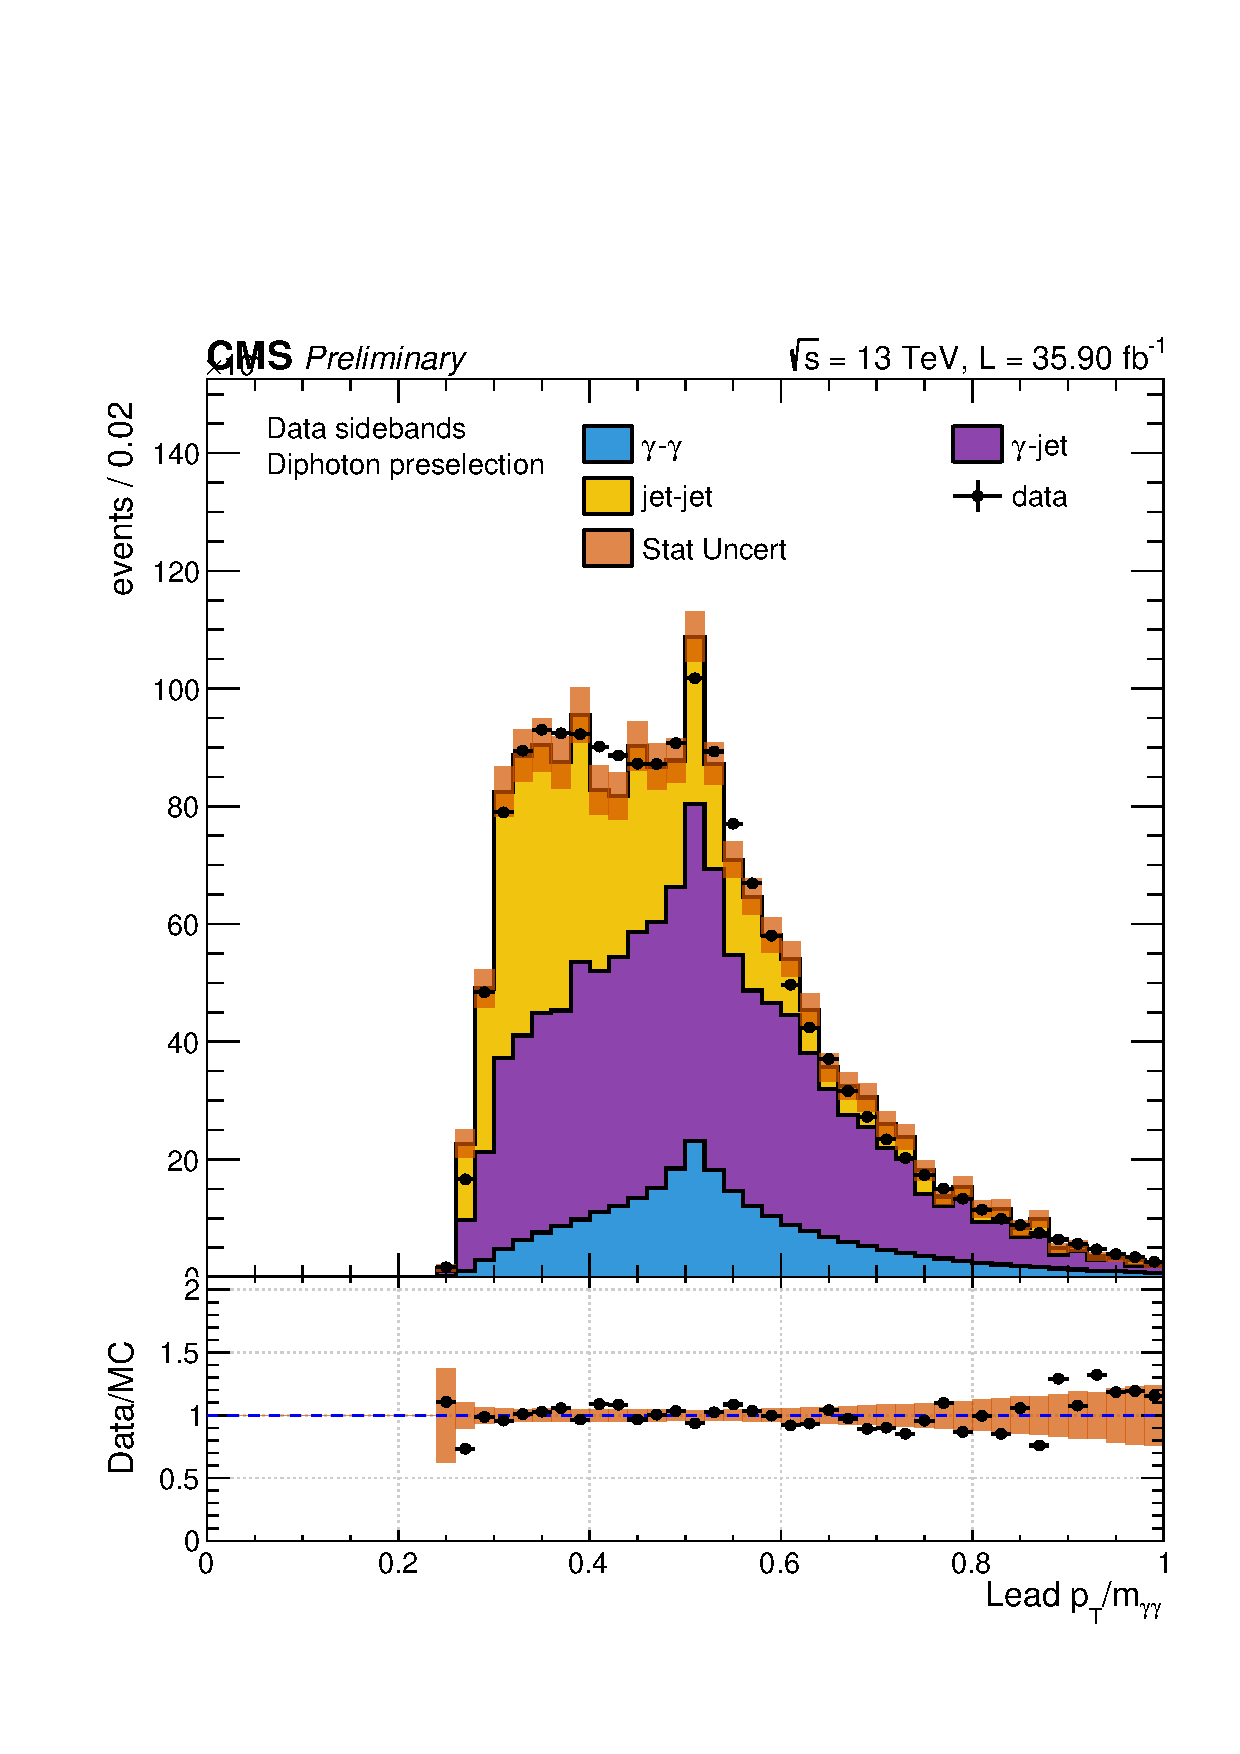
\includegraphics[width=0.49\textwidth]{Figures/Categorisation/leadptom_2016.pdf}
  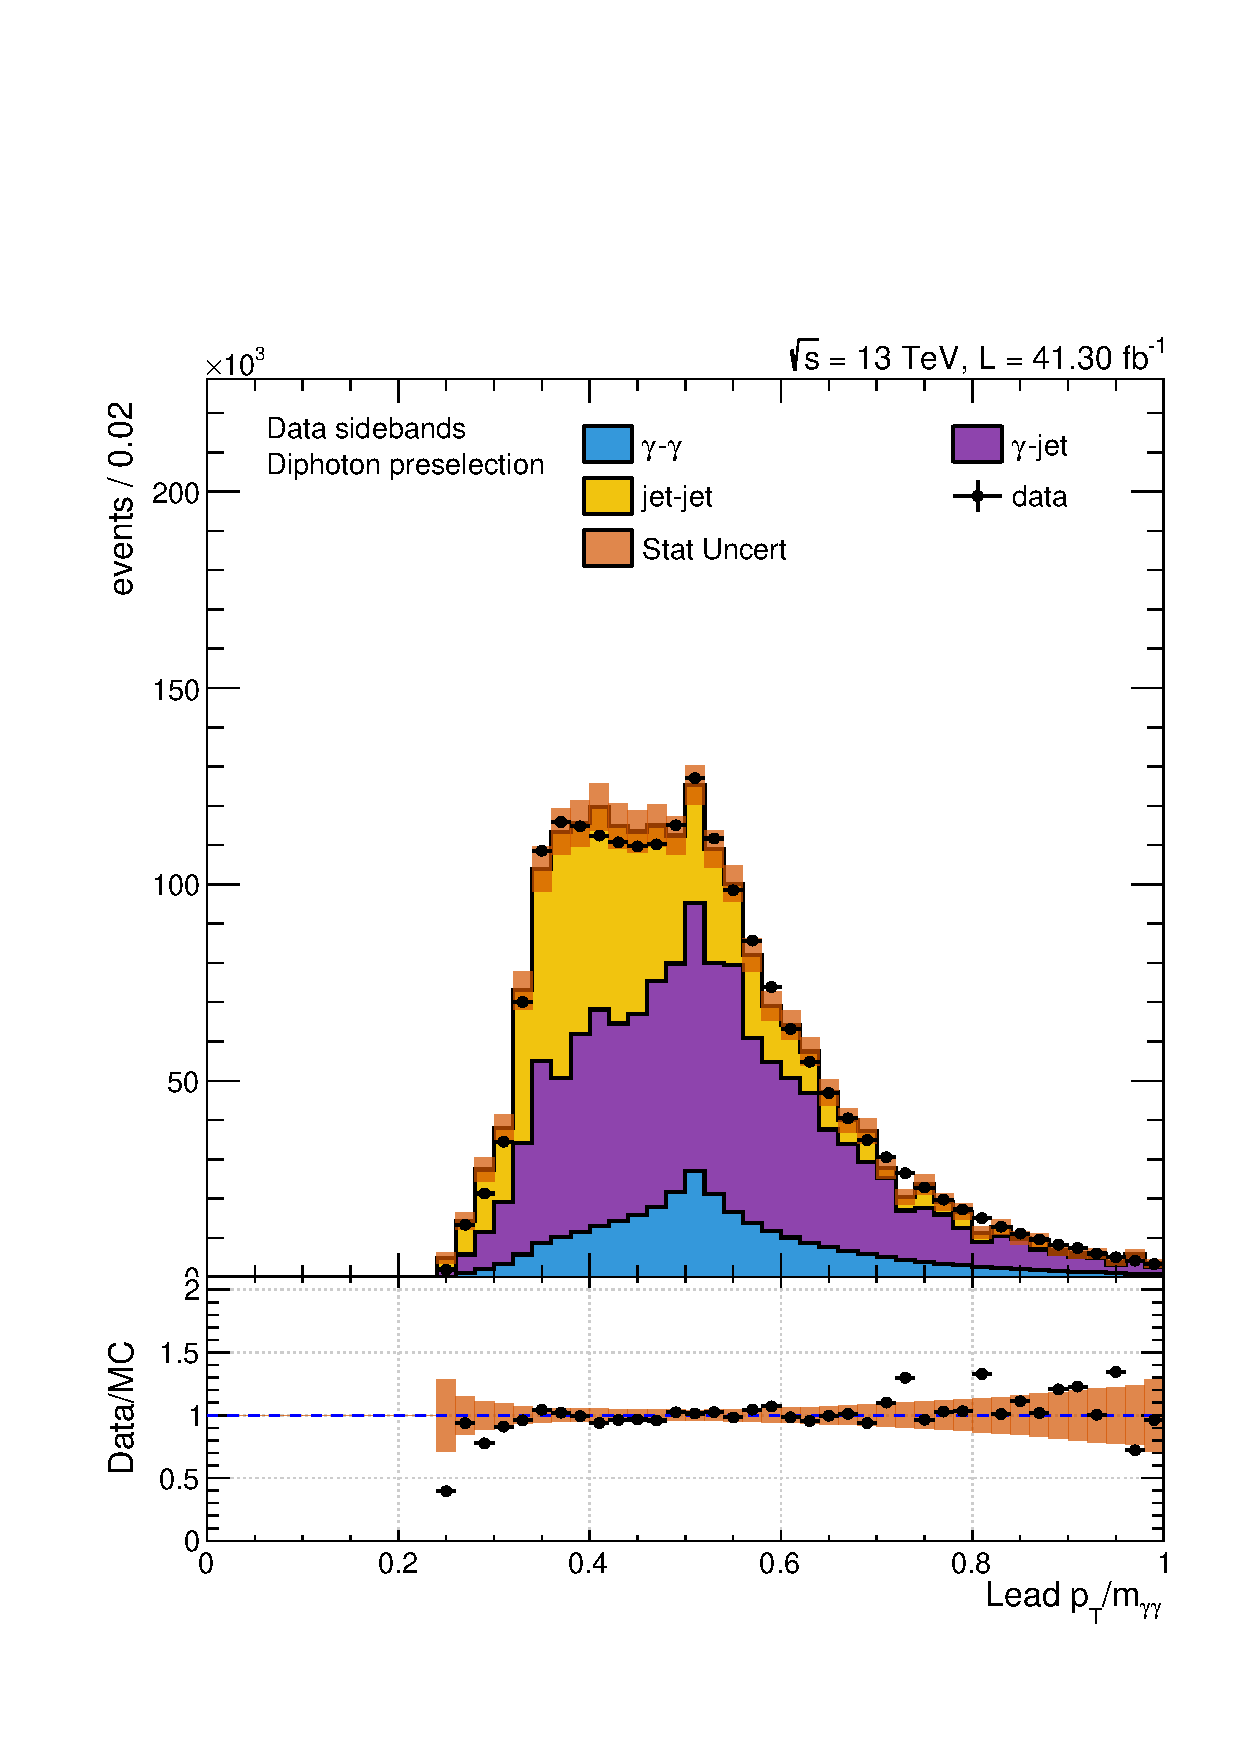
\includegraphics[width=0.49\textwidth]{Figures/Categorisation/leadptom_2017.pdf}
  \caption[Leading photon scaled \pt distributions.]
  {
    Distribution of the leading photon $\pt/\mgg$ in background (stacked histogram) 
    and data (black points) events.
    The statistical uncertainty is shown by the orange band.
    The left plot shows 2016 data and MC,
    with 2017 data and MC on the right.
  }
  \label{fig:cat_ptominput}
\end{figure}

None of the input variables above encode the preference for events with good mass resolution.
For this purpose, an additional weight is applied to signal events which increases the relative 
importance of events with better values of the diphoton mass resolution. 
The weight applied, $w_{res}$, is given by the formula

\begin{equation}
  w_{res} = \frac{p_{vtx}}{\srv} + \frac{1-p_{vtx}}{\swv}
\end{equation}

This ensures that the classifier output score is higher for events 
which have a relatively low expected diphoton mass resolution.
Finally, the signal and background samples are divided into a training and a test set,
containing 70\% and 30\% of the total number of events respectively.
With this configuration of input variables, signal and background events, and event weights, 
the classifier is trained and its performance evaluated using the XGBoost software package~\cite{XGBoost}.

The performance of the training is evaluated using a receiver operating characteristic (ROC) curve, 
where the signal efficiency is plotted as a function of the background efficiency,
with each point corresponding to a specific threshold value placed on the classifier output score.
The area under the ROC curve is used to gauge the performance of a given classifier; 
a higher area corresponds to more effective discrimination between signal and background.
For the 2016 and 2017 trainings, the areas under the respective ROC curves are both equal to 0.85.

This metric is utilised to compare the performance of the classifier training 
with different values of the BDT's so-called hyper-parameters.
These hyper-parameters are parameters of the BDT, 
which are not learned but instead affect how the learning algorithm behaves.
The most important hyper-parameters affect the extent to which 
the algorithm learns the specific detail of the training sample provided.
To check for potential overtraining, the training score as measured by the area under the ROC curve 
of the training set is compared with the score from the independent test set.
If the test set score is significantly higher than that of the training set, 
the classifier has been overtrained.
The default classifier hyper-parameters display no overtraining.
A coarse hyper-parameter optimisation procedure is then performed, 
in which each hyper-parameter is varied individually.
No significant improvement without overtraining is found, 
and therefore the default training parameters are used.

An additional parameter which can be optimised is the relative weight 
of the signal and background samples.
With the default sample weights corresponding to the SM sample cross section, 
the two classes are highly imbalanced.
This imbalance can cause suboptimal learning in the classifier.
To check this, the classifier is trained in a scenario 
where the signal event weights are increased by a uniform factor, 
such that the total sum of weights for signal and background is equal.
This is purely a technical change to the training 
designed to improve the learning outcomes of the classifier.
When evaluating the performance, the default event weights are used.
Equalising the total weights in this way results in a modest improvement in performance.
The areas under the ROC curves become 0.87 for both the 2016 and 2017 datasets.
The improvement is relatively small, 
but is however larger than the variation 
in training performance induced by either changing the random seed used for training or 
choosing different subsets of the input data for training and testing.
Therefore we choose to use this training scenario for the final classification.
The hyper-parameter optimisation procedure was repeated 
and no significant improvement was obtained.

%The ROC curves for the two different event weighting scenarios are shown in Figure~\ref{fig:cat_ROCs}.
%It is evident that the scenario with equalised weights has slightly superior performance.
%In addition, the relative importance of each feature is shown in Figure~\ref{fig:cat_importance}.
%This plot serves as validation that the classifier is learning 
%sensible features of the input dataset.
%TODO add ROC curve and feature importance plots here?

Validation of the diphoton BDT is performed using \Zee events, 
where simulated Drell-Yan events are compared with data.
This validation is important because although the background model used in the analysis 
is entirely data-driven, the signal model is taken from simulation.
Therefore it is necessary to ensure that there is reasonable agreement 
between data and simulation for signal-like objects,
for both the inputs to the diphoton BDT and the output score itself.
In this \Zee control region, the electrons are reconstructed as photons, 
and the presence of an electron pair with invariant mass $80 < m_{ee} < \SI{100}{GeV}$ is required.
Otherwise the event selection is the same as the analysis selection for diphoton events, 
except for the additional requirement that the leading electron $\pt > \SI{40}{GeV}$.
This requirement is necessary to ensure that no bias is introduced by the electron trigger, 
which has selection thresholds at $\pt = \SI{32}{GeV}~(\SI{35}{GeV})$ for 2016 (2017) data.

Figure~\ref{fig:cat_diphoBDT} shows the output score of the diphoton BDT for data and simulation.
The effect of two systematic uncertainties which affect the diphoton BDT are included;
these are the shift in the photon identification BDT score, 
and the uncertainty on the photon energy resolution (see Chapter~\ref{chap:sigbkg} for details).
Good agreement is observed between the data and simulation in both years, 
with all discrepancies covered by the statistical and systematic uncertainties.

\begin{figure}[hptb]
  \centering
  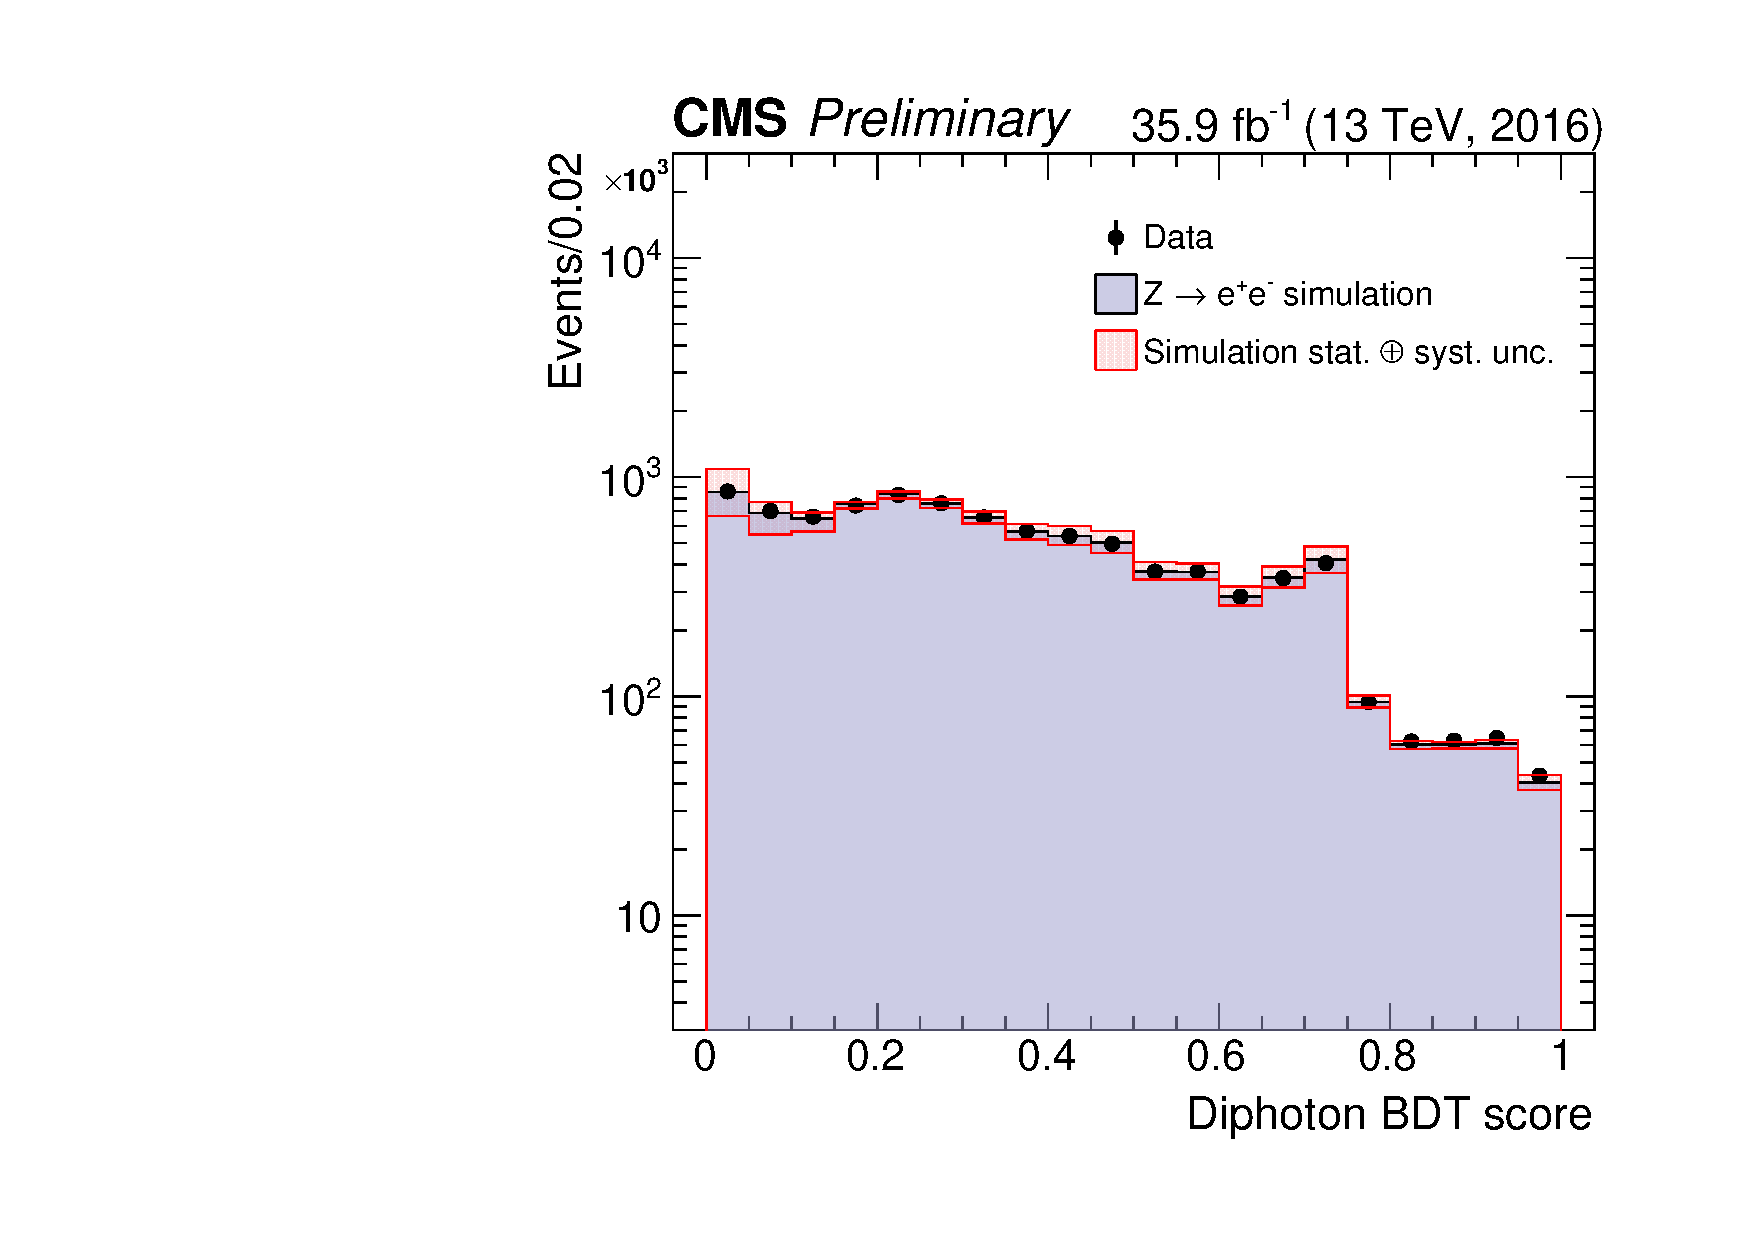
\includegraphics[width=0.7\textwidth]{Figures/Categorisation/DiphoBDT_2016.pdf}
  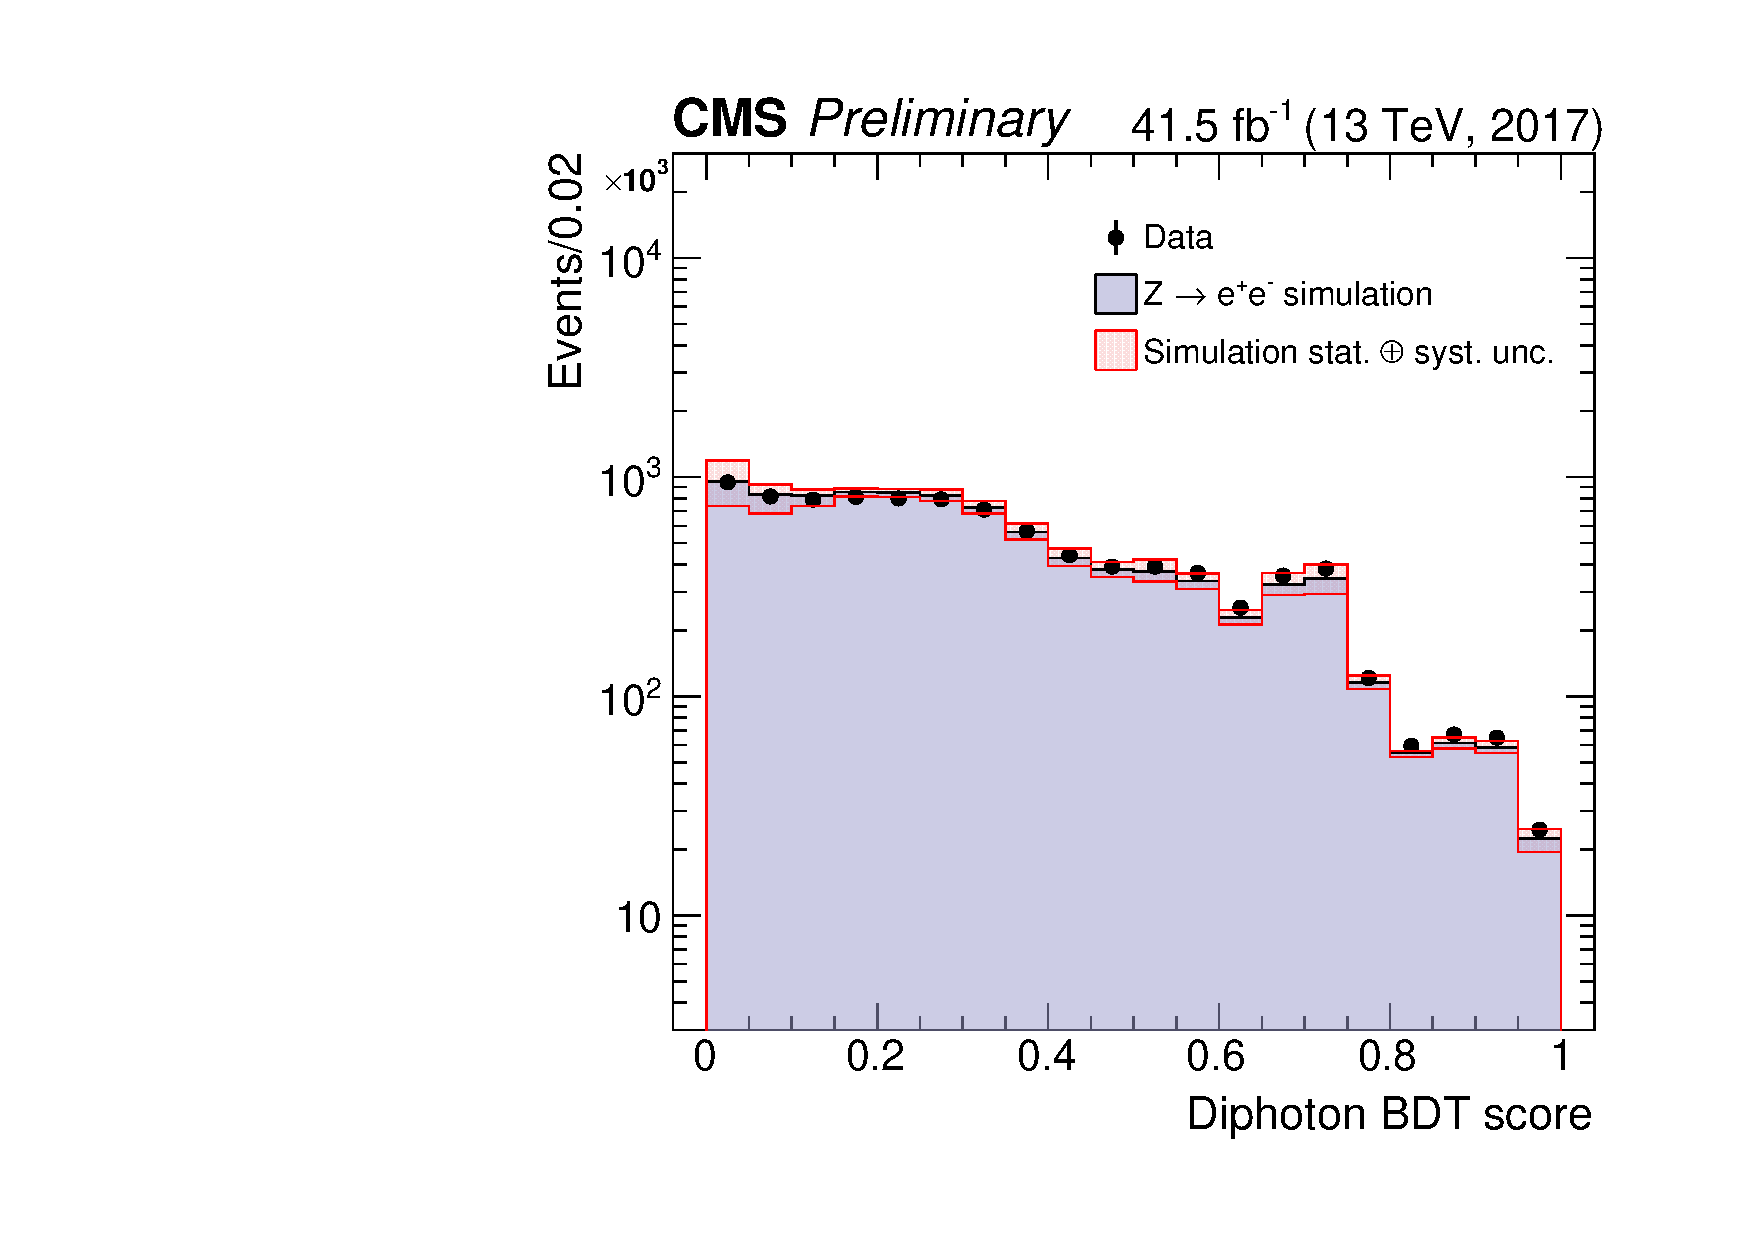
\includegraphics[width=0.7\textwidth]{Figures/Categorisation/DiphoBDT_2017.pdf}
  \caption[Validation of the diphoton BDT in \Zee events.]
  {
    Score of the diphoton BDT in $\Zee$
    events where the electrons are reconstructed as photons.
    The points show the score for data, the histogram shows
    the score for simulated Drell--Yan events, including statistical and 
    systematic uncertainties (pink band).
    The top plot shows 2016 data and MC,
    with 2017 data and MC on the bottom.
    Figures first shown in Ref.~\cite{HIG-18-029}.
  }
\label{fig:cat_diphoBDT}
\end{figure}

\subsection{Category definitions}

Once the diphoton BDT has been constructed, 
a category optimisation procedure can be performed for each Stage 1 bin independently.
The reconstructed number of jets and \ptgg define the category type into which a given event falls.
Then, independently for each category type, 
an optimisation procedure is performed to define diphoton BDT boundaries 
for a given number of subcategories.
The Approximate Mean Significance (AMS) is used to define the figure of merit for the optimisation.
The value of the AMS metric corresponds to the expected significance of a signal 
from the likelihood ratio statistic for a simple counting experiment, 
neglecting the impact of systematic uncertainties.
Its derivation is outlined in Ref.~\cite{Asymptotic}.
The aim of this analysis is not to maximise the significance of each stage 1 bin.
Maximising the AMS is instead a proxy for minimising the expected uncertainty for a given bin.
The formula for the AMS for a given analysis category is given by 

\begin{equation*}
  AMS = \sqrt{ 2 \left( (S+B) \ln{\left(1+\frac{S}{B}\right)} - S \right) }
\end{equation*}

where $S$ is 68\% (corresponding to $\pm 1\sigma_{eff}$) of the number of signal events 
from the desired truth bin (not the total number of signal events), and $B$ is the background.
The value of B is calculated by performing an exponential fit to the background, 
and then integrating the number of events between $125 - \sigma_{eff} < \mH < 125 + \sigma_{eff}$.
This formula reduces to $S/\sqrt{S+B}$ in the limit of small $S/B$.
Results are found to be robust to the choice of metric; 
only in bins with a very low number of events (e.g. the BSM bins) 
does the AMS metric return different optimal diphoton BDT boundaries from the $S/\sqrt{S+B}$ metric, 
and then the differences are relatively small.
The total AMS significance is computed by summing the values for each analysis category in quadrature.

The optimisation procedure itself is performed using a random search. 
%This is found to be more computationally efficient than a grid search.
After the diphoton BDT boundaries have been established, 
a cross-check is performed to ensure that a sensible minimum has been found.
This is done by scanning the diphoton BDT value individually for each category type and each boundary; 
if a slightly better performing point is found in the vicinity, 
it replaces the value returned by the random search.
In general, the results of the random search are found to be robust.

This optimisation process is repeated for different numbers of categories.
No improvement beyond two categories per target STXS bin is observed, 
except for the 0J bin, which requires three categories.
The boundaries chosen and the expected number of signal and background events, 
together with the expected significance, 
are shown in Table~\ref{tab:cat_ggHsignificance2016} and Table~\ref{tab:cat_ggHsignificance2017} 
for 2016 and 2017 simulation and data respectively.
These tables illustrate the tendency for events with higher \ptH to have higher diphoton BDT scores.

\begin{table}
  \begin{centering}
    \begin{tabular}{ r | c | c | c | c } 
\hline 
Category         & Diphoton BDT cut & S      & B          & Signif. ($\sigma$) \\
\hline 
0J Tag 0         & 0.851            & 145    & 1000       & 4.48                    \\
0J Tag 1         & 0.796            & 201    & 2973       & 3.64                    \\
0J Tag 2         & 0.586            & 238    & 9263       & 2.46                    \\
\hline           
1J low  Tag 0    & 0.832            & 36     & 462        & 1.67                    \\
1J low  Tag 1    & 0.718            & 45     & 1635       & 1.11                    \\
1J med  Tag 0    & 0.866            & 17     & 1042       & 1.60                    \\
1J med  Tag 1    & 0.749            & 39     & 7755       & 1.38                    \\
1J high Tag 0    & 0.908            & 5.5    & 18         & 1.14                    \\
1J high Tag 1    & 0.810            & 6.6    & 112        & 0.61                    \\
1J BSM  Tag 0    & 0.917            & 3.0    & 7.4        & 0.89                    \\
\hline           
GE2J low  Tag 0  & 0.833            & 4.8    & 142        & 0.39                    \\
GE2J low  Tag 1  & 0.709            & 6.7    & 571        & 0.28                    \\
GE2J med  Tag 0  & 0.869            & 8.3    & 65         & 0.99                    \\
GE2J med  Tag 1  & 0.757            & 17     & 462        & 0.80                    \\
GE2J high Tag 0  & 0.910            & 9.1    & 33         & 1.45                    \\
GE2J high Tag 1  & 0.811            & 10     & 158        & 0.81                    \\
GE2J BSM  Tag 0  & 0.938            & 9.7    & 9.4        & 2.48                    \\
GE2J BSM  Tag 1  & 0.865            & 4.9    & 27         & 0.86                    \\
\hline 
\end{tabular}

    \caption[Definitions of 2016 categories targeting ggH production.]
    {
      The chosen diphoton BDT boundaries, 
      the expected number of signal (S) and background (B) events, 
      and the expected significance (defined by the AMS metric) of each category in the ggH phase space 
      for 2016 data and simulation, assuming an integrated luminosity of \SI{35.9}{\fbinv}.
    }
    \label{tab:cat_ggHsignificance2016}
  \end{centering}
\end{table}

\begin{table}
  \begin{centering}
    \begin{tabular}{ r | c | c | c | c } 
\hline 
Category         & Diphoton BDT cut & S      & B          & Signif. ($\sigma$) \\
\hline 
0J Tag 0         & 0.840            & 217    & 2042       & 4.72                    \\
0J Tag 1         & 0.769            & 250    & 5063       & 3.49                    \\
0J Tag 2         & 0.615            & 201    & 9669       & 2.03                    \\
\hline                                                                              
1J low  Tag 0    & 0.817            & 41     & 676        & 1.58                    \\
1J low  Tag 1    & 0.652            & 42     & 2466       & 0.84                    \\
1J med  Tag 0    & 0.881            & 8.5    & 45         & 1.18                    \\
1J med  Tag 1    & 0.760            & 43     & 872        & 1.46                    \\
1J high Tag 0    & 0.910            & 5.5    & 20         & 1.10                    \\
1J high Tag 1    & 0.824            & 7.6    & 109        & 0.71                    \\
1J BSM  Tag 0    & 0.775            & 4.9    & 1.2        & 2.02                    \\
\hline                                                                              
GE2J low  Tag 0  & 0.861            & 1.9    & 44         & 0.27                    \\
GE2J low  Tag 1  & 0.709            & 8.0    & 649        & 0.31                    \\
GE2J med  Tag 0  & 0.835            & 11     & 177        & 0.87                    \\
GE2J med  Tag 1  & 0.786            & 6.9    & 10         & 1.74                    \\
GE2J high Tag 0  & 0.916            & 6.3    & 24         & 1.17                    \\
GE2J high Tag 1  & 0.815            & 10     & 163        & 0.78                    \\
GE2J BSM  Tag 0  & 0.901            & 11     & 23         & 2.15                    \\
GE2J BSM  Tag 1  & 0.596            & 3.0    & 1.8        & 1.25                    \\
\hline 
\end{tabular}

    \caption[Definitions of 2017 categories targeting ggH production.]
    {
      The chosen diphoton BDT boundaries, 
      the expected number of signal (S) and background (B) events, 
      and the expected significance (defined by the AMS metric) of each category in the ggH phase space 
      for 2017 simulation and data, assuming an integrated luminosity of \SI{41.5}{\fbinv}.
    }
    \label{tab:cat_ggHsignificance2017}
  \end{centering}
\end{table}

\section{Vector boson fusion categorisation}
\subsection{Signal bin definitions}

The VBF process is divided into five particle level bins at stage 1 of the STXS framework.
Events where the Higgs boson is produced in association with a vector boson (VH, where V = W or Z) 
and the vector boson decays hadronically are included together with VBF.
In this region, there are two bins defined analogously to the VBF-like bins for ggH production, 
requiring a dijet with $m_{jj} > \SI{400}{GeV}$ and $\Delta\eta > 2.8$, 
split by a \SI{25}{GeV} boundary in \ptHjj.
In addition, there is a ``VH-like" bin, 
which requires the presence of a dijet with $60 < m_{jj} < \SI{120}{GeV}$. 
A ``BSM-like" bin is also defined, where the \pt of the leading jet is greater than \SI{200}{GeV}.
All remaining events fall into the ``VBF rest" bin.
Each bin is exclusive; all bins, except for the BSM bin, 
are required to have the leading jet $\pt < \SI{200}{GeV}$.
Table \ref{tab:cat_VBFfractions} shows a summary of the definition of each bin 
and the corresponding fraction of the total VBF cross section.
The inclusive VBF cross section is \SI{3.779}{pb} at $\mH = \SI{125.09}{GeV}$~\cite{YR4},
computed at approximately next-to-next-to-leading (NNLO) order in QCD and NLO in EW,
of which approximately \SI{3.52}{pb} is within $|y_H| < 2.5$.
For hadronic VH production, 
the cross section at $\mH = \SI{125.09}{GeV}$ of \SI{1.54}{pb}~\cite{YR4}
is computed at NNLO in QCD and NLO in EW, 
with around \SI{1.37}{pb} within $|y_H| < 2.5$.

\begin{table}
  \begin{centering}
    \begin{tabular}{ r | c | c | c | c } 
\hline
\multirow{2}{*}{Region}  & \multirow{2}{*}{Definition}             & \multicolumn{2}{c}{Fraction}                          & Cross \\ 
                         &                                         & \multicolumn{1}{c}{VBF}      & VH had                 & section (pb) \\ 
\hline
BSM                      & Leading jet $\pt > 200$ GeV             &  4.6\%                       & 5.4\%                  & 0.23                  \\ 
\hline
\multirow{2}{*}{2J-like} & $\ge$ two jets, $|\Delta\eta| > 2.8$,   & \multirow{2}{*}{25.8\%}      & \multirow{2}{*}{0.4\%} & \multirow{2}{*}{0.91} \\
                         & $m_{jj} >$ 400 GeV, $\ptHjj <$ 25 GeV   &                              &                        &                       \\
\hline
\multirow{2}{*}{3J-like} & $\ge$ two jets, $|\Delta\eta| > 2.8$,   & \multirow{2}{*}{9.0\%}       & \multirow{2}{*}{1.7\%} & \multirow{2}{*}{0.34} \\ 
                         & $m_{jj} >$ 400 GeV, $\ptHjj >$ 25 GeV   &                              &                        &                       \\
\hline
VH-like                  & $\ge$ two jets, $60 < m_{jj} < 120$ GeV &  2.3\%                       & 34.5\%                 & 0.55 \\
\hline
Rest                     & All other VBF events                    & 59.2\%                       & 57.9\%                 & 2.86 \\ 
\hline
\end{tabular}

    \caption[Particle level definitions of the VBF stage 1 STXS bins.]
    {
      The particle level definition of each VBF stage 1 bin 
      and the corresponding fractional and absolute cross sections.
      The fractions reported are normalised relative to inclusive VBF or VH hadronic production, 
      whilst the cross sections are the sum of the VBF and VH hadronic values.
      The fractions are estimated from simulated VBF and hadronic VH \Hgg events 
      within the region $|y_H| < 2.5$.
      Details of the simulated samples can be found in Section~\ref{chap:objects}.
      Each bin is exclusive; all bins except the BSM bin 
      are required to have the leading jet $\pt < 200$ GeV.
    }
    \label{tab:cat_VBFfractions}
  \end{centering}
\end{table}

\subsection{Categorisation strategy}

Different categorisation scenarios are considered for the VBF process.
Ideally categories would be constructed to target each stage 1 bin.
However, the experimental sensitivity to the BSM-like, VH-like, and VBF rest bins is limited.
Care is therefore taken not reduce the sensitivity to inclusive VBF production when designing 
the categories for each of these categories.

The bins which can be most precisely measured are the 2J-like and 3J-like VBF bins.
In addition to migrations between the categories targeting each bin, 
there is substantial contamination from events with two jets arising from ggH production.
For this reason the dijet BDT is trained to discriminate between ggH and VBF events.
The categorisation is then performed using the detector level equivalents
of the quantities used to define the bins: \mjj, \ptHjj, and leading jet \pt.
The dijet and diphoton BDTs are subsequently used 
to reduce the respective number of ggH and background events entering the categories, 
thus increasing their sensitivity.

\subsection{Dijet BDT}

The dijet BDT is trained to discriminate VBF events from both background and ggH events.
This is made possible due to the distinctive signature of VBF events, 
which typically have two jets with large separation in pseudorapidity and high invariant mass.
Therefore the input variables to the dijet BDT consist primarily of jet-related variables.
In addition, the jets in VBF events originate from quarks, 
whereas ggH events typically originate from gluons.
This results in subtle differences in the internal structure of the jet objects, 
as discussed in Chapter~\ref{chap:hgcal}.
Adding the jet shape variables used there as inputs 
do not significantly improve the performance of the dijet BDT;
however it has been shown that more sophisticated techniques using neural network classifiers
and detailed jet image inputs can improve the performance~\cite{JackThesis}.
The full set of input variables for the dijet BDT are:
\begin{itemize}
\item the transverse momentum of the two leading photons, divided by the diphoton mass, $\pt^{1,2}/\mgg$;
\item the transverse momentum of the two leading jets, $\pt^{j1,j2}$;
\item the invariant mass of the dijet, \mjj;
\item the magnitude of the difference in pseudorapidity of the two leading jets, $|\Delta\eta|$;
\item the magnitude of the difference in azimuthal angle 
      between the two leading jets, $|\Delta\phi_{jj}|$;
\item the magnitude of the difference in azimuthal angle 
      between the diphoton and dijet, $|\Delta\phi_{\gamma\gamma,jj}|$;
\item the minimum angular separation between either of the two leading photons 
      and either of the two leading jets, $\Delta R_{\textrm{min}}(\gamma,j)$;
\item the centrality variable, which is given by:
\begin{equation}
C_{\gamma\gamma} = \mathrm{exp}\left(-\frac{4}{(\eta_{j1} - \eta_{j2})^{2}}\left( \eta_{\gamma\gamma} - \frac{\eta_{j1} + \eta_{j2}}{2} \right)^{2}\right)
\end{equation}
where $\eta_{j1}$ and $\eta_{j2}$ are the pseudorapidities of the 
leading and subleading jets respectively.
\end{itemize}

In previous versions of the analysis \cite{HIG-16-040}, 
both the signal and background for the dijet BDT training have been taken directly from simulation. 
However there are a limited number of events in the prompt-fake and fake-fake background samples 
which pass the analysis preselection, 
and this problem is exacerbated by applying additional requirements on the dijet system.
%Have a go at explaining why here?
Consequently, there are few events with which to train the dijet BDT, 
and those events which are present have a extremely high weights.
This results in multiple issues that reduce the effectiveness of the dijet BDT.
If these high-weight events are included in the training, 
the classifier assigns too much importance to specific instances 
and does not successfully learn generalised features of the input datasets.
Attempts have been made to mitigate this, 
the first of which is to reduce the weight of the QCD events by a factor of 25.
In addition, the VBF preselection is loosened in 
order to include more events in the training.
The standard VBF preselection consists of the analysis preselection 
with the additional requirements of $\pt > 40~(30)$ GeV for the leading (subleading) jet, 
$\mjj > \SI{250}{GeV}$ and photon identification BDT score of greater than -0.2 for both photons.
The loosened version reduces the \pt thresholds by \SI{10}{GeV} each, 
the \mjj threshold to \SI{100}{GeV}, and removes the tighter photon identification requirement.
This slightly improves the training performance; 
however the background rejection is still suboptimal 
due to the change in phase space and reduction in event weights.
Furthermore, this makes the simulation very difficult to validate against data
since the distributions are highly discontinuous.
An illustration of the effect is shown in Figure~\ref{fig:cat_mjjinput}, 
which shows the discontinuous \mjj distribution after the VBF preselection is applied.

\begin{figure}
  \centering
  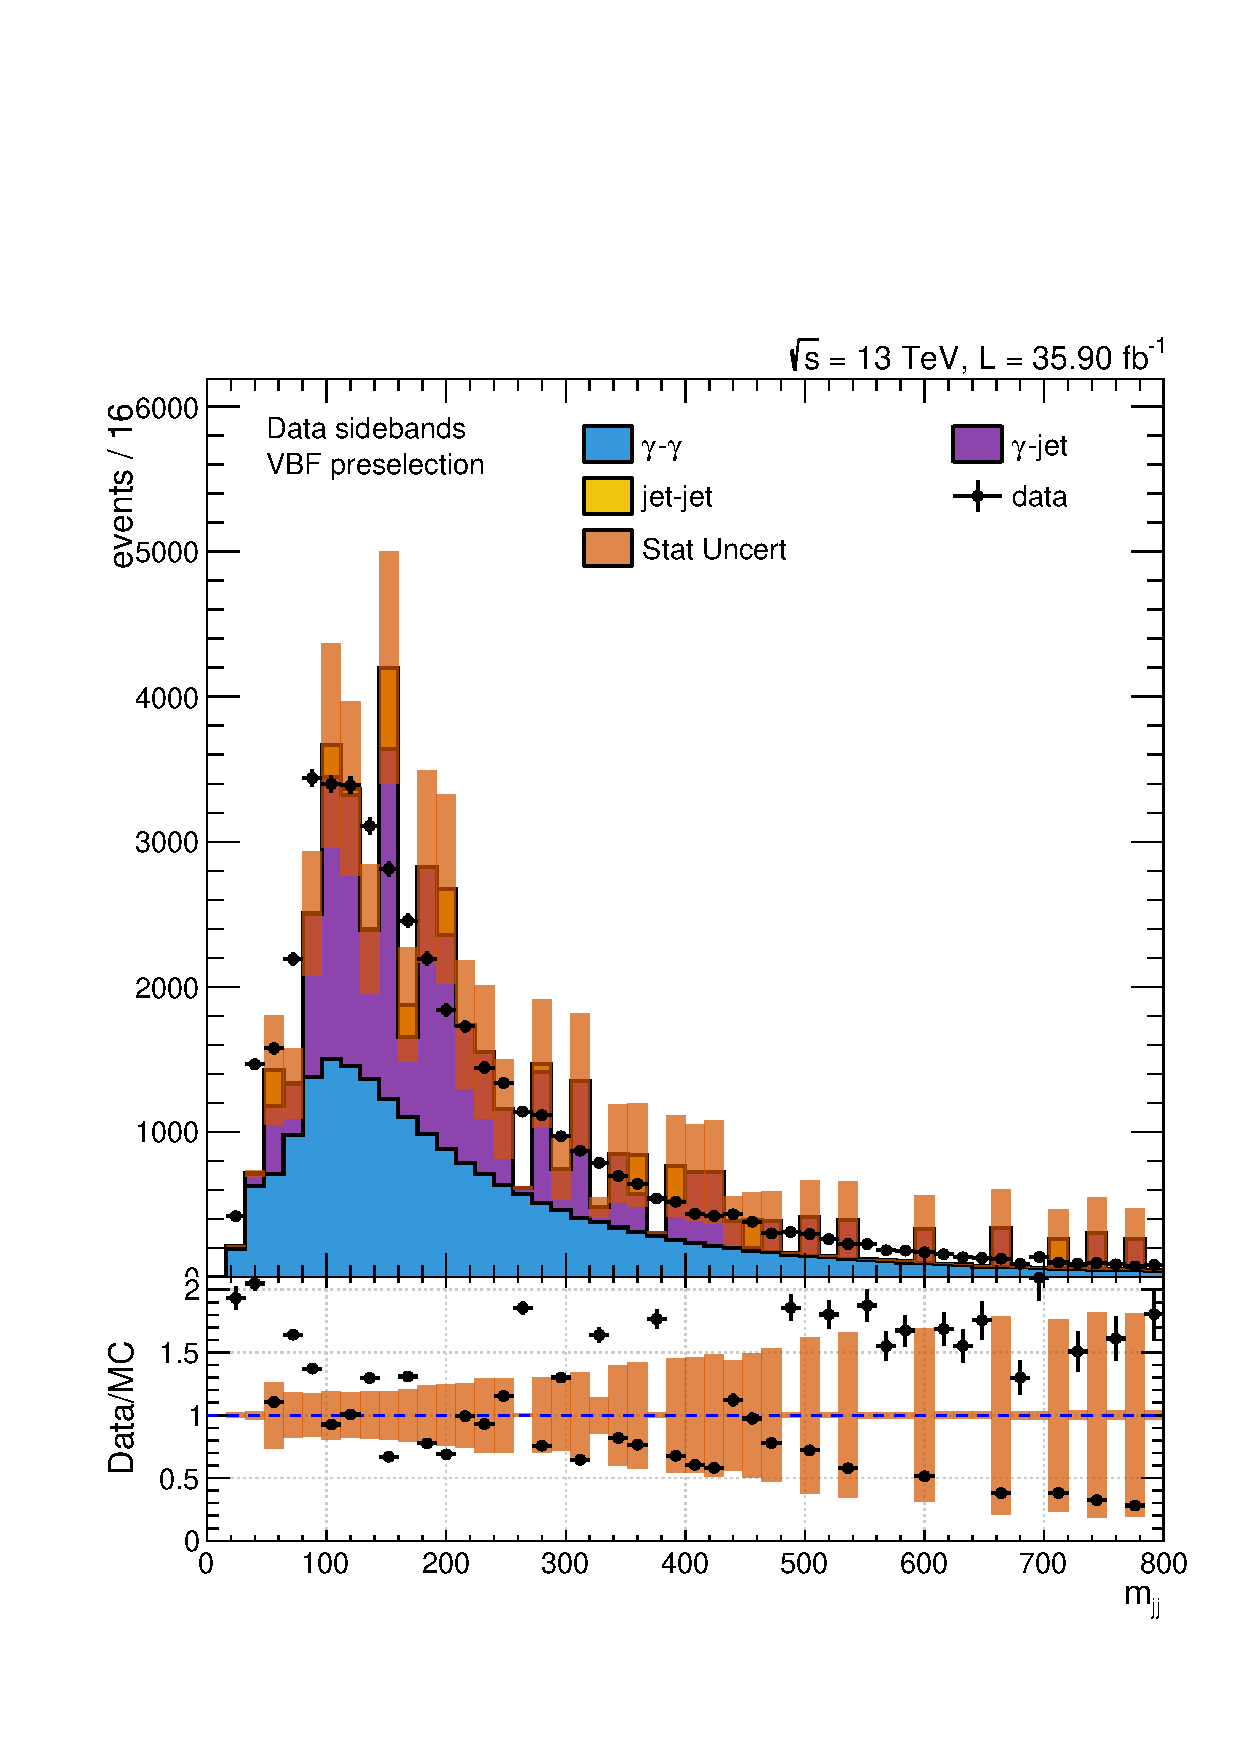
\includegraphics[width=0.49\textwidth]{Figures/Categorisation/mjj_2016.pdf}
  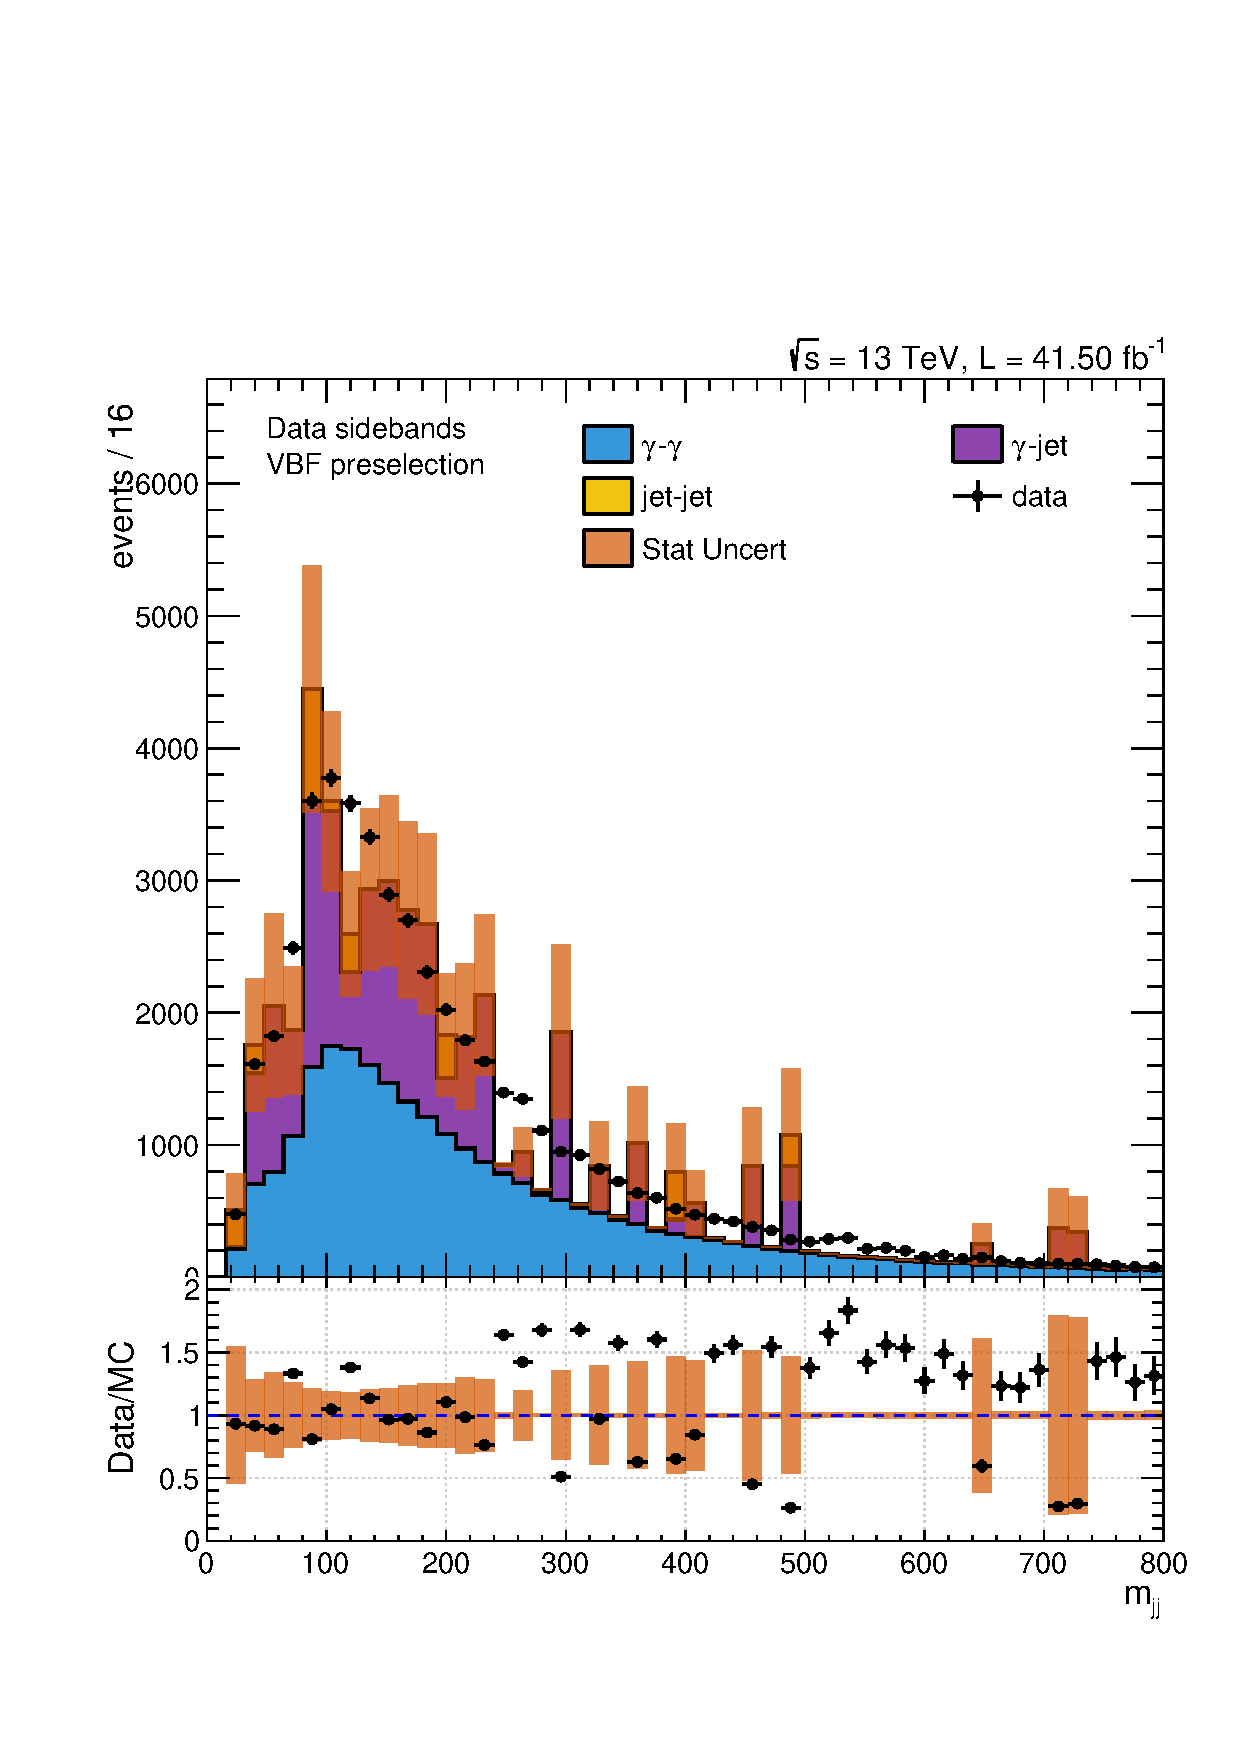
\includegraphics[width=0.49\textwidth]{Figures/Categorisation/mjj_2017.pdf}
  \caption[Dijet invariant mass distributions.]
  {
    Distribution of the dijet invariant mass in background (stacked histogram) 
    and data (black points) events.
    The statistical uncertainty is shown by the orange band.
    The left plot shows 2016 data and MC,
    with 2017 data and MC on the right.
  }
  \label{fig:cat_mjjinput}
\end{figure}

An alternative solution to this problem is to use events from a data control region 
to replace the MC samples with low numbers of events.
In this way, the more abundant data events are used to replace the simulated prompt-fake and fake-fake 
events used to train the dijet BDT.
There are a sufficient number of prompt-prompt events in MC, 
which do not need replacement and continue to be taken from simulation for the training.
This method is used for the first time in this analysis;
the outline of the procedure is as follows:
\begin{itemize}
\item define a control region by inverting the photon identification BDT requirement 
      for events entering the VBF signal region;
\item use simulation to compute the relative fraction of events in the signal region and control region, 
      for each photon, as a function of the photon kinematics;
\item apply these factors as event weights to the data in the control region 
      and use these events to replace the simulation of prompt-fake and fake-fake events in the training.
\end{itemize}

There are four distinct regions considered in the data-driven replacement method.
Events entering the analysis comprise the signal region, 
where both photons pass the photon identification BDT requirements;
the total number of events is $N_{pp}$.
There are two control regions, where one photon passes the requirement and one fails it.
The number of events in each are denoted by $N_{pf}$ 
(where the leading photon passes and the subleading photon fails) and $N_{fp}$ 
(where the leading photon fails and the subleading photon passes).
Lastly there is the region where both photons fail the requirement, with $N_{ff}$ events.
%Table~\ref{tab:cat_RegionDefinitions} shows the definition of each region.
%TODO put in table. Mention reason for gap in ID BDT score?
Figure~\ref{fig:cat_DDschematic} illustrates how the method works.

\begin{figure}
  \centering
  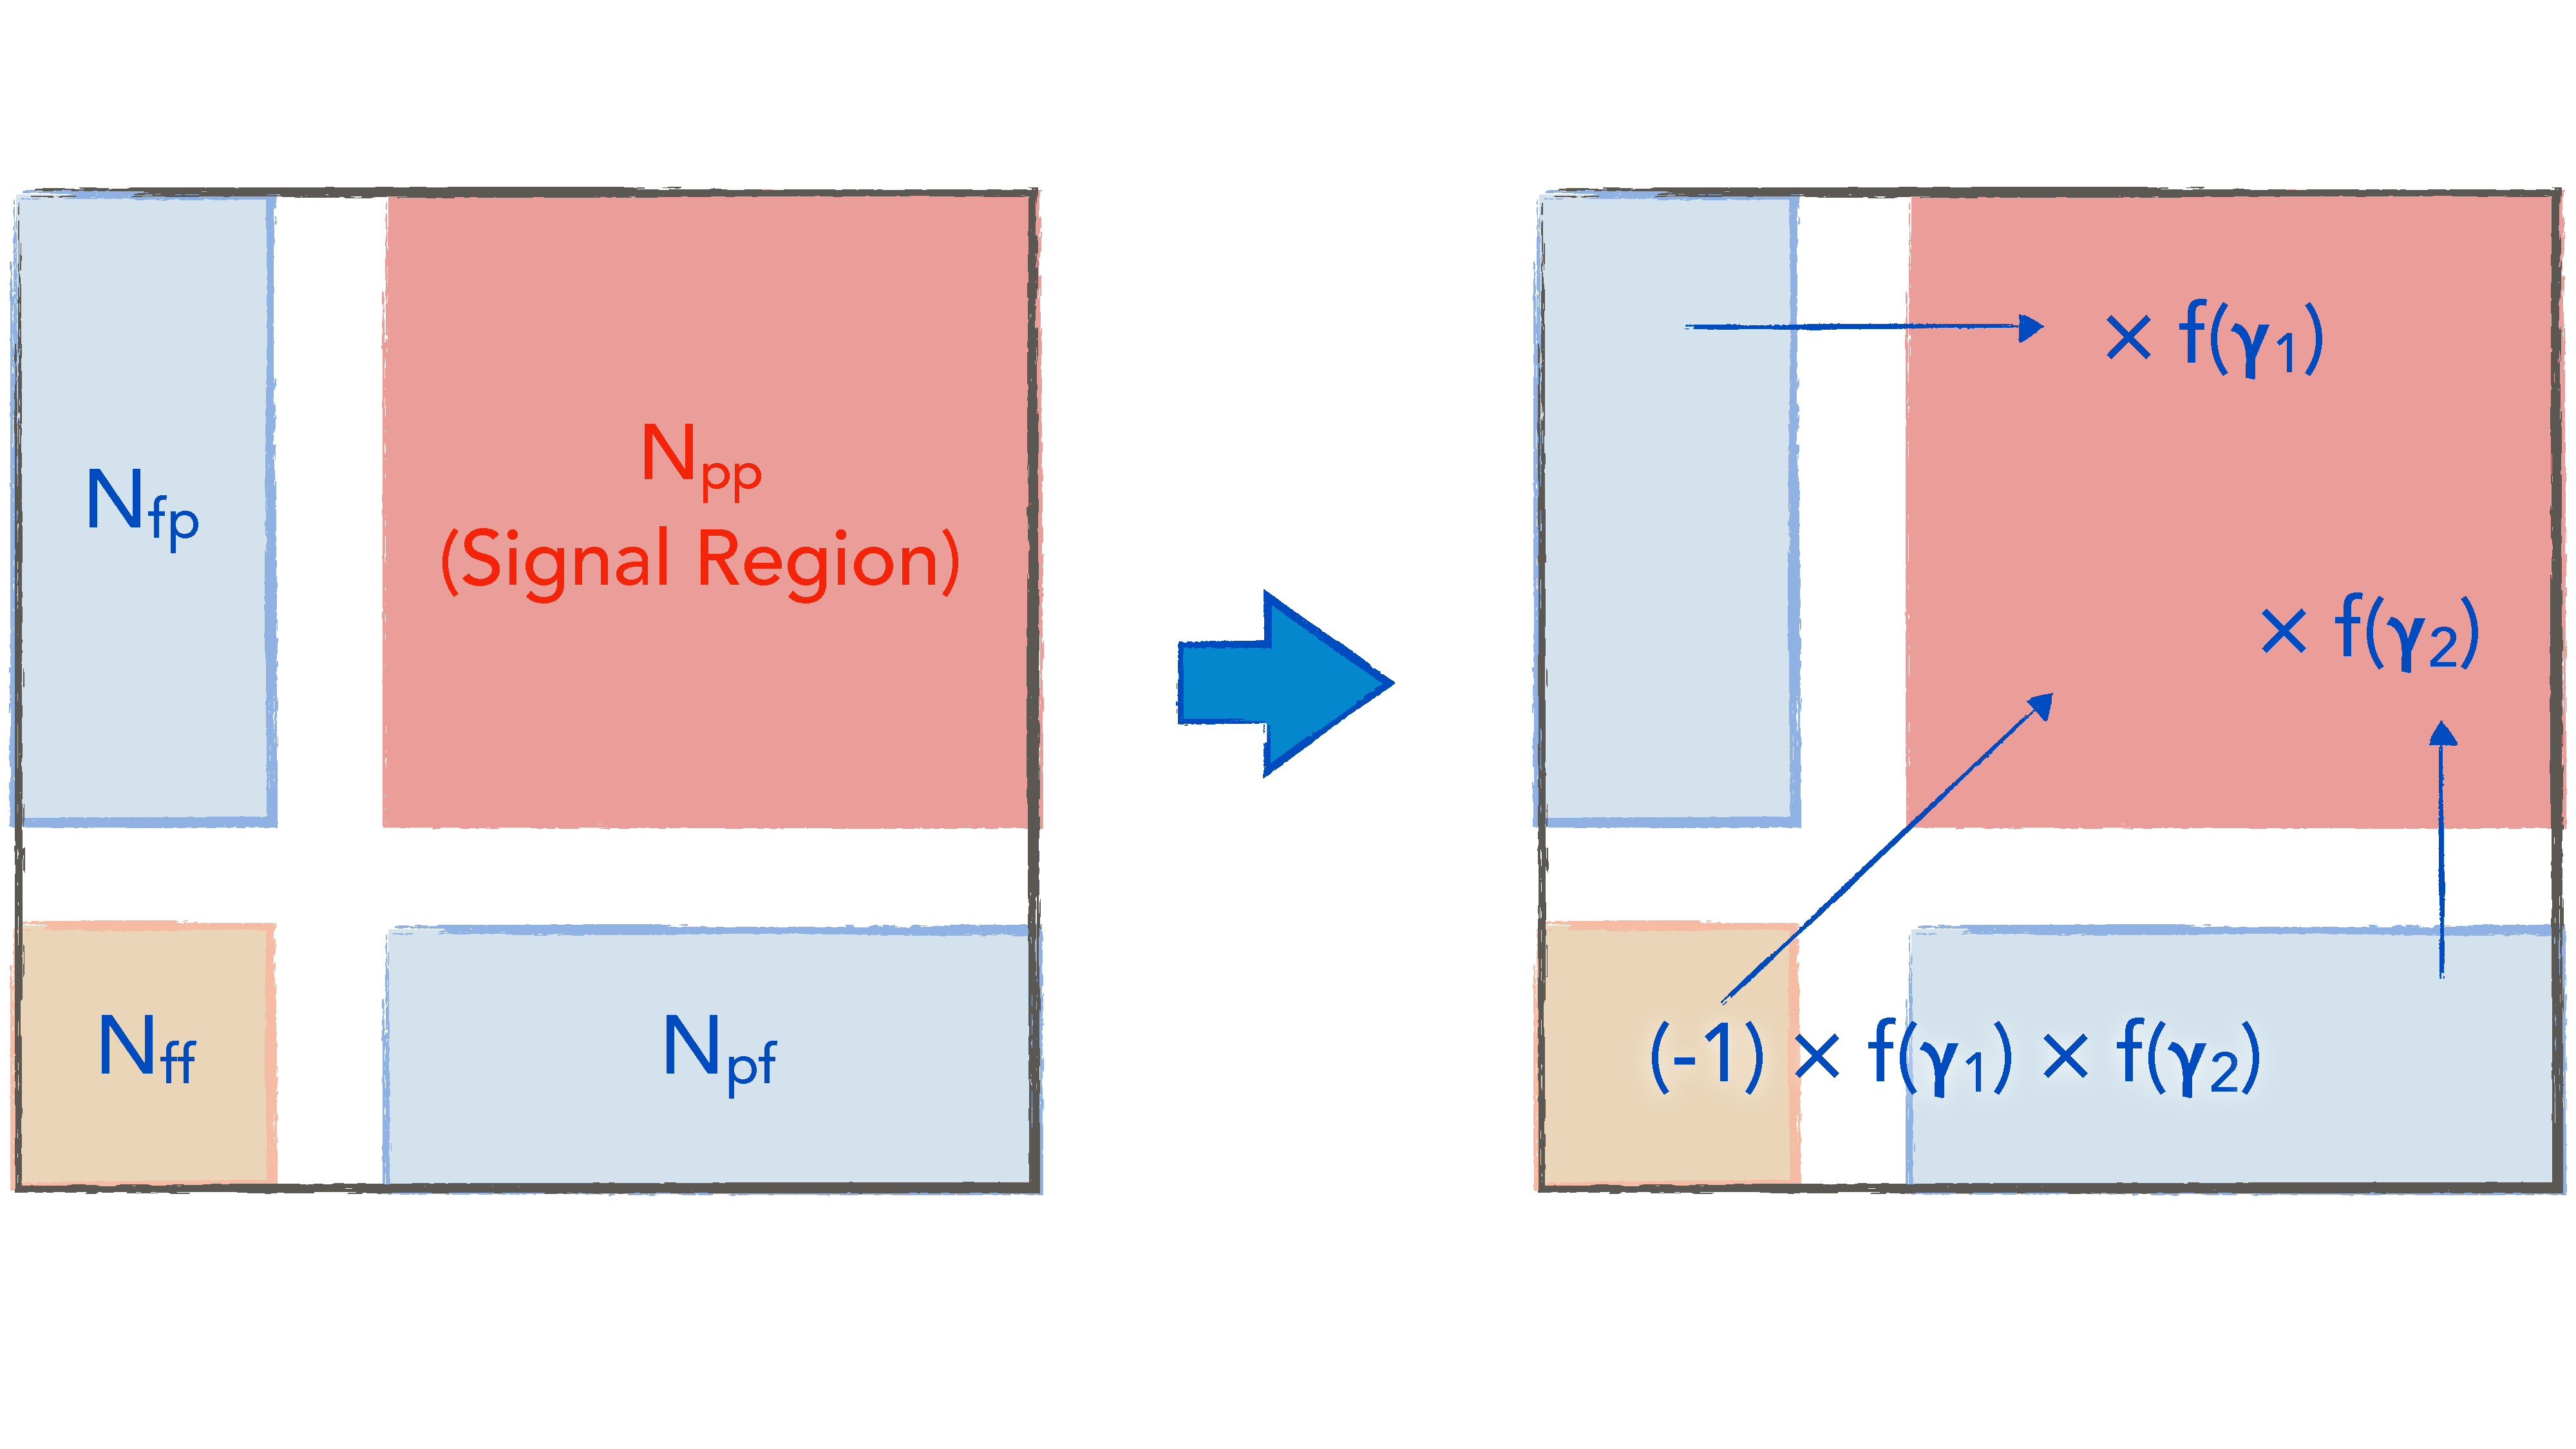
\includegraphics[width=\textwidth]{Figures/Categorisation/DDschematic.pdf}
  \caption[The data-driven method for dijet BDT training.]
  {
    A schematic illustrating the data-driven method for replacing the simulated
    prompt-fake and fake-fake events with reweighted data events from control regions 
    defined by the photon identification BDT. 
  }
  \label{fig:cat_DDschematic}
\end{figure}

Once these regions have been defined, it is possible to define so-called ``fake-factors" 
to extrapolate from the number of events in the control regions 
to the expected number of events in the signal region.
These factors are calculated from simulation, in bins of \pt and $\eta$.
Kinematic variables other than \pt and $\eta$ are assumed to be similar 
across the control and signal regions.
In order to minimise the statistical error on the fake factors, 
the loosened VBF preselection is used.
The full VBF preselection is then applied before training, 
once the events have been weighted by the fake factors.

The expression for the fake factor consists of the factor 
which extrapolates from the control region to the signal region, $w_{\textrm{fake}}$, 
multiplied by the fraction of events in the data which are either prompt-fake or fake-fake, 
$w_{\textrm{QCD}}$.
The second term is required since we wish to extract 
only the prompt-fake and fake-fake components from the data;
the prompt-prompt component is still taken from simulation.
Each term is applied to the photon which fails the identification requirement, 
and depends on the \pt and $\eta$ of this photon.
This can be written as:

\begin{equation*}
w_{\textrm{fake}} = w_{\textrm{fake}}(\eta,\pt)
= \left( \frac{N^{SR}} {N^{CR}} \right)_{MC} , 
\end{equation*}
\begin{equation*}
w_{\textrm{QCD}} = w_{\textrm{QCD}}(\eta,\pt)
= \left( \frac{N^{CR}_{pf} + N^{CR}_{ff}} {N^{CR}_{pp} + N^{CR}_{pf} + N^{CR}_{ff}} \right)_{MC} ,
\end{equation*}
\begin{equation*}
f = f(\eta,\pt) = w_{\textrm{fake}} \times w_{\textrm{QCD}} , 
\end{equation*}

where $N^{SR}$ and $N^{CR}$ are the number of events in the signal and control regions respectively;
each is a function of the photon \pt and $\eta$.
The number of prompt-prompt, prompt-fake, and fake-fake events in the control regions 
are also a function of photon \pt and $\eta$, 
and are denoted by $N^{CR}_{pp}$, $N^{CR}_{pf}$, and $N^{CR}_{ff}$ respectively.
The fake factors are calculated in four bins of \pt and two bins of $\eta$.
Figure~\ref{fig:cat_FakeFactors} shows the values of the factors in each of these bins.

\begin{figure}
  \centering
  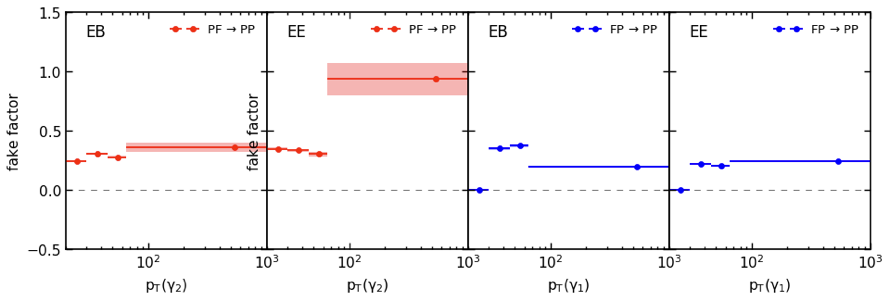
\includegraphics[width=\textwidth]{Figures/Categorisation/fakeFactors.png}
  \caption[Values of the fake factors used in the data-driven dijet BDT method.]
  {
    Fake factor values in each of the four \pt and two $\eta$ bins.
  }
  \label{fig:cat_FakeFactors}
\end{figure}

%TODO include this??
%The final expression for calculating the number of events from the data-driven method 
%also takes into account the double-counting of the $N_{ff}$ contribution.

Validation of the data-driven method is performed to confirm that its output is 
a suitable replacement for the simulation.
The new training inputs, 
comprising the simulated prompt-prompt events and data-driven prompt-fake and fake-fake events, 
are compared with data from sidebands in the diphoton mass distribution.
The usual signal region selection is applied to the sideband data, 
but with the requirement that the diphoton mass does not lie in the region $115 < \mgg < \SI{135}{GeV}$.
These data cannot be used for training the dijet BDT since its reuse in the final fits 
could then induce bias; 
however it is very useful for validating the method, 
since its kinematic properties should be essentially identical to the data-driven output.
Figure~\ref{fig:cat_DDvalidation} shows the good agreement between the data-driven output
and the sideband data. 
The figure also shows how the method solves the problem of the high-weight events present in the MC; 
this confirms that it fulfils its purpose.

\begin{figure}
  \centering
  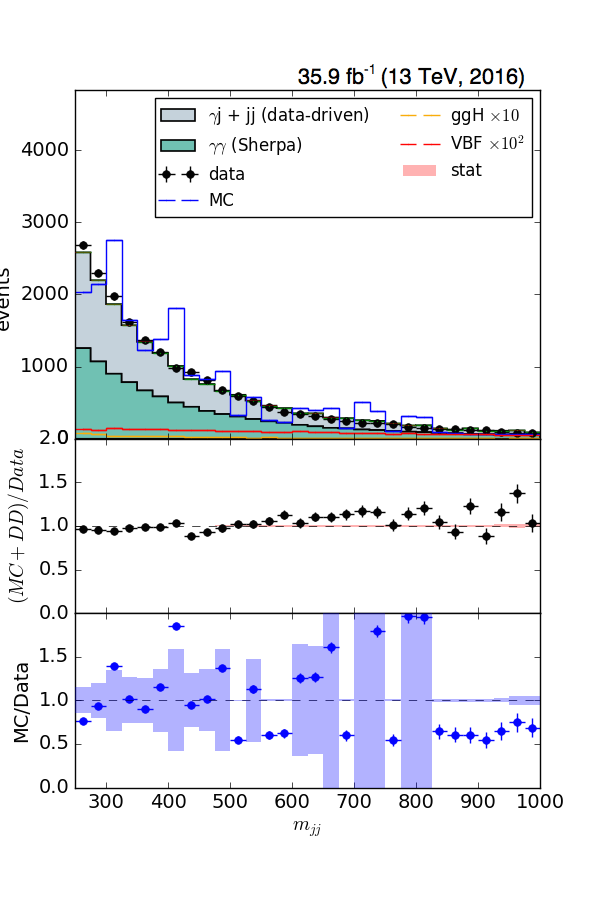
\includegraphics[width=0.49\textwidth]{Figures/Categorisation/DDvalidation_mjj2016.png}
  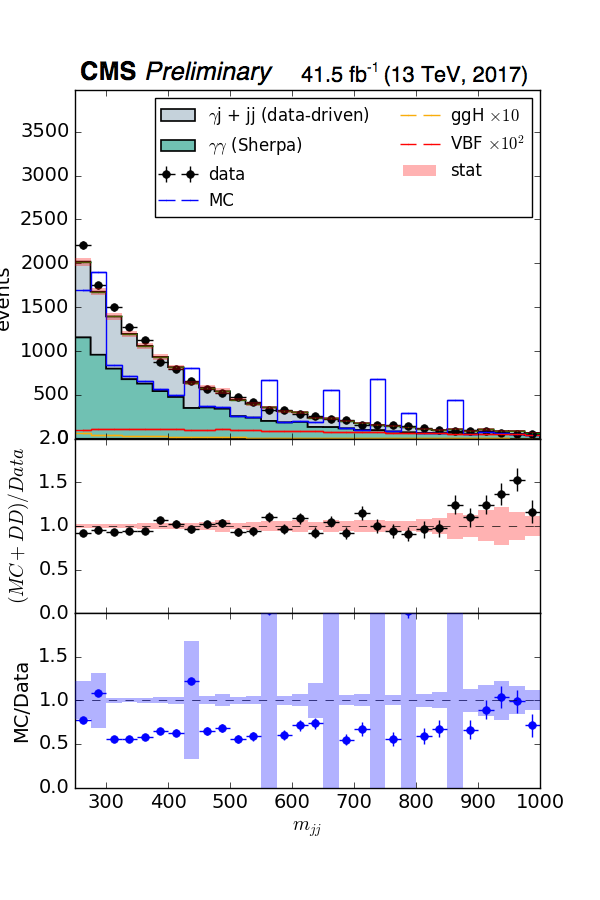
\includegraphics[width=0.49\textwidth]{Figures/Categorisation/DDvalidation_mjj2017.png}
  \caption[Validation of the data-driven method.]
  {
    Validation of the data-driven method. 
    The upper parts of the plots show the simulated background (blue histogram), 
    the background obtained with simulation for the prompt-prompt component 
    and utilising the data-driven method for the prompt-prompt and prompt-fake components 
    (green and grey stacked histograms),
    and mass sideband data (black points).
    The distributions of the ggH (yellow line) and VBF (red line) are also shown.
    Two ratio plots are also included, with one comparing the data-driven method to the sideband data, 
    and the other comparing the simulation with the sideband data.
    Data and simulation from 2016 are shown on the left, with 2017 on the right.
  }
  \label{fig:cat_DDvalidation}
\end{figure}

The dijet BDT is then trained with the data-driven inputs.
For the 2016 dataset, the area under the ROC curve is 0.87.
This constitutes a significant improvement over the score when the BDT is trained only with simulation, 
which is 0.84.
As an additional cross-check, the BDT is trained with events from the data sideband. 
The area of this ROC curve is also 0.87, 
which confirms that the observed improvement is reasonable.
The performance is 2017 is very similar, 
with the data-driven method improving in the ROC score from 0.83 to 0.86.

The agreement between data and simulation for the dijet BDT score is validated 
in a similar way to the diphoton BDT.
Events from the \Zee control region are required to pass the VBF preselection.
Figure~\ref{fig:cat_dijetBDT} shows the output score of the dijet BDT for data and simulation.
The systematic uncertainties included in the plot are those affecting the 
jet energy scale and the jet energy resolution corrections.
Good agreement is observed between the data and simulation in both years, 
with all discrepancies covered by the statistical and systematic uncertainties.

\begin{figure}[hptb]
  \centering
  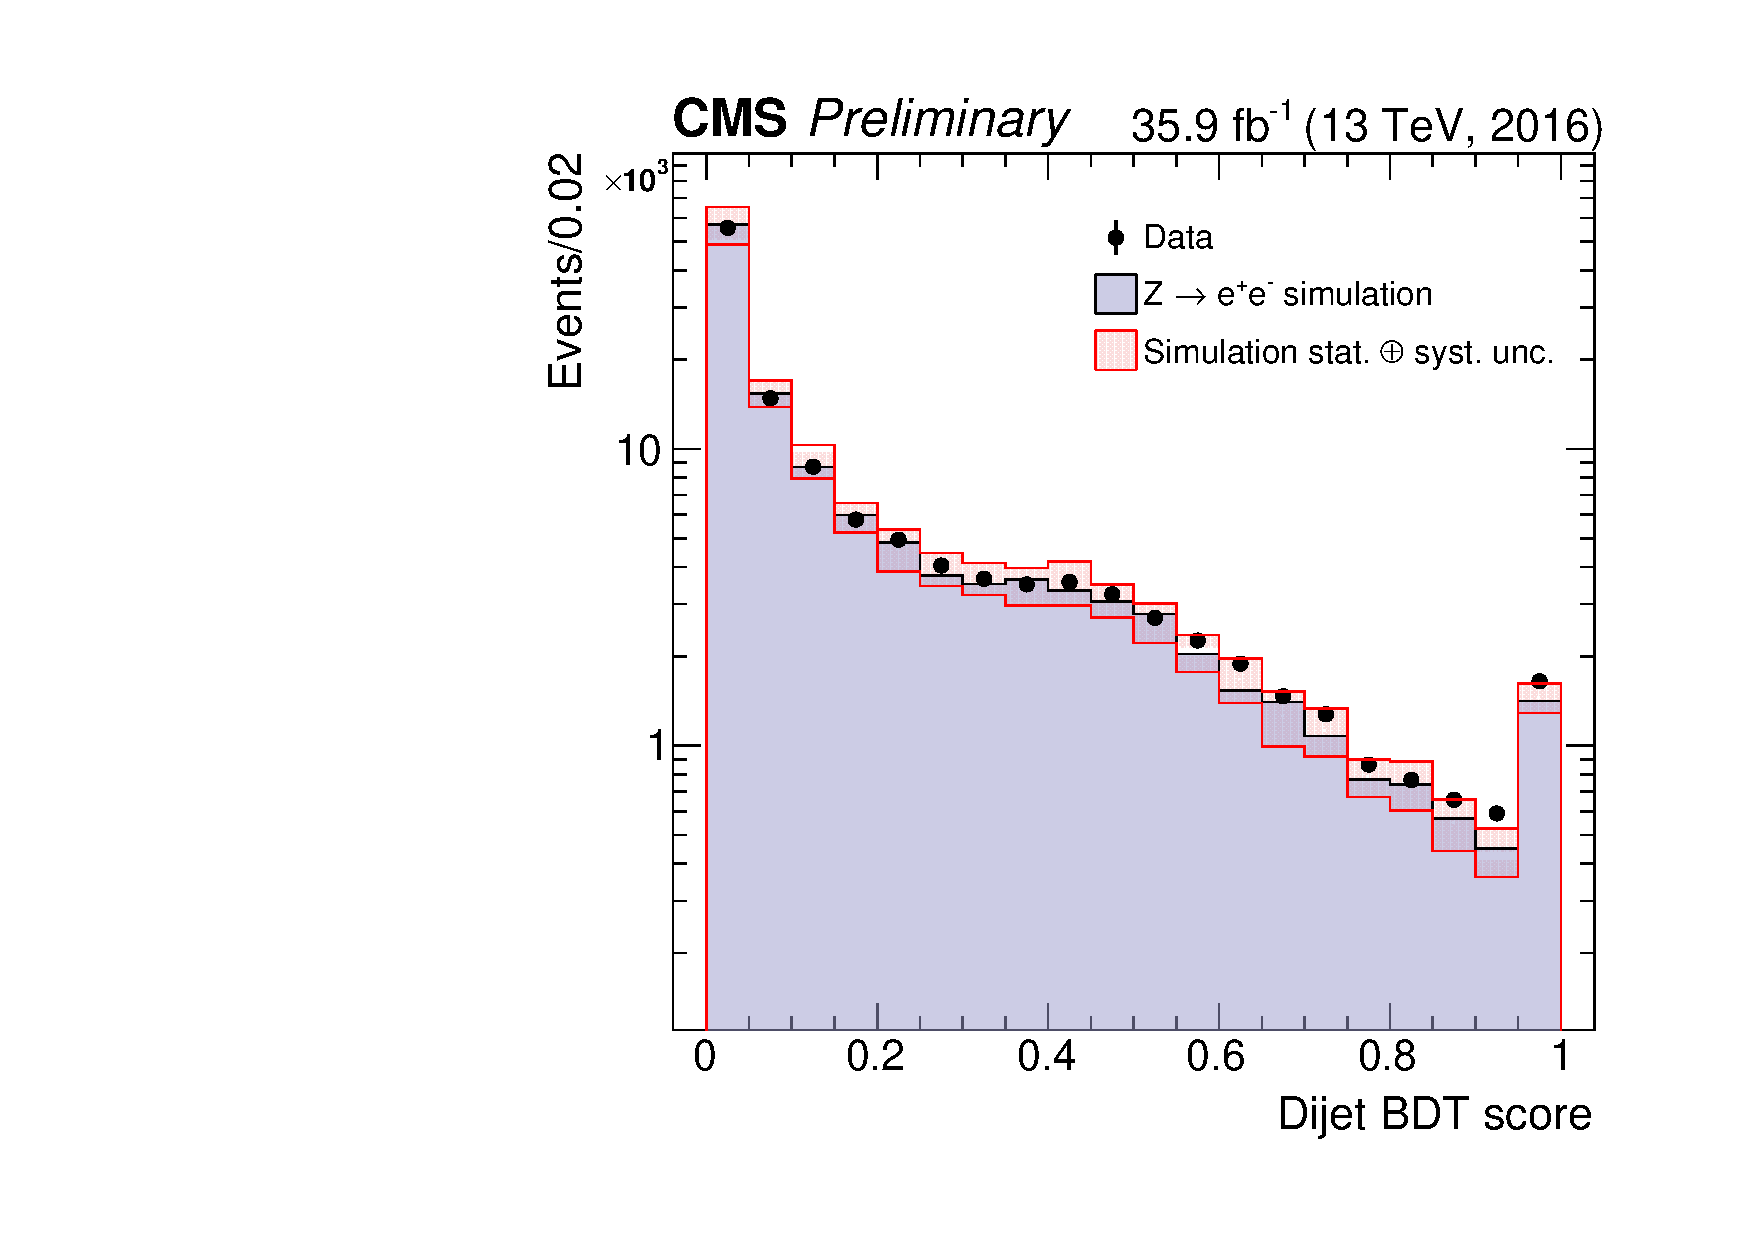
\includegraphics[width=0.7\textwidth]{Figures/Categorisation/DijetBDT_2016.pdf}
  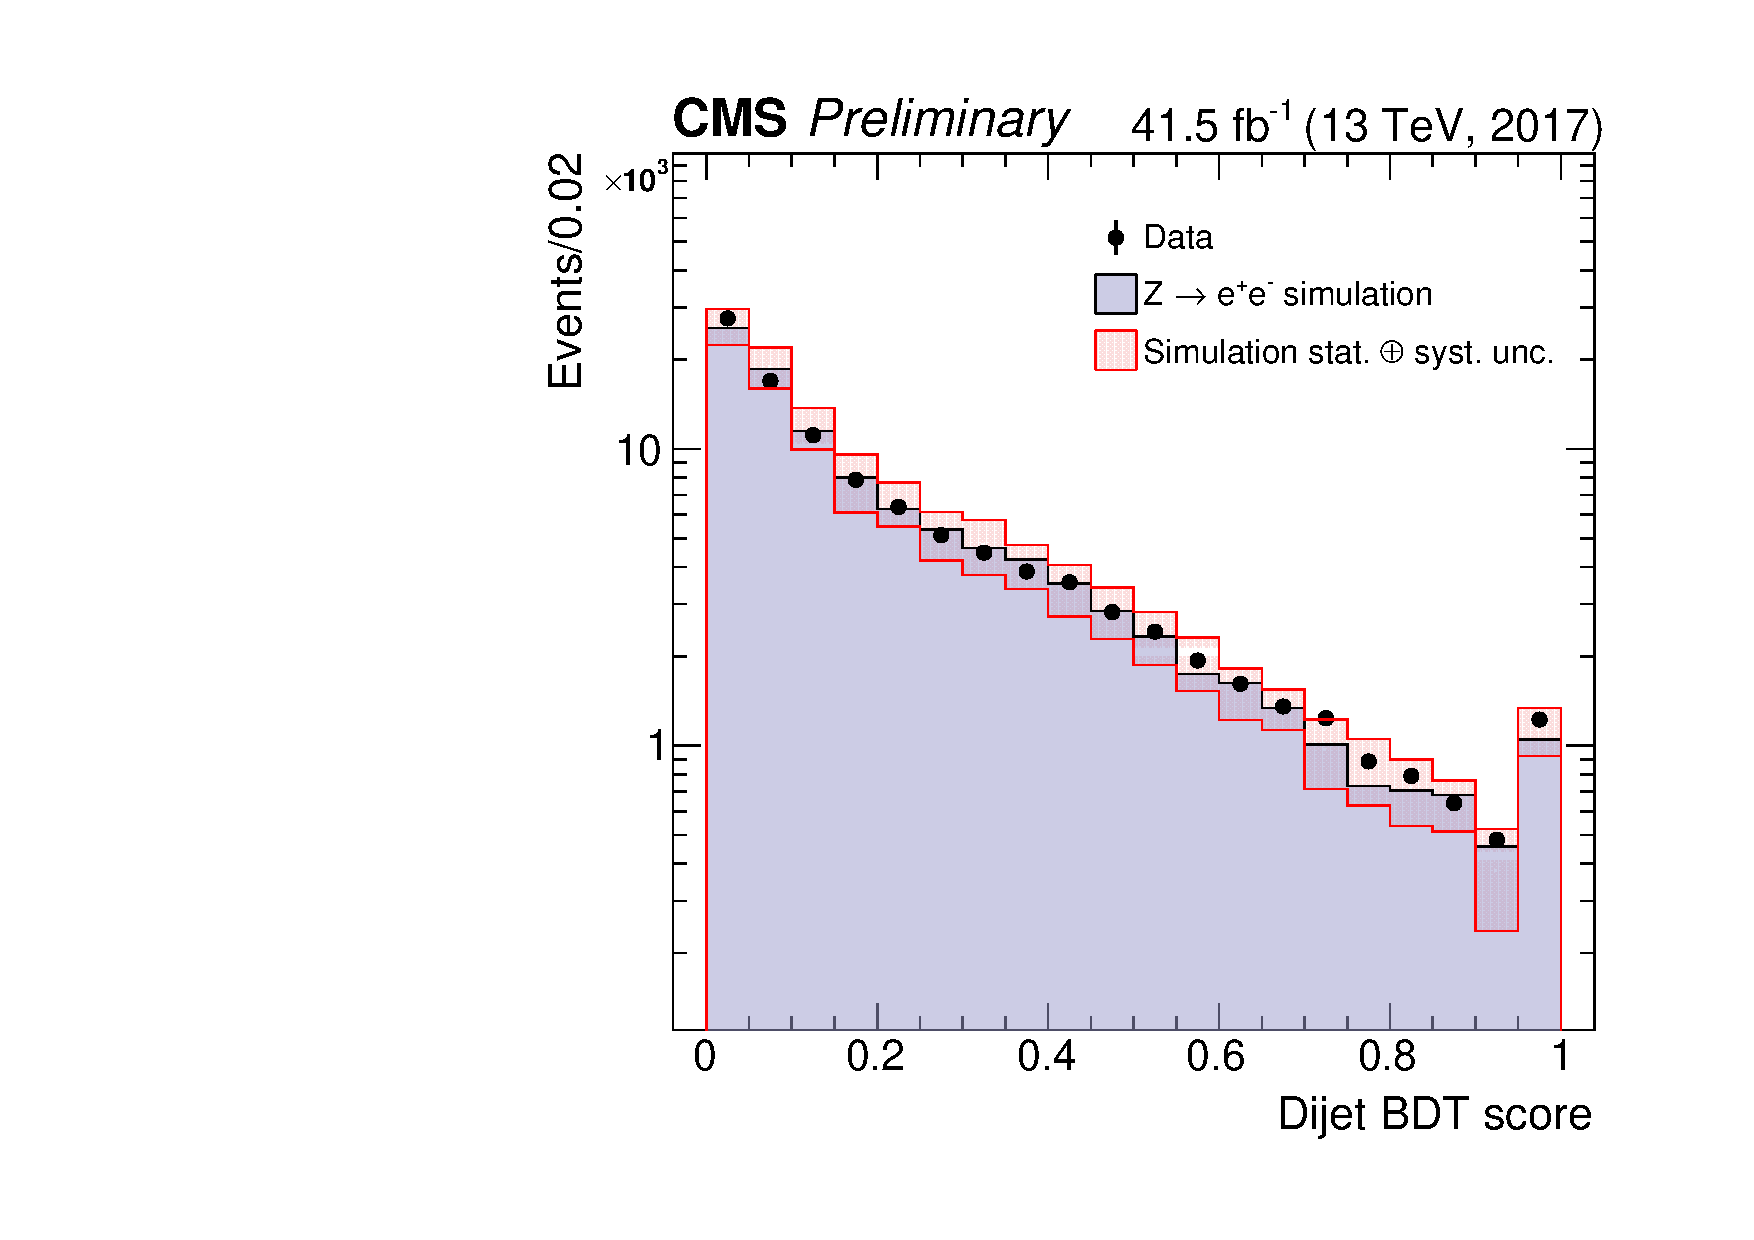
\includegraphics[width=0.7\textwidth]{Figures/Categorisation/DijetBDT_2017.pdf}
  \caption[Validation of the dijet BDT in \Zee events.]
  {
    Score of the dijet BDT in $\Zee$
    events where the electrons are reconstructed as photons.
    The points show the score for data, the histogram shows
    the score for simulated Drell--Yan events, including statistical and 
    systematic uncertainties (pink band).
    The top plot shows 2016 data and MC,
    with 2017 data and MC on the bottom.
    Figures first shown in Ref.~\cite{HIG-18-029}.
  }
  \label{fig:cat_dijetBDT}
\end{figure}

\subsection{Category definitions}

In previous versions of the analysis, 
the categories targeting VBF production were defined using the so-called ``combined BDT".
The combined BDT is designed to incorporate both the dijet and diphoton information 
in order to optimally construct the VBF categories.
Its input variables are:
\begin{itemize}
\item the diphoton BDT score
\item the dijet BDT score
\item the transverse momentum of the two leading photons, divided by the diphoton mass, $\pt^{1,2}/\mgg$;
\end{itemize}
The combined BDT is trained with VBF as signal against the three sources of SM background, 
using simulated events in each case.
Gluon fusion is not included in the training because it is found to worsen the performance 
of the combined BDT to reject true background.
Since these backgrounds have a greater impact on the final sensitivity 
than the contamination from other signal processes, 
this is considered a higher priority.
However, it does mean that the ggH rejection of the combined BDT can be sub-optimal.
Here the efficacy of the combined BDT is compared with the more direct approach of 
defining the VBF categories by imposing thresholds on the diphoton and dijet BDT scores directly.

In addition to comparing the two different BDT approaches, 
different possible categorisation scenarios are considered.
In Ref.~\cite{HIG-16-040}, three inclusive categories are defined 
by placing thresholds on the output score of the combined BDT.
For this analysis, further splitting using kinematic variables is required 
if the different VBF stage 1 bins are to be measured individually.
%However it is found that optimising for each stage 1 bin independently, 
%considering only one stage 1 bin as signal in each case, 
%reduces the overall sensitivity to the VBF process.
%Therefore when comparing different categorisation scenarios,
When comparing different categorisation scenarios,
the figure of merit considered is the total VBF significance, 
computed using the AMS metric with all VBF bins considered as signal.
Scenarios with additional splits following the stage 1 bin definitions 
will then be considered preferable, 
provided they do not substantially reduce the overall VBF significance, 
since they enable individual stage 1 bins to be measured in addition to the overall VBF cross section.
In each scenario, there is a single dedicated VBF BSM category 
which requires that the \pt of the leading jet is greater than \SI{200}{GeV}.
The list of scenarios considered is as follows:
\begin{itemize}
\item \textbf{Inclusive two category:} Two categories are considered, 
      with no additional kinematic selection criteria applied.
      Including the VBF BSM category, this gives three categories in total.
\item \textbf{Inclusive three category:} Three categories are considered, 
      with no additional kinematic selection criteria applied.
      It is almost equivalent to the approach in Ref.~\cite{HIG-16-040}, 
      aside from the additional VBF BSM category.
      This gives a total of four categories.
\item \textbf{Split by \ptHjj:} Two categories are considered 
      for each of the 2J-like and 3J-like VBF bins,
      using a boundary at \SI{25}{GeV} on the reconstructed value of \ptHjj.
      This gives a total of five categories.
\item \textbf{Split by \ptHjj and \mjj:} Two categories are considered
      for each of the 2J-like and 3J-like VBF bins,
      using a boundary at \SI{25}{GeV} on the reconstructed value of \ptHjj.
      Additionally, the requirement that \mjj is greater than \SI{400}{GeV} is applied.
      A fifth category targeting principally the ``VBF rest" bin, with $250 < \mjj < 400$,
      is therefore included.
      This gives a total of six categories.
\end{itemize}

A boundary optimisation procedure is followed for each scenario, 
using the same methodology as for the ggH categories.
For the approach which uses the diphoton and dijet BDT output scores directly, 
the values of the thresholds on the two BDTs are optimised simultaneously for each category.
The resulting significance values of each scenario for the 2016 and 2017 datasets 
are shown in Tables~\ref{tab:cat_VBFscenarios2016} and \ref{tab:cat_VBFscenarios2017} respectively.
The performance of the combined BDT approach is compared with the approach using the diphoton 
and dijet BDT scores directly in each case.
For both years, the combined BDT performs slightly worse 
than the direct use of the diphoton and dijet BDTs.
This can be attributed to the fact that the combined BDT is trained only on simulation; 
it is not possible to use the data-driven method for its training 
since the photon information is used as inputs.
Furthermore, the results demonstrate that there is no substantial reduction 
in the overall VBF significance with the most granular categorisation scenario.
It is therefore considered the best scenario for facilitating measurements of individual stage 1 bins, 
and is chosen as the VBF categorisation scheme for the analysis.

Tables~\ref{tab:cat_VBFcuts2016} and \ref{tab:cat_VBFcuts2017} show the final thresholds 
for the diphoton and dijet BDTs in each category, 
together with the expected number of signal and background events and the per-category significance.

\begin{table}
  \begin{centering}
    \begin{tabular}{ r | c | c }
\hline
Scenario                          & Dijet + Diphoton BDT    & Combined BDT   \\
\hline
Inclusive 2 category              & 2.43$\sigma$            & 2.26$\sigma$   \\
Inclusive 3 category              & 2.55$\sigma$            & 2.31$\sigma$   \\
Split by $p_T^{Hjj}$              & 2.38$\sigma$            & 2.28$\sigma$   \\
Split by $p_T^{Hjj}$ and $m_{jj}$ & 2.53$\sigma$            & 2.43$\sigma$   \\
\hline
\end{tabular}

    \caption[Comparison of 2016 VBF categorisation scenarios.]
    {
      The total VBF significance (defined by the AMS metric) for different categorisation scenarios 
      using 2016 data and simulation, assuming an integrated luminosity of \SI{35.9}{\fbinv}.
      Classification using the combined BDT is compared with setting boundaries with the 
      diphoton and dijet BDTs directly.
    }
    \label{tab:cat_VBFscenarios2016}
  \end{centering}
\end{table}

\begin{table}
  \begin{centering}
    \begin{tabular}{ r | c | c }
\hline
Scenario                          & Dijet + Diphoton BDT    & Combined BDT   \\
\hline
Inclusive 2 category              & 2.70$\sigma$            & 2.52$\sigma$   \\
Inclusive 3 category              & 2.73$\sigma$            & 2.61$\sigma$   \\
Split by $p_T^{Hjj}$              & 2.68$\sigma$            & 2.54$\sigma$   \\
Split by $p_T^{Hjj}$ and $m_{jj}$ & 2.73$\sigma$            & 2.60$\sigma$   \\
\hline
\end{tabular}

    \caption[Comparison of 2017 VBF categorisation scenarios.]
    {
      The total VBF significance (defined by the AMS metric) for different categorisation scenarios 
      using 2017 data and simulation, assuming an integrated luminosity of \SI{41.5}{\fbinv}.
      Classification using the combined BDT is compared with setting boundaries with the 
      diphoton and dijet BDTs directly.
    }
    \label{tab:cat_VBFscenarios2017}
  \end{centering}
\end{table}

\begin{table}
  \begin{centering}
    \begin{tabular}{ r | c | c | c | c | c } 
\hline 
Category       & Dijet BDT cut & Diphoton BDT cut & Signal & Background & Significance \\ 
\hline 
2J-like  Tag 0 & 0.12         & 0.62             & 8.2    & 7.0        & 2.04         \\
2J-like  Tag 1 & -0.89        & 0.72             & 3.1    & 14.9       & 0.68         \\
3J-like  Tag 0 & 0.48         & 0.61             & 4.7    & 8.8        & 1.07         \\
3J-like  Tag 1 & -0.84        & 0.74             & 3.2    & 35.7       & 0.46         \\
VBF BSM  Tag   & -0.41        & 0.73             & 2.2    & 7.7        & 0.53         \\
VBF Rest Tag   & -0.74        & 0.77             & 2.5    & 34.3       & 0.36         \\
\hline 
\end{tabular}

    \caption[Definitions of 2016 categories targeting VBF production.]
    {
      The chosen diphoton and dijet BDT boundaries, 
      the expected number of signal (S) and background (B) events, 
      and the expected significance (defined by the AMS metric) of each category in the VBF phase space 
      for 2016 data and simulation, assuming an integrated luminosity of \SI{35.9}{\fbinv}.
    }
    \label{tab:cat_VBFcuts2016}
  \end{centering}
\end{table}

\begin{table}
  \begin{centering}
    \begin{tabular}{ r | c | c | c | c | c } 
\hline 
Category       & Dijet BDT cut & Diphoton BDT cut & S & B & AMS \\ 
\hline 
2J-like  Tag 0 & -0.39        & 0.75            & 7.5    & 9.2        & 1.73         \\
2J-like  Tag 1 & -0.89        & 0.68            & 1.5    & 14.5       & 0.33         \\
3J-like  Tag 0 & 0.03         & 0.77            & 4.7    & 12.0       & 1.00         \\
3J-like  Tag 1 & -0.69        & 0.57            & 2.1    & 36.9       & 0.31         \\
VBF BSM Tag    & -0.27        & 0.78            & 2.3    & 6.3        & 0.59         \\
VBF Rest Tag   & -0.62        & 0.73            & 2.8    & 38.0       & 0.38         \\
\hline 
\end{tabular}

    \caption[Definitions of 2017 categories targeting VBF production.]
    {
      The chosen diphoton and dijet BDT boundaries, 
      the expected number of signal (S) and background (B) events, 
      and the expected significance (defined by the AMS metric) of each category in the VBF phase space 
      for 2017 data and simulation, assuming an integrated luminosity of \SI{41.5}{\fbinv}.
    }
    \label{tab:cat_VBFcuts2017}
  \end{centering}
\end{table}

\section{Summary}

A set of \Hgg analysis categories are defined in order to maximise the overall sensitivity 
of the analysis and to enable the measurement of different signal bins.
Categories targeting nine different subdivisions of the ggH production mode are constructed, 
using the reconstructed \ptgg and number of jets to infer the most likely signal bin.
The diphoton BDT is then used to further split these events into categories of differing S/B, 
which increases the precision of the measurement of each bin.
Furthermore, categories targeting the different VBF signal bins are constructed.
A dijet BDT is trained using a novel data-driven approach, 
and is used to discriminate against both ggH production and background processes.
It is used together with the diphoton BDT and the reconstructed values of \mjj, \ptHjj 
and the number of jets to define the final VBF analysis categories.

\chapter{Statistical Methodology}
\label{chap:stats}

Statistical methodology chapter goes here.

\chapter{Results}
\label{chap:results}

\section{Introduction}

The principal aim of this analysis is to measure Higgs boson simplified template cross sections, 
at both stage 0 and stage 1, and their associated uncertainties.
This is achieved by performing a simultaneous fit of the signal and background models 
to the observed \mgg distribution in each category.
A binned maximum likelihood fit is performed in the range $100 < \mgg < \SI{180}{GeV}$, 
with a bin size of \SI{250}{MeV};
this is sufficiently small relative to the diphoton mass resolution 
that a negligible amount of information is lost. %and is computationally much faster

The likelihood function in each category, $\Like_c$, is expressed as:
\begin{equation}
\Like_c(\Largs) = \prod^{N_b}_{i=1} \textrm{Poisson}\left( d_i\,|\, 
                  s_i(\vec{\sigma},\mH,\vec{\theta}) + b_i(\vec{\theta}) \right) \times C(\vec{\theta}),
\end{equation}
where $\vec{\sigma}$ is the set of parameters of interest (POIs), 
which in this analysis are always a set of one or more cross section parameters;
$\vec{\theta}$ is the set of nuisance parameters which affect the measurements 
but are not themselves of interest;
$N_b$ is the number of bins used in the category's \mgg distribution;
Poisson indicates a Poisson function evaluated with the observed number of events 
in the $i^{\mathit{th}}$ bin $d_i$ 
and expected number of events given by the sum of the signal expectation $s_i$ 
and the background expectation $b_i$;
$C(\vec{\theta})$ is the constraint term which penalises deviations 
from the expected values of the signal nuisance parameters,
and applies a penalisation term according to 
the total number of degrees of freedom in the background model.
The expected number of signal events in each bin depends on the POIs, \mH, 
and the nuisance parameters, 
whilst the expected number of background events depends only on unconstrained nuisance parameters.

The total likelihood \Like is then given by the product of the likelihoods over all categories:
\begin{equation}
\Like(\Largs) = \prod^{N_c}_{c=1} \Like_c(\Largs),
\end{equation}
where $N_c$ is the total number of analysis categories.
The fit is then performed by minimising the value of the negative log-likelihood, \NLL, where
\begin{equation}
\NLL = -2\ln\Like(\Largs).
\end{equation}
The free parameters in the fit are the parameters of interest, \
mH, and the background nuisance parameters;
the signal nuisance parameters can vary but are constrained by the $C(\theta)$ term.
The \NLL is constructed and minimised numerically within the RooFit~\cite{RooFit} 
software package for statistical data analysis.
The values of the parameters which give the minimum value of the \NLL
are then described as the ``best-fit" values.

A frequentist approach is followed in order to extract the uncertainties on the POIs, 
in addition to their best-fit values.
The likelihood ratio test statistic, \dNLL, is constructed for a range of POI values:
\begin{equation}
\dNLL = -2\ln\frac{ \Like(\textrm{data}\,|\,\vec{\sigma},\hat{\hat{m}}_H,\vec{\hat{\hat{\theta}}}) }
                  { \Like(\textrm{data}\,|\,\vec{\hat{\sigma}},\hat{m}_H,\vec{\hat{\theta}}) },
\end{equation}
where $\hat{\hat{m}}_H$ and $\vec{\hat{\hat{\theta}}}$ are the best-fit values 
of the Higgs boson mass and nuisance parameters at the POI values $\vec{\hat{\sigma}}$;
$\vec{\hat{\sigma}}$, $\hat{m}_H$, and $\vec{\hat{\theta}}$ are the global best-fit values 
of the POIs, Higgs boson mass, and nuisance parameters respectively.
The distribution of the likelihood ratio test statistic 
can then be used to infer the approximate uncertainties on the measurements.
For a sufficient number of events, %in each bin??
the distribution tends to that of a $\chi^2$~\cite{Asymptotic}, 
where the number of degrees of freedom is equal to the number of POIs being measured.
In this case, the 68\% confidence level (CL) intervals 
are given approximately by the corresponding region for a $\chi^2$ distribution, 
which depends on the number of degrees of freedom.
For a single POI, the region is defined by $\dNLL < 1$.
The interpretation of the 68\% CL intervals within the frequentist paradigm 
is that in an ensemble of identical pseudo-experiments, 
the observed interval should should contain the true value of the POI in 68\% of cases.
The crossing points of the \dNLL at $\pm 1$ are therefore quoted
as the 68\% CL uncertainties on the POI in question.

In this analysis, the POIs considered are Higgs boson simplified template cross sections, 
which are defined at various levels of granularity and denoted by the symbol $\sigma$.
The stage 0 cross sections are equivalent 
to the sum of the individual stage 1 cross sections.
This makes clear that parameters can be defined as sums of different STXS bins, 
not just individual bins themselves.
Measuring a wider set of STXS bins provides more information, 
but the uncertainties are correspondingly larger than if fewer parameters are measured.
Therefore in this section results are reported under various scenarios, 
with between one and thirteen POIs in total.

In each case, the fit is performed with cross sections as the parameters of interest.
After each cross section has been measured, the value is normalised to the SM prediction. 
This procedure differs from that used to measure a signal strength $\mu$, 
as defined in Chapter~\ref{chap:theory},
where the parameter in the fit is the ratio of the observed cross section to the SM prediction.
The key difference between the two is that in the signal strength measurements,
the uncertainty on the SM prediction must be considered in the fit
because it enters directly in the denominator of the parameter of interest.
In contrast, the STXS measurements do not include these uncertainties on the SM yield;
the measured cross sections do not directly depend on the SM prediction.
This ensures the measurements are as independent as possible of the current SM predictions
and their uncertainties, 
which means they remain useful if theoretical advances are made in the future.

In the following section, the observed diphoton mass distribution
and the composition of the analysis categories are presented.
The remainder of chapter describes the results of stage 0 and stage 1 measurements 
within the STXS framework.
All results were first reported in Ref.~\cite{HIG-18-029}.

\section{Observed diphoton mass distributions}

The observed diphoton mass distribution is displayed together with the result 
of a signal plus background fit in Figure~\ref{fig:results_MassPlot}.
The fit contains one signal parameter, 
which includes all signal events where $|y_H| < 2.5$.
The fit is performed simultaneously to all analysis categories.
In the plot, each cateogry is summed with a weight 
corresponding to the ratio of signal events to background events. %this shows the "true" sensitvity?
The uncertainty on the background prediction is also shown.
The signal peak due to Higgs boson production is clearly visible.
%The background-only hypothesis is excluded with a significance of more than five standard deviations.

The result of the same single parameter fit is also shown in Figure~\ref{fig:results_MassPlots}.
In this case, only certain subsets of categories are included in the sum.
The \mgg distributions for the weighted sum of the categories targeting 
ggH 0J, ggH 1J, ggH 2J, and VBF production are shown.
The plots indicate the total number of events and approximate signal to background ratio
for the different processes targeted in this analysis.

The full set of unweighted diphoton mass distributions for each category 
considered in the analysis are contained in Appendix~\ref{app:massplots}.

\begin{figure}[hptb]
  \centering
  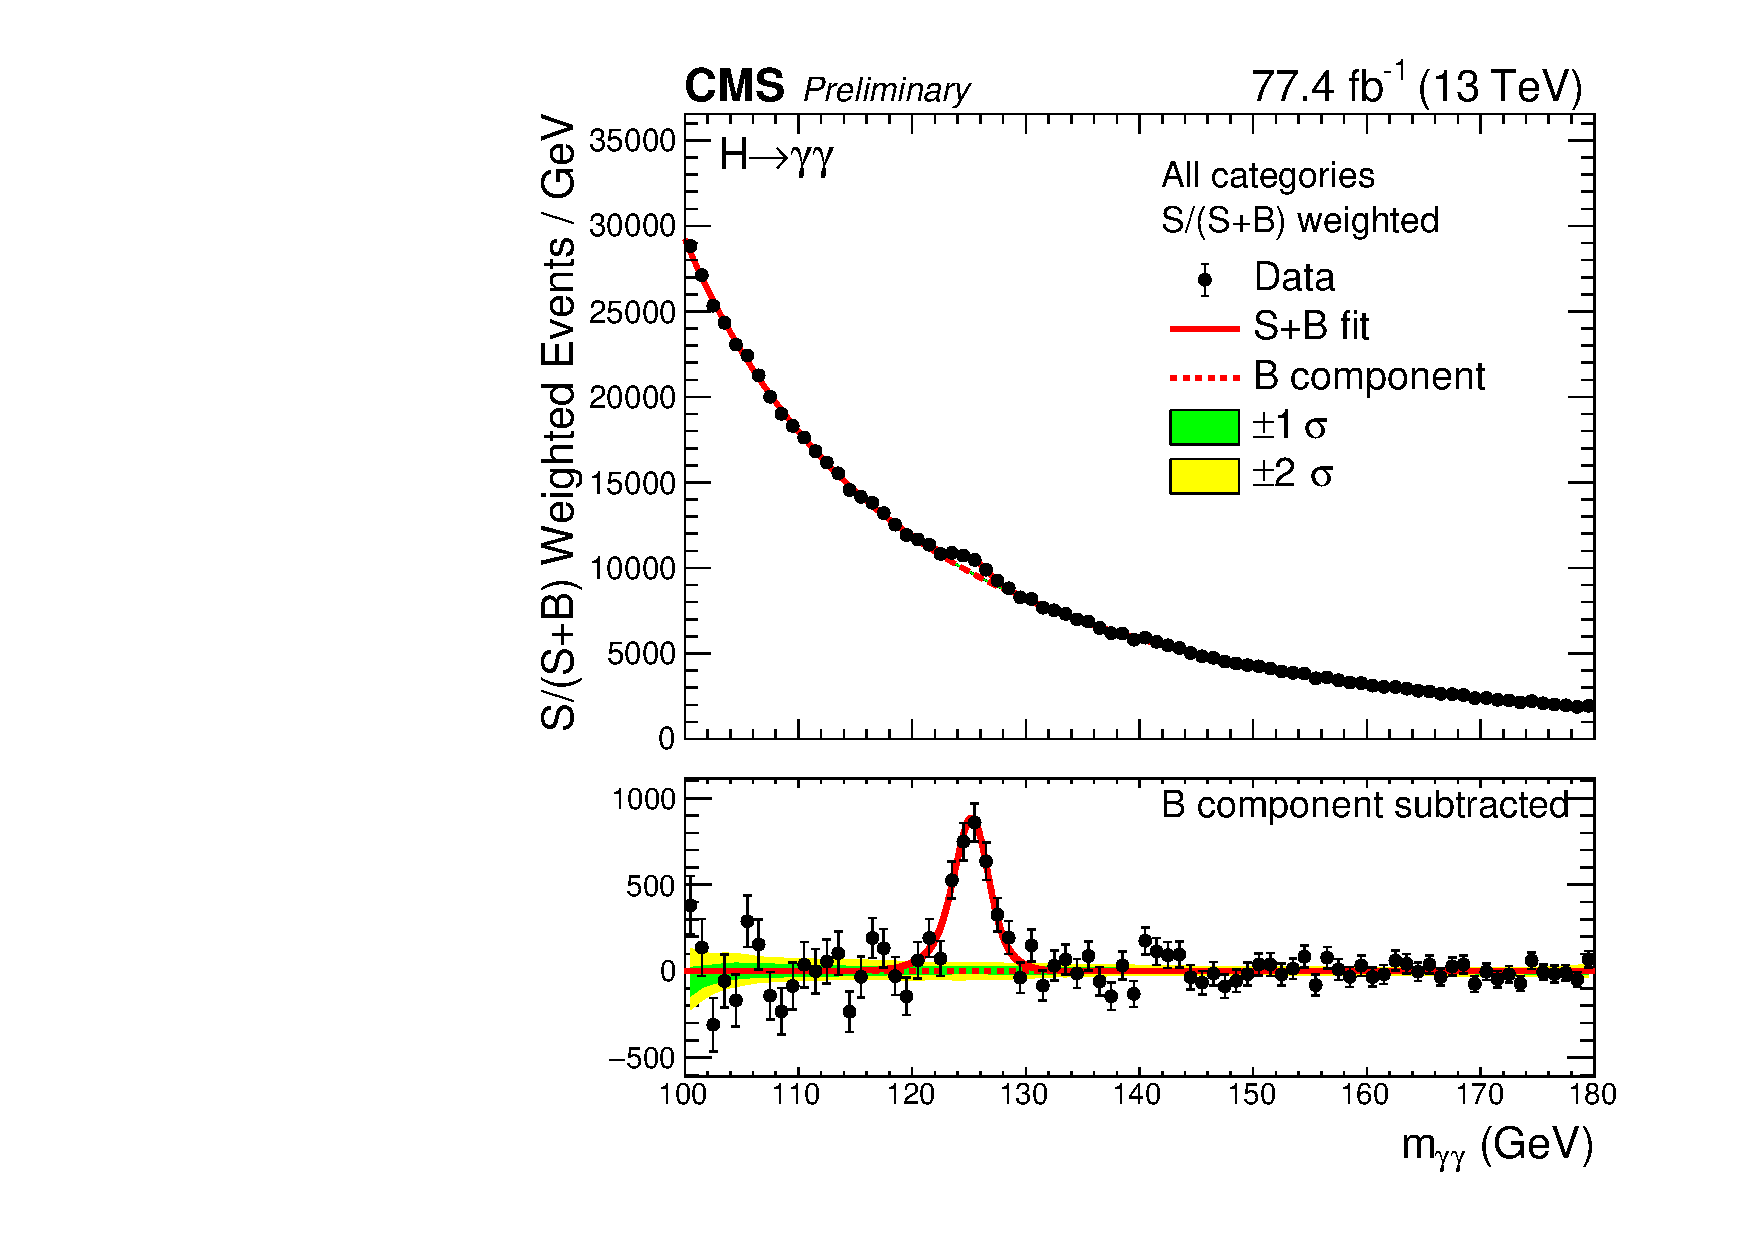
\includegraphics[width=\textwidth]{Figures/Results/MassPlot.pdf}
  \caption[Signal plus background fit to data, summed over all analysis categories.]
  {
    Data points (black) and signal plus background model fit 
    for the sum of all analysis categories is shown. 
    Each category is weighted by S/(S + B), 
    where S and B are the numbers of expected signal and background events, respectively, 
    in a $\pm 1 \seff$ mass window centred on \mH. 
    The one standard deviation (green) and two standard deviation (yellow) bands 
    include the uncertainties in the background component of the fit. 
    The solid red line shows the contribution from the total signal, plus the background contribution. 
    The dashed red line shows the contribution from the background component of the fit. 
    The bottom plot shows the residuals after subtraction of this background component.
    Figure first shown in Ref.~\cite{HIG-18-029}.
  }
  \label{fig:results_MassPlot}
\end{figure}

\begin{figure}[hptb]
  \centering
  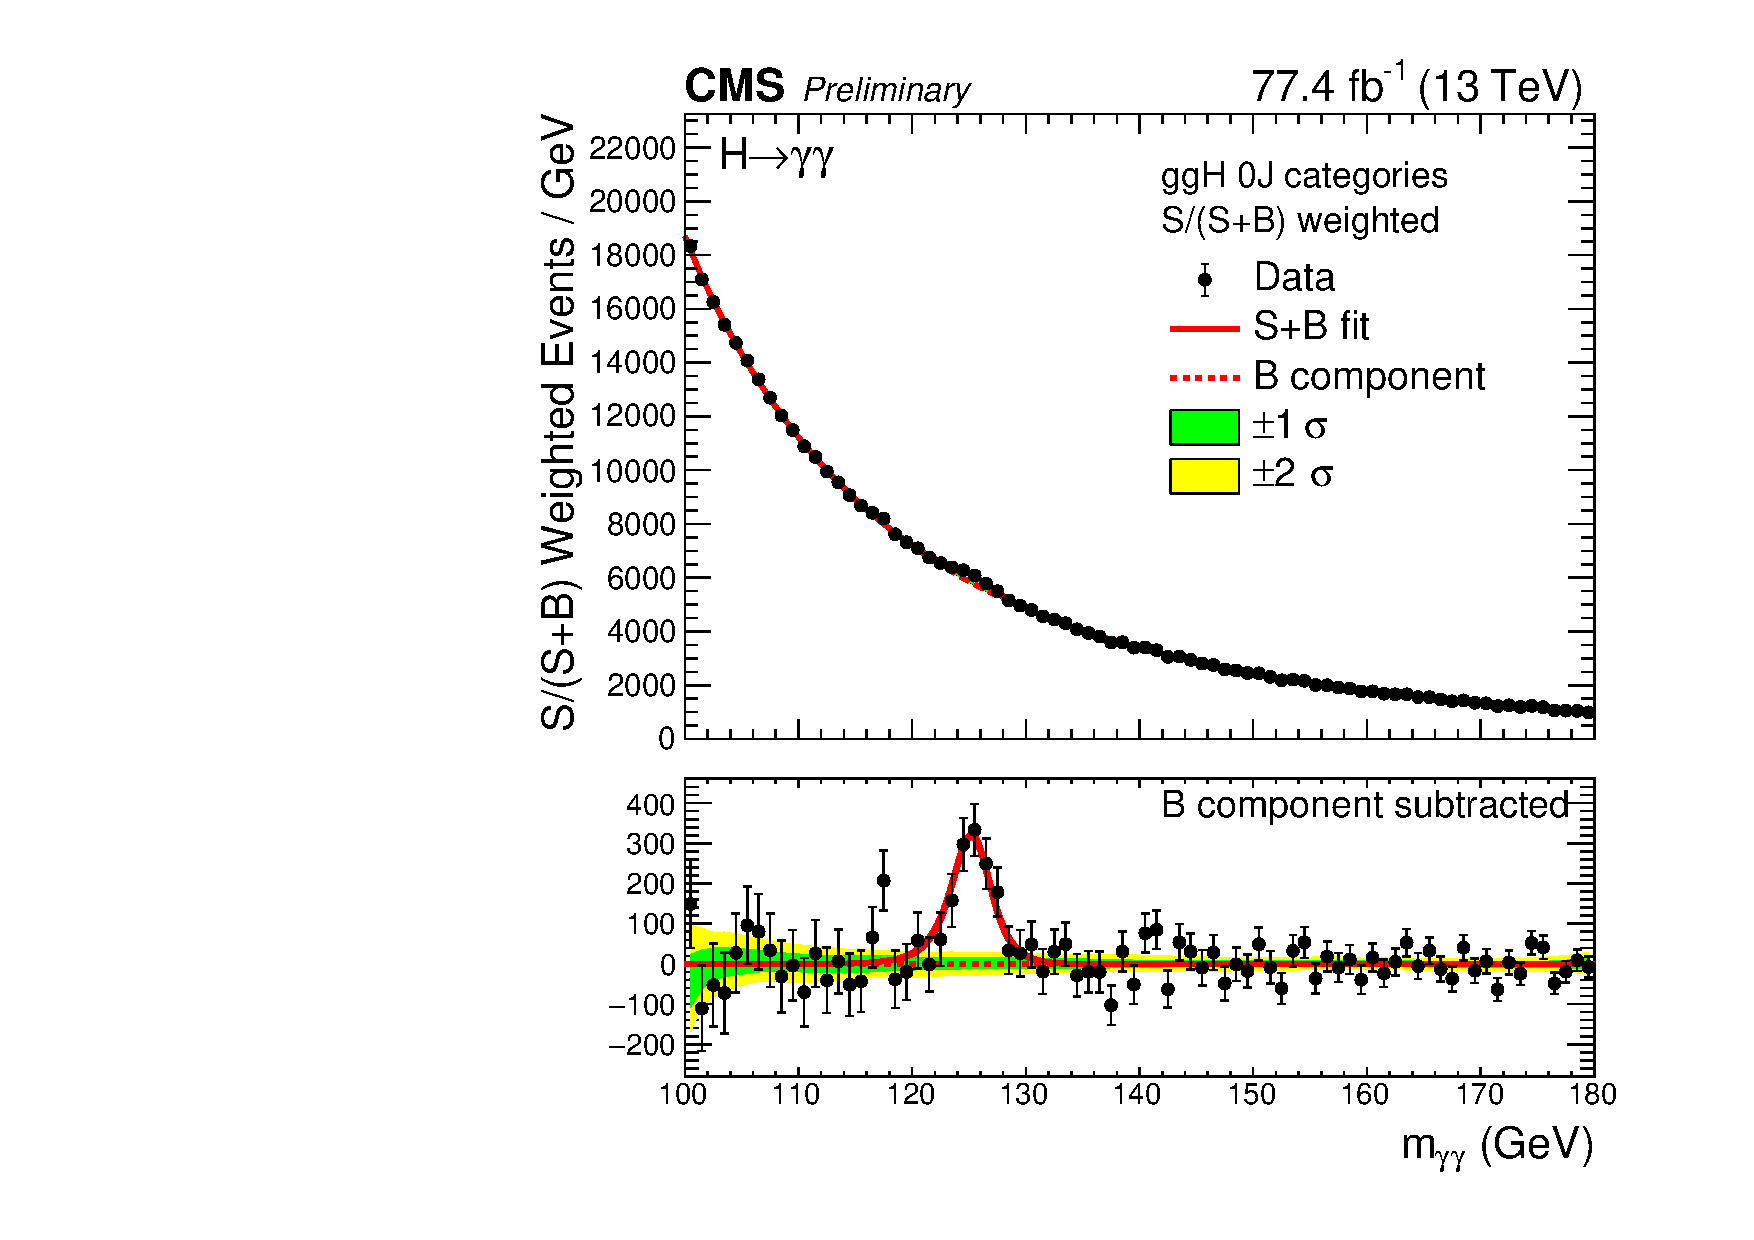
\includegraphics[width=0.49\textwidth]{Figures/Results/MassPlot_0J.pdf}
  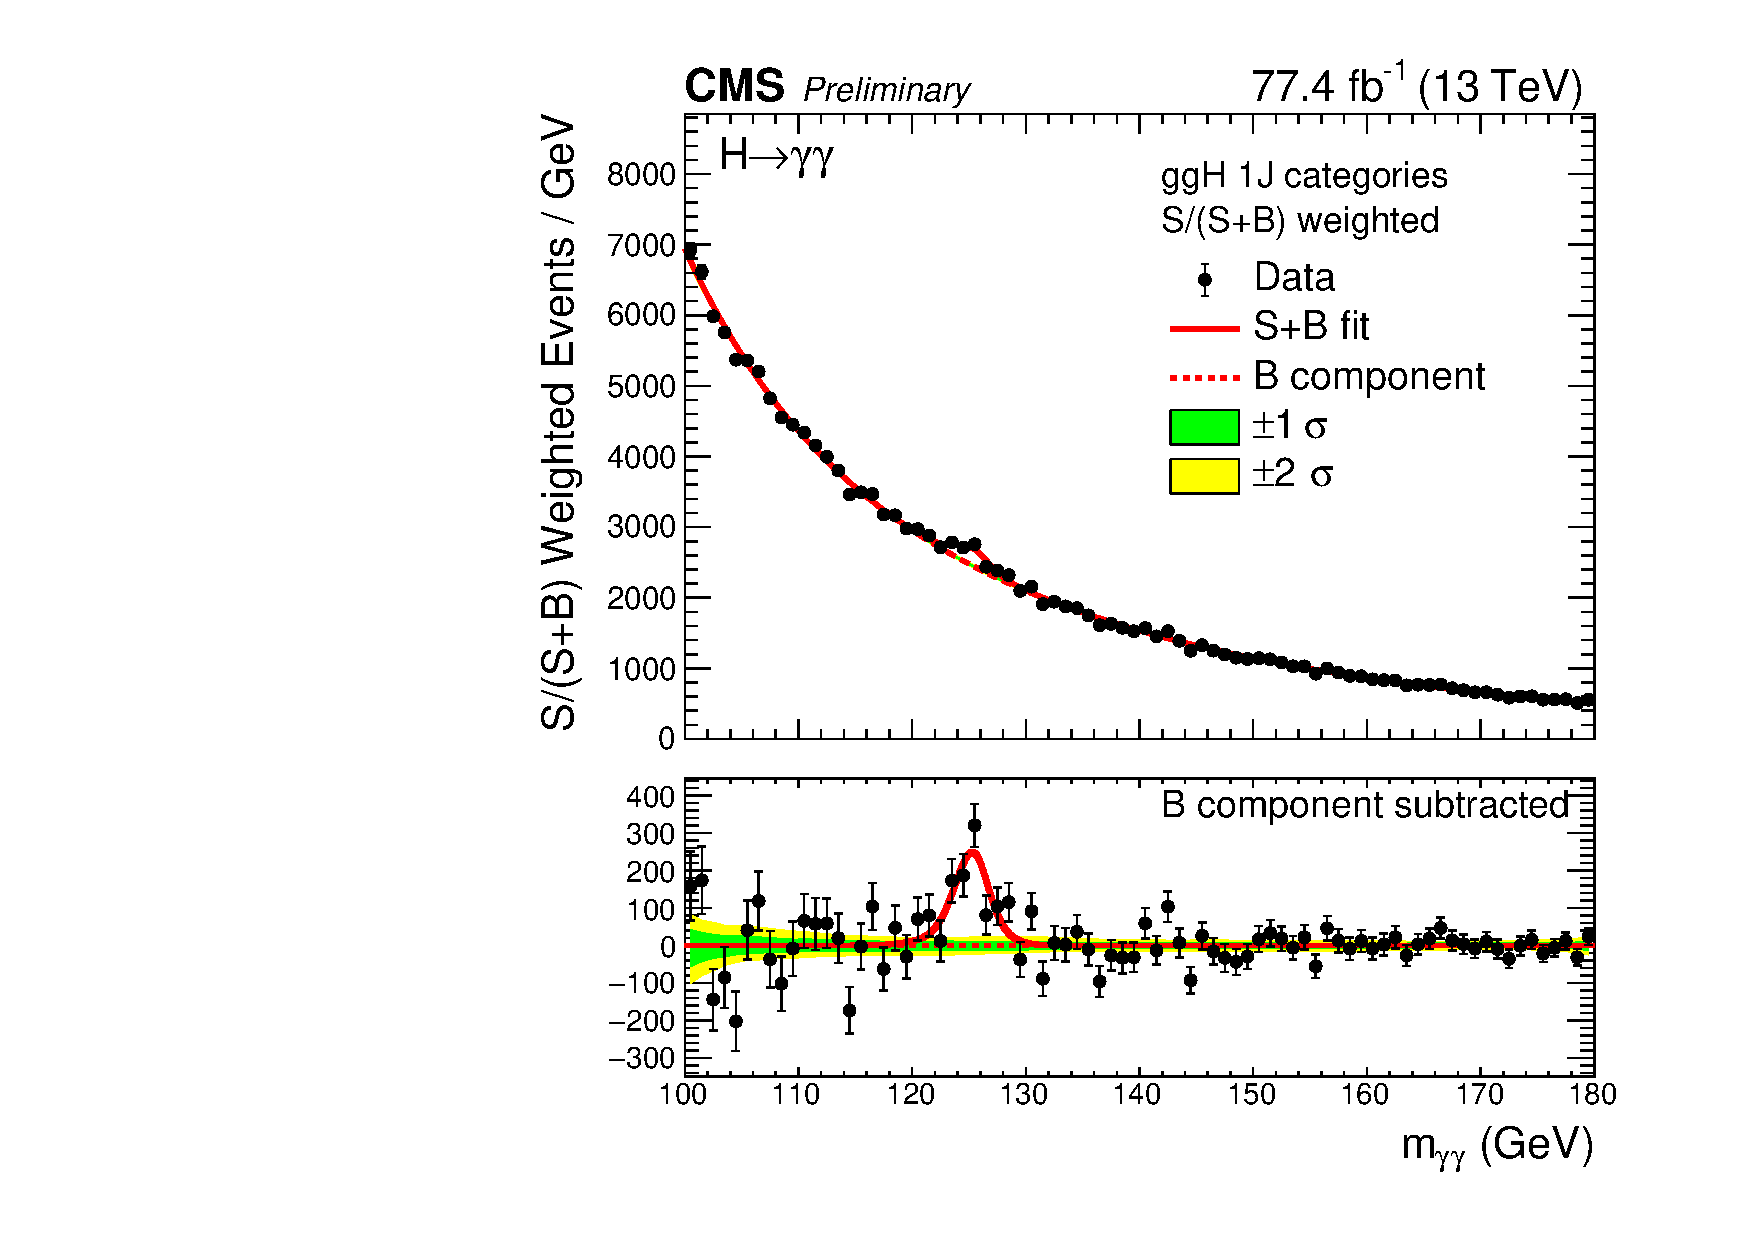
\includegraphics[width=0.49\textwidth]{Figures/Results/MassPlot_1J.pdf} \\
  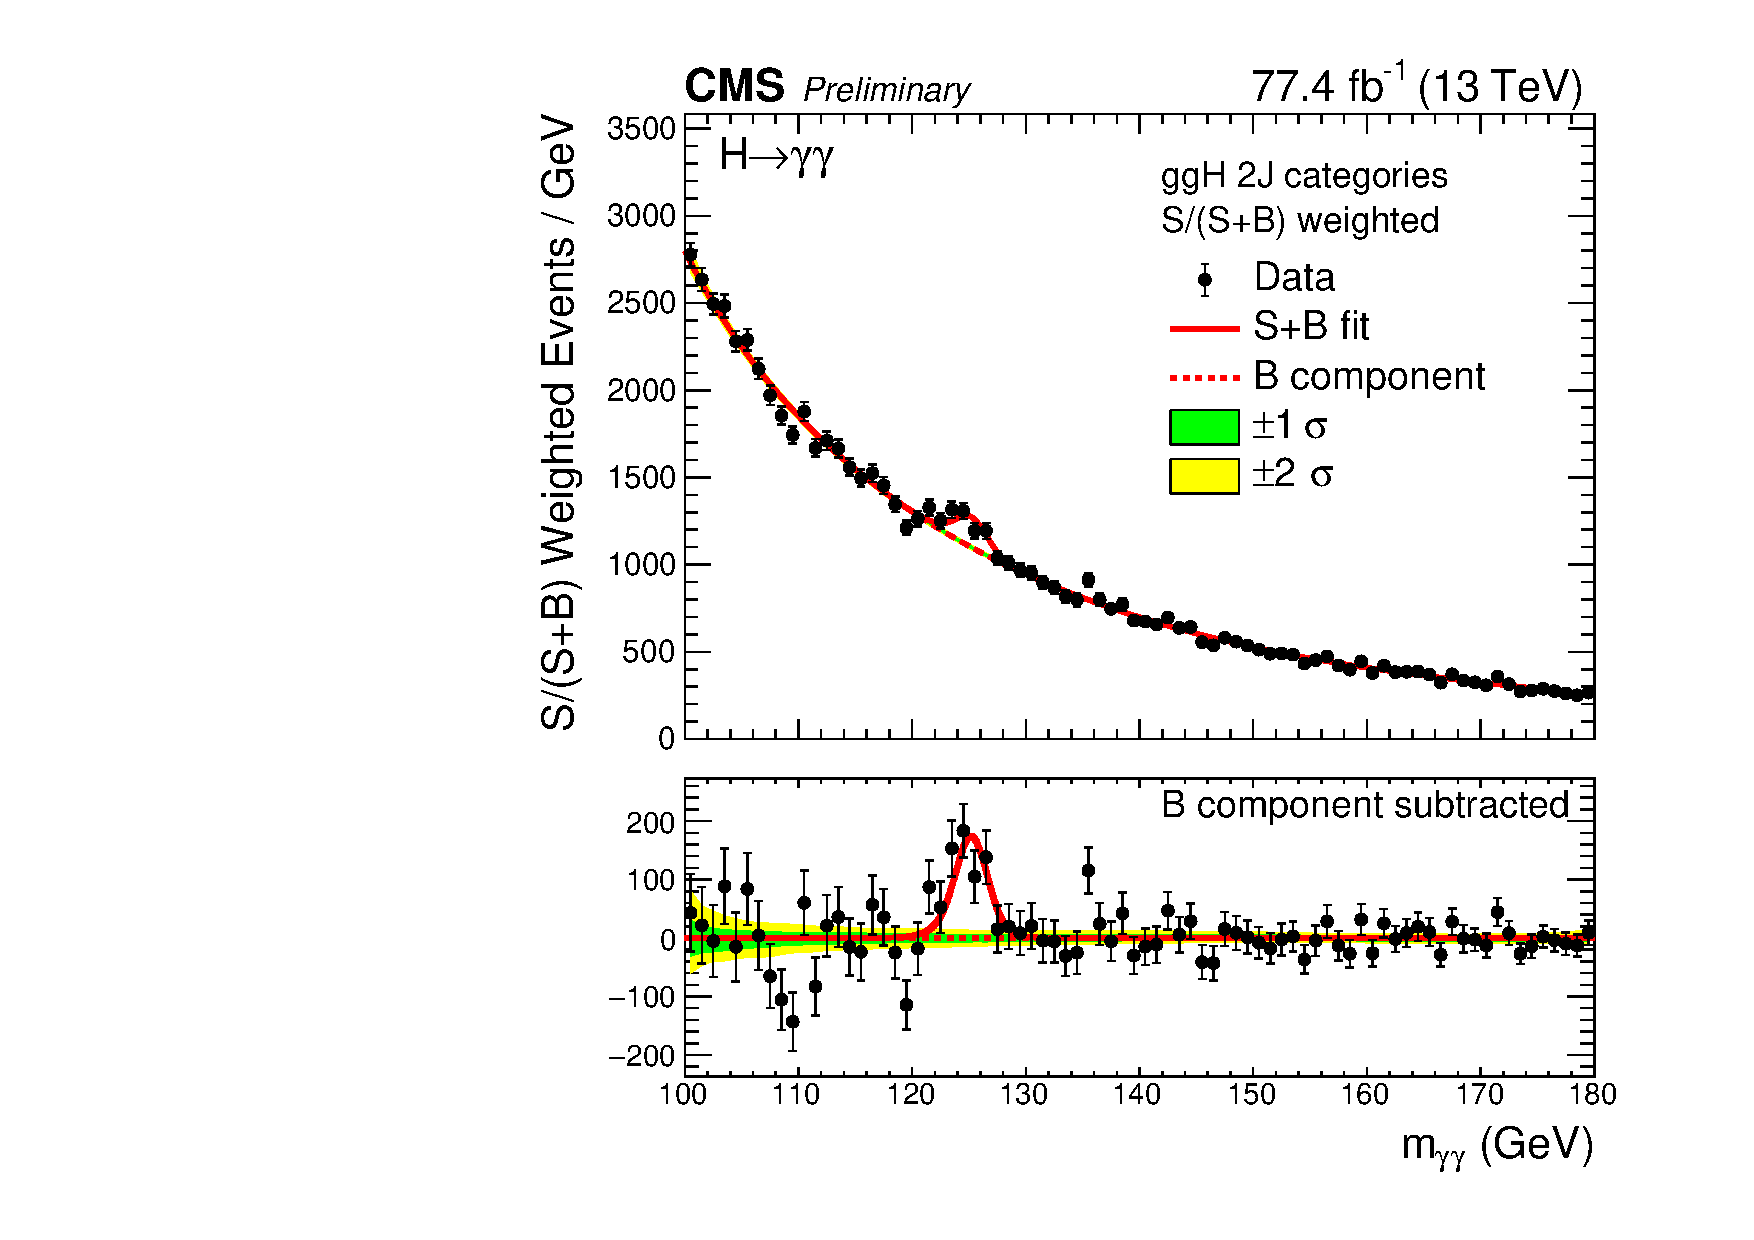
\includegraphics[width=0.49\textwidth]{Figures/Results/MassPlot_2J.pdf}
  \includegraphics[width=0.49\textwidth]{Figures/Results/MassPlot_VBF.pdf}
  \caption[Signal plus background fits to data, 
           summed over analysis categories targeting different bins.]
  {
    Data points (black) and signal plus background model fit 
    for the ggH 0J, ggH 1J, ggH 2J, and VBF categories is shown. 
    Each category is weighted by S/(S + B), 
    where S and B are the numbers of expected signal and background events, respectively, 
    in a $\pm 1 \seff$ mass window centred on \mH. 
    The one standard deviation (green) and two standard deviation (yellow) bands 
    include the uncertainties in the background component of the fit. 
    The solid red line shows the contribution from the total signal, plus the background contribution. 
    The dashed red line shows the contribution from the background component of the fit. 
    The bottom plot shows the residuals after subtraction of this background component.
  }
  \label{fig:results_MassPlots}
\end{figure}

\section{Composition of analysis categories}

All analysis categories are contaminated, to varying extents, 
by background events and other signal processes which are not being targeted.
The level of contamination then affects the sensitivity of the analysis 
when the final fits are performed.
Tables~\ref{tab:results_yields2016} and \ref{tab:results_yields2017} 
show the expected number of signal events for the 2016 and 2017 datasets respectively.
The relative contribution to each category from each of the individual stage 0 bins is shown, 
together with the \seff and \shm (the FWHM divided by 2.35) for the category's signal model.
Also reported is the expected number of background events per GeV in a $\pm1\seff$ window 
around \SI{125}{GeV}, calculated using the best-fit background function.
The table illustrates how the ratio of expected ratio of signal 
to signal plus background events (S/S+B) is highest in the ``Tag 0" categories, 
with lower S/S+B values but a greater number of events overall as the tag number increases.

The signal composition of the analysis categories in terms of the stage 1 bins being targeted
is shown in Figures~\ref{fig:results_Cats2016} and \ref{fig:results_Cats2017}.
The contribution of each bin to the total number of expected signal events in a category is displayed, 
meaning the values in each row sum to 100\%.
In general the migration between categories due to mis-measurement of \ptgg is very low, 
whilst there are significantly higher migrations arising from jet counting.

\begin{figure}[hptb]
  \centering
  \includegraphics[width=\textwidth]{Figures/Results/Cats2016.pdf}
  \caption[Signal composition of 2016 analysis categories.]
  {
    The composition of each analysis category in terms of stage 1 bins is shown. 
    The colour scale corresponds to the fraction of each category (rows) 
    accounted for by each stage 1 process (columns). 
    Each row therefore sums to 100\%. 
    Entries with values less than 0.5\% are not shown. 
    Simulation corresponding to 2016 conditions is shown.
    Figure first shown in Ref.~\cite{HIG-18-029}.
  }
  \label{fig:results_Cats2016}
\end{figure}

\begin{figure}[hptb]
  \centering
  \includegraphics[width=\textwidth]{Figures/Results/Cats2017.pdf}
  \caption[Signal composition of 2017 analysis categories.]
  {
    The composition of each analysis category in terms of stage 1 bins is shown. 
    The colour scale corresponds to the fraction of each category (rows) 
    accounted for by each stage 1 process (columns). 
    Each row therefore sums to 100\%. 
    Entries with values less than 0.5\% are not shown. 
    Simulation corresponding to 2017 conditions is shown.
    Figure first shown in Ref.~\cite{HIG-18-029}.
  }
  \label{fig:results_Cats2017}
\end{figure}

\begin{landscape}
  \begin{table}
    \resizebox{1.5\textwidth}{!}{\begin{tabular}{ r | c | c | c  | c | c |  c |  c |  c |  c |  c |  c |  c |  c |  c |  c |  c }
\hline
\multirow{2}{*}{Event Categories} &\multicolumn{14}{|c|}{SM 125 GeV Higgs boson expected signal} & Bkg & S/(S+B) \\ \cline{2-15}
  &  Total & ggH & VBF & ttH & tHq & tHW & bbH & ggZH & WH lep & WH had & ZH lep & ZH had &   $\sigma_{eff} $  & $\sigma_{HM} $ & (GeV$^{-1}$) & \\ 
\hline
 0J Tag 0 &  257.1  &  95.0 \%  &  1.9 \%  &  $<$0.05 \%  &  $<$0.05 \%  &  $<$0.05 \%  &  0.9 \%  &  0.1 \%  &  0.9 \%  &  0.3 \%  &  0.7 \%  &  0.2 \%  & 1.66 & 1.48 & 522.7 & 0.09 \\
 0J Tag 1 &  356.4  &  96.0 \%  &  1.6 \%  &  $<$0.05 \%  &  $<$0.05 \%  &  $<$0.05 \%  &  0.9 \%  &  $<$0.05 \%  &  0.6 \%  &  0.4 \%  &  0.4 \%  &  0.2 \%  & 2.10 & 1.74 & 1182.2 & 0.05 \\
 0J Tag 2 &  417.2  &  96.5 \%  &  1.4 \%  &  $<$0.05 \%  &  $<$0.05 \%  &  $<$0.05 \%  &  0.8 \%  &  $<$0.05 \%  &  0.6 \%  &  0.3 \%  &  0.3 \%  &  0.2 \%  & 2.38 & 1.97 & 3229.8 & 0.02 \\
 1J Low Tag 0 &  115.1  &  88.9 \%  &  6.5 \%  &  0.1 \%  &  $<$0.05 \%  &  $<$0.05 \%  &  1.3 \%  &  $<$0.05 \%  &  0.6 \%  &  1.4 \%  &  0.2 \%  &  0.8 \%  & 1.61 & 1.37 & 269.6 & 0.08 \\
 1J Low Tag 1 &  145.5  &  89.2 \%  &  6.2 \%  &  0.1 \%  &  $<$0.05 \%  &  $<$0.05 \%  &  1.2 \%  &  $<$0.05 \%  &  0.6 \%  &  1.6 \%  &  0.3 \%  &  0.9 \%  & 2.13 & 1.82 & 722.3 & 0.03 \\
 1J Medium Tag 0 &  48.7  &  79.9 \%  &  13.7 \%  &  0.1 \%  &  0.1 \%  &  $<$0.05 \%  &  0.8 \%  &  0.3 \%  &  1.1 \%  &  2.2 \%  &  0.4 \%  &  1.4 \%  & 1.54 & 1.40 & 61.4 & 0.15 \\
 1J Medium Tag 1 &  109.1  &  81.1 \%  &  12.6 \%  &  0.1 \%  &  0.1 \%  &  $<$0.05 \%  &  0.9 \%  &  0.1 \%  &  1.0 \%  &  2.2 \%  &  0.5 \%  &  1.4 \%  & 1.86 & 1.61 & 383.9 & 0.05 \\
 1J High Tag 0 &  17.6  &  70.3 \%  &  19.8 \%  &  0.2 \%  &  0.1 \%  &  $<$0.05 \%  &  0.5 \%  &  0.7 \%  &  2.7 \%  &  2.9 \%  &  1.0 \%  &  1.7 \%  & 1.47 & 1.34 & 15.6 & 0.21 \\
 1J High Tag 1 &  21.2  &  70.8 \%  &  19.5 \%  &  0.3 \%  &  0.1 \%  &  $<$0.05 \%  &  0.4 \%  &  0.9 \%  &  2.5 \%  &  2.7 \%  &  1.1 \%  &  1.7 \%  & 1.74 & 1.64 & 61.3 & 0.06 \\
 1J BSM &  8.6  &  63.9 \%  &  21.6 \%  &  0.3 \%  &  0.2 \%  &  0.1 \%  &  0.3 \%  &  1.6 \%  &  4.9 \%  &  3.4 \%  &  2.0 \%  &  1.8 \%  & 1.40 & 1.35 & 6.0 & 0.26 \\
 2J Low Tag 0 &  28.8  &  75.7 \%  &  8.2 \%  &  4.2 \%  &  0.5 \%  &  $<$0.05 \%  &  3.0 \%  &  0.1 \%  &  0.9 \%  &  4.1 \%  &  0.5 \%  &  2.7 \%  & 1.61 & 1.21 & 86.2 & 0.07 \\
 2J Low Tag 1 &  38.5  &  73.3 \%  &  10.3 \%  &  4.2 \%  &  0.5 \%  &  $<$0.05 \%  &  2.7 \%  &  0.3 \%  &  0.9 \%  &  4.5 \%  &  0.5 \%  &  2.8 \%  & 1.98 & 1.70 & 254.7 & 0.03 \\
 2J Medium Tag 0 &  24.8  &  72.1 \%  &  9.6 \%  &  5.0 \%  &  0.6 \%  &  0.1 \%  &  1.7 \%  &  0.6 \%  &  0.8 \%  &  5.7 \%  &  0.5 \%  &  3.3 \%  & 1.50 & 1.36 & 38.7 & 0.13 \\
 2J Medium Tag 1 &  50.5  &  68.8 \%  &  11.2 \%  &  6.0 \%  &  0.6 \%  &  0.1 \%  &  2.1 \%  &  0.7 \%  &  0.9 \%  &  5.7 \%  &  0.5 \%  &  3.3 \%  & 1.85 & 1.54 & 213.2 & 0.04 \\
 2J High Tag 0 &  22.6  &  65.3 \%  &  11.2 \%  &  7.3 \%  &  1.0 \%  &  0.3 \%  &  0.9 \%  &  1.4 \%  &  1.4 \%  &  6.9 \%  &  0.5 \%  &  3.8 \%  & 1.52 & 1.41 & 21.7 & 0.19 \\
 2J High Tag 1 &  28.4  &  65.0 \%  &  11.9 \%  &  7.8 \%  &  0.9 \%  &  0.2 \%  &  1.0 \%  &  1.7 \%  &  1.1 \%  &  6.4 \%  &  0.5 \%  &  3.6 \%  & 1.78 & 1.72 & 79.8 & 0.06 \\
 2J BSM Tag 0 &  14.6  &  56.3 \%  &  11.1 \%  &  11.5 \%  &  1.9 \%  &  1.2 \%  &  0.3 \%  &  2.6 \%  &  1.5 \%  &  8.1 \%  &  0.7 \%  &  4.9 \%  & 1.40 & 1.33 & 6.5 & 0.35 \\
 2J BSM Tag 1 &  9.7  &  57.8 \%  &  11.5 \%  &  12.1 \%  &  1.6 \%  &  0.9 \%  &  0.4 \%  &  1.4 \%  &  1.6 \%  &  7.7 \%  &  0.7 \%  &  4.2 \%  & 1.64 & 1.53 & 17.3 & 0.10 \\
 VBF 2J-like Tag 0 &  12.9  &  19.5 \%  &  79.8 \%  &  0.1 \%  &  0.1 \%  &  $<$0.05 \%  &  0.3 \%  &  0.1 \%  &  0.1 \%  &  0.1 \%  &  $<$0.05 \%  &  $<$0.05 \%  & 1.70 & 1.41 & 4.9 & 0.35 \\
 VBF 2J-like Tag 1 &  6.2  &  32.4 \%  &  65.5 \%  &  0.3 \%  &  0.2 \%  &  $<$0.05 \%  &  0.7 \%  &  0.1 \%  &  0.2 \%  &  0.5 \%  &  $<$0.05 \%  &  0.1 \%  & 1.85 & 1.52 & 8.4 & 0.12 \\
 VBF 3J-like Tag 0 &  12.0  &  30.6 \%  &  65.6 \%  &  1.3 \%  &  0.7 \%  &  0.1 \%  &  0.8 \%  &  0.4 \%  &  0.1 \%  &  0.3 \%  &  $<$0.05 \%  &  0.2 \%  & 1.59 & 1.34 & 6.0 & 0.30 \\
 VBF 3J-like Tag 1 &  13.6  &  52.5 \%  &  38.9 \%  &  3.2 \%  &  1.2 \%  &  0.1 \%  &  1.1 \%  &  0.4 \%  &  0.5 \%  &  1.1 \%  &  0.3 \%  &  0.7 \%  & 1.71 & 1.51 & 19.5 & 0.12 \\
 VBF Rest &  13.0  &  59.5 \%  &  29.4 \%  &  3.5 \%  &  1.0 \%  &  0.2 \%  &  1.4 \%  &  0.7 \%  &  1.0 \%  &  2.0 \%  &  0.3 \%  &  1.0 \%  & 1.50 & 1.29 & 21.2 & 0.12 \\
 VBF BSM &  7.2  &  45.5 \%  &  39.9 \%  &  6.5 \%  &  1.0 \%  &  0.8 \%  &  0.9 \%  &  1.1 \%  &  1.0 \%  &  2.2 \%  &  0.1 \%  &  1.0 \%  & 1.48 & 1.29 & 6.0 & 0.22 \\
Total &    1779.2  &  87.5 \%  &  6.7 \%  &  0.9 \%  &  0.1 \%  &  $<$0.05 \%  &  1.0 \%  &  0.2 \%  &  0.8 \%  &  1.4 \%  &  0.4 \%  &  0.8 \%  & 1.96 & 1.67 & 7238.9 & 0.04 \\
\hline
\end{tabular}
}
    \caption[Signal and background yields for 2016 analysis categories.]
    {
      The expected number of signal events per category and
      the percentage breakdown per production mode in that category. 
      The $\sigma_{eff}$, computed as the smallest interval containing 68.3\% 
      of the invariant mass distribution, and $\sigma_{HM}$, computed as the FWHM divided by 2.35,
      are also shown as an estimate of the \mgg resolution in that category.
      The expected number of background events per GeV around 125 GeV is listed.
      The expected ratio of signal to signal plus background events, S/(S + B), is also shown,
      where S and B are the numbers of expected signal and background events, respectively, 
      in a $\pm 1 \sigma_{eff}$ mass window centred on \mH.
      Data and simulation from 2016 are shown.
    }
    \label{tab:results_yields2016}
  \end{table}
\end{landscape}

\begin{landscape}
  \begin{table}
    \resizebox{1.5\textwidth}{!}{\begin{tabular}{ r | c | c | c  | c | c |  c |  c |  c |  c |  c |  c |  c |  c |  c |  c |  c }
\hline
\multirow{2}{*}{Event Categories} &\multicolumn{14}{|c|}{SM 125 GeV Higgs boson expected signal} & Bkg & S/(S+B) \\ \cline{2-15}
  &  Total & ggH & VBF & ttH & tHq & tHW & bbH & ggZH & WH lep & WH had & ZH lep & ZH had &   $\sigma_{eff} $  & $\sigma_{HM} $ & (GeV$^{-1}$) & \\ 
\hline
 0J Tag 0 &  401.1  &  91.8 \%  &  4.4 \%  &  $<$0.05 \%  &  $<$0.05 \%  &  $<$0.05 \%  &  1.4 \%  &  0.1 \%  &  1.0 \%  &  0.4 \%  &  0.6 \%  &  0.2 \%  & 1.94 & 1.79 & 870.3 & 0.07 \\
 0J Tag 1 &  552.3  &  93.7 \%  &  3.1 \%  &  $<$0.05 \%  &  $<$0.05 \%  &  $<$0.05 \%  &  1.3 \%  &  $<$0.05 \%  &  0.7 \%  &  0.4 \%  &  0.4 \%  &  0.2 \%  & 2.42 & 2.06 & 2121.9 & 0.04 \\
 0J Tag 2 &  347.3  &  95.0 \%  &  2.2 \%  &  $<$0.05 \%  &  $<$0.05 \%  &  $<$0.05 \%  &  1.3 \%  &  $<$0.05 \%  &  0.5 \%  &  0.4 \%  &  0.3 \%  &  0.2 \%  & 2.72 & 2.41 & 3035.8 & 0.01 \\
 1J Low Tag 0 &  130.8  &  89.5 \%  &  5.9 \%  &  0.1 \%  &  $<$0.05 \%  &  $<$0.05 \%  &  1.1 \%  &  $<$0.05 \%  &  0.5 \%  &  1.7 \%  &  0.2 \%  &  0.9 \%  & 1.91 & 1.71 & 360.2 & 0.06 \\
 1J Low Tag 1 &  111.5  &  89.2 \%  &  6.1 \%  &  0.1 \%  &  $<$0.05 \%  &  $<$0.05 \%  &  1.1 \%  &  $<$0.05 \%  &  0.5 \%  &  1.8 \%  &  0.2 \%  &  1.0 \%  & 2.47 & 2.22 & 689.4 & 0.02 \\
 1J Medium Tag 0 &  71.4  &  81.5 \%  &  12.4 \%  &  0.2 \%  &  0.1 \%  &  $<$0.05 \%  &  0.5 \%  &  0.2 \%  &  0.9 \%  &  2.5 \%  &  0.4 \%  &  1.3 \%  & 1.85 & 1.67 & 110.8 & 0.11 \\
 1J Medium Tag 1 &  91.1  &  82.7 \%  &  11.4 \%  &  0.2 \%  &  0.1 \%  &  $<$0.05 \%  &  0.5 \%  &  0.2 \%  &  0.8 \%  &  2.3 \%  &  0.4 \%  &  1.4 \%  & 2.13 & 1.91 & 342.2 & 0.04 \\
 1J High Tag 0 &  14.7  &  71.7 \%  &  19.4 \%  &  0.3 \%  &  0.2 \%  &  $<$0.05 \%  &  0.3 \%  &  1.0 \%  &  2.3 \%  &  2.5 \%  &  1.0 \%  &  1.5 \%  & 1.54 & 1.51 & 8.7 & 0.27 \\
 1J High Tag 1 &  28.2  &  72.4 \%  &  18.4 \%  &  0.4 \%  &  0.2 \%  &  $<$0.05 \%  &  0.3 \%  &  0.8 \%  &  2.2 \%  &  2.8 \%  &  0.9 \%  &  1.7 \%  & 1.76 & 1.77 & 47.7 & 0.10 \\
 1J BSM &  15.5  &  66.9 \%  &  20.9 \%  &  0.4 \%  &  0.3 \%  &  0.1 \%  &  0.1 \%  &  1.0 \%  &  4.0 \%  &  3.0 \%  &  1.6 \%  &  1.8 \%  & 1.76 & 1.71 & 17.5 & 0.15 \\
 2J Low Tag 0 &  10.9  &  80.2 \%  &  7.0 \%  &  1.7 \%  &  0.4 \%  &  $<$0.05 \%  &  1.0 \%  &  0.3 \%  &  0.7 \%  &  4.8 \%  &  0.3 \%  &  3.4 \%  & 1.55 & 1.52 & 35.1 & 0.06 \\
 2J Low Tag 1 &  40.8  &  77.6 \%  &  8.1 \%  &  3.0 \%  &  0.5 \%  &  $<$0.05 \%  &  0.8 \%  &  0.3 \%  &  0.7 \%  &  5.4 \%  &  0.3 \%  &  3.1 \%  & 2.06 & 1.94 & 249.0 & 0.03 \\
 2J Medium Tag 0 &  16.8  &  76.6 \%  &  8.1 \%  &  1.9 \%  &  0.5 \%  &  0.1 \%  &  0.3 \%  &  1.0 \%  &  0.7 \%  &  7.0 \%  &  0.4 \%  &  3.4 \%  & 1.60 & 1.46 & 28.9 & 0.11 \\
 2J Medium Tag 1 &  49.7  &  74.6 \%  &  9.1 \%  &  3.4 \%  &  0.6 \%  &  0.1 \%  &  0.4 \%  &  0.8 \%  &  0.9 \%  &  6.1 \%  &  0.4 \%  &  3.6 \%  & 2.12 & 1.86 & 228.8 & 0.03 \\
 2J High Tag 0 &  14.0  &  71.1 \%  &  9.2 \%  &  1.7 \%  &  0.6 \%  &  0.1 \%  &  0.2 \%  &  2.7 \%  &  1.0 \%  &  8.2 \%  &  0.7 \%  &  4.6 \%  & 1.54 & 1.52 & 14.2 & 0.18 \\
 2J High Tag 1 &  24.4  &  69.1 \%  &  9.4 \%  &  3.7 \%  &  0.8 \%  &  0.2 \%  &  0.2 \%  &  2.3 \%  &  1.1 \%  &  8.2 \%  &  0.5 \%  &  4.7 \%  & 1.42 & 1.31 & 64.4 & 0.08 \\
 2J BSM Tag 0 &  15.8  &  66.4 \%  &  9.4 \%  &  2.6 \%  &  0.9 \%  &  0.4 \%  &  0.1 \%  &  2.7 \%  &  1.9 \%  &  9.3 \%  &  0.9 \%  &  5.4 \%  & 1.67 & 1.63 & 11.1 & 0.22 \\
 2J BSM Tag 1 &  5.7  &  60.4 \%  &  9.5 \%  &  9.2 \%  &  1.4 \%  &  0.7 \%  &  0.1 \%  &  2.7 \%  &  1.4 \%  &  9.0 \%  &  1.0 \%  &  4.7 \%  & 1.89 & 1.82 & 24.3 & 0.04 \\
 VBF 2J-like Tag 0 &  13.5  &  24.8 \%  &  74.4 \%  &  0.1 \%  &  0.1 \%  &  $<$0.05 \%  &  0.1 \%  &  0.1 \%  &  $<$0.05 \%  &  0.2 \%  &  $<$0.05 \%  &  0.2 \%  & 1.90 & 1.73 & 5.7 & 0.30 \\
 VBF 2J-like Tag 1 &  4.8  &  41.7 \%  &  56.5 \%  &  0.2 \%  &  0.2 \%  &  $<$0.05 \%  &  0.2 \%  &  0.2 \%  &  0.2 \%  &  0.5 \%  &  $<$0.05 \%  &  0.3 \%  & 2.28 & 1.94 & 9.3 & 0.07 \\
 VBF 3J-like Tag 0 &  12.7  &  36.8 \%  &  60.6 \%  &  0.4 \%  &  0.5 \%  &  $<$0.05 \%  &  0.1 \%  &  0.4 \%  &  0.2 \%  &  0.5 \%  &  0.1 \%  &  0.2 \%  & 1.90 & 1.69 & 7.8 & 0.23 \\
 VBF 3J-like Tag 1 &  7.6  &  56.0 \%  &  37.8 \%  &  0.8 \%  &  0.9 \%  &  $<$0.05 \%  &  0.2 \%  &  0.8 \%  &  0.5 \%  &  1.6 \%  &  0.2 \%  &  1.0 \%  & 1.86 & 1.79 & 11.1 & 0.11 \\
 VBF Rest &  12.9  &  63.4 \%  &  29.9 \%  &  1.0 \%  &  0.6 \%  &  0.1 \%  &  0.4 \%  &  0.8 \%  &  0.6 \%  &  2.0 \%  &  0.3 \%  &  1.1 \%  & 1.80 & 1.71 & 21.3 & 0.10 \\
 VBF BSM &  6.5  &  44.7 \%  &  47.8 \%  &  1.0 \%  &  0.5 \%  &  0.3 \%  &  0.1 \%  &  1.4 \%  &  0.7 \%  &  2.1 \%  &  0.4 \%  &  1.0 \%  & 1.75 & 1.45 & 4.5 & 0.22 \\
Total &    1999.8  &  88.2 \%  &  6.7 \%  &  0.4 \%  &  0.1 \%  &  $<$0.05 \%  &  1.1 \%  &  0.2 \%  &  0.8 \%  &  1.4 \%  &  0.4 \%  &  0.8 \%  & 2.22 & 1.98 & 8320.2 & 0.04 \\
\hline
\end{tabular}
}
    \caption[Signal and background yields for 2017 analysis categories.]
    {
      The expected number of signal events per category and
      the percentage breakdown per production mode in that category. 
      The $\sigma_{eff}$, computed as the smallest interval containing 68.3\% 
      of the invariant mass distribution, and $\sigma_{HM}$, computed as the FWHM divided by 2.35,
      are also shown as an estimate of the \mgg resolution in that category.
      The expected number of background events per GeV around 125 GeV is listed.
      The expected ratio of signal to signal plus background events, S/(S + B), is also shown,
      where S and B are the numbers of expected signal and background events, respectively, 
      in a $\pm 1 \sigma_{eff}$ mass window centred on \mH.
      Data and simulation from 2017 are shown.
    }
    \label{tab:results_yields2017}
  \end{table}
\end{landscape}

\section{Results in the STXS framework}

Results in the STXS framework are presented with three different parameterisations;
for each result the underlying signal bins 
are grouped into different parameters which are free to vary in the fit.
The recommendations contained in Ref.~\cite{YR4} 
concerning how to treat sub-dominant processes are followed in each case.
The ggH parameters include bbH events.
The ggZH process is grouped together with leptonic VH production if the Z boson decays leptonically, 
and with ggH otherwise.
The hadronic VH processes are grouped with VBF production to form the qqH parameters.
In each fit, the ttH, tH, and VH leptonic parameters are constrained to their SM prediction. 
This is necessary since there are no categories targeting these production modes, 
and therefore the parameters would be almost unconstrained 
and cause increased uncertainties in the other parameters of interest.
In all fits the mass of the Higgs boson is profiled.

\subsection{Stage 0 cross sections}
Measurements of stage 0 STXS bins are performed in a fit with two parameters, ggH and qqH.
The resulting cross sections, normalised to the SM prediction, are found to be 
%$\sigma_{ggH}/\sigma_{ggH}^{\textrm{SM}} = 1.00 \pm 0.13$ 
%and $\sigma_{qqH}^{\textrm{SM}} = 1.0 \pm 0.4$.
$\sigma_{ggH}/\sigma_{ggH}^{\textrm{SM}} = 1.15 \pm 0.15$ 
and $\sigma_{qqH}/\sigma_{qqH}^{\textrm{SM}} = 0.83_{-0.31}^{+0.37}$.
The individual likelihood scans are shown 
in Figures~\ref{fig:results_Stage0_ggH} and \ref{fig:results_Stage0_qqH}.
Two scans are shown, one corresponding to the full fit
and one corresponding to the fit without systematic uncertainties.
The systematic component of the uncertainty is then determined 
by subtracting the statistical component from the total uncertainty.
In both measurements the statistical component of the uncertainty 
is greater than the systematic component.
However for the ggH cross section, the magnitude of each is comparable.
With the full Run 2 dataset, 
which will increase the available integrated luminosity to around \SI{137}{\fbinv}, 
the ggH measurement is likely to become systematics-dominated.

\begin{figure}[hptb]
  \centering
  \includegraphics[width=\textwidth]{Figures/Results/ObsStage0_r_ggH.pdf}
  \caption[Likelihood scan for the ggH parameter in a two-parameter fit.]
  {
    The results of a two-parameter fit in the STXS framework,
    showing the scan of the profiled likelihood ratio in the ggH cross section.
    All ggH bins are grouped together in the fit to form one parameter, 
    with all VBF bins comprising the second parameter.
    The ggH parameter includes bbH components, 
    while the qqH parameter includes the hadronic VH contribution. 
    The ttH, tH and VH leptonic processes are constrained to the SM prediction. 
    The solid black line shows the full scan, 
    whilst the dashed green line shows the scan without any systematic uncertainties included.
  }
  \label{fig:results_Stage0_ggH}
\end{figure}

\begin{figure}[hptb]
  \centering
  \includegraphics[width=\textwidth]{Figures/Results/ObsStage0_r_qqH.pdf}
  \caption[Likelihood scan for the qqH parameter in a two-parameter fit.]
  {
    The results of a two-parameter fit in the STXS framework,
    showing the scan of the profiled likelihood ratio in the qqH cross section.
    All ggH bins are grouped together in the fit to form one parameter, 
    with all VBF bins comprising the second parameter.
    The ggH parameter includes bbH components, 
    while the qqH parameter includes the hadronic VH contribution. 
    The ttH, tH and VH leptonic processes are constrained to the SM prediction. 
    The solid black line shows the full scan, 
    whilst the dashed green line shows the scan without any systematic uncertainties included.
  }
  \label{fig:results_Stage0_qqH}
\end{figure}

\subsection{Stage 1 cross sections}

Two different measurements are performed at stage 1 of the STXS framework.
In both cases, some stage 1 bins are merged 
in order to improve the statistical sensitivity of the measurement.
In the first fit, the definition of parameters is motivated by merging as few bins as possible
whilst maintaining the uncertainty on each parameter at less than 100\% of the SM predicted value.
This results in a total of seven signal parameters.
There are six ggH parameters, of which four correspond to a single stage 1 bin;
these are the zero-jet (0J), one-jet low (1J low), medium (1J med), and high (1J high) \ptH bins.
The two-jet or greater parameter (GE2J) groups together five individual stage 1 bins, 
comprising the low, medium and high \ptH bins as well as the two VBF-like bins.
The ggH BSM parameter is the sum of the one-jet and two-jet BSM bins
where $\ptH > \SI{200}{GeV}$.
Finally, the qqH parameter is unchanged from stage 0;
all five bins are grouped together.
The results of this seven-parameter fit are shown in Figure~\ref{fig:results_stage1}. 
The observed 68\% CL intervals for each parameter are compared 
to the SM predictions and their associated uncertainties.
There is very good agreement with the SM; 
the $p$-value with respect to the SM hypothesis is approximately 64\%. %TODO revise how this is done
Furthermore, for several parameters, the experimental precision is less than a factor of three 
greater than the theoretical uncertainty on the SM prediction. %CONSEQUENCES

\begin{figure}[hptb]
  \centering
  \includegraphics[width=\textwidth]{Figures/Results/Stage1.pdf}
  \caption[Results of a seven-parameter fit in the STXS framework.]
  {
    The results of a seven-parameter fit in the STXS framework. 
    The ggH 1J and 2J BSM bins are grouped together in the fit; 
    the remaining five ggH bins with two or more jets are also grouped. 
    All five VBF bins are grouped together. 
    The ggH parameters include bbH components, 
    while the qqH parameter includes the hadronic VH contribution. 
    The ttH, tH and VH leptonic processes are constrained to the SM prediction. 
    Cross section ratios are shown with approximate 68\% CL intervals (black points), 
    and compared to the SM expectations and their uncertainties (blue bands).
    The compatibility of this fit with the SM prediction, 
    expressed as a $p$-value with respect to the SM, is approximately 64\%.
    Figure first shown in Ref.~\cite{HIG-18-029}.
  }
  \label{fig:results_stage1}
\end{figure}

In the second measurement at stage 1, the fit contains thirteen signal parameters.
This choice represents the minimal possible merging of bins 
whilst retaining a reasonable sensitivity of less than around 200\% of the SM prediction.
Nine of the parameters correspond to individual ggH stage 1 bins; 
the only merged ggH parameter is the so-called ggH VBF-like parameter, 
where the 2J-like and 3J-like ggH VBF-like bins are grouped together.
For qqH, the 2J-like and 3J-like parameters represent individual bins, 
while the ``qqH other" parameter is composed of the VH-like, Rest and BSM bins.
The resulting cross sections normalised to the corresponding SM predictions 
are shown in Figure~\ref{fig:results_stage1min}.
In the fit all parameters are constrained to be non-negative -- this is necessary 
to ensure the fit converges.
The parameters whose best-fit values are constrained to be zero are known to have 68\% CL intervals 
which slightly under-cover. 
This is checked and confirmed using an ensemble of pseudo-experiments.
Therefore the compatibility of those parameters with the SM prediction is higher than 
the quoted 68\% CL intervals would imply.
The compatibility of the thirteen-parameter fit with the SM prediction, 
expressed as a $p$-value with respect to the SM hypothesis, is approximately 18\%.

\begin{figure}[hptb]
  \centering
  \includegraphics[width=\textwidth]{Figures/Results/Stage1Min.pdf}
  \caption[Results of a thirteen-parameter fit in the STXS framework.]
  {
    The results of a thirteen-parameter fit in the STXS framework. 
    The two VBF-like ggH bins are grouped to form one parameter, 
    as are the VBF BSM-like, VH-like and Rest bins.
    No further merging is performed. 
    The ggH parameters include bbH components, 
    while the qqH parameters include the hadronic VH contribution. 
    The ttH, tH and VH leptonic processes are constrained to the SM prediction. 
    Cross section ratios are shown with approximate 68\% CL intervals (black points) 
    and compared to the SM expectations and their uncertainties (blue bands). 
    The cross section ratios are constrained to be non-negative, 
    as indicated by the vertical line and hashed pattern. 
    The parameters whose best-fit values are at zero are known to have 68\% CL intervals 
    which slightly under-cover; this is checked using pseudo-experiments. 
    The compatibility of this fit with the SM prediction, 
    expressed as a $p$-value with respect to the SM, is approximately 18\%.
    Figure first shown in Ref.~\cite{HIG-18-029}.
  }
  \label{fig:results_stage1min}
\end{figure}

In addition to the best-fit values and 68\% CL intervals of each fit, 
the correlation between parameters is reported.
The correlation matrices are essential for reinterpretation of the measurements.
%, where typically a rescaling of the signal parameters is performed 
%according to the predictions of a beyond standard model theory.
%The likelihood can then be approximated using a multivariate Gaussian distribution 
%in terms of the new signal parameters, 
%provided the correlation information between the original parameters is available.
The observed correlations between the signal parameters are therefore shown for the
seven-parameter and thirteen-parameter scenarios 
in Figures~\ref{fig:results_CorrStage1} and \ref{fig:results_CorrStage1Min} respectively.
In the seven-parameter fit, the magnitudes of the correlations are generally small.
The contamination from ggH 0J events in the 1J low categories results in a slightly higher 
anti-correlation, whilst the difficulty in distinguishing ggH 2J production from VBF 
is illustrated in the high anti-correlation between the ggH 2J and qqH parameters.
The thirteen-parameter fit displays higher correlation values, 
partly due to the low sensitivity to the qqH other parameter.

\begin{figure}[hptb]
  \centering
  \includegraphics[width=\textwidth]{Figures/Results/CorrStage1.pdf}
  \caption[Observed correlations in a seven-parameter fit in the STXS framework.]
  {
    Observed correlations in a seven-parameter fit in the STXS framework. 
    The ggH 1J and 2J BSM bins are grouped together in the fit; 
    the remaining five ggH bins with two or more jets are also grouped. 
    All five VBF bins are grouped together. 
    The ggH parameters include bbH components, 
    while the qqH parameter includes the hadronic VH contribution. 
    The ttH, tH and VH leptonic processes are constrained to the SM prediction. 
    The size of the correlation is indicated by the colour scale.
    Figure first shown in Ref.~\cite{HIG-18-029}.
  }
  \label{fig:results_CorrStage1}
\end{figure}

\begin{figure}[hptb]
  \centering
  \includegraphics[width=\textwidth]{Figures/Results/CorrStage1Min.pdf}
  \caption[Observed correlations in a thirteen-parameter fit in the STXS framework.]
  {
    Observed correlations in a thirteen-parameter fit in the STXS framework. 
    The two VBF-like ggH bins are grouped to form one parameter, 
    as are the VBF BSM-like, VH-like and Rest bins. 
    No further merging is performed. 
    The ggH parameters include bbH components,
    while the qqH parameters include the hadronic VH contribution. 
    The ttH, tH and VH leptonic processes are constrained to the SM prediction. 
    The size of the correlation is indicated by the colour scale.
    Figure first shown in Ref.~\cite{HIG-18-029}.
  }
  \label{fig:results_CorrStage1Min}
\end{figure}

\section{Summary}

Measurements of cross sections at various levels of granularity within the STXS framework 
have been presented.
At stage 0, two parameters corresponding to ggH production and electroweak qqH production are measured, 
with the observed values $\sigma_{ggH}/\sigma_{ggH}^{\textrm{SM}} = 1.15 \pm 0.15$ 
and $\sigma_{qqH}/\sigma_{qqH}^{\textrm{SM}} = 0.83_{-0.31}^{+0.37}$ 
highly consistent with the SM prediction.
At stage 1, two different fits with seven and thirteen signal parameters respectively are performed.
Both are consistent with the SM; the compatibility in terms of $p$-values with respect to the SM
hypothesis are 64\% and 18\% respectively.

The results at stage 1 of the STXS framework are summarised in Tables~\ref{tab:results_stage1}
and \ref{tab:results_stage1min}, 
where the measured cross section of each parameter is shown together with the SM prediction.
A breakdown of the uncertainties is also provided, with the total uncertainty split into 
its statistical, experimental, and theoretical components.

In this analysis, based upon the datasets collected by CMS in 2016 and 2017, 
no significant deviations from the SM predictions are observed.
The size of the uncertainties on stage 1 cross sections is still relatively large, 
and there is the scope for these to be substantially reduced in the near future.
This will be achieved by analysing the data collected during 2018, 
and then combining the results of multiple decay channels.
It is likely that the precision of some combined stage 1 cross section measurements will be 
comparable to the theoretical uncertainty on the SM prediction, 
which necessitates an effort to improve the theoretical predictions.
Furthermore, the statistical component of the uncertainties will decrease; 
in some cases, this will lead to systematic uncertainties limiting the measurement sensitivity.
Therefore an important aspect of future analyses will be in understanding 
and minimising the impact of these systematic uncertainties.
This will become crucial in the longer term, with Run 3 of the LHC due to commence in 2021, 
and the HL-LHC due to eventually provide an integrated luminosity of \SI{3000}{\fbinv} by 2040.
With these datasets, stringent tests of the SM at the level of a few per-cent 
are expected to be feasible~\cite{FutureYR}.

\begin{table}
\centering
  \begin{tabular}{ l | c | c | c | c | c | c | c }
\multirow{2}{*}{Signal parameter} & \multicolumn{2}{c}{Cross section (fb)}  & \multirow{2}{*}{$\sigma/\sigma_{\text{SM}}$}    & \multicolumn{4}{c}{Uncertainty on $\sigma/\sigma_{\text{SM}}$} \\
  & \multicolumn{1}{c}{SM pred.}  & \multicolumn{1}{c}{Measured} &          & \multicolumn{1}{c}{Total} & \multicolumn{1}{c}{Stat.} & \multicolumn{1}{c}{Exp.} & Theo.               \\
\hline
ggH 0J       & $61 \pm 3$                    & $72 \pm 12$                  & 1.18  & $_{-0.20}^{+0.20}$ & $_{-0.18}^{+0.18}$ & $_{-0.08}^{+0.10}$ & $_{-0.05}^{+0.06}$  \\[3pt]
ggH 1J low   & $15 \pm 2$                    & $21^{+9}_{-8}$               & 1.3   & $_{-0.5}^{+0.6}$   & $_{-0.5}^{+0.6}$   & $_{-0.2}^{+0.2}$   & $_{-0.1}^{+0.2}$    \\[3pt]
ggH 1J med   & $10 \pm 1$                    & $7.6^{+4.3}_{-4.1}$          & 0.7   & $_{-0.4}^{+0.4}$   & $_{-0.4}^{+0.4}$   & $_{-0.1}^{+0.1}$   & $_{-0.0}^{+0.1}$    \\[3pt]
ggH 1J high  & $1.7 \pm 0.3$                 & $2.9^{+1.6}_{-1.1}$          & 1.7   & $_{-0.7}^{+0.9}$   & $_{-0.6}^{+0.8}$   & $_{-0.2}^{+0.3}$   & $_{-0.1}^{+0.2}$    \\[3pt]
ggH 2J       & $11 \pm 2$                    & $8.4^{+6.1}_{-5.7}$          & 0.8   & $_{-0.5}^{+0.6}$   & $_{-0.5}^{+0.5}$   & $_{-0.1}^{+0.1}$   & $_{-0.1}^{+0.3}$    \\[3pt]
ggH BSM      & $1.3 \pm 0.4$                 & $2.9^{+1.1}_{-1.0}$          & 2.2   & $_{-0.8}^{+0.8}$   & $_{-0.6}^{+0.6}$   & $_{-0.3}^{+0.4}$   & $_{-0.2}^{+0.3}$    \\[3pt]
qqH          & $11 \pm 1$                    & $9.1^{+4.7}_{-3.0}$          & 0.8   & $_{-0.3}^{+0.4}$   & $_{-0.3}^{+0.4}$   & $_{-0.1}^{+0.2}$   & $_{-0.0}^{+0.1}$    \\[3pt]
\end{tabular}

  \caption[Results summary of a seven-parameter fit in the STXS framework.]
  {
    The results of a seven-parameter fit in the STXS framework. 
    The ggH 1J and 2J BSM bins are grouped together in the fit; 
    the remaining five ggH bins with two or more jets are also grouped. 
    All five VBF bins are grouped together. 
    The ggH parameters include bbH components, 
    while the qqH parameter includes the hadronic VH contribution. 
    The ttH, tH and VH leptonic processes are constrained to the SM prediction. 
    Both the measured value and the standard model prediction for 
    the product of the cross section and branching ratio are shown.
    The ratio of the measured cross section to the SM prediction is also shown, 
    together with its uncertainty.
    In addition, the statistical, experimental, and theoretical components 
    of the uncertainty on each parameter are reported.
    Table first shown in Ref.~\cite{HIG-18-029}.
  }
  \label{tab:results_stage1}
\end{table}

\begin{table}
\centering
  \begin{tabular}{ l | c | c | c | c | c | c | c }
\multirow{2}{*}{Signal parameter} & \multicolumn{2}{c}{Cross section (fb)}  & \multirow{2}{*}{$\sigma/\sigma_{\text{SM}}$}    & \multicolumn{4}{c}{Uncertainty on $\sigma/\sigma_{\text{SM}}$} \\
             & \multicolumn{1}{c}{SM pred.}  & \multicolumn{1}{c}{Measured} &       & Total              & Stat.              & Exp.               & Theo.               \\
\hline
ggH 0J       & 61                            & 72                           & 1.17  & $_{-0.20}^{+0.20}$ & $_{-0.18}^{+0.18}$ & $_{-0.07}^{+0.08}$ & $_{-0.04}^{+0.06}$  \\[3pt]
ggH 1J low   & 15                            & 24                           & 1.5   & $_{-0.6}^{+0.7}$   & $_{-0.5}^{+0.6}$   & $_{-0.1}^{+0.2}$   & $_{-0.1}^{+0.2}$    \\[3pt]
ggH 1J med   & 10                            & 5.1                          & 0.5   & $_{-0.4}^{+0.5}$   & $_{-0.4}^{+0.4}$   & $_{-0.1}^{+0.1}$   & $_{-0.0}^{+0.1}$    \\[3pt]
ggH 1J high  & 1.7                           & 3.4                          & 2.0   & $_{-0.7}^{+1.0}$   & $_{-0.7}^{+0.8}$   & $_{-0.1}^{+0.3}$   & $_{-0.2}^{+0.4}$    \\[3pt]
ggH 1J BSM   & 0.4                           & 0.6                          & 1.8   & $_{-1.5}^{+1.7}$   & $_{-1.4}^{+1.5}$   & $_{-0.2}^{+0.3}$   & $_{-0.1}^{+0.4}$    \\[3pt]
ggH 2J low   & 2.9                           & 0.8                          & 0.3   & $_{-0.3}^{+1.5}$   & $_{-0.3}^{+1.4}$   & $_{-0.1}^{+0.3}$   & $_{-0.0}^{+0.3}$    \\[3pt]
ggH 2J med   & 4.6                           & 12                           & 2.6   & $_{-1.1}^{+1.1}$   & $_{-1.0}^{+1.0}$   & $_{-0.2}^{+0.3}$   & $_{-0.3}^{+0.4}$    \\[3pt]
ggH 2J high  & 2.3                           & 1.3                          & 0.6   & $_{-0.6}^{+0.8}$   & $_{-0.6}^{+0.7}$   & $_{-0.1}^{+0.2}$   & $_{-0.0}^{+0.3}$    \\[3pt]
ggH 2J BSM   & 1.0                           & 2.7                          & 2.8   & $_{-1.2}^{+1.1}$   & $_{-1.0}^{+0.8}$   & $_{-0.3}^{+0.3}$   & $_{-0.4}^{+0.5}$    \\[3pt]
ggH VBF-like & 1.5                           & 0                            & 0.0   & $_{-0.0}^{+0.5}$   & $_{-0.0}^{+0.5}$   & $_{-0.0}^{+0.2}$   & $_{-0.0}^{+0.1}$    \\[3pt]
qqH 2J-like  & 2.1                           & 2.6                          & 1.3   & $_{-0.5}^{+0.6}$   & $_{-0.4}^{+0.4}$   & $_{-0.3}^{+0.4}$   & $_{-0.1}^{+0.1}$    \\[3pt]
qqH 3J-like  & 0.8                           & 0                            & 0.0   & $_{-0.0}^{+0.7}$   & $_{-0.0}^{+0.6}$   & $_{-0.0}^{+0.2}$   & $_{-0.0}^{+0.0}$    \\[3pt]
qqH other    & 8.2                           & 0                            & 0.0   & $_{-0.0}^{+1.7}$   & $_{-0.0}^{+1.6}$   & $_{-0.0}^{+0.6}$   & $_{-0.0}^{+0.2}$    \\[3pt]
\end{tabular}

  \caption[Results summary of a thirteen-parameter fit in the STXS framework.]
  {
    The results of a thirteen-parameter fit in the STXS framework. 
    The two VBF-like ggH bins are grouped to form one parameter, 
    as are the VBF BSM-like, VH-like and Rest bins.
    No further merging is performed. 
    The ggH parameters include bbH components, 
    while the qqH parameters include the hadronic VH contribution. 
    The ttH, tH and VH leptonic processes are constrained to the SM prediction. 
    Both the measured value and the standard model prediction for 
    the product of the cross section and branching ratio are shown.
    The ratio of the measured cross section to the SM prediction is also shown, 
    together with its uncertainty.
    In addition, the statistical, experimental, and theoretical components 
    of the uncertainty on each parameter are reported.
    Table first shown in Ref.~\cite{HIG-18-029}.
  }
  \label{tab:results_stage1min}
\end{table}

\chapter{Conclusions}
\label{chap:conclusions}


\appendix
\chapter{Appendix A}

Appendix goes here.


\printbibliography

\end{document}
